\documentclass[twoside]{book}

% Packages required by doxygen
\usepackage{calc}
\usepackage{doxygen}
\usepackage{graphicx}
\usepackage[utf8]{inputenc}
\usepackage{makeidx}
\usepackage{multicol}
\usepackage{multirow}
\usepackage{textcomp}
\usepackage[table]{xcolor}

% NLS support packages
\usepackage[french]{babel}

% Font selection
\usepackage[T1]{fontenc}
\usepackage{mathptmx}
\usepackage[scaled=.90]{helvet}
\usepackage{courier}
\usepackage{amssymb}
\usepackage{sectsty}
\renewcommand{\familydefault}{\sfdefault}
\allsectionsfont{%
  \fontseries{bc}\selectfont%
  \color{darkgray}%
}
\renewcommand{\DoxyLabelFont}{%
  \fontseries{bc}\selectfont%
  \color{darkgray}%
}

% Page & text layout
\usepackage{geometry}
\geometry{%
  a4paper,%
  top=2.5cm,%
  bottom=2.5cm,%
  left=2.5cm,%
  right=2.5cm%
}
\tolerance=750
\hfuzz=15pt
\hbadness=750
\setlength{\emergencystretch}{15pt}
\setlength{\parindent}{0cm}
\setlength{\parskip}{0.2cm}
\makeatletter
\renewcommand{\paragraph}{%
  \@startsection{paragraph}{4}{0ex}{-1.0ex}{1.0ex}{%
    \normalfont\normalsize\bfseries\SS@parafont%
  }%
}
\renewcommand{\subparagraph}{%
  \@startsection{subparagraph}{5}{0ex}{-1.0ex}{1.0ex}{%
    \normalfont\normalsize\bfseries\SS@subparafont%
  }%
}
\makeatother

% Headers & footers
\usepackage{fancyhdr}
\pagestyle{fancyplain}
\fancyhead[LE]{\fancyplain{}{\bfseries\thepage}}
\fancyhead[CE]{\fancyplain{}{}}
\fancyhead[RE]{\fancyplain{}{\bfseries\leftmark}}
\fancyhead[LO]{\fancyplain{}{\bfseries\rightmark}}
\fancyhead[CO]{\fancyplain{}{}}
\fancyhead[RO]{\fancyplain{}{\bfseries\thepage}}
\fancyfoot[LE]{\fancyplain{}{}}
\fancyfoot[CE]{\fancyplain{}{}}
\fancyfoot[RE]{\fancyplain{}{\bfseries\scriptsize Généré le Dimanche 22 Novembre 2015 15\-:17\-:06 pour Projet \-: Jeu de cartes -\/ P\-O\-O par Doxygen }}
\fancyfoot[LO]{\fancyplain{}{\bfseries\scriptsize Généré le Dimanche 22 Novembre 2015 15\-:17\-:06 pour Projet \-: Jeu de cartes -\/ P\-O\-O par Doxygen }}
\fancyfoot[CO]{\fancyplain{}{}}
\fancyfoot[RO]{\fancyplain{}{}}
\renewcommand{\footrulewidth}{0.4pt}
\renewcommand{\chaptermark}[1]{%
  \markboth{#1}{}%
}
\renewcommand{\sectionmark}[1]{%
  \markright{\thesection\ #1}%
}

% Indices & bibliography
\usepackage{natbib}
\usepackage[titles]{tocloft}
\setcounter{tocdepth}{3}
\setcounter{secnumdepth}{5}
\makeindex

% Hyperlinks (required, but should be loaded last)
\usepackage{ifpdf}
\ifpdf
  \usepackage[pdftex,pagebackref=true]{hyperref}
\else
  \usepackage[ps2pdf,pagebackref=true]{hyperref}
\fi
\hypersetup{%
  colorlinks=true,%
  linkcolor=blue,%
  citecolor=blue,%
  unicode%
}

% Custom commands
\newcommand{\clearemptydoublepage}{%
  \newpage{\pagestyle{empty}\cleardoublepage}%
}


%===== C O N T E N T S =====

\begin{document}

% Titlepage & ToC
\hypersetup{pageanchor=false}
\pagenumbering{roman}
\begin{titlepage}
\vspace*{7cm}
\begin{center}%
{\Large Projet \-: Jeu de cartes -\/ P\-O\-O \\[1ex]\large V3 }\\
\vspace*{1cm}
{\large Généré par Doxygen 1.8.6}\\
\vspace*{0.5cm}
{\small Dimanche 22 Novembre 2015 15:17:06}\\
\end{center}
\end{titlepage}
\clearemptydoublepage
\tableofcontents
\clearemptydoublepage
\pagenumbering{arabic}
\hypersetup{pageanchor=true}

%--- Begin generated contents ---
\chapter{Index hiérarchique}
\section{Hiérarchie des classes}
Cette liste d'héritage est classée approximativement par ordre alphabétique \-:\begin{DoxyCompactList}
\item \contentsline{section}{Builder\-Deck}{\pageref{class_builder_deck}}{}
\begin{DoxyCompactList}
\item \contentsline{section}{Builder\-Deck\-Txt}{\pageref{class_builder_deck_txt}}{}
\end{DoxyCompactList}
\item \contentsline{section}{Carte}{\pageref{class_carte}}{}
\item \contentsline{section}{Champion}{\pageref{class_champion}}{}
\item \contentsline{section}{Deck}{\pageref{class_deck}}{}
\item \contentsline{section}{Director}{\pageref{class_director}}{}
\begin{DoxyCompactList}
\item \contentsline{section}{Director\-Concret}{\pageref{class_director_concret}}{}
\end{DoxyCompactList}
\item \contentsline{section}{Effet}{\pageref{class_effet}}{}
\begin{DoxyCompactList}
\item \contentsline{section}{Effet\-Boost}{\pageref{class_effet_boost}}{}
\item \contentsline{section}{Effet\-Endurant}{\pageref{class_effet_endurant}}{}
\item \contentsline{section}{Effet\-Finisher}{\pageref{class_effet_finisher}}{}
\item \contentsline{section}{Effet\-Link}{\pageref{class_effet_link}}{}
\item \contentsline{section}{Effet\-Return}{\pageref{class_effet_return}}{}
\item \contentsline{section}{Effet\-The\-Answer}{\pageref{class_effet_the_answer}}{}
\item \contentsline{section}{Effet\-Yolo}{\pageref{class_effet_yolo}}{}
\end{DoxyCompactList}
\item \contentsline{section}{Etat}{\pageref{class_etat}}{}
\begin{DoxyCompactList}
\item \contentsline{section}{Etat\-Bluff}{\pageref{class_etat_bluff}}{}
\item \contentsline{section}{Etat\-Calc\-Dmg}{\pageref{class_etat_calc_dmg}}{}
\item \contentsline{section}{Etat\-Choix\-J1}{\pageref{class_etat_choix_j1}}{}
\item \contentsline{section}{Etat\-Choix\-J2}{\pageref{class_etat_choix_j2}}{}
\item \contentsline{section}{Etat\-Choix\-Perso}{\pageref{class_etat_choix_perso}}{}
\item \contentsline{section}{Etat\-Choix\-Win}{\pageref{class_etat_choix_win}}{}
\item \contentsline{section}{Etat\-Clean\-Up}{\pageref{class_etat_clean_up}}{}
\item \contentsline{section}{Etat\-Combo}{\pageref{class_etat_combo}}{}
\item \contentsline{section}{Etat\-Fin}{\pageref{class_etat_fin}}{}
\item \contentsline{section}{Etat\-Pioche}{\pageref{class_etat_pioche}}{}
\end{DoxyCompactList}
\item \contentsline{section}{Joueur}{\pageref{class_joueur}}{}
\item \contentsline{section}{Observeur}{\pageref{class_observeur}}{}
\begin{DoxyCompactList}
\item \contentsline{section}{Affichage}{\pageref{class_affichage}}{}
\end{DoxyCompactList}
\item \contentsline{section}{Sujet}{\pageref{class_sujet}}{}
\begin{DoxyCompactList}
\item \contentsline{section}{Jeu}{\pageref{class_jeu}}{}
\end{DoxyCompactList}
\end{DoxyCompactList}

\chapter{Index des classes}
\section{Liste des classes}
Liste des classes, structures, unions et interfaces avec une brève description \-:\begin{DoxyCompactList}
\item\contentsline{section}{\hyperlink{class_affichage}{Affichage} \\*Classe \hyperlink{class_affichage}{Affichage} qui sert à interpreter graphiquement l'état d'un objet \hyperlink{class_jeu}{Jeu} }{\pageref{class_affichage}}{}
\item\contentsline{section}{\hyperlink{class_builder_deck}{Builder\-Deck} \\*Classe \hyperlink{class_builder_deck}{Builder\-Deck} qui permet de charger en memoire un deck composé de carte à partir de fichiers txt }{\pageref{class_builder_deck}}{}
\item\contentsline{section}{\hyperlink{class_builder_deck_txt}{Builder\-Deck\-Txt} \\*Classe \hyperlink{class_builder_deck_txt}{Builder\-Deck\-Txt} qui permet de charger en memoire un deck composé de carte à partir de fichiers txt }{\pageref{class_builder_deck_txt}}{}
\item\contentsline{section}{\hyperlink{class_carte}{Carte} }{\pageref{class_carte}}{}
\item\contentsline{section}{\hyperlink{class_champion}{Champion} }{\pageref{class_champion}}{}
\item\contentsline{section}{\hyperlink{class_deck}{Deck} }{\pageref{class_deck}}{}
\item\contentsline{section}{\hyperlink{class_director}{Director} \\*Classe \hyperlink{class_director}{Director} qui sert à gerer les builder de carte }{\pageref{class_director}}{}
\item\contentsline{section}{\hyperlink{class_director_concret}{Director\-Concret} \\*Classe \hyperlink{class_director_concret}{Director\-Concret} qui sert à gerer les builder de carte, implemente \hyperlink{class_director}{Director} }{\pageref{class_director_concret}}{}
\item\contentsline{section}{\hyperlink{class_effet}{Effet} }{\pageref{class_effet}}{}
\item\contentsline{section}{\hyperlink{class_effet_boost}{Effet\-Boost} }{\pageref{class_effet_boost}}{}
\item\contentsline{section}{\hyperlink{class_effet_endurant}{Effet\-Endurant} }{\pageref{class_effet_endurant}}{}
\item\contentsline{section}{\hyperlink{class_effet_finisher}{Effet\-Finisher} }{\pageref{class_effet_finisher}}{}
\item\contentsline{section}{\hyperlink{class_effet_link}{Effet\-Link} }{\pageref{class_effet_link}}{}
\item\contentsline{section}{\hyperlink{class_effet_return}{Effet\-Return} }{\pageref{class_effet_return}}{}
\item\contentsline{section}{\hyperlink{class_effet_the_answer}{Effet\-The\-Answer} }{\pageref{class_effet_the_answer}}{}
\item\contentsline{section}{\hyperlink{class_effet_yolo}{Effet\-Yolo} }{\pageref{class_effet_yolo}}{}
\item\contentsline{section}{\hyperlink{class_etat}{Etat} }{\pageref{class_etat}}{}
\item\contentsline{section}{\hyperlink{class_etat_bluff}{Etat\-Bluff} }{\pageref{class_etat_bluff}}{}
\item\contentsline{section}{\hyperlink{class_etat_calc_dmg}{Etat\-Calc\-Dmg} }{\pageref{class_etat_calc_dmg}}{}
\item\contentsline{section}{\hyperlink{class_etat_choix_j1}{Etat\-Choix\-J1} }{\pageref{class_etat_choix_j1}}{}
\item\contentsline{section}{\hyperlink{class_etat_choix_j2}{Etat\-Choix\-J2} }{\pageref{class_etat_choix_j2}}{}
\item\contentsline{section}{\hyperlink{class_etat_choix_perso}{Etat\-Choix\-Perso} }{\pageref{class_etat_choix_perso}}{}
\item\contentsline{section}{\hyperlink{class_etat_choix_win}{Etat\-Choix\-Win} }{\pageref{class_etat_choix_win}}{}
\item\contentsline{section}{\hyperlink{class_etat_clean_up}{Etat\-Clean\-Up} }{\pageref{class_etat_clean_up}}{}
\item\contentsline{section}{\hyperlink{class_etat_combo}{Etat\-Combo} }{\pageref{class_etat_combo}}{}
\item\contentsline{section}{\hyperlink{class_etat_fin}{Etat\-Fin} }{\pageref{class_etat_fin}}{}
\item\contentsline{section}{\hyperlink{class_etat_pioche}{Etat\-Pioche} }{\pageref{class_etat_pioche}}{}
\item\contentsline{section}{\hyperlink{class_jeu}{Jeu} }{\pageref{class_jeu}}{}
\item\contentsline{section}{\hyperlink{class_joueur}{Joueur} }{\pageref{class_joueur}}{}
\item\contentsline{section}{\hyperlink{class_observeur}{Observeur} \\*Classe \hyperlink{class_observeur}{Observeur} qui sert de base pour implementer des classes qui observent un sujet }{\pageref{class_observeur}}{}
\item\contentsline{section}{\hyperlink{class_sujet}{Sujet} \\*Classe \hyperlink{class_sujet}{Sujet} qui sert de base pour implementer des classes observées }{\pageref{class_sujet}}{}
\end{DoxyCompactList}

\chapter{Index des fichiers}
\section{Liste des fichiers}
Liste de tous les fichiers avec une brève description \-:\begin{DoxyCompactList}
\item\contentsline{section}{/home/figiel-\/paul/\-Bureau/\-Projet\-Poo/\-Projet\-P\-O\-O-\/\-A\-R\-A\-Y\-A-\/\-F\-I\-G\-I\-E\-L/include/\hyperlink{_affichage_8hpp}{Affichage.\-hpp} \\*\hyperlink{class_affichage}{Affichage} graphique du jeu }{\pageref{_affichage_8hpp}}{}
\item\contentsline{section}{/home/figiel-\/paul/\-Bureau/\-Projet\-Poo/\-Projet\-P\-O\-O-\/\-A\-R\-A\-Y\-A-\/\-F\-I\-G\-I\-E\-L/include/\hyperlink{_builder_deck_8hpp}{Builder\-Deck.\-hpp} \\*Implementation de la classe \hyperlink{class_builder_deck}{Builder\-Deck} }{\pageref{_builder_deck_8hpp}}{}
\item\contentsline{section}{/home/figiel-\/paul/\-Bureau/\-Projet\-Poo/\-Projet\-P\-O\-O-\/\-A\-R\-A\-Y\-A-\/\-F\-I\-G\-I\-E\-L/include/\hyperlink{_builder_deck_txt_8hpp}{Builder\-Deck\-Txt.\-hpp} \\*Implementation de la classe \hyperlink{class_builder_deck_txt}{Builder\-Deck\-Txt} }{\pageref{_builder_deck_txt_8hpp}}{}
\item\contentsline{section}{/home/figiel-\/paul/\-Bureau/\-Projet\-Poo/\-Projet\-P\-O\-O-\/\-A\-R\-A\-Y\-A-\/\-F\-I\-G\-I\-E\-L/include/\hyperlink{_carte_8hpp}{Carte.\-hpp} }{\pageref{_carte_8hpp}}{}
\item\contentsline{section}{/home/figiel-\/paul/\-Bureau/\-Projet\-Poo/\-Projet\-P\-O\-O-\/\-A\-R\-A\-Y\-A-\/\-F\-I\-G\-I\-E\-L/include/\hyperlink{_champion_8hpp}{Champion.\-hpp} }{\pageref{_champion_8hpp}}{}
\item\contentsline{section}{/home/figiel-\/paul/\-Bureau/\-Projet\-Poo/\-Projet\-P\-O\-O-\/\-A\-R\-A\-Y\-A-\/\-F\-I\-G\-I\-E\-L/include/\hyperlink{_deck_8hpp}{Deck.\-hpp} }{\pageref{_deck_8hpp}}{}
\item\contentsline{section}{/home/figiel-\/paul/\-Bureau/\-Projet\-Poo/\-Projet\-P\-O\-O-\/\-A\-R\-A\-Y\-A-\/\-F\-I\-G\-I\-E\-L/include/\hyperlink{_director_8hpp}{Director.\-hpp} \\*Gere les builder de carte }{\pageref{_director_8hpp}}{}
\item\contentsline{section}{/home/figiel-\/paul/\-Bureau/\-Projet\-Poo/\-Projet\-P\-O\-O-\/\-A\-R\-A\-Y\-A-\/\-F\-I\-G\-I\-E\-L/include/\hyperlink{_director_concret_8hpp}{Director\-Concret.\-hpp} \\*Gere les builder de carte }{\pageref{_director_concret_8hpp}}{}
\item\contentsline{section}{/home/figiel-\/paul/\-Bureau/\-Projet\-Poo/\-Projet\-P\-O\-O-\/\-A\-R\-A\-Y\-A-\/\-F\-I\-G\-I\-E\-L/include/\hyperlink{_effet_8hpp}{Effet.\-hpp} }{\pageref{_effet_8hpp}}{}
\item\contentsline{section}{/home/figiel-\/paul/\-Bureau/\-Projet\-Poo/\-Projet\-P\-O\-O-\/\-A\-R\-A\-Y\-A-\/\-F\-I\-G\-I\-E\-L/include/\hyperlink{_effet_boost_8hpp}{Effet\-Boost.\-hpp} }{\pageref{_effet_boost_8hpp}}{}
\item\contentsline{section}{/home/figiel-\/paul/\-Bureau/\-Projet\-Poo/\-Projet\-P\-O\-O-\/\-A\-R\-A\-Y\-A-\/\-F\-I\-G\-I\-E\-L/include/\hyperlink{_effet_endurant_8hpp}{Effet\-Endurant.\-hpp} }{\pageref{_effet_endurant_8hpp}}{}
\item\contentsline{section}{/home/figiel-\/paul/\-Bureau/\-Projet\-Poo/\-Projet\-P\-O\-O-\/\-A\-R\-A\-Y\-A-\/\-F\-I\-G\-I\-E\-L/include/\hyperlink{_effet_finisher_8hpp}{Effet\-Finisher.\-hpp} }{\pageref{_effet_finisher_8hpp}}{}
\item\contentsline{section}{/home/figiel-\/paul/\-Bureau/\-Projet\-Poo/\-Projet\-P\-O\-O-\/\-A\-R\-A\-Y\-A-\/\-F\-I\-G\-I\-E\-L/include/\hyperlink{_effet_link_8hpp}{Effet\-Link.\-hpp} }{\pageref{_effet_link_8hpp}}{}
\item\contentsline{section}{/home/figiel-\/paul/\-Bureau/\-Projet\-Poo/\-Projet\-P\-O\-O-\/\-A\-R\-A\-Y\-A-\/\-F\-I\-G\-I\-E\-L/include/\hyperlink{_effet_return_8hpp}{Effet\-Return.\-hpp} }{\pageref{_effet_return_8hpp}}{}
\item\contentsline{section}{/home/figiel-\/paul/\-Bureau/\-Projet\-Poo/\-Projet\-P\-O\-O-\/\-A\-R\-A\-Y\-A-\/\-F\-I\-G\-I\-E\-L/include/\hyperlink{_effet_the_answer_8hpp}{Effet\-The\-Answer.\-hpp} }{\pageref{_effet_the_answer_8hpp}}{}
\item\contentsline{section}{/home/figiel-\/paul/\-Bureau/\-Projet\-Poo/\-Projet\-P\-O\-O-\/\-A\-R\-A\-Y\-A-\/\-F\-I\-G\-I\-E\-L/include/\hyperlink{_effet_yolo_8hpp}{Effet\-Yolo.\-hpp} }{\pageref{_effet_yolo_8hpp}}{}
\item\contentsline{section}{/home/figiel-\/paul/\-Bureau/\-Projet\-Poo/\-Projet\-P\-O\-O-\/\-A\-R\-A\-Y\-A-\/\-F\-I\-G\-I\-E\-L/include/\hyperlink{_etat_8hpp}{Etat.\-hpp} }{\pageref{_etat_8hpp}}{}
\item\contentsline{section}{/home/figiel-\/paul/\-Bureau/\-Projet\-Poo/\-Projet\-P\-O\-O-\/\-A\-R\-A\-Y\-A-\/\-F\-I\-G\-I\-E\-L/include/\hyperlink{_etat_bluff_8hpp}{Etat\-Bluff.\-hpp} }{\pageref{_etat_bluff_8hpp}}{}
\item\contentsline{section}{/home/figiel-\/paul/\-Bureau/\-Projet\-Poo/\-Projet\-P\-O\-O-\/\-A\-R\-A\-Y\-A-\/\-F\-I\-G\-I\-E\-L/include/\hyperlink{_etat_calc_dmg_8hpp}{Etat\-Calc\-Dmg.\-hpp} }{\pageref{_etat_calc_dmg_8hpp}}{}
\item\contentsline{section}{/home/figiel-\/paul/\-Bureau/\-Projet\-Poo/\-Projet\-P\-O\-O-\/\-A\-R\-A\-Y\-A-\/\-F\-I\-G\-I\-E\-L/include/\hyperlink{_etat_choix_j1_8hpp}{Etat\-Choix\-J1.\-hpp} }{\pageref{_etat_choix_j1_8hpp}}{}
\item\contentsline{section}{/home/figiel-\/paul/\-Bureau/\-Projet\-Poo/\-Projet\-P\-O\-O-\/\-A\-R\-A\-Y\-A-\/\-F\-I\-G\-I\-E\-L/include/\hyperlink{_etat_choix_j2_8hpp}{Etat\-Choix\-J2.\-hpp} }{\pageref{_etat_choix_j2_8hpp}}{}
\item\contentsline{section}{/home/figiel-\/paul/\-Bureau/\-Projet\-Poo/\-Projet\-P\-O\-O-\/\-A\-R\-A\-Y\-A-\/\-F\-I\-G\-I\-E\-L/include/\hyperlink{_etat_choix_perso_8hpp}{Etat\-Choix\-Perso.\-hpp} }{\pageref{_etat_choix_perso_8hpp}}{}
\item\contentsline{section}{/home/figiel-\/paul/\-Bureau/\-Projet\-Poo/\-Projet\-P\-O\-O-\/\-A\-R\-A\-Y\-A-\/\-F\-I\-G\-I\-E\-L/include/\hyperlink{_etat_choix_win_8hpp}{Etat\-Choix\-Win.\-hpp} }{\pageref{_etat_choix_win_8hpp}}{}
\item\contentsline{section}{/home/figiel-\/paul/\-Bureau/\-Projet\-Poo/\-Projet\-P\-O\-O-\/\-A\-R\-A\-Y\-A-\/\-F\-I\-G\-I\-E\-L/include/\hyperlink{_etat_clean_up_8hpp}{Etat\-Clean\-Up.\-hpp} }{\pageref{_etat_clean_up_8hpp}}{}
\item\contentsline{section}{/home/figiel-\/paul/\-Bureau/\-Projet\-Poo/\-Projet\-P\-O\-O-\/\-A\-R\-A\-Y\-A-\/\-F\-I\-G\-I\-E\-L/include/\hyperlink{_etat_combo_8hpp}{Etat\-Combo.\-hpp} }{\pageref{_etat_combo_8hpp}}{}
\item\contentsline{section}{/home/figiel-\/paul/\-Bureau/\-Projet\-Poo/\-Projet\-P\-O\-O-\/\-A\-R\-A\-Y\-A-\/\-F\-I\-G\-I\-E\-L/include/\hyperlink{_etat_fin_8hpp}{Etat\-Fin.\-hpp} }{\pageref{_etat_fin_8hpp}}{}
\item\contentsline{section}{/home/figiel-\/paul/\-Bureau/\-Projet\-Poo/\-Projet\-P\-O\-O-\/\-A\-R\-A\-Y\-A-\/\-F\-I\-G\-I\-E\-L/include/\hyperlink{_etat_pioche_8hpp}{Etat\-Pioche.\-hpp} }{\pageref{_etat_pioche_8hpp}}{}
\item\contentsline{section}{/home/figiel-\/paul/\-Bureau/\-Projet\-Poo/\-Projet\-P\-O\-O-\/\-A\-R\-A\-Y\-A-\/\-F\-I\-G\-I\-E\-L/include/\hyperlink{_jeu_8hpp}{Jeu.\-hpp} }{\pageref{_jeu_8hpp}}{}
\item\contentsline{section}{/home/figiel-\/paul/\-Bureau/\-Projet\-Poo/\-Projet\-P\-O\-O-\/\-A\-R\-A\-Y\-A-\/\-F\-I\-G\-I\-E\-L/include/\hyperlink{_joueur_8hpp}{Joueur.\-hpp} }{\pageref{_joueur_8hpp}}{}
\item\contentsline{section}{/home/figiel-\/paul/\-Bureau/\-Projet\-Poo/\-Projet\-P\-O\-O-\/\-A\-R\-A\-Y\-A-\/\-F\-I\-G\-I\-E\-L/include/\hyperlink{_observeur_8hpp}{Observeur.\-hpp} \\*Interface pour un observeur }{\pageref{_observeur_8hpp}}{}
\item\contentsline{section}{/home/figiel-\/paul/\-Bureau/\-Projet\-Poo/\-Projet\-P\-O\-O-\/\-A\-R\-A\-Y\-A-\/\-F\-I\-G\-I\-E\-L/include/\hyperlink{_sujet_8hpp}{Sujet.\-hpp} \\*Interface pour un sujet }{\pageref{_sujet_8hpp}}{}
\end{DoxyCompactList}

\chapter{Documentation des classes}
\hypertarget{class_affichage}{\section{Référence de la classe Affichage}
\label{class_affichage}\index{Affichage@{Affichage}}
}


Classe \hyperlink{class_affichage}{Affichage} qui sert à interpreter graphiquement l'état d'un objet \hyperlink{class_jeu}{Jeu}.  




{\ttfamily \#include $<$Affichage.\-hpp$>$}

Graphe d'héritage de Affichage\-:\begin{figure}[H]
\begin{center}
\leavevmode
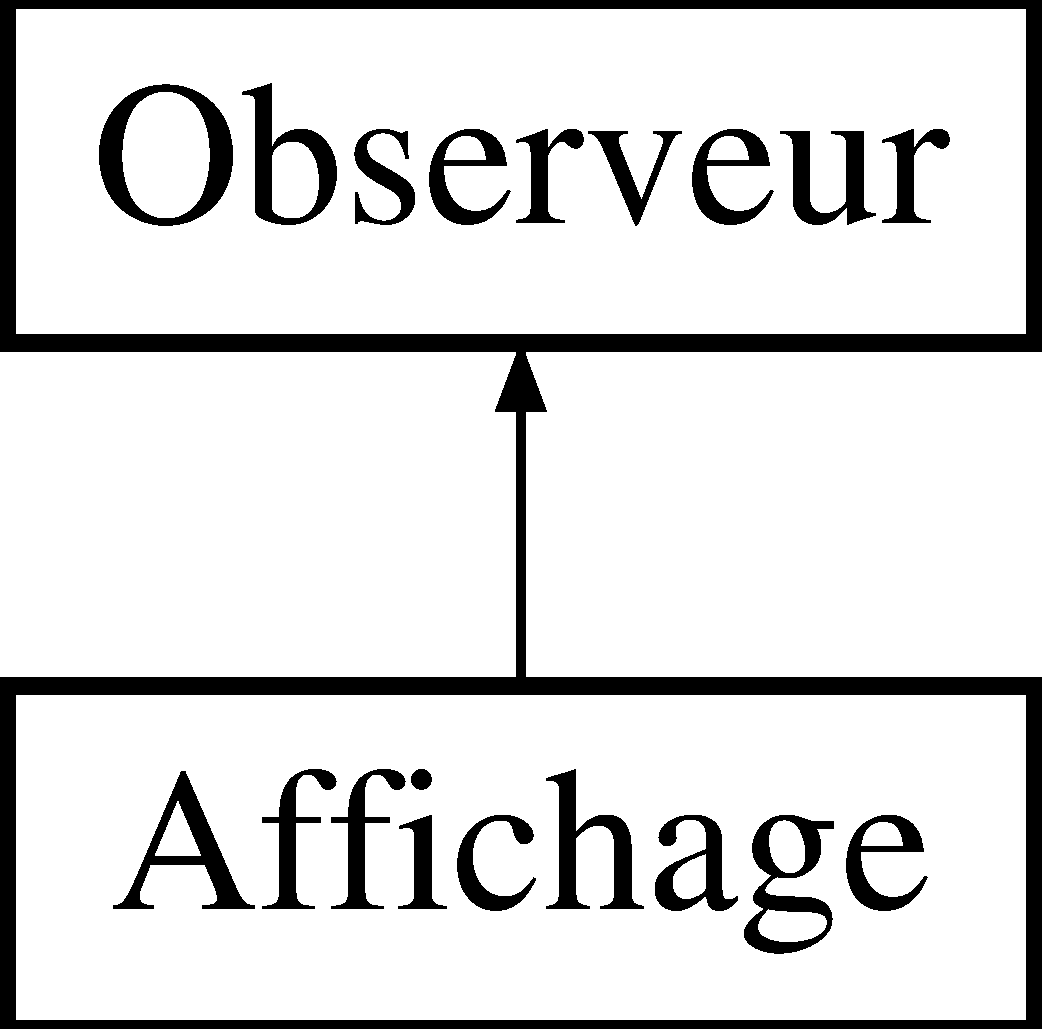
\includegraphics[height=2.000000cm]{class_affichage}
\end{center}
\end{figure}
\subsection*{Fonctions membres publiques}
\begin{DoxyCompactItemize}
\item 
\hyperlink{class_affichage_a7445260b13fa54a65411e810b13ab299}{Affichage} (int res\-X, int res\-Y, std\-::string nom\-\_\-fenetre, \hyperlink{class_jeu}{Jeu} $\ast$j)
\begin{DoxyCompactList}\small\item\em Constructeur. \end{DoxyCompactList}\item 
void \hyperlink{class_affichage_a8ef1dd725b16a7515d0469d9389758ac}{set\-Jeu} (\hyperlink{class_jeu}{Jeu} j)
\begin{DoxyCompactList}\small\item\em Setter. \end{DoxyCompactList}\item 
void \hyperlink{class_affichage_ab8a5da8d3c5a712eceb7c60fc097f076}{update\-Window} ()
\begin{DoxyCompactList}\small\item\em Fait la mise à jour graphique de l'affichage, va regarder dans le jeu observé toutes les valeurs à mettre à jour. \end{DoxyCompactList}\item 
sf\-::\-Render\-Window $\ast$ \hyperlink{class_affichage_a4f102614c071b8dc90a00f136a12d9fd}{get\-Window} ()
\begin{DoxyCompactList}\small\item\em Getter. \end{DoxyCompactList}\item 
void \hyperlink{class_affichage_a76b52d63ae50d54a10bdc27370809a06}{actualiser} ()
\begin{DoxyCompactList}\small\item\em Implémente l'actualisation de la classe observeur. \end{DoxyCompactList}\item 
void \hyperlink{class_affichage_ae9cc540e03d44f364b9266e3ec35e2d1}{fermer} ()
\begin{DoxyCompactList}\small\item\em Ferme la fenetre d'affichage S\-F\-M\-L. \end{DoxyCompactList}\item 
bool \hyperlink{class_affichage_a135fddd2df0e1f2981975cc4ca105265}{est\-Ouvert} ()
\begin{DoxyCompactList}\small\item\em Sert à savoir si la fenetre S\-F\-M\-L est ouverte. \end{DoxyCompactList}\item 
void \hyperlink{class_affichage_afb6dbfbdff30d33ec2cc77393b900e6d}{dessiner\-Infos} ()
\begin{DoxyCompactList}\small\item\em Dessine à l'ecran toutes les infos relatives au jeu, ( à la partie ) \end{DoxyCompactList}\end{DoxyCompactItemize}


\subsection{Description détaillée}
Classe \hyperlink{class_affichage}{Affichage} qui sert à interpreter graphiquement l'état d'un objet \hyperlink{class_jeu}{Jeu}. 

\begin{DoxyDate}{Date}
15/11/2015 
\end{DoxyDate}
\begin{DoxyAuthor}{Auteur}
paul\-\_\-figiel 
\end{DoxyAuthor}


\subsection{Documentation des constructeurs et destructeur}
\hypertarget{class_affichage_a7445260b13fa54a65411e810b13ab299}{\index{Affichage@{Affichage}!Affichage@{Affichage}}
\index{Affichage@{Affichage}!Affichage@{Affichage}}
\subsubsection[{Affichage}]{\setlength{\rightskip}{0pt plus 5cm}Affichage\-::\-Affichage (
\begin{DoxyParamCaption}
\item[{int}]{res\-X, }
\item[{int}]{res\-Y, }
\item[{std\-::string}]{nom\-\_\-fenetre, }
\item[{{\bf Jeu} $\ast$}]{j}
\end{DoxyParamCaption}
)\hspace{0.3cm}{\ttfamily [inline]}}}\label{class_affichage_a7445260b13fa54a65411e810b13ab299}


Constructeur. 

Constructeur de la classe \hyperlink{class_affichage}{Affichage}


\begin{DoxyParams}{Paramètres}
{\em res\-X} & \-: resolution en x de la fenetre \\
\hline
{\em res\-Y} & \-: resolution en y de la fenetre \\
\hline
{\em nom\-\_\-fenetre} & \-: nom de la fenetre \\
\hline
{\em j} & \-: pointeur sur un jeu \\
\hline
\end{DoxyParams}


\subsection{Documentation des fonctions membres}
\hypertarget{class_affichage_a76b52d63ae50d54a10bdc27370809a06}{\index{Affichage@{Affichage}!actualiser@{actualiser}}
\index{actualiser@{actualiser}!Affichage@{Affichage}}
\subsubsection[{actualiser}]{\setlength{\rightskip}{0pt plus 5cm}void Affichage\-::actualiser (
\begin{DoxyParamCaption}
{}
\end{DoxyParamCaption}
)\hspace{0.3cm}{\ttfamily [virtual]}}}\label{class_affichage_a76b52d63ae50d54a10bdc27370809a06}


Implémente l'actualisation de la classe observeur. 



Implémente \hyperlink{class_observeur_ad3f81ed71b0b056e7c20b731211c5958}{Observeur}.

\hypertarget{class_affichage_afb6dbfbdff30d33ec2cc77393b900e6d}{\index{Affichage@{Affichage}!dessiner\-Infos@{dessiner\-Infos}}
\index{dessiner\-Infos@{dessiner\-Infos}!Affichage@{Affichage}}
\subsubsection[{dessiner\-Infos}]{\setlength{\rightskip}{0pt plus 5cm}void Affichage\-::dessiner\-Infos (
\begin{DoxyParamCaption}
{}
\end{DoxyParamCaption}
)}}\label{class_affichage_afb6dbfbdff30d33ec2cc77393b900e6d}


Dessine à l'ecran toutes les infos relatives au jeu, ( à la partie ) 

\hypertarget{class_affichage_a135fddd2df0e1f2981975cc4ca105265}{\index{Affichage@{Affichage}!est\-Ouvert@{est\-Ouvert}}
\index{est\-Ouvert@{est\-Ouvert}!Affichage@{Affichage}}
\subsubsection[{est\-Ouvert}]{\setlength{\rightskip}{0pt plus 5cm}bool Affichage\-::est\-Ouvert (
\begin{DoxyParamCaption}
{}
\end{DoxyParamCaption}
)}}\label{class_affichage_a135fddd2df0e1f2981975cc4ca105265}


Sert à savoir si la fenetre S\-F\-M\-L est ouverte. 

\begin{DoxyReturn}{Renvoie}
true si la fenetre S\-F\-M\-L est ouverte 
\end{DoxyReturn}
\hypertarget{class_affichage_ae9cc540e03d44f364b9266e3ec35e2d1}{\index{Affichage@{Affichage}!fermer@{fermer}}
\index{fermer@{fermer}!Affichage@{Affichage}}
\subsubsection[{fermer}]{\setlength{\rightskip}{0pt plus 5cm}void Affichage\-::fermer (
\begin{DoxyParamCaption}
{}
\end{DoxyParamCaption}
)}}\label{class_affichage_ae9cc540e03d44f364b9266e3ec35e2d1}


Ferme la fenetre d'affichage S\-F\-M\-L. 

\hypertarget{class_affichage_a4f102614c071b8dc90a00f136a12d9fd}{\index{Affichage@{Affichage}!get\-Window@{get\-Window}}
\index{get\-Window@{get\-Window}!Affichage@{Affichage}}
\subsubsection[{get\-Window}]{\setlength{\rightskip}{0pt plus 5cm}sf\-::\-Render\-Window$\ast$ Affichage\-::get\-Window (
\begin{DoxyParamCaption}
{}
\end{DoxyParamCaption}
)\hspace{0.3cm}{\ttfamily [inline]}}}\label{class_affichage_a4f102614c071b8dc90a00f136a12d9fd}


Getter. 

\begin{DoxyReturn}{Renvoie}
window\-\_\- \-: la fenetre d'affichage S\-F\-M\-L utilisée 
\end{DoxyReturn}
\hypertarget{class_affichage_a8ef1dd725b16a7515d0469d9389758ac}{\index{Affichage@{Affichage}!set\-Jeu@{set\-Jeu}}
\index{set\-Jeu@{set\-Jeu}!Affichage@{Affichage}}
\subsubsection[{set\-Jeu}]{\setlength{\rightskip}{0pt plus 5cm}void Affichage\-::set\-Jeu (
\begin{DoxyParamCaption}
\item[{{\bf Jeu}}]{j}
\end{DoxyParamCaption}
)}}\label{class_affichage_a8ef1dd725b16a7515d0469d9389758ac}


Setter. 


\begin{DoxyParams}{Paramètres}
{\em j} & \-: le jeu que l'affichage doit observer \\
\hline
\end{DoxyParams}
\hypertarget{class_affichage_ab8a5da8d3c5a712eceb7c60fc097f076}{\index{Affichage@{Affichage}!update\-Window@{update\-Window}}
\index{update\-Window@{update\-Window}!Affichage@{Affichage}}
\subsubsection[{update\-Window}]{\setlength{\rightskip}{0pt plus 5cm}void Affichage\-::update\-Window (
\begin{DoxyParamCaption}
{}
\end{DoxyParamCaption}
)}}\label{class_affichage_ab8a5da8d3c5a712eceb7c60fc097f076}


Fait la mise à jour graphique de l'affichage, va regarder dans le jeu observé toutes les valeurs à mettre à jour. 



La documentation de cette classe a été générée à partir du fichier suivant \-:\begin{DoxyCompactItemize}
\item 
/home/figiel-\/paul/\-Bureau/\-Projet\-Poo/\-Projet\-P\-O\-O-\/\-A\-R\-A\-Y\-A-\/\-F\-I\-G\-I\-E\-L/include/\hyperlink{_affichage_8hpp}{Affichage.\-hpp}\end{DoxyCompactItemize}

\hypertarget{class_builder_deck}{\section{Référence de la classe Builder\-Deck}
\label{class_builder_deck}\index{Builder\-Deck@{Builder\-Deck}}
}


Classe \hyperlink{class_builder_deck}{Builder\-Deck} qui permet de charger en memoire un deck composé de carte à partir de fichiers txt.  




{\ttfamily \#include $<$Builder\-Deck.\-hpp$>$}

Graphe d'héritage de Builder\-Deck\-:\begin{figure}[H]
\begin{center}
\leavevmode
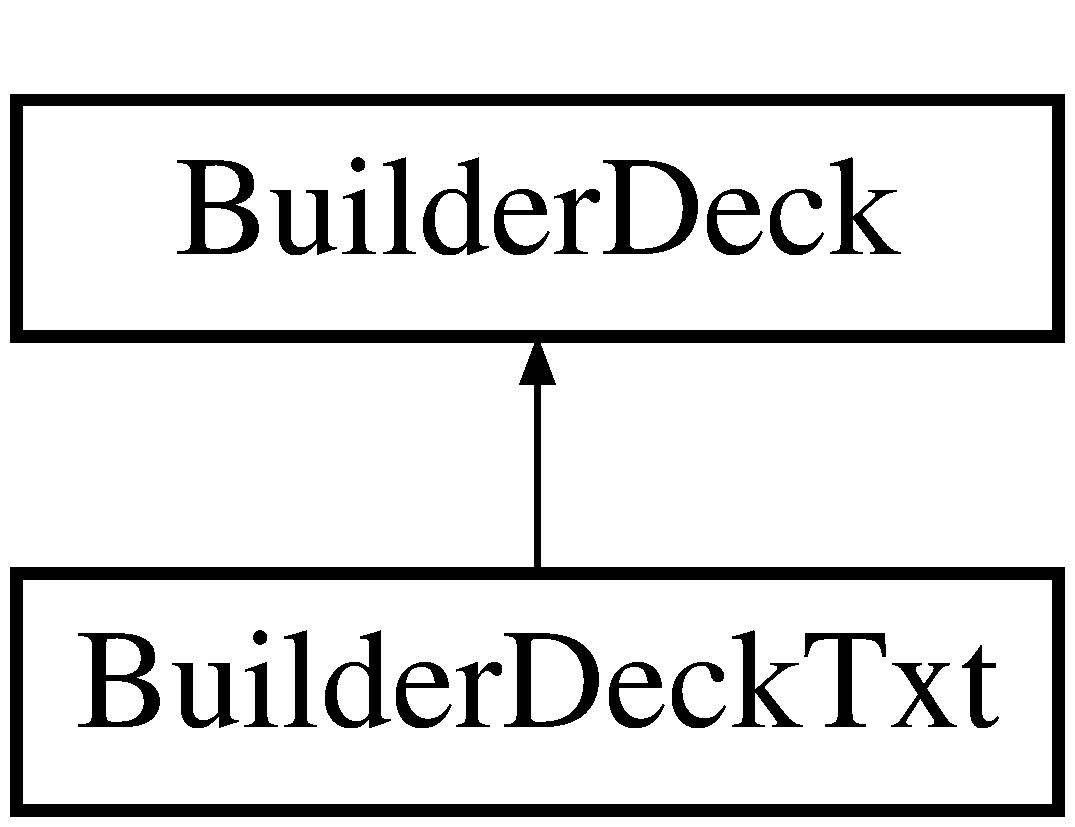
\includegraphics[height=2.000000cm]{class_builder_deck}
\end{center}
\end{figure}
\subsection*{Fonctions membres publiques}
\begin{DoxyCompactItemize}
\item 
virtual \hyperlink{class_carte}{Carte} $\ast$ \hyperlink{class_builder_deck_a6318e704c6b8739fc6666dbc4ab61be2}{creer\-Carte} (std\-::string fichier)=0
\begin{DoxyCompactList}\small\item\em Charge une carte à partir du chemin relatif de son fichier. \end{DoxyCompactList}\item 
virtual \hyperlink{class_champion}{Champion} $\ast$ \hyperlink{class_builder_deck_aeb26090c61c4729af8010b5c4e282389}{creer\-Champion} (std\-::string fichiercarte)=0
\begin{DoxyCompactList}\small\item\em Charge un champion à partir du chemin relatif de son fichier. \end{DoxyCompactList}\item 
virtual void \hyperlink{class_builder_deck_a382f879b47ad1115f4357a3ff0f21e2b}{creer\-Cartes} ()=0
\begin{DoxyCompactList}\small\item\em Rempli le deck de toutes les cartes contenues dans dossier\-\_\-. \end{DoxyCompactList}\item 
virtual \hyperlink{class_deck}{Deck} $\ast$ \hyperlink{class_builder_deck_a8d4db97ac54a8d341591304e3027e7be}{creer\-Deck} ()=0
\begin{DoxyCompactList}\small\item\em Melange les cartes dans deck\-\_\- et le renvoie. \end{DoxyCompactList}\end{DoxyCompactItemize}
\subsection*{Attributs protégés}
\begin{DoxyCompactItemize}
\item 
\hyperlink{class_deck}{Deck} $\ast$ \hyperlink{class_builder_deck_a42b472c027a5a27e2078acabd0f62e76}{deck\-\_\-}
\item 
std\-::string \hyperlink{class_builder_deck_a476542ac85e53c79bbda3cd9ed79dea5}{dossier\-\_\-}
\end{DoxyCompactItemize}


\subsection{Description détaillée}
Classe \hyperlink{class_builder_deck}{Builder\-Deck} qui permet de charger en memoire un deck composé de carte à partir de fichiers txt. 

\begin{DoxyDate}{Date}
15/11/2015 
\end{DoxyDate}
\begin{DoxyAuthor}{Auteur}
paul\-\_\-figiel 
\end{DoxyAuthor}


\subsection{Documentation des fonctions membres}
\hypertarget{class_builder_deck_a6318e704c6b8739fc6666dbc4ab61be2}{\index{Builder\-Deck@{Builder\-Deck}!creer\-Carte@{creer\-Carte}}
\index{creer\-Carte@{creer\-Carte}!BuilderDeck@{Builder\-Deck}}
\subsubsection[{creer\-Carte}]{\setlength{\rightskip}{0pt plus 5cm}virtual {\bf Carte}$\ast$ Builder\-Deck\-::creer\-Carte (
\begin{DoxyParamCaption}
\item[{std\-::string}]{fichier}
\end{DoxyParamCaption}
)\hspace{0.3cm}{\ttfamily [pure virtual]}}}\label{class_builder_deck_a6318e704c6b8739fc6666dbc4ab61be2}


Charge une carte à partir du chemin relatif de son fichier. 


\begin{DoxyParams}{Paramètres}
{\em fichier} & \-: fichier de la carte \\
\hline
\end{DoxyParams}
\begin{DoxyReturn}{Renvoie}
\-: un pointeur sur la carte créé 
\end{DoxyReturn}


Implémenté dans \hyperlink{class_builder_deck_txt_acfb3e111a06efeab6ad47a58edd227bb}{Builder\-Deck\-Txt}.

\hypertarget{class_builder_deck_a382f879b47ad1115f4357a3ff0f21e2b}{\index{Builder\-Deck@{Builder\-Deck}!creer\-Cartes@{creer\-Cartes}}
\index{creer\-Cartes@{creer\-Cartes}!BuilderDeck@{Builder\-Deck}}
\subsubsection[{creer\-Cartes}]{\setlength{\rightskip}{0pt plus 5cm}virtual void Builder\-Deck\-::creer\-Cartes (
\begin{DoxyParamCaption}
{}
\end{DoxyParamCaption}
)\hspace{0.3cm}{\ttfamily [pure virtual]}}}\label{class_builder_deck_a382f879b47ad1115f4357a3ff0f21e2b}


Rempli le deck de toutes les cartes contenues dans dossier\-\_\-. 



Implémenté dans \hyperlink{class_builder_deck_txt_aa4b203ca9600dd92afb07f69d4dd7ec0}{Builder\-Deck\-Txt}.

\hypertarget{class_builder_deck_aeb26090c61c4729af8010b5c4e282389}{\index{Builder\-Deck@{Builder\-Deck}!creer\-Champion@{creer\-Champion}}
\index{creer\-Champion@{creer\-Champion}!BuilderDeck@{Builder\-Deck}}
\subsubsection[{creer\-Champion}]{\setlength{\rightskip}{0pt plus 5cm}virtual {\bf Champion}$\ast$ Builder\-Deck\-::creer\-Champion (
\begin{DoxyParamCaption}
\item[{std\-::string}]{fichiercarte}
\end{DoxyParamCaption}
)\hspace{0.3cm}{\ttfamily [pure virtual]}}}\label{class_builder_deck_aeb26090c61c4729af8010b5c4e282389}


Charge un champion à partir du chemin relatif de son fichier. 


\begin{DoxyParams}{Paramètres}
{\em fichiercarte} & \-: chemin relatif de la carte champion \\
\hline
\end{DoxyParams}
\begin{DoxyReturn}{Renvoie}
\-: pointeur sur le champion créé 
\end{DoxyReturn}


Implémenté dans \hyperlink{class_builder_deck_txt_a232ac1b449e28f535dc6141eac5bb722}{Builder\-Deck\-Txt}.

\hypertarget{class_builder_deck_a8d4db97ac54a8d341591304e3027e7be}{\index{Builder\-Deck@{Builder\-Deck}!creer\-Deck@{creer\-Deck}}
\index{creer\-Deck@{creer\-Deck}!BuilderDeck@{Builder\-Deck}}
\subsubsection[{creer\-Deck}]{\setlength{\rightskip}{0pt plus 5cm}virtual {\bf Deck}$\ast$ Builder\-Deck\-::creer\-Deck (
\begin{DoxyParamCaption}
{}
\end{DoxyParamCaption}
)\hspace{0.3cm}{\ttfamily [pure virtual]}}}\label{class_builder_deck_a8d4db97ac54a8d341591304e3027e7be}


Melange les cartes dans deck\-\_\- et le renvoie. 

\begin{DoxyReturn}{Renvoie}
\-: pointeur sur le deck cree 
\end{DoxyReturn}


Implémenté dans \hyperlink{class_builder_deck_txt_a5f143e781d9d8a879945f96f770eab9a}{Builder\-Deck\-Txt}.



\subsection{Documentation des données membres}
\hypertarget{class_builder_deck_a42b472c027a5a27e2078acabd0f62e76}{\index{Builder\-Deck@{Builder\-Deck}!deck\-\_\-@{deck\-\_\-}}
\index{deck\-\_\-@{deck\-\_\-}!BuilderDeck@{Builder\-Deck}}
\subsubsection[{deck\-\_\-}]{\setlength{\rightskip}{0pt plus 5cm}{\bf Deck}$\ast$ Builder\-Deck\-::deck\-\_\-\hspace{0.3cm}{\ttfamily [protected]}}}\label{class_builder_deck_a42b472c027a5a27e2078acabd0f62e76}
Le deck cree par ce builder \hypertarget{class_builder_deck_a476542ac85e53c79bbda3cd9ed79dea5}{\index{Builder\-Deck@{Builder\-Deck}!dossier\-\_\-@{dossier\-\_\-}}
\index{dossier\-\_\-@{dossier\-\_\-}!BuilderDeck@{Builder\-Deck}}
\subsubsection[{dossier\-\_\-}]{\setlength{\rightskip}{0pt plus 5cm}std\-::string Builder\-Deck\-::dossier\-\_\-\hspace{0.3cm}{\ttfamily [protected]}}}\label{class_builder_deck_a476542ac85e53c79bbda3cd9ed79dea5}
Le dossier ou se trouvent les cartes 

La documentation de cette classe a été générée à partir du fichier suivant \-:\begin{DoxyCompactItemize}
\item 
/home/figiel-\/paul/\-Bureau/\-Projet\-Poo/\-Projet\-P\-O\-O-\/\-A\-R\-A\-Y\-A-\/\-F\-I\-G\-I\-E\-L/include/\hyperlink{_builder_deck_8hpp}{Builder\-Deck.\-hpp}\end{DoxyCompactItemize}

\hypertarget{class_builder_deck_txt}{\section{Référence de la classe Builder\-Deck\-Txt}
\label{class_builder_deck_txt}\index{Builder\-Deck\-Txt@{Builder\-Deck\-Txt}}
}


Classe \hyperlink{class_builder_deck_txt}{Builder\-Deck\-Txt} qui permet de charger en memoire un deck composé de carte à partir de fichiers txt.  




{\ttfamily \#include $<$Builder\-Deck\-Txt.\-hpp$>$}

Graphe d'héritage de Builder\-Deck\-Txt\-:\begin{figure}[H]
\begin{center}
\leavevmode
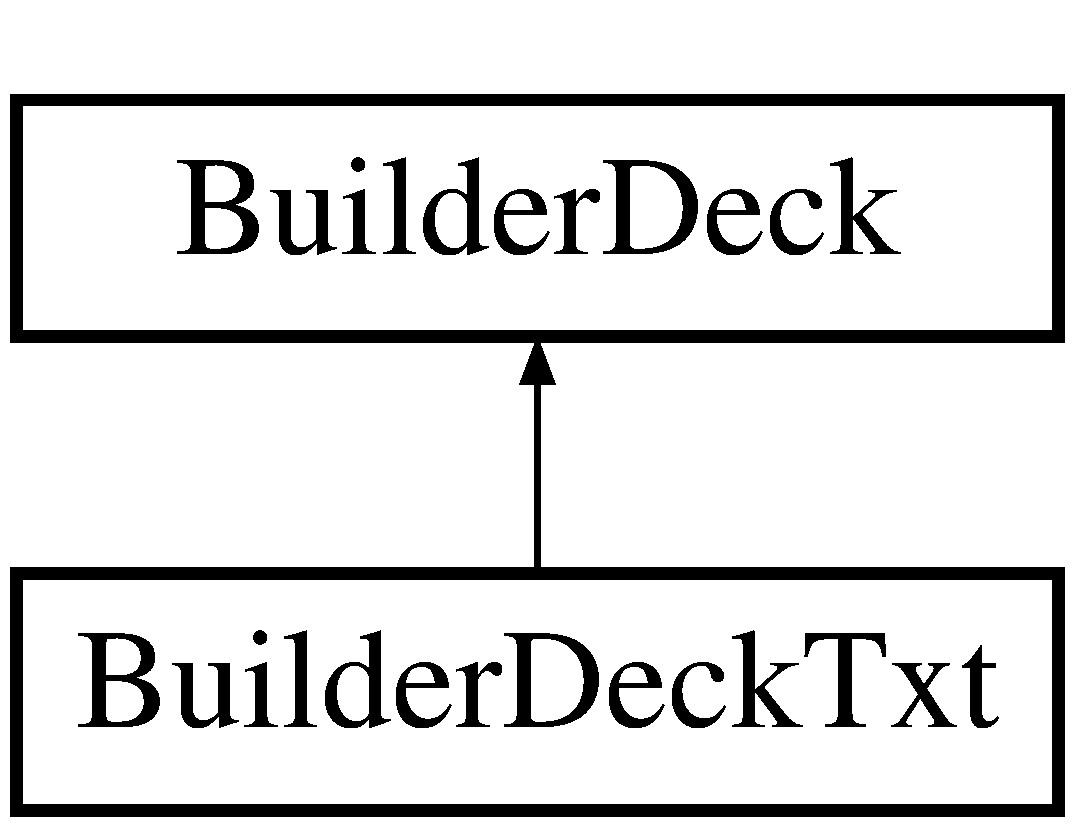
\includegraphics[height=2.000000cm]{class_builder_deck_txt}
\end{center}
\end{figure}
\subsection*{Fonctions membres publiques}
\begin{DoxyCompactItemize}
\item 
\hyperlink{class_builder_deck_txt_add0c11a25020168a94567526a2b3cbfc}{Builder\-Deck\-Txt} (std\-::string dossier)
\begin{DoxyCompactList}\small\item\em Constructeur. \end{DoxyCompactList}\item 
\hyperlink{class_carte}{Carte} $\ast$ \hyperlink{class_builder_deck_txt_acfb3e111a06efeab6ad47a58edd227bb}{creer\-Carte} (std\-::string fichier)
\begin{DoxyCompactList}\small\item\em Charge une carte à partir du chemin relatif de son fichier. \end{DoxyCompactList}\item 
\hyperlink{class_champion}{Champion} $\ast$ \hyperlink{class_builder_deck_txt_a232ac1b449e28f535dc6141eac5bb722}{creer\-Champion} (std\-::string fichiercarte)
\begin{DoxyCompactList}\small\item\em Charge un champion à partir du chemin relatif de son fichier. \end{DoxyCompactList}\item 
void \hyperlink{class_builder_deck_txt_aa4b203ca9600dd92afb07f69d4dd7ec0}{creer\-Cartes} ()
\begin{DoxyCompactList}\small\item\em Rempli le deck de toutes les cartes contenues dans dossier\-\_\-. \end{DoxyCompactList}\item 
\hyperlink{class_deck}{Deck} $\ast$ \hyperlink{class_builder_deck_txt_a5f143e781d9d8a879945f96f770eab9a}{creer\-Deck} ()
\begin{DoxyCompactList}\small\item\em Melange les cartes dans deck\-\_\- et le renvoie. \end{DoxyCompactList}\end{DoxyCompactItemize}
\subsection*{Membres hérités additionnels}


\subsection{Description détaillée}
Classe \hyperlink{class_builder_deck_txt}{Builder\-Deck\-Txt} qui permet de charger en memoire un deck composé de carte à partir de fichiers txt. 

\begin{DoxyDate}{Date}
15/11/2015 
\end{DoxyDate}
\begin{DoxyAuthor}{Auteur}
paul\-\_\-figiel 
\end{DoxyAuthor}


\subsection{Documentation des constructeurs et destructeur}
\hypertarget{class_builder_deck_txt_add0c11a25020168a94567526a2b3cbfc}{\index{Builder\-Deck\-Txt@{Builder\-Deck\-Txt}!Builder\-Deck\-Txt@{Builder\-Deck\-Txt}}
\index{Builder\-Deck\-Txt@{Builder\-Deck\-Txt}!BuilderDeckTxt@{Builder\-Deck\-Txt}}
\subsubsection[{Builder\-Deck\-Txt}]{\setlength{\rightskip}{0pt plus 5cm}Builder\-Deck\-Txt\-::\-Builder\-Deck\-Txt (
\begin{DoxyParamCaption}
\item[{std\-::string}]{dossier}
\end{DoxyParamCaption}
)}}\label{class_builder_deck_txt_add0c11a25020168a94567526a2b3cbfc}


Constructeur. 

Constructeur de la classe \hyperlink{class_builder_deck_txt}{Builder\-Deck\-Txt}


\begin{DoxyParams}{Paramètres}
{\em dossier} & \-: chemin relatif du dossier ou se trouvent les cartes en format txt \\
\hline
\end{DoxyParams}


\subsection{Documentation des fonctions membres}
\hypertarget{class_builder_deck_txt_acfb3e111a06efeab6ad47a58edd227bb}{\index{Builder\-Deck\-Txt@{Builder\-Deck\-Txt}!creer\-Carte@{creer\-Carte}}
\index{creer\-Carte@{creer\-Carte}!BuilderDeckTxt@{Builder\-Deck\-Txt}}
\subsubsection[{creer\-Carte}]{\setlength{\rightskip}{0pt plus 5cm}{\bf Carte}$\ast$ Builder\-Deck\-Txt\-::creer\-Carte (
\begin{DoxyParamCaption}
\item[{std\-::string}]{fichier}
\end{DoxyParamCaption}
)\hspace{0.3cm}{\ttfamily [virtual]}}}\label{class_builder_deck_txt_acfb3e111a06efeab6ad47a58edd227bb}


Charge une carte à partir du chemin relatif de son fichier. 


\begin{DoxyParams}{Paramètres}
{\em fichier} & \-: fichier de la carte \\
\hline
\end{DoxyParams}
\begin{DoxyReturn}{Renvoie}
\-: un pointeur sur la carte créé 
\end{DoxyReturn}


Implémente \hyperlink{class_builder_deck_a6318e704c6b8739fc6666dbc4ab61be2}{Builder\-Deck}.

\hypertarget{class_builder_deck_txt_aa4b203ca9600dd92afb07f69d4dd7ec0}{\index{Builder\-Deck\-Txt@{Builder\-Deck\-Txt}!creer\-Cartes@{creer\-Cartes}}
\index{creer\-Cartes@{creer\-Cartes}!BuilderDeckTxt@{Builder\-Deck\-Txt}}
\subsubsection[{creer\-Cartes}]{\setlength{\rightskip}{0pt plus 5cm}void Builder\-Deck\-Txt\-::creer\-Cartes (
\begin{DoxyParamCaption}
{}
\end{DoxyParamCaption}
)\hspace{0.3cm}{\ttfamily [virtual]}}}\label{class_builder_deck_txt_aa4b203ca9600dd92afb07f69d4dd7ec0}


Rempli le deck de toutes les cartes contenues dans dossier\-\_\-. 



Implémente \hyperlink{class_builder_deck_a382f879b47ad1115f4357a3ff0f21e2b}{Builder\-Deck}.

\hypertarget{class_builder_deck_txt_a232ac1b449e28f535dc6141eac5bb722}{\index{Builder\-Deck\-Txt@{Builder\-Deck\-Txt}!creer\-Champion@{creer\-Champion}}
\index{creer\-Champion@{creer\-Champion}!BuilderDeckTxt@{Builder\-Deck\-Txt}}
\subsubsection[{creer\-Champion}]{\setlength{\rightskip}{0pt plus 5cm}{\bf Champion}$\ast$ Builder\-Deck\-Txt\-::creer\-Champion (
\begin{DoxyParamCaption}
\item[{std\-::string}]{fichiercarte}
\end{DoxyParamCaption}
)\hspace{0.3cm}{\ttfamily [virtual]}}}\label{class_builder_deck_txt_a232ac1b449e28f535dc6141eac5bb722}


Charge un champion à partir du chemin relatif de son fichier. 


\begin{DoxyParams}{Paramètres}
{\em fichiercarte} & \-: chemin relatif de la carte champion \\
\hline
\end{DoxyParams}
\begin{DoxyReturn}{Renvoie}
\-: pointeur sur le champion créé 
\end{DoxyReturn}


Implémente \hyperlink{class_builder_deck_aeb26090c61c4729af8010b5c4e282389}{Builder\-Deck}.

\hypertarget{class_builder_deck_txt_a5f143e781d9d8a879945f96f770eab9a}{\index{Builder\-Deck\-Txt@{Builder\-Deck\-Txt}!creer\-Deck@{creer\-Deck}}
\index{creer\-Deck@{creer\-Deck}!BuilderDeckTxt@{Builder\-Deck\-Txt}}
\subsubsection[{creer\-Deck}]{\setlength{\rightskip}{0pt plus 5cm}{\bf Deck}$\ast$ Builder\-Deck\-Txt\-::creer\-Deck (
\begin{DoxyParamCaption}
{}
\end{DoxyParamCaption}
)\hspace{0.3cm}{\ttfamily [virtual]}}}\label{class_builder_deck_txt_a5f143e781d9d8a879945f96f770eab9a}


Melange les cartes dans deck\-\_\- et le renvoie. 

\begin{DoxyReturn}{Renvoie}
\-: pointeur sur le deck cree 
\end{DoxyReturn}


Implémente \hyperlink{class_builder_deck_a8d4db97ac54a8d341591304e3027e7be}{Builder\-Deck}.



La documentation de cette classe a été générée à partir du fichier suivant \-:\begin{DoxyCompactItemize}
\item 
/home/figiel-\/paul/\-Bureau/\-Projet\-Poo/\-Projet\-P\-O\-O-\/\-A\-R\-A\-Y\-A-\/\-F\-I\-G\-I\-E\-L/include/\hyperlink{_builder_deck_txt_8hpp}{Builder\-Deck\-Txt.\-hpp}\end{DoxyCompactItemize}

\hypertarget{class_carte}{\section{Référence de la classe Carte}
\label{class_carte}\index{Carte@{Carte}}
}


{\ttfamily \#include $<$Carte.\-hpp$>$}

\subsection*{Fonctions membres publiques}
\begin{DoxyCompactItemize}
\item 
\hyperlink{class_carte_a06daaca86c31c80f8308f4a81d46dc9b}{Carte} ()
\begin{DoxyCompactList}\small\item\em Constructeur vide. \end{DoxyCompactList}\item 
\hyperlink{class_carte_a5a1e7bd0334c6cf52ba8991c3a019815}{Carte} (int id, std\-::string nom, int type, std\-::vector$<$ \hyperlink{class_effet}{Effet} $\ast$ $>$ Leffet, int num, int couleur, double F\-S, double dmg)
\begin{DoxyCompactList}\small\item\em Constructeur de carte à 1 coté. \end{DoxyCompactList}\item 
\hyperlink{class_carte_a9fbd39e6a9da16692854ce076ee1a007}{Carte} (int id, std\-::string nom, int type, int type2, std\-::vector$<$ \hyperlink{class_effet}{Effet} $\ast$ $>$ Leffet, std\-::vector$<$ \hyperlink{class_effet}{Effet} $\ast$ $>$ Leffet2, int num, int couleur, double F\-S, double F\-S2, double dmg, double dmg2)
\begin{DoxyCompactList}\small\item\em Constructeur de carte à 1 coté. \end{DoxyCompactList}\item 
\hyperlink{class_carte_a63300ff55c58b5d5b1674a3fc8f25910}{$\sim$\-Carte} ()
\item 
int \hyperlink{class_carte_ae51a40df8fb2ab5498ae67e165ceb5f2}{get\-Id} ()
\item 
void \hyperlink{class_carte_a1aad4c6854631a3de71210d33c15e258}{set\-I\-D} (int id)
\item 
std\-::string \hyperlink{class_carte_a7b68885ddbd8c8f6991e5447346913bc}{get\-Nom} ()
\item 
void \hyperlink{class_carte_a90596fd46a269874d7473afe9733869a}{set\-Nom} (std\-::string nom)
\item 
int \hyperlink{class_carte_aa58ee91b50b7e5e1d2483acb698b59f4}{get\-Type} ()
\item 
int \hyperlink{class_carte_a78fd9aadbd17a4649669117ada726dfa}{get\-Type2} ()
\item 
void \hyperlink{class_carte_a16726786b2df18980f82b9f19d72cd00}{set\-Type} (int type)
\item 
void \hyperlink{class_carte_a78d440deb46f085e53d29cbb81c39c0f}{set\-Type2} (int type)
\item 
std\-::vector$<$ \hyperlink{class_effet}{Effet} $\ast$ $>$ \hyperlink{class_carte_a4410810499a30afcdfe51a70db079dfa}{get\-Leffet} ()
\item 
std\-::vector$<$ \hyperlink{class_effet}{Effet} $\ast$ $>$ \hyperlink{class_carte_ae66d95ae0ba845fe4b5601c36b68cabd}{get\-Leffet2} ()
\item 
void \hyperlink{class_carte_a92a0d5cda40ca72720524937f88f497b}{set\-Leffet} (std\-::vector$<$ \hyperlink{class_effet}{Effet} $\ast$ $>$ Leffet)
\item 
void \hyperlink{class_carte_a1fc20e7a2df33a2ca24ebea22c18f074}{set\-Leffet2} (std\-::vector$<$ \hyperlink{class_effet}{Effet} $\ast$ $>$ Leffet)
\item 
int \hyperlink{class_carte_ae4ede142122a382b2b6648906c4cd37a}{get\-Num} ()
\item 
void \hyperlink{class_carte_a6d5eb0a01948dc48a9c86b7c5083be29}{set\-Num} (int num)
\item 
int \hyperlink{class_carte_a87f5a4affacf484c8e1f308abf4ec514}{get\-Couleur} ()
\item 
void \hyperlink{class_carte_a8736424ac59160d97300befe55b12eea}{set\-Couleur} (int coul)
\item 
bool \hyperlink{class_carte_a4564309a6927eb31e2e0641d1fc80315}{get\-Retournable} ()
\item 
void \hyperlink{class_carte_a53c600ae84b2c9033cede1e147e7de60}{set\-Retournable} (bool r)
\item 
double \hyperlink{class_carte_aac84bc0e598a0c5180ff74e945963a3a}{get\-Fstartup} ()
\item 
double \hyperlink{class_carte_a759d6b7a8b08cf7a6d1e0e5f4e10c28c}{get\-Fstartup2} ()
\item 
double \hyperlink{class_carte_ac742ba23680cb680376984a3b89dcce1}{get\-Face} ()
\item 
void \hyperlink{class_carte_a72278c63fcebe0f1fb38e6f6a49244e9}{set\-Face} (int x)
\item 
void \hyperlink{class_carte_ab3e508c3af45a3e5b38a397b003cc250}{set\-Fstartup} (int F\-S)
\item 
void \hyperlink{class_carte_a82c6e252c3225604e23977e3453af623}{set\-Fstartup2} (int F\-S)
\item 
double \hyperlink{class_carte_a6b831afaa8d2f723ecd642b92de536fb}{get\-Dmg} ()
\item 
double \hyperlink{class_carte_ac6e5febd328ba89c73d755b7edfc61ae}{get\-Dmg2} ()
\item 
void \hyperlink{class_carte_a496ea294465e9ba361ec759b2472da7e}{set\-Dmg} (double dmg)
\item 
void \hyperlink{class_carte_aedb1a92861dec58f566818795efc1e04}{set\-Dmg2} (double dmg2)
\item 
int \hyperlink{class_carte_ad1f2b50c5c627c11547282e88a912d44}{get\-Good\-Type} ()
\begin{DoxyCompactList}\small\item\em Retourne le type de la carte selon son coté ( type\-\_\- si recto type2\-\_\- pour verso) \end{DoxyCompactList}\item 
int \hyperlink{class_carte_a03c8b823ad97a064f6415eea63dcdd3d}{get\-Good\-Fstartup} ()
\begin{DoxyCompactList}\small\item\em Retourne le type de les frame de startup de la carte selon son coté ( Fstartup\-\_\- si recto Fstartup2\-\_\- pour verso) \end{DoxyCompactList}\item 
std\-::vector$<$ \hyperlink{class_effet}{Effet} $\ast$ $>$ \hyperlink{class_carte_aca394e9c23d6b9a8ab7d35e9362295f0}{get\-Good\-Leffet} ()
\begin{DoxyCompactList}\small\item\em Retourne la bonne liste d'effet de la carte selon son coté ( Leffet\-\_\- si recto Leffet2\-\_\- pour verso) \end{DoxyCompactList}\item 
double \hyperlink{class_carte_a3f437815a1d95bb70a9ede79c9f53348}{get\-Good\-Dmg} ()
\begin{DoxyCompactList}\small\item\em Retourne les dommages de la carte selon son coté ( dmg\-\_\- si recto dmg2\-\_\- pour verso) \end{DoxyCompactList}\item 
void \hyperlink{class_carte_ac59034763b08ced32db5d82d080f3ddc}{add\-Effet} (\hyperlink{class_effet}{Effet} $\ast$new\-Effet)
\begin{DoxyCompactList}\small\item\em rajoute un effet à Leffet\-\_\- de la carte \end{DoxyCompactList}\item 
void \hyperlink{class_carte_a3f2cf87d69031210310f6b9eff20fe81}{add\-Effet2} (\hyperlink{class_effet}{Effet} $\ast$new\-Effet)
\begin{DoxyCompactList}\small\item\em rajoute un effet à Leffet2\-\_\- de la carte \end{DoxyCompactList}\item 
void \hyperlink{class_carte_a22cc2da2c3819aeadd1e09e88dfbedcf}{action\-Effet} (\hyperlink{class_jeu}{Jeu} $\ast$jeu, int j)
\begin{DoxyCompactList}\small\item\em apelle action\-Effet de \hyperlink{class_effet}{Effet} sur chaque effet de la carte en prennant en compte le coté ou est tourner la carte \end{DoxyCompactList}\item 
void \hyperlink{class_carte_a007f478e6e0efb44fb4421a94bdacf65}{afficher} ()
\begin{DoxyCompactList}\small\item\em affiche les stats de la carte \end{DoxyCompactList}\item 
bool \hyperlink{class_carte_a54e8a949b343e2c77f3ad8bbbdf0b89a}{changer\-Face} ()
\item 
std\-::string \hyperlink{class_carte_a7f41044fea15a5a73c85e9fbee83114c}{convertion\-Type} (int x)
\begin{DoxyCompactList}\small\item\em convertie les entier 0, 1, ect... indiquant le type de la carte en string \-: coup,choppe ect... pour l'affichage' \end{DoxyCompactList}\item 
std\-::string \hyperlink{class_carte_a9d6b3e60bcd0d08ce097e87ee7e70d3b}{convertion\-Num} ()
\begin{DoxyCompactList}\small\item\em convertie les entier 0, 1, ect... indiquant le numéro de la carte en string \-: 2,3... valet,dame,roi, as \end{DoxyCompactList}\item 
std\-::string \hyperlink{class_carte_a0d9210299570093ca0842df066da50f4}{convertion\-Face} ()
\begin{DoxyCompactList}\small\item\em convertie les entier 0, 1 indiquant le coté de la carte en string \-: recto, verso \end{DoxyCompactList}\item 
std\-::string \hyperlink{class_carte_a9898b43ffbbb68f886dc57f9d72c5f8c}{convertion\-Couleur} ()
\begin{DoxyCompactList}\small\item\em convertie les entier 0, 1, ect... indiquant la couleur de la carte en string \-: coeur,pique... \end{DoxyCompactList}\item 
bool \hyperlink{class_carte_a86d9ef30147380af813336d7fd529521}{equals} (\hyperlink{class_carte}{Carte} $\ast$c)
\begin{DoxyCompactList}\small\item\em regarde si 2 carte sont les même selon leur id \end{DoxyCompactList}\end{DoxyCompactItemize}


\subsection{Documentation des constructeurs et destructeur}
\hypertarget{class_carte_a06daaca86c31c80f8308f4a81d46dc9b}{\index{Carte@{Carte}!Carte@{Carte}}
\index{Carte@{Carte}!Carte@{Carte}}
\subsubsection[{Carte}]{\setlength{\rightskip}{0pt plus 5cm}Carte\-::\-Carte (
\begin{DoxyParamCaption}
{}
\end{DoxyParamCaption}
)\hspace{0.3cm}{\ttfamily [inline]}}}\label{class_carte_a06daaca86c31c80f8308f4a81d46dc9b}


Constructeur vide. 

Constructeur de la classe \hyperlink{class_carte}{Carte} \hypertarget{class_carte_a5a1e7bd0334c6cf52ba8991c3a019815}{\index{Carte@{Carte}!Carte@{Carte}}
\index{Carte@{Carte}!Carte@{Carte}}
\subsubsection[{Carte}]{\setlength{\rightskip}{0pt plus 5cm}Carte\-::\-Carte (
\begin{DoxyParamCaption}
\item[{int}]{id, }
\item[{std\-::string}]{nom, }
\item[{int}]{type, }
\item[{std\-::vector$<$ {\bf Effet} $\ast$ $>$}]{Leffet, }
\item[{int}]{num, }
\item[{int}]{couleur, }
\item[{double}]{F\-S, }
\item[{double}]{dmg}
\end{DoxyParamCaption}
)\hspace{0.3cm}{\ttfamily [inline]}}}\label{class_carte_a5a1e7bd0334c6cf52ba8991c3a019815}


Constructeur de carte à 1 coté. 

Constructeur de la classe \hyperlink{class_carte}{Carte}


\begin{DoxyParams}{Paramètres}
{\em id} & \-: id de la carte \\
\hline
{\em nom} & \-: nom de la carte \\
\hline
{\em Leffet} & \-: liste des effets de la carte \\
\hline
{\em } & type \-: type de la carte \\
\hline
{\em num} & \-: numéro de la carte \\
\hline
{\em couleur} & \-: couleur de la carte \\
\hline
{\em F\-S} & \-: framed de startup de la carte \\
\hline
{\em dmg} & \-: dommage de la carte \\
\hline
\end{DoxyParams}
\hypertarget{class_carte_a9fbd39e6a9da16692854ce076ee1a007}{\index{Carte@{Carte}!Carte@{Carte}}
\index{Carte@{Carte}!Carte@{Carte}}
\subsubsection[{Carte}]{\setlength{\rightskip}{0pt plus 5cm}Carte\-::\-Carte (
\begin{DoxyParamCaption}
\item[{int}]{id, }
\item[{std\-::string}]{nom, }
\item[{int}]{type, }
\item[{int}]{type2, }
\item[{std\-::vector$<$ {\bf Effet} $\ast$ $>$}]{Leffet, }
\item[{std\-::vector$<$ {\bf Effet} $\ast$ $>$}]{Leffet2, }
\item[{int}]{num, }
\item[{int}]{couleur, }
\item[{double}]{F\-S, }
\item[{double}]{F\-S2, }
\item[{double}]{dmg, }
\item[{double}]{dmg2}
\end{DoxyParamCaption}
)\hspace{0.3cm}{\ttfamily [inline]}}}\label{class_carte_a9fbd39e6a9da16692854ce076ee1a007}


Constructeur de carte à 1 coté. 

Constructeur de la classe \hyperlink{class_carte}{Carte}


\begin{DoxyParams}{Paramètres}
{\em id} & \-: id de la carte \\
\hline
{\em nom} & \-: nom de la carte \\
\hline
{\em Leffet} & \-: liste des effets de la carte coté recto \\
\hline
{\em Leffet2} & \-: liste des effets de la carte coté verso \\
\hline
{\em } & type \-: type de la carte coté recto \\
\hline
{\em } & type2 \-: type de la carte coté verso \\
\hline
{\em num} & \-: numéro de la carte \\
\hline
{\em couleur} & \-: couleur de la carte \\
\hline
{\em F\-S} & \-: framed de startup de la carte coté recto \\
\hline
{\em F\-S2} & \-: framed de startup de la carte coté verso \\
\hline
{\em dmg} & \-: dommage de la carte coté recto \\
\hline
{\em dmg2} & \-: dommage de la carte coté verso \\
\hline
\end{DoxyParams}
\hypertarget{class_carte_a63300ff55c58b5d5b1674a3fc8f25910}{\index{Carte@{Carte}!$\sim$\-Carte@{$\sim$\-Carte}}
\index{$\sim$\-Carte@{$\sim$\-Carte}!Carte@{Carte}}
\subsubsection[{$\sim$\-Carte}]{\setlength{\rightskip}{0pt plus 5cm}Carte\-::$\sim$\-Carte (
\begin{DoxyParamCaption}
{}
\end{DoxyParamCaption}
)}}\label{class_carte_a63300ff55c58b5d5b1674a3fc8f25910}


\subsection{Documentation des fonctions membres}
\hypertarget{class_carte_a22cc2da2c3819aeadd1e09e88dfbedcf}{\index{Carte@{Carte}!action\-Effet@{action\-Effet}}
\index{action\-Effet@{action\-Effet}!Carte@{Carte}}
\subsubsection[{action\-Effet}]{\setlength{\rightskip}{0pt plus 5cm}void Carte\-::action\-Effet (
\begin{DoxyParamCaption}
\item[{{\bf Jeu} $\ast$}]{jeu, }
\item[{int}]{j}
\end{DoxyParamCaption}
)}}\label{class_carte_a22cc2da2c3819aeadd1e09e88dfbedcf}


apelle action\-Effet de \hyperlink{class_effet}{Effet} sur chaque effet de la carte en prennant en compte le coté ou est tourner la carte 


\begin{DoxyParams}{Paramètres}
{\em \hyperlink{class_jeu}{Jeu}} & $\ast$jeu \-: Le jeu \\
\hline
{\em int} & j \-: un entier indiquant qu'elle joueur joue la carte \\
\hline
\end{DoxyParams}
\hypertarget{class_carte_ac59034763b08ced32db5d82d080f3ddc}{\index{Carte@{Carte}!add\-Effet@{add\-Effet}}
\index{add\-Effet@{add\-Effet}!Carte@{Carte}}
\subsubsection[{add\-Effet}]{\setlength{\rightskip}{0pt plus 5cm}void Carte\-::add\-Effet (
\begin{DoxyParamCaption}
\item[{{\bf Effet} $\ast$}]{new\-Effet}
\end{DoxyParamCaption}
)}}\label{class_carte_ac59034763b08ced32db5d82d080f3ddc}


rajoute un effet à Leffet\-\_\- de la carte 


\begin{DoxyParams}{Paramètres}
{\em new\-Effet} & \-: l'effet à rajouté \\
\hline
\end{DoxyParams}
\hypertarget{class_carte_a3f2cf87d69031210310f6b9eff20fe81}{\index{Carte@{Carte}!add\-Effet2@{add\-Effet2}}
\index{add\-Effet2@{add\-Effet2}!Carte@{Carte}}
\subsubsection[{add\-Effet2}]{\setlength{\rightskip}{0pt plus 5cm}void Carte\-::add\-Effet2 (
\begin{DoxyParamCaption}
\item[{{\bf Effet} $\ast$}]{new\-Effet}
\end{DoxyParamCaption}
)}}\label{class_carte_a3f2cf87d69031210310f6b9eff20fe81}


rajoute un effet à Leffet2\-\_\- de la carte 


\begin{DoxyParams}{Paramètres}
{\em new\-Effet} & \-: l'effet à rajouté \\
\hline
\end{DoxyParams}
\hypertarget{class_carte_a007f478e6e0efb44fb4421a94bdacf65}{\index{Carte@{Carte}!afficher@{afficher}}
\index{afficher@{afficher}!Carte@{Carte}}
\subsubsection[{afficher}]{\setlength{\rightskip}{0pt plus 5cm}void Carte\-::afficher (
\begin{DoxyParamCaption}
{}
\end{DoxyParamCaption}
)}}\label{class_carte_a007f478e6e0efb44fb4421a94bdacf65}


affiche les stats de la carte 

\hypertarget{class_carte_a54e8a949b343e2c77f3ad8bbbdf0b89a}{\index{Carte@{Carte}!changer\-Face@{changer\-Face}}
\index{changer\-Face@{changer\-Face}!Carte@{Carte}}
\subsubsection[{changer\-Face}]{\setlength{\rightskip}{0pt plus 5cm}bool Carte\-::changer\-Face (
\begin{DoxyParamCaption}
{}
\end{DoxyParamCaption}
)}}\label{class_carte_a54e8a949b343e2c77f3ad8bbbdf0b89a}
la carte sur son autre coté si possible \hypertarget{class_carte_a9898b43ffbbb68f886dc57f9d72c5f8c}{\index{Carte@{Carte}!convertion\-Couleur@{convertion\-Couleur}}
\index{convertion\-Couleur@{convertion\-Couleur}!Carte@{Carte}}
\subsubsection[{convertion\-Couleur}]{\setlength{\rightskip}{0pt plus 5cm}std\-::string Carte\-::convertion\-Couleur (
\begin{DoxyParamCaption}
{}
\end{DoxyParamCaption}
)}}\label{class_carte_a9898b43ffbbb68f886dc57f9d72c5f8c}


convertie les entier 0, 1, ect... indiquant la couleur de la carte en string \-: coeur,pique... 

un string indiquant la couleurla carte \hypertarget{class_carte_a0d9210299570093ca0842df066da50f4}{\index{Carte@{Carte}!convertion\-Face@{convertion\-Face}}
\index{convertion\-Face@{convertion\-Face}!Carte@{Carte}}
\subsubsection[{convertion\-Face}]{\setlength{\rightskip}{0pt plus 5cm}std\-::string Carte\-::convertion\-Face (
\begin{DoxyParamCaption}
{}
\end{DoxyParamCaption}
)}}\label{class_carte_a0d9210299570093ca0842df066da50f4}


convertie les entier 0, 1 indiquant le coté de la carte en string \-: recto, verso 

un string indiquant le coté de la carte ( recto / verso) \hypertarget{class_carte_a9d6b3e60bcd0d08ce097e87ee7e70d3b}{\index{Carte@{Carte}!convertion\-Num@{convertion\-Num}}
\index{convertion\-Num@{convertion\-Num}!Carte@{Carte}}
\subsubsection[{convertion\-Num}]{\setlength{\rightskip}{0pt plus 5cm}std\-::string Carte\-::convertion\-Num (
\begin{DoxyParamCaption}
{}
\end{DoxyParamCaption}
)}}\label{class_carte_a9d6b3e60bcd0d08ce097e87ee7e70d3b}


convertie les entier 0, 1, ect... indiquant le numéro de la carte en string \-: 2,3... valet,dame,roi, as 

un string indiquant le numéro de la carte \hypertarget{class_carte_a7f41044fea15a5a73c85e9fbee83114c}{\index{Carte@{Carte}!convertion\-Type@{convertion\-Type}}
\index{convertion\-Type@{convertion\-Type}!Carte@{Carte}}
\subsubsection[{convertion\-Type}]{\setlength{\rightskip}{0pt plus 5cm}std\-::string Carte\-::convertion\-Type (
\begin{DoxyParamCaption}
\item[{int}]{x}
\end{DoxyParamCaption}
)}}\label{class_carte_a7f41044fea15a5a73c85e9fbee83114c}


convertie les entier 0, 1, ect... indiquant le type de la carte en string \-: coup,choppe ect... pour l'affichage' 


\begin{DoxyParams}{Paramètres}
{\em entier} & x \-: indique de qe quel coté on veut indiqué le type  un string indiquant le type de la carte \\
\hline
\end{DoxyParams}
\hypertarget{class_carte_a86d9ef30147380af813336d7fd529521}{\index{Carte@{Carte}!equals@{equals}}
\index{equals@{equals}!Carte@{Carte}}
\subsubsection[{equals}]{\setlength{\rightskip}{0pt plus 5cm}bool Carte\-::equals (
\begin{DoxyParamCaption}
\item[{{\bf Carte} $\ast$}]{c}
\end{DoxyParamCaption}
)}}\label{class_carte_a86d9ef30147380af813336d7fd529521}


regarde si 2 carte sont les même selon leur id 


\begin{DoxyParams}{Paramètres}
{\em c} & \-: pointeur vers la seconde carte  true si l'id des deux cartes sont la même sinon retourne fasle \\
\hline
\end{DoxyParams}
\hypertarget{class_carte_a87f5a4affacf484c8e1f308abf4ec514}{\index{Carte@{Carte}!get\-Couleur@{get\-Couleur}}
\index{get\-Couleur@{get\-Couleur}!Carte@{Carte}}
\subsubsection[{get\-Couleur}]{\setlength{\rightskip}{0pt plus 5cm}int Carte\-::get\-Couleur (
\begin{DoxyParamCaption}
{}
\end{DoxyParamCaption}
)\hspace{0.3cm}{\ttfamily [inline]}}}\label{class_carte_a87f5a4affacf484c8e1f308abf4ec514}
\hypertarget{class_carte_a6b831afaa8d2f723ecd642b92de536fb}{\index{Carte@{Carte}!get\-Dmg@{get\-Dmg}}
\index{get\-Dmg@{get\-Dmg}!Carte@{Carte}}
\subsubsection[{get\-Dmg}]{\setlength{\rightskip}{0pt plus 5cm}double Carte\-::get\-Dmg (
\begin{DoxyParamCaption}
{}
\end{DoxyParamCaption}
)\hspace{0.3cm}{\ttfamily [inline]}}}\label{class_carte_a6b831afaa8d2f723ecd642b92de536fb}
\hypertarget{class_carte_ac6e5febd328ba89c73d755b7edfc61ae}{\index{Carte@{Carte}!get\-Dmg2@{get\-Dmg2}}
\index{get\-Dmg2@{get\-Dmg2}!Carte@{Carte}}
\subsubsection[{get\-Dmg2}]{\setlength{\rightskip}{0pt plus 5cm}double Carte\-::get\-Dmg2 (
\begin{DoxyParamCaption}
{}
\end{DoxyParamCaption}
)\hspace{0.3cm}{\ttfamily [inline]}}}\label{class_carte_ac6e5febd328ba89c73d755b7edfc61ae}
\hypertarget{class_carte_ac742ba23680cb680376984a3b89dcce1}{\index{Carte@{Carte}!get\-Face@{get\-Face}}
\index{get\-Face@{get\-Face}!Carte@{Carte}}
\subsubsection[{get\-Face}]{\setlength{\rightskip}{0pt plus 5cm}double Carte\-::get\-Face (
\begin{DoxyParamCaption}
{}
\end{DoxyParamCaption}
)\hspace{0.3cm}{\ttfamily [inline]}}}\label{class_carte_ac742ba23680cb680376984a3b89dcce1}
\hypertarget{class_carte_aac84bc0e598a0c5180ff74e945963a3a}{\index{Carte@{Carte}!get\-Fstartup@{get\-Fstartup}}
\index{get\-Fstartup@{get\-Fstartup}!Carte@{Carte}}
\subsubsection[{get\-Fstartup}]{\setlength{\rightskip}{0pt plus 5cm}double Carte\-::get\-Fstartup (
\begin{DoxyParamCaption}
{}
\end{DoxyParamCaption}
)\hspace{0.3cm}{\ttfamily [inline]}}}\label{class_carte_aac84bc0e598a0c5180ff74e945963a3a}
\hypertarget{class_carte_a759d6b7a8b08cf7a6d1e0e5f4e10c28c}{\index{Carte@{Carte}!get\-Fstartup2@{get\-Fstartup2}}
\index{get\-Fstartup2@{get\-Fstartup2}!Carte@{Carte}}
\subsubsection[{get\-Fstartup2}]{\setlength{\rightskip}{0pt plus 5cm}double Carte\-::get\-Fstartup2 (
\begin{DoxyParamCaption}
{}
\end{DoxyParamCaption}
)\hspace{0.3cm}{\ttfamily [inline]}}}\label{class_carte_a759d6b7a8b08cf7a6d1e0e5f4e10c28c}
\hypertarget{class_carte_a3f437815a1d95bb70a9ede79c9f53348}{\index{Carte@{Carte}!get\-Good\-Dmg@{get\-Good\-Dmg}}
\index{get\-Good\-Dmg@{get\-Good\-Dmg}!Carte@{Carte}}
\subsubsection[{get\-Good\-Dmg}]{\setlength{\rightskip}{0pt plus 5cm}double Carte\-::get\-Good\-Dmg (
\begin{DoxyParamCaption}
{}
\end{DoxyParamCaption}
)}}\label{class_carte_a3f437815a1d95bb70a9ede79c9f53348}


Retourne les dommages de la carte selon son coté ( dmg\-\_\- si recto dmg2\-\_\- pour verso) 

\begin{DoxyReturn}{Renvoie}
\-: un double indiquand les dommages de la carte 
\end{DoxyReturn}
\hypertarget{class_carte_a03c8b823ad97a064f6415eea63dcdd3d}{\index{Carte@{Carte}!get\-Good\-Fstartup@{get\-Good\-Fstartup}}
\index{get\-Good\-Fstartup@{get\-Good\-Fstartup}!Carte@{Carte}}
\subsubsection[{get\-Good\-Fstartup}]{\setlength{\rightskip}{0pt plus 5cm}int Carte\-::get\-Good\-Fstartup (
\begin{DoxyParamCaption}
{}
\end{DoxyParamCaption}
)}}\label{class_carte_a03c8b823ad97a064f6415eea63dcdd3d}


Retourne le type de les frame de startup de la carte selon son coté ( Fstartup\-\_\- si recto Fstartup2\-\_\- pour verso) 

\begin{DoxyReturn}{Renvoie}
\-: un int indiquant les frame de startup de la carte 
\end{DoxyReturn}
\hypertarget{class_carte_aca394e9c23d6b9a8ab7d35e9362295f0}{\index{Carte@{Carte}!get\-Good\-Leffet@{get\-Good\-Leffet}}
\index{get\-Good\-Leffet@{get\-Good\-Leffet}!Carte@{Carte}}
\subsubsection[{get\-Good\-Leffet}]{\setlength{\rightskip}{0pt plus 5cm}std\-::vector$<${\bf Effet}$\ast$$>$ Carte\-::get\-Good\-Leffet (
\begin{DoxyParamCaption}
{}
\end{DoxyParamCaption}
)}}\label{class_carte_aca394e9c23d6b9a8ab7d35e9362295f0}


Retourne la bonne liste d'effet de la carte selon son coté ( Leffet\-\_\- si recto Leffet2\-\_\- pour verso) 

\begin{DoxyReturn}{Renvoie}
\-: un vector$<$\-Effet$\ast$$>$ 
\end{DoxyReturn}
\hypertarget{class_carte_ad1f2b50c5c627c11547282e88a912d44}{\index{Carte@{Carte}!get\-Good\-Type@{get\-Good\-Type}}
\index{get\-Good\-Type@{get\-Good\-Type}!Carte@{Carte}}
\subsubsection[{get\-Good\-Type}]{\setlength{\rightskip}{0pt plus 5cm}int Carte\-::get\-Good\-Type (
\begin{DoxyParamCaption}
{}
\end{DoxyParamCaption}
)}}\label{class_carte_ad1f2b50c5c627c11547282e88a912d44}


Retourne le type de la carte selon son coté ( type\-\_\- si recto type2\-\_\- pour verso) 

\begin{DoxyReturn}{Renvoie}
\-: un int indiquant le type de la carte 
\end{DoxyReturn}
\hypertarget{class_carte_ae51a40df8fb2ab5498ae67e165ceb5f2}{\index{Carte@{Carte}!get\-Id@{get\-Id}}
\index{get\-Id@{get\-Id}!Carte@{Carte}}
\subsubsection[{get\-Id}]{\setlength{\rightskip}{0pt plus 5cm}int Carte\-::get\-Id (
\begin{DoxyParamCaption}
{}
\end{DoxyParamCaption}
)\hspace{0.3cm}{\ttfamily [inline]}}}\label{class_carte_ae51a40df8fb2ab5498ae67e165ceb5f2}
\hypertarget{class_carte_a4410810499a30afcdfe51a70db079dfa}{\index{Carte@{Carte}!get\-Leffet@{get\-Leffet}}
\index{get\-Leffet@{get\-Leffet}!Carte@{Carte}}
\subsubsection[{get\-Leffet}]{\setlength{\rightskip}{0pt plus 5cm}std\-::vector$<${\bf Effet}$\ast$$>$ Carte\-::get\-Leffet (
\begin{DoxyParamCaption}
{}
\end{DoxyParamCaption}
)\hspace{0.3cm}{\ttfamily [inline]}}}\label{class_carte_a4410810499a30afcdfe51a70db079dfa}
\hypertarget{class_carte_ae66d95ae0ba845fe4b5601c36b68cabd}{\index{Carte@{Carte}!get\-Leffet2@{get\-Leffet2}}
\index{get\-Leffet2@{get\-Leffet2}!Carte@{Carte}}
\subsubsection[{get\-Leffet2}]{\setlength{\rightskip}{0pt plus 5cm}std\-::vector$<${\bf Effet}$\ast$$>$ Carte\-::get\-Leffet2 (
\begin{DoxyParamCaption}
{}
\end{DoxyParamCaption}
)\hspace{0.3cm}{\ttfamily [inline]}}}\label{class_carte_ae66d95ae0ba845fe4b5601c36b68cabd}
\hypertarget{class_carte_a7b68885ddbd8c8f6991e5447346913bc}{\index{Carte@{Carte}!get\-Nom@{get\-Nom}}
\index{get\-Nom@{get\-Nom}!Carte@{Carte}}
\subsubsection[{get\-Nom}]{\setlength{\rightskip}{0pt plus 5cm}std\-::string Carte\-::get\-Nom (
\begin{DoxyParamCaption}
{}
\end{DoxyParamCaption}
)\hspace{0.3cm}{\ttfamily [inline]}}}\label{class_carte_a7b68885ddbd8c8f6991e5447346913bc}
\hypertarget{class_carte_ae4ede142122a382b2b6648906c4cd37a}{\index{Carte@{Carte}!get\-Num@{get\-Num}}
\index{get\-Num@{get\-Num}!Carte@{Carte}}
\subsubsection[{get\-Num}]{\setlength{\rightskip}{0pt plus 5cm}int Carte\-::get\-Num (
\begin{DoxyParamCaption}
{}
\end{DoxyParamCaption}
)\hspace{0.3cm}{\ttfamily [inline]}}}\label{class_carte_ae4ede142122a382b2b6648906c4cd37a}
\hypertarget{class_carte_a4564309a6927eb31e2e0641d1fc80315}{\index{Carte@{Carte}!get\-Retournable@{get\-Retournable}}
\index{get\-Retournable@{get\-Retournable}!Carte@{Carte}}
\subsubsection[{get\-Retournable}]{\setlength{\rightskip}{0pt plus 5cm}bool Carte\-::get\-Retournable (
\begin{DoxyParamCaption}
{}
\end{DoxyParamCaption}
)\hspace{0.3cm}{\ttfamily [inline]}}}\label{class_carte_a4564309a6927eb31e2e0641d1fc80315}
\hypertarget{class_carte_aa58ee91b50b7e5e1d2483acb698b59f4}{\index{Carte@{Carte}!get\-Type@{get\-Type}}
\index{get\-Type@{get\-Type}!Carte@{Carte}}
\subsubsection[{get\-Type}]{\setlength{\rightskip}{0pt plus 5cm}int Carte\-::get\-Type (
\begin{DoxyParamCaption}
{}
\end{DoxyParamCaption}
)\hspace{0.3cm}{\ttfamily [inline]}}}\label{class_carte_aa58ee91b50b7e5e1d2483acb698b59f4}
\hypertarget{class_carte_a78fd9aadbd17a4649669117ada726dfa}{\index{Carte@{Carte}!get\-Type2@{get\-Type2}}
\index{get\-Type2@{get\-Type2}!Carte@{Carte}}
\subsubsection[{get\-Type2}]{\setlength{\rightskip}{0pt plus 5cm}int Carte\-::get\-Type2 (
\begin{DoxyParamCaption}
{}
\end{DoxyParamCaption}
)\hspace{0.3cm}{\ttfamily [inline]}}}\label{class_carte_a78fd9aadbd17a4649669117ada726dfa}
\hypertarget{class_carte_a8736424ac59160d97300befe55b12eea}{\index{Carte@{Carte}!set\-Couleur@{set\-Couleur}}
\index{set\-Couleur@{set\-Couleur}!Carte@{Carte}}
\subsubsection[{set\-Couleur}]{\setlength{\rightskip}{0pt plus 5cm}void Carte\-::set\-Couleur (
\begin{DoxyParamCaption}
\item[{int}]{coul}
\end{DoxyParamCaption}
)\hspace{0.3cm}{\ttfamily [inline]}}}\label{class_carte_a8736424ac59160d97300befe55b12eea}
\hypertarget{class_carte_a496ea294465e9ba361ec759b2472da7e}{\index{Carte@{Carte}!set\-Dmg@{set\-Dmg}}
\index{set\-Dmg@{set\-Dmg}!Carte@{Carte}}
\subsubsection[{set\-Dmg}]{\setlength{\rightskip}{0pt plus 5cm}void Carte\-::set\-Dmg (
\begin{DoxyParamCaption}
\item[{double}]{dmg}
\end{DoxyParamCaption}
)\hspace{0.3cm}{\ttfamily [inline]}}}\label{class_carte_a496ea294465e9ba361ec759b2472da7e}
\hypertarget{class_carte_aedb1a92861dec58f566818795efc1e04}{\index{Carte@{Carte}!set\-Dmg2@{set\-Dmg2}}
\index{set\-Dmg2@{set\-Dmg2}!Carte@{Carte}}
\subsubsection[{set\-Dmg2}]{\setlength{\rightskip}{0pt plus 5cm}void Carte\-::set\-Dmg2 (
\begin{DoxyParamCaption}
\item[{double}]{dmg2}
\end{DoxyParamCaption}
)\hspace{0.3cm}{\ttfamily [inline]}}}\label{class_carte_aedb1a92861dec58f566818795efc1e04}
\hypertarget{class_carte_a72278c63fcebe0f1fb38e6f6a49244e9}{\index{Carte@{Carte}!set\-Face@{set\-Face}}
\index{set\-Face@{set\-Face}!Carte@{Carte}}
\subsubsection[{set\-Face}]{\setlength{\rightskip}{0pt plus 5cm}void Carte\-::set\-Face (
\begin{DoxyParamCaption}
\item[{int}]{x}
\end{DoxyParamCaption}
)\hspace{0.3cm}{\ttfamily [inline]}}}\label{class_carte_a72278c63fcebe0f1fb38e6f6a49244e9}
\hypertarget{class_carte_ab3e508c3af45a3e5b38a397b003cc250}{\index{Carte@{Carte}!set\-Fstartup@{set\-Fstartup}}
\index{set\-Fstartup@{set\-Fstartup}!Carte@{Carte}}
\subsubsection[{set\-Fstartup}]{\setlength{\rightskip}{0pt plus 5cm}void Carte\-::set\-Fstartup (
\begin{DoxyParamCaption}
\item[{int}]{F\-S}
\end{DoxyParamCaption}
)\hspace{0.3cm}{\ttfamily [inline]}}}\label{class_carte_ab3e508c3af45a3e5b38a397b003cc250}
\hypertarget{class_carte_a82c6e252c3225604e23977e3453af623}{\index{Carte@{Carte}!set\-Fstartup2@{set\-Fstartup2}}
\index{set\-Fstartup2@{set\-Fstartup2}!Carte@{Carte}}
\subsubsection[{set\-Fstartup2}]{\setlength{\rightskip}{0pt plus 5cm}void Carte\-::set\-Fstartup2 (
\begin{DoxyParamCaption}
\item[{int}]{F\-S}
\end{DoxyParamCaption}
)\hspace{0.3cm}{\ttfamily [inline]}}}\label{class_carte_a82c6e252c3225604e23977e3453af623}
\hypertarget{class_carte_a1aad4c6854631a3de71210d33c15e258}{\index{Carte@{Carte}!set\-I\-D@{set\-I\-D}}
\index{set\-I\-D@{set\-I\-D}!Carte@{Carte}}
\subsubsection[{set\-I\-D}]{\setlength{\rightskip}{0pt plus 5cm}void Carte\-::set\-I\-D (
\begin{DoxyParamCaption}
\item[{int}]{id}
\end{DoxyParamCaption}
)\hspace{0.3cm}{\ttfamily [inline]}}}\label{class_carte_a1aad4c6854631a3de71210d33c15e258}
\hypertarget{class_carte_a92a0d5cda40ca72720524937f88f497b}{\index{Carte@{Carte}!set\-Leffet@{set\-Leffet}}
\index{set\-Leffet@{set\-Leffet}!Carte@{Carte}}
\subsubsection[{set\-Leffet}]{\setlength{\rightskip}{0pt plus 5cm}void Carte\-::set\-Leffet (
\begin{DoxyParamCaption}
\item[{std\-::vector$<$ {\bf Effet} $\ast$ $>$}]{Leffet}
\end{DoxyParamCaption}
)\hspace{0.3cm}{\ttfamily [inline]}}}\label{class_carte_a92a0d5cda40ca72720524937f88f497b}
\hypertarget{class_carte_a1fc20e7a2df33a2ca24ebea22c18f074}{\index{Carte@{Carte}!set\-Leffet2@{set\-Leffet2}}
\index{set\-Leffet2@{set\-Leffet2}!Carte@{Carte}}
\subsubsection[{set\-Leffet2}]{\setlength{\rightskip}{0pt plus 5cm}void Carte\-::set\-Leffet2 (
\begin{DoxyParamCaption}
\item[{std\-::vector$<$ {\bf Effet} $\ast$ $>$}]{Leffet}
\end{DoxyParamCaption}
)\hspace{0.3cm}{\ttfamily [inline]}}}\label{class_carte_a1fc20e7a2df33a2ca24ebea22c18f074}
\hypertarget{class_carte_a90596fd46a269874d7473afe9733869a}{\index{Carte@{Carte}!set\-Nom@{set\-Nom}}
\index{set\-Nom@{set\-Nom}!Carte@{Carte}}
\subsubsection[{set\-Nom}]{\setlength{\rightskip}{0pt plus 5cm}void Carte\-::set\-Nom (
\begin{DoxyParamCaption}
\item[{std\-::string}]{nom}
\end{DoxyParamCaption}
)\hspace{0.3cm}{\ttfamily [inline]}}}\label{class_carte_a90596fd46a269874d7473afe9733869a}
\hypertarget{class_carte_a6d5eb0a01948dc48a9c86b7c5083be29}{\index{Carte@{Carte}!set\-Num@{set\-Num}}
\index{set\-Num@{set\-Num}!Carte@{Carte}}
\subsubsection[{set\-Num}]{\setlength{\rightskip}{0pt plus 5cm}void Carte\-::set\-Num (
\begin{DoxyParamCaption}
\item[{int}]{num}
\end{DoxyParamCaption}
)\hspace{0.3cm}{\ttfamily [inline]}}}\label{class_carte_a6d5eb0a01948dc48a9c86b7c5083be29}
\hypertarget{class_carte_a53c600ae84b2c9033cede1e147e7de60}{\index{Carte@{Carte}!set\-Retournable@{set\-Retournable}}
\index{set\-Retournable@{set\-Retournable}!Carte@{Carte}}
\subsubsection[{set\-Retournable}]{\setlength{\rightskip}{0pt plus 5cm}void Carte\-::set\-Retournable (
\begin{DoxyParamCaption}
\item[{bool}]{r}
\end{DoxyParamCaption}
)\hspace{0.3cm}{\ttfamily [inline]}}}\label{class_carte_a53c600ae84b2c9033cede1e147e7de60}
\hypertarget{class_carte_a16726786b2df18980f82b9f19d72cd00}{\index{Carte@{Carte}!set\-Type@{set\-Type}}
\index{set\-Type@{set\-Type}!Carte@{Carte}}
\subsubsection[{set\-Type}]{\setlength{\rightskip}{0pt plus 5cm}void Carte\-::set\-Type (
\begin{DoxyParamCaption}
\item[{int}]{type}
\end{DoxyParamCaption}
)\hspace{0.3cm}{\ttfamily [inline]}}}\label{class_carte_a16726786b2df18980f82b9f19d72cd00}
\hypertarget{class_carte_a78d440deb46f085e53d29cbb81c39c0f}{\index{Carte@{Carte}!set\-Type2@{set\-Type2}}
\index{set\-Type2@{set\-Type2}!Carte@{Carte}}
\subsubsection[{set\-Type2}]{\setlength{\rightskip}{0pt plus 5cm}void Carte\-::set\-Type2 (
\begin{DoxyParamCaption}
\item[{int}]{type}
\end{DoxyParamCaption}
)\hspace{0.3cm}{\ttfamily [inline]}}}\label{class_carte_a78d440deb46f085e53d29cbb81c39c0f}


La documentation de cette classe a été générée à partir du fichier suivant \-:\begin{DoxyCompactItemize}
\item 
/home/figiel-\/paul/\-Bureau/\-Projet\-Poo/\-Projet\-P\-O\-O-\/\-A\-R\-A\-Y\-A-\/\-F\-I\-G\-I\-E\-L/include/\hyperlink{_carte_8hpp}{Carte.\-hpp}\end{DoxyCompactItemize}

\hypertarget{class_champion}{\section{Référence de la classe Champion}
\label{class_champion}\index{Champion@{Champion}}
}


{\ttfamily \#include $<$Champion.\-hpp$>$}

\subsection*{Fonctions membres publiques}
\begin{DoxyCompactItemize}
\item 
\hyperlink{class_champion_ae95b91cab1878f14d2692507b27963dd}{Champion} ()
\begin{DoxyCompactList}\small\item\em Constructeur vide. \end{DoxyCompactList}\item 
\hyperlink{class_champion_aa5f98a45358bc35fefe11fd95331a72a}{Champion} (int id, int hp\-Max, int combo\-Max, \hyperlink{class_effet}{Effet} $\ast$effet, std\-::string nom)
\begin{DoxyCompactList}\small\item\em Constructeur. \end{DoxyCompactList}\item 
int \hyperlink{class_champion_a08af66438808b888a6a18ac0479bf8ec}{get\-Id} ()
\item 
int \hyperlink{class_champion_a7c714b2422172c3586162d906c9408a4}{get\-Hp} ()
\item 
int \hyperlink{class_champion_a9924480ad2ca158c837d2f6c93aed31a}{get\-Hp\-Max} ()
\item 
int \hyperlink{class_champion_aade05c286155a85bcf24c0d3cd14dce8}{get\-Combo\-Max} ()
\item 
\hyperlink{class_effet}{Effet} $\ast$ \hyperlink{class_champion_a95a19dc8dd87fd90422a55adb1e5a061}{get\-Effet} ()
\item 
std\-::string \hyperlink{class_champion_a923eb539fde9268b66b742fed8a89e2d}{get\-Nom} ()
\item 
void \hyperlink{class_champion_a0e0f7a973941033778e0022d7da51454}{set\-I\-D} (int id)
\item 
void \hyperlink{class_champion_ae3e1217d86f764db9793509c831af8d8}{set\-Hp} (int H\-P)
\item 
void \hyperlink{class_champion_ad6f8e1ab08c6e9e70b15375e9738ea95}{set\-Hp\-Max} (int H\-P)
\item 
void \hyperlink{class_champion_a10905adb000426394cff1db83c4d2528}{Set\-Combo\-Max} (int cb)
\item 
void \hyperlink{class_champion_a0cbbde97fc9073f762757475670f90ab}{set\-Effet} (\hyperlink{class_effet}{Effet} $\ast$effet)
\item 
void \hyperlink{class_champion_a527c5fe237ec56d5de324495991af324}{set\-Nom} (std\-::string nom)
\item 
void \hyperlink{class_champion_a538328b848a20b87e21354b7eaa3ff31}{dmg\-Taken} (double dmg)
\begin{DoxyCompactList}\small\item\em inflige des dégâts au champion. Les dommage sont convertie en entier ( floor) \end{DoxyCompactList}\item 
void \hyperlink{class_champion_afe42df2e0d2209ddecb7cefdcf8cc043}{heal} (int heal)
\begin{DoxyCompactList}\small\item\em soigne le champion \end{DoxyCompactList}\item 
void \hyperlink{class_champion_aba83d201d13910d59584ffbf7a70b185}{action\-Effet} (\hyperlink{class_jeu}{Jeu} $\ast$jeu, int j)
\begin{DoxyCompactList}\small\item\em aplique l'effet du champion \end{DoxyCompactList}\end{DoxyCompactItemize}


\subsection{Documentation des constructeurs et destructeur}
\hypertarget{class_champion_ae95b91cab1878f14d2692507b27963dd}{\index{Champion@{Champion}!Champion@{Champion}}
\index{Champion@{Champion}!Champion@{Champion}}
\subsubsection[{Champion}]{\setlength{\rightskip}{0pt plus 5cm}Champion\-::\-Champion (
\begin{DoxyParamCaption}
{}
\end{DoxyParamCaption}
)\hspace{0.3cm}{\ttfamily [inline]}}}\label{class_champion_ae95b91cab1878f14d2692507b27963dd}


Constructeur vide. 

Constructeur de la classe \hyperlink{class_champion}{Champion} \hypertarget{class_champion_aa5f98a45358bc35fefe11fd95331a72a}{\index{Champion@{Champion}!Champion@{Champion}}
\index{Champion@{Champion}!Champion@{Champion}}
\subsubsection[{Champion}]{\setlength{\rightskip}{0pt plus 5cm}Champion\-::\-Champion (
\begin{DoxyParamCaption}
\item[{int}]{id, }
\item[{int}]{hp\-Max, }
\item[{int}]{combo\-Max, }
\item[{{\bf Effet} $\ast$}]{effet, }
\item[{std\-::string}]{nom}
\end{DoxyParamCaption}
)\hspace{0.3cm}{\ttfamily [inline]}}}\label{class_champion_aa5f98a45358bc35fefe11fd95331a72a}


Constructeur. 

Constructeur de la classe \hyperlink{class_affichage}{Affichage}


\begin{DoxyParams}{Paramètres}
{\em id} & \-: id du champion \\
\hline
{\em hpmax} & hp max du champion \\
\hline
{\em combo\-Max} & \-: combo max du champion \\
\hline
{\em $\ast$effet} & \-: effet du champion \\
\hline
{\em nom} & \-: nom du champion \\
\hline
\end{DoxyParams}


\subsection{Documentation des fonctions membres}
\hypertarget{class_champion_aba83d201d13910d59584ffbf7a70b185}{\index{Champion@{Champion}!action\-Effet@{action\-Effet}}
\index{action\-Effet@{action\-Effet}!Champion@{Champion}}
\subsubsection[{action\-Effet}]{\setlength{\rightskip}{0pt plus 5cm}void Champion\-::action\-Effet (
\begin{DoxyParamCaption}
\item[{{\bf Jeu} $\ast$}]{jeu, }
\item[{int}]{j}
\end{DoxyParamCaption}
)}}\label{class_champion_aba83d201d13910d59584ffbf7a70b185}


aplique l'effet du champion 


\begin{DoxyParams}{Paramètres}
{\em Jeu$\ast$} & jeu \-: le jeu et \\
\hline
{\em int} & j \-: indique à quel joueur appartient le champion \\
\hline
\end{DoxyParams}
\hypertarget{class_champion_a538328b848a20b87e21354b7eaa3ff31}{\index{Champion@{Champion}!dmg\-Taken@{dmg\-Taken}}
\index{dmg\-Taken@{dmg\-Taken}!Champion@{Champion}}
\subsubsection[{dmg\-Taken}]{\setlength{\rightskip}{0pt plus 5cm}void Champion\-::dmg\-Taken (
\begin{DoxyParamCaption}
\item[{double}]{dmg}
\end{DoxyParamCaption}
)}}\label{class_champion_a538328b848a20b87e21354b7eaa3ff31}


inflige des dégâts au champion. Les dommage sont convertie en entier ( floor) 


\begin{DoxyParams}{Paramètres}
{\em double} & dmg \-: les dommages subit \\
\hline
\end{DoxyParams}
\hypertarget{class_champion_aade05c286155a85bcf24c0d3cd14dce8}{\index{Champion@{Champion}!get\-Combo\-Max@{get\-Combo\-Max}}
\index{get\-Combo\-Max@{get\-Combo\-Max}!Champion@{Champion}}
\subsubsection[{get\-Combo\-Max}]{\setlength{\rightskip}{0pt plus 5cm}int Champion\-::get\-Combo\-Max (
\begin{DoxyParamCaption}
{}
\end{DoxyParamCaption}
)\hspace{0.3cm}{\ttfamily [inline]}}}\label{class_champion_aade05c286155a85bcf24c0d3cd14dce8}
\hypertarget{class_champion_a95a19dc8dd87fd90422a55adb1e5a061}{\index{Champion@{Champion}!get\-Effet@{get\-Effet}}
\index{get\-Effet@{get\-Effet}!Champion@{Champion}}
\subsubsection[{get\-Effet}]{\setlength{\rightskip}{0pt plus 5cm}{\bf Effet}$\ast$ Champion\-::get\-Effet (
\begin{DoxyParamCaption}
{}
\end{DoxyParamCaption}
)\hspace{0.3cm}{\ttfamily [inline]}}}\label{class_champion_a95a19dc8dd87fd90422a55adb1e5a061}
\hypertarget{class_champion_a7c714b2422172c3586162d906c9408a4}{\index{Champion@{Champion}!get\-Hp@{get\-Hp}}
\index{get\-Hp@{get\-Hp}!Champion@{Champion}}
\subsubsection[{get\-Hp}]{\setlength{\rightskip}{0pt plus 5cm}int Champion\-::get\-Hp (
\begin{DoxyParamCaption}
{}
\end{DoxyParamCaption}
)\hspace{0.3cm}{\ttfamily [inline]}}}\label{class_champion_a7c714b2422172c3586162d906c9408a4}
\hypertarget{class_champion_a9924480ad2ca158c837d2f6c93aed31a}{\index{Champion@{Champion}!get\-Hp\-Max@{get\-Hp\-Max}}
\index{get\-Hp\-Max@{get\-Hp\-Max}!Champion@{Champion}}
\subsubsection[{get\-Hp\-Max}]{\setlength{\rightskip}{0pt plus 5cm}int Champion\-::get\-Hp\-Max (
\begin{DoxyParamCaption}
{}
\end{DoxyParamCaption}
)\hspace{0.3cm}{\ttfamily [inline]}}}\label{class_champion_a9924480ad2ca158c837d2f6c93aed31a}
\hypertarget{class_champion_a08af66438808b888a6a18ac0479bf8ec}{\index{Champion@{Champion}!get\-Id@{get\-Id}}
\index{get\-Id@{get\-Id}!Champion@{Champion}}
\subsubsection[{get\-Id}]{\setlength{\rightskip}{0pt plus 5cm}int Champion\-::get\-Id (
\begin{DoxyParamCaption}
{}
\end{DoxyParamCaption}
)\hspace{0.3cm}{\ttfamily [inline]}}}\label{class_champion_a08af66438808b888a6a18ac0479bf8ec}
\hypertarget{class_champion_a923eb539fde9268b66b742fed8a89e2d}{\index{Champion@{Champion}!get\-Nom@{get\-Nom}}
\index{get\-Nom@{get\-Nom}!Champion@{Champion}}
\subsubsection[{get\-Nom}]{\setlength{\rightskip}{0pt plus 5cm}std\-::string Champion\-::get\-Nom (
\begin{DoxyParamCaption}
{}
\end{DoxyParamCaption}
)\hspace{0.3cm}{\ttfamily [inline]}}}\label{class_champion_a923eb539fde9268b66b742fed8a89e2d}
\hypertarget{class_champion_afe42df2e0d2209ddecb7cefdcf8cc043}{\index{Champion@{Champion}!heal@{heal}}
\index{heal@{heal}!Champion@{Champion}}
\subsubsection[{heal}]{\setlength{\rightskip}{0pt plus 5cm}void Champion\-::heal (
\begin{DoxyParamCaption}
\item[{int}]{heal}
\end{DoxyParamCaption}
)}}\label{class_champion_afe42df2e0d2209ddecb7cefdcf8cc043}


soigne le champion 


\begin{DoxyParams}{Paramètres}
{\em int} & heal \-: les hp soigner \\
\hline
\end{DoxyParams}
\hypertarget{class_champion_a10905adb000426394cff1db83c4d2528}{\index{Champion@{Champion}!Set\-Combo\-Max@{Set\-Combo\-Max}}
\index{Set\-Combo\-Max@{Set\-Combo\-Max}!Champion@{Champion}}
\subsubsection[{Set\-Combo\-Max}]{\setlength{\rightskip}{0pt plus 5cm}void Champion\-::\-Set\-Combo\-Max (
\begin{DoxyParamCaption}
\item[{int}]{cb}
\end{DoxyParamCaption}
)\hspace{0.3cm}{\ttfamily [inline]}}}\label{class_champion_a10905adb000426394cff1db83c4d2528}
\hypertarget{class_champion_a0cbbde97fc9073f762757475670f90ab}{\index{Champion@{Champion}!set\-Effet@{set\-Effet}}
\index{set\-Effet@{set\-Effet}!Champion@{Champion}}
\subsubsection[{set\-Effet}]{\setlength{\rightskip}{0pt plus 5cm}void Champion\-::set\-Effet (
\begin{DoxyParamCaption}
\item[{{\bf Effet} $\ast$}]{effet}
\end{DoxyParamCaption}
)\hspace{0.3cm}{\ttfamily [inline]}}}\label{class_champion_a0cbbde97fc9073f762757475670f90ab}
\hypertarget{class_champion_ae3e1217d86f764db9793509c831af8d8}{\index{Champion@{Champion}!set\-Hp@{set\-Hp}}
\index{set\-Hp@{set\-Hp}!Champion@{Champion}}
\subsubsection[{set\-Hp}]{\setlength{\rightskip}{0pt plus 5cm}void Champion\-::set\-Hp (
\begin{DoxyParamCaption}
\item[{int}]{H\-P}
\end{DoxyParamCaption}
)\hspace{0.3cm}{\ttfamily [inline]}}}\label{class_champion_ae3e1217d86f764db9793509c831af8d8}
\hypertarget{class_champion_ad6f8e1ab08c6e9e70b15375e9738ea95}{\index{Champion@{Champion}!set\-Hp\-Max@{set\-Hp\-Max}}
\index{set\-Hp\-Max@{set\-Hp\-Max}!Champion@{Champion}}
\subsubsection[{set\-Hp\-Max}]{\setlength{\rightskip}{0pt plus 5cm}void Champion\-::set\-Hp\-Max (
\begin{DoxyParamCaption}
\item[{int}]{H\-P}
\end{DoxyParamCaption}
)\hspace{0.3cm}{\ttfamily [inline]}}}\label{class_champion_ad6f8e1ab08c6e9e70b15375e9738ea95}
\hypertarget{class_champion_a0e0f7a973941033778e0022d7da51454}{\index{Champion@{Champion}!set\-I\-D@{set\-I\-D}}
\index{set\-I\-D@{set\-I\-D}!Champion@{Champion}}
\subsubsection[{set\-I\-D}]{\setlength{\rightskip}{0pt plus 5cm}void Champion\-::set\-I\-D (
\begin{DoxyParamCaption}
\item[{int}]{id}
\end{DoxyParamCaption}
)\hspace{0.3cm}{\ttfamily [inline]}}}\label{class_champion_a0e0f7a973941033778e0022d7da51454}
\hypertarget{class_champion_a527c5fe237ec56d5de324495991af324}{\index{Champion@{Champion}!set\-Nom@{set\-Nom}}
\index{set\-Nom@{set\-Nom}!Champion@{Champion}}
\subsubsection[{set\-Nom}]{\setlength{\rightskip}{0pt plus 5cm}void Champion\-::set\-Nom (
\begin{DoxyParamCaption}
\item[{std\-::string}]{nom}
\end{DoxyParamCaption}
)\hspace{0.3cm}{\ttfamily [inline]}}}\label{class_champion_a527c5fe237ec56d5de324495991af324}


La documentation de cette classe a été générée à partir du fichier suivant \-:\begin{DoxyCompactItemize}
\item 
/home/figiel-\/paul/\-Bureau/\-Projet\-Poo/\-Projet\-P\-O\-O-\/\-A\-R\-A\-Y\-A-\/\-F\-I\-G\-I\-E\-L/include/\hyperlink{_champion_8hpp}{Champion.\-hpp}\end{DoxyCompactItemize}

\hypertarget{class_deck}{\section{Référence de la classe Deck}
\label{class_deck}\index{Deck@{Deck}}
}


{\ttfamily \#include $<$Deck.\-hpp$>$}

\subsection*{Fonctions membres publiques}
\begin{DoxyCompactItemize}
\item 
\hyperlink{class_deck_a57ae1cb4ac6fd61c249cefb2db85eb99}{Deck} ()
\begin{DoxyCompactList}\small\item\em Constructeur vide. \end{DoxyCompactList}\item 
std\-::vector$<$ \hyperlink{class_carte}{Carte} $\ast$ $>$ \hyperlink{class_deck_ab3f7a58ffccaeed56fb76939978396b9}{get\-Liste\-Cartes} ()
\item 
void \hyperlink{class_deck_a428e9abf1bf8c7cf6acb9371361759ef}{set\-Liste\-Cartes} (std\-::vector$<$ \hyperlink{class_carte}{Carte} $\ast$ $>$ l)
\item 
\hyperlink{class_champion}{Champion} $\ast$ \hyperlink{class_deck_a17dd89315d08272505adbc12ca857aec}{get\-Champion} ()
\item 
\hyperlink{class_carte}{Carte} $\ast$ \hyperlink{class_deck_a400a064a590119f8809d7a19e4f6704c}{piocher} ()
\begin{DoxyCompactList}\small\item\em Pioche une carte et la suprime du deck. \end{DoxyCompactList}\item 
void \hyperlink{class_deck_a3e12ffedb0635987a189e9a982dc5661}{add\-Carte} (\hyperlink{class_carte}{Carte} $\ast$c)
\begin{DoxyCompactList}\small\item\em rajoue une carte au deck \end{DoxyCompactList}\item 
void \hyperlink{class_deck_a773e994efea1dab3ee65f974ce6e6e39}{add\-Champion} (\hyperlink{class_champion}{Champion} $\ast$ch)
\begin{DoxyCompactList}\small\item\em rajoue un champion au deck \end{DoxyCompactList}\item 
void \hyperlink{class_deck_a561639507d28e89d055136368801da46}{clear} ()
\begin{DoxyCompactList}\small\item\em supprime toutes les carte du deck ( clear le vecteur$<$\-Carte$\ast$$>$) \end{DoxyCompactList}\item 
void \hyperlink{class_deck_ae5a1e52ab00ae5924f2bc6b730dba3eb}{shuffle} ()
\begin{DoxyCompactList}\small\item\em Mélange le deck. \end{DoxyCompactList}\end{DoxyCompactItemize}


\subsection{Documentation des constructeurs et destructeur}
\hypertarget{class_deck_a57ae1cb4ac6fd61c249cefb2db85eb99}{\index{Deck@{Deck}!Deck@{Deck}}
\index{Deck@{Deck}!Deck@{Deck}}
\subsubsection[{Deck}]{\setlength{\rightskip}{0pt plus 5cm}Deck\-::\-Deck (
\begin{DoxyParamCaption}
{}
\end{DoxyParamCaption}
)}}\label{class_deck_a57ae1cb4ac6fd61c249cefb2db85eb99}


Constructeur vide. 

Constructeur de la classe \hyperlink{class_deck}{Deck} 

\subsection{Documentation des fonctions membres}
\hypertarget{class_deck_a3e12ffedb0635987a189e9a982dc5661}{\index{Deck@{Deck}!add\-Carte@{add\-Carte}}
\index{add\-Carte@{add\-Carte}!Deck@{Deck}}
\subsubsection[{add\-Carte}]{\setlength{\rightskip}{0pt plus 5cm}void Deck\-::add\-Carte (
\begin{DoxyParamCaption}
\item[{{\bf Carte} $\ast$}]{c}
\end{DoxyParamCaption}
)}}\label{class_deck_a3e12ffedb0635987a189e9a982dc5661}


rajoue une carte au deck 


\begin{DoxyParams}{Paramètres}
{\em \hyperlink{class_carte}{Carte}} & $\ast$c \-: pointeur vers la carte à rajouté \\
\hline
\end{DoxyParams}
\hypertarget{class_deck_a773e994efea1dab3ee65f974ce6e6e39}{\index{Deck@{Deck}!add\-Champion@{add\-Champion}}
\index{add\-Champion@{add\-Champion}!Deck@{Deck}}
\subsubsection[{add\-Champion}]{\setlength{\rightskip}{0pt plus 5cm}void Deck\-::add\-Champion (
\begin{DoxyParamCaption}
\item[{{\bf Champion} $\ast$}]{ch}
\end{DoxyParamCaption}
)}}\label{class_deck_a773e994efea1dab3ee65f974ce6e6e39}


rajoue un champion au deck 


\begin{DoxyParams}{Paramètres}
{\em \hyperlink{class_champion}{Champion}} & $\ast$ch \-: pointeur vers le champion à rajouté \\
\hline
\end{DoxyParams}
\hypertarget{class_deck_a561639507d28e89d055136368801da46}{\index{Deck@{Deck}!clear@{clear}}
\index{clear@{clear}!Deck@{Deck}}
\subsubsection[{clear}]{\setlength{\rightskip}{0pt plus 5cm}void Deck\-::clear (
\begin{DoxyParamCaption}
{}
\end{DoxyParamCaption}
)}}\label{class_deck_a561639507d28e89d055136368801da46}


supprime toutes les carte du deck ( clear le vecteur$<$\-Carte$\ast$$>$) 

\hypertarget{class_deck_a17dd89315d08272505adbc12ca857aec}{\index{Deck@{Deck}!get\-Champion@{get\-Champion}}
\index{get\-Champion@{get\-Champion}!Deck@{Deck}}
\subsubsection[{get\-Champion}]{\setlength{\rightskip}{0pt plus 5cm}{\bf Champion}$\ast$ Deck\-::get\-Champion (
\begin{DoxyParamCaption}
{}
\end{DoxyParamCaption}
)\hspace{0.3cm}{\ttfamily [inline]}}}\label{class_deck_a17dd89315d08272505adbc12ca857aec}
\hypertarget{class_deck_ab3f7a58ffccaeed56fb76939978396b9}{\index{Deck@{Deck}!get\-Liste\-Cartes@{get\-Liste\-Cartes}}
\index{get\-Liste\-Cartes@{get\-Liste\-Cartes}!Deck@{Deck}}
\subsubsection[{get\-Liste\-Cartes}]{\setlength{\rightskip}{0pt plus 5cm}std\-::vector$<${\bf Carte}$\ast$$>$ Deck\-::get\-Liste\-Cartes (
\begin{DoxyParamCaption}
{}
\end{DoxyParamCaption}
)\hspace{0.3cm}{\ttfamily [inline]}}}\label{class_deck_ab3f7a58ffccaeed56fb76939978396b9}
\hypertarget{class_deck_a400a064a590119f8809d7a19e4f6704c}{\index{Deck@{Deck}!piocher@{piocher}}
\index{piocher@{piocher}!Deck@{Deck}}
\subsubsection[{piocher}]{\setlength{\rightskip}{0pt plus 5cm}{\bf Carte}$\ast$ Deck\-::piocher (
\begin{DoxyParamCaption}
{}
\end{DoxyParamCaption}
)}}\label{class_deck_a400a064a590119f8809d7a19e4f6704c}


Pioche une carte et la suprime du deck. 

\begin{DoxyReturn}{Renvoie}
\-: un pointeur vers la carte piocher 
\end{DoxyReturn}
\hypertarget{class_deck_a428e9abf1bf8c7cf6acb9371361759ef}{\index{Deck@{Deck}!set\-Liste\-Cartes@{set\-Liste\-Cartes}}
\index{set\-Liste\-Cartes@{set\-Liste\-Cartes}!Deck@{Deck}}
\subsubsection[{set\-Liste\-Cartes}]{\setlength{\rightskip}{0pt plus 5cm}void Deck\-::set\-Liste\-Cartes (
\begin{DoxyParamCaption}
\item[{std\-::vector$<$ {\bf Carte} $\ast$ $>$}]{l}
\end{DoxyParamCaption}
)\hspace{0.3cm}{\ttfamily [inline]}}}\label{class_deck_a428e9abf1bf8c7cf6acb9371361759ef}
\hypertarget{class_deck_ae5a1e52ab00ae5924f2bc6b730dba3eb}{\index{Deck@{Deck}!shuffle@{shuffle}}
\index{shuffle@{shuffle}!Deck@{Deck}}
\subsubsection[{shuffle}]{\setlength{\rightskip}{0pt plus 5cm}void Deck\-::shuffle (
\begin{DoxyParamCaption}
{}
\end{DoxyParamCaption}
)}}\label{class_deck_ae5a1e52ab00ae5924f2bc6b730dba3eb}


Mélange le deck. 



La documentation de cette classe a été générée à partir du fichier suivant \-:\begin{DoxyCompactItemize}
\item 
/home/figiel-\/paul/\-Bureau/\-Projet\-Poo/\-Projet\-P\-O\-O-\/\-A\-R\-A\-Y\-A-\/\-F\-I\-G\-I\-E\-L/include/\hyperlink{_deck_8hpp}{Deck.\-hpp}\end{DoxyCompactItemize}

\hypertarget{class_director}{\section{Référence de la classe Director}
\label{class_director}\index{Director@{Director}}
}


Classe \hyperlink{class_director}{Director} qui sert à gerer les builder de carte.  




{\ttfamily \#include $<$Director.\-hpp$>$}

Graphe d'héritage de Director\-:\begin{figure}[H]
\begin{center}
\leavevmode
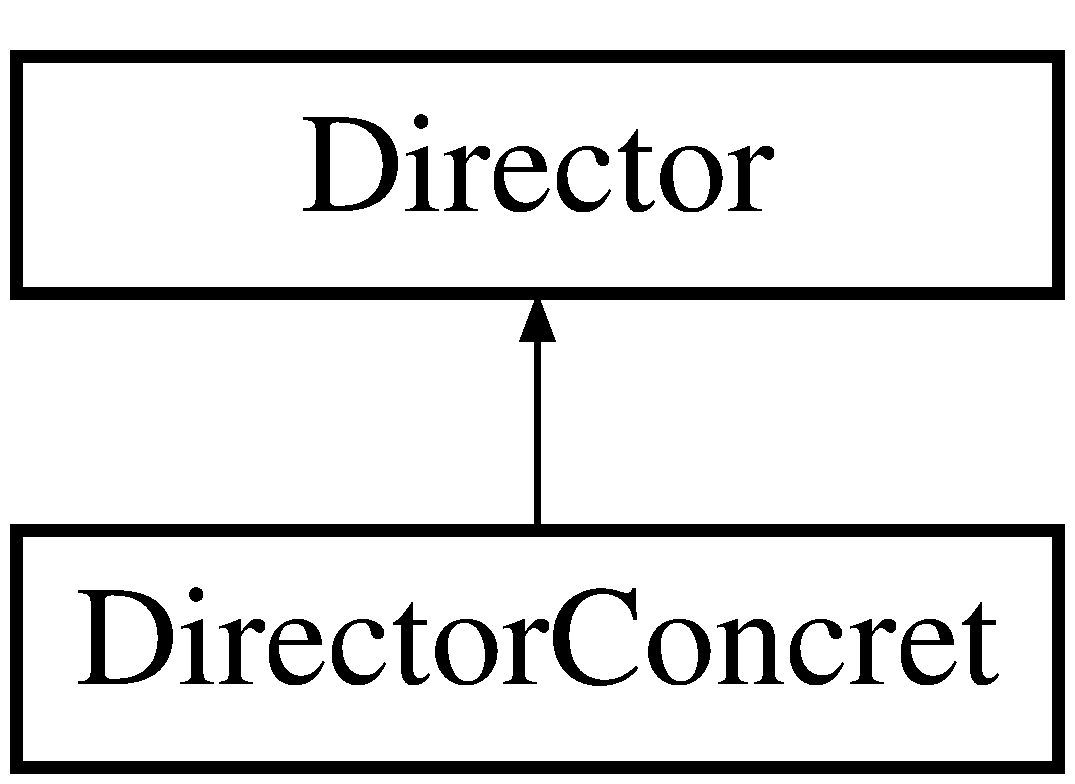
\includegraphics[height=2.000000cm]{class_director}
\end{center}
\end{figure}
\subsection*{Fonctions membres publiques}
\begin{DoxyCompactItemize}
\item 
virtual \hyperlink{class_deck}{Deck} $\ast$ \hyperlink{class_director_aea0cbfa1badb2688676406bf47fc7b62}{faire\-Deck} ()=0
\begin{DoxyCompactList}\small\item\em Permet de construire un deck à partir d'un fichier. \end{DoxyCompactList}\end{DoxyCompactItemize}
\subsection*{Attributs protégés}
\begin{DoxyCompactItemize}
\item 
\hyperlink{class_builder_deck}{Builder\-Deck} $\ast$ \hyperlink{class_director_aab69d1e289d61bf63407e8c1554a0c09}{builderdeck\-\_\-}
\end{DoxyCompactItemize}


\subsection{Description détaillée}
Classe \hyperlink{class_director}{Director} qui sert à gerer les builder de carte. 

\begin{DoxyDate}{Date}
15/11/2015 
\end{DoxyDate}
\begin{DoxyAuthor}{Auteur}
paul\-\_\-figiel 
\end{DoxyAuthor}


\subsection{Documentation des fonctions membres}
\hypertarget{class_director_aea0cbfa1badb2688676406bf47fc7b62}{\index{Director@{Director}!faire\-Deck@{faire\-Deck}}
\index{faire\-Deck@{faire\-Deck}!Director@{Director}}
\subsubsection[{faire\-Deck}]{\setlength{\rightskip}{0pt plus 5cm}virtual {\bf Deck}$\ast$ Director\-::faire\-Deck (
\begin{DoxyParamCaption}
{}
\end{DoxyParamCaption}
)\hspace{0.3cm}{\ttfamily [pure virtual]}}}\label{class_director_aea0cbfa1badb2688676406bf47fc7b62}


Permet de construire un deck à partir d'un fichier. 

\begin{DoxyReturn}{Renvoie}
\-: un pointeur sur le deck créé 
\end{DoxyReturn}


Implémenté dans \hyperlink{class_director_concret_a282099b6194ce102102b780a5b4bcb46}{Director\-Concret}.



\subsection{Documentation des données membres}
\hypertarget{class_director_aab69d1e289d61bf63407e8c1554a0c09}{\index{Director@{Director}!builderdeck\-\_\-@{builderdeck\-\_\-}}
\index{builderdeck\-\_\-@{builderdeck\-\_\-}!Director@{Director}}
\subsubsection[{builderdeck\-\_\-}]{\setlength{\rightskip}{0pt plus 5cm}{\bf Builder\-Deck}$\ast$ Director\-::builderdeck\-\_\-\hspace{0.3cm}{\ttfamily [protected]}}}\label{class_director_aab69d1e289d61bf63407e8c1554a0c09}
Le builder qui créé les decks 

La documentation de cette classe a été générée à partir du fichier suivant \-:\begin{DoxyCompactItemize}
\item 
/home/figiel-\/paul/\-Bureau/\-Projet\-Poo/\-Projet\-P\-O\-O-\/\-A\-R\-A\-Y\-A-\/\-F\-I\-G\-I\-E\-L/include/\hyperlink{_director_8hpp}{Director.\-hpp}\end{DoxyCompactItemize}

\hypertarget{class_director_concret}{\section{Référence de la classe Director\-Concret}
\label{class_director_concret}\index{Director\-Concret@{Director\-Concret}}
}


Classe \hyperlink{class_director_concret}{Director\-Concret} qui sert à gerer les builder de carte, implemente \hyperlink{class_director}{Director}.  




{\ttfamily \#include $<$Director\-Concret.\-hpp$>$}

Graphe d'héritage de Director\-Concret\-:\begin{figure}[H]
\begin{center}
\leavevmode
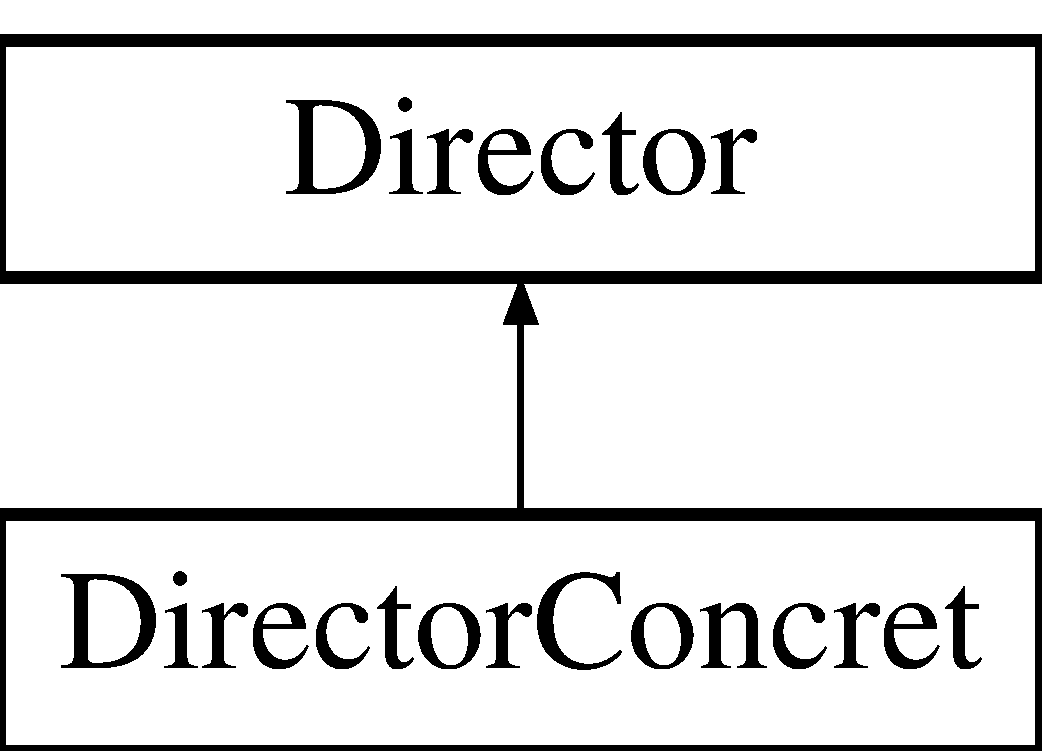
\includegraphics[height=2.000000cm]{class_director_concret}
\end{center}
\end{figure}
\subsection*{Fonctions membres publiques}
\begin{DoxyCompactItemize}
\item 
\hyperlink{class_director_concret_a08b1584ddf77a3b262458f144e23b699}{Director\-Concret} (\hyperlink{class_builder_deck}{Builder\-Deck} $\ast$bd)
\begin{DoxyCompactList}\small\item\em Constructeur. \end{DoxyCompactList}\item 
\hyperlink{class_deck}{Deck} $\ast$ \hyperlink{class_director_concret_a282099b6194ce102102b780a5b4bcb46}{faire\-Deck} ()
\begin{DoxyCompactList}\small\item\em Permet de construire un deck à partir d'un fichier. \end{DoxyCompactList}\end{DoxyCompactItemize}
\subsection*{Membres hérités additionnels}


\subsection{Description détaillée}
Classe \hyperlink{class_director_concret}{Director\-Concret} qui sert à gerer les builder de carte, implemente \hyperlink{class_director}{Director}. 

\begin{DoxyDate}{Date}
15/11/2015 
\end{DoxyDate}
\begin{DoxyAuthor}{Auteur}
paul\-\_\-figiel 
\end{DoxyAuthor}


\subsection{Documentation des constructeurs et destructeur}
\hypertarget{class_director_concret_a08b1584ddf77a3b262458f144e23b699}{\index{Director\-Concret@{Director\-Concret}!Director\-Concret@{Director\-Concret}}
\index{Director\-Concret@{Director\-Concret}!DirectorConcret@{Director\-Concret}}
\subsubsection[{Director\-Concret}]{\setlength{\rightskip}{0pt plus 5cm}Director\-Concret\-::\-Director\-Concret (
\begin{DoxyParamCaption}
\item[{{\bf Builder\-Deck} $\ast$}]{bd}
\end{DoxyParamCaption}
)\hspace{0.3cm}{\ttfamily [inline]}}}\label{class_director_concret_a08b1584ddf77a3b262458f144e23b699}


Constructeur. 

Constructeur de la classe \hyperlink{class_director_concret}{Director\-Concret}


\begin{DoxyParams}{Paramètres}
{\em bd} & \-: le builder que doit gerer le director \\
\hline
\end{DoxyParams}


\subsection{Documentation des fonctions membres}
\hypertarget{class_director_concret_a282099b6194ce102102b780a5b4bcb46}{\index{Director\-Concret@{Director\-Concret}!faire\-Deck@{faire\-Deck}}
\index{faire\-Deck@{faire\-Deck}!DirectorConcret@{Director\-Concret}}
\subsubsection[{faire\-Deck}]{\setlength{\rightskip}{0pt plus 5cm}{\bf Deck}$\ast$ Director\-Concret\-::faire\-Deck (
\begin{DoxyParamCaption}
{}
\end{DoxyParamCaption}
)\hspace{0.3cm}{\ttfamily [virtual]}}}\label{class_director_concret_a282099b6194ce102102b780a5b4bcb46}


Permet de construire un deck à partir d'un fichier. 

\begin{DoxyReturn}{Renvoie}
\-: un pointeur sur le deck créé 
\end{DoxyReturn}


Implémente \hyperlink{class_director_aea0cbfa1badb2688676406bf47fc7b62}{Director}.



La documentation de cette classe a été générée à partir du fichier suivant \-:\begin{DoxyCompactItemize}
\item 
/home/figiel-\/paul/\-Bureau/\-Projet\-Poo/\-Projet\-P\-O\-O-\/\-A\-R\-A\-Y\-A-\/\-F\-I\-G\-I\-E\-L/include/\hyperlink{_director_concret_8hpp}{Director\-Concret.\-hpp}\end{DoxyCompactItemize}

\hypertarget{class_effet}{\section{Référence de la classe Effet}
\label{class_effet}\index{Effet@{Effet}}
}


{\ttfamily \#include $<$Effet.\-hpp$>$}

Graphe d'héritage de Effet\-:\begin{figure}[H]
\begin{center}
\leavevmode
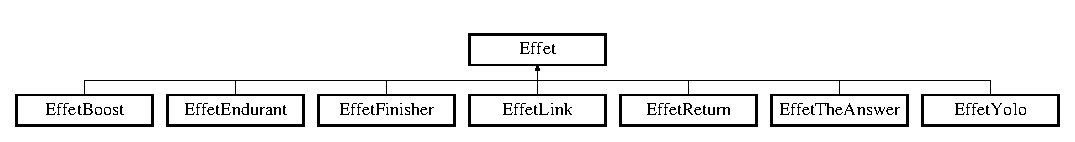
\includegraphics[height=1.454545cm]{class_effet}
\end{center}
\end{figure}
\subsection*{Fonctions membres publiques}
\begin{DoxyCompactItemize}
\item 
\hyperlink{class_effet_a79744b45fc5715a4742e63565d4f89cb}{Effet} ()
\begin{DoxyCompactList}\small\item\em Constructeur vide. \end{DoxyCompactList}\item 
virtual void \hyperlink{class_effet_a57adb1db82d03cda90600f93cc8b5197}{action\-Effet} (\hyperlink{class_jeu}{Jeu} $\ast$jeu, int x)
\begin{DoxyCompactList}\small\item\em applique l'effet \end{DoxyCompactList}\item 
virtual void \hyperlink{class_effet_a1bc485c64cfa136e279d5c9183b3e41d}{afficher} ()=0
\begin{DoxyCompactList}\small\item\em affiche le nom de l'effet et ce qu'il fait \end{DoxyCompactList}\item 
virtual std\-::string \hyperlink{class_effet_a1d3b1a8092df2624399c80d24a21cc88}{get\-Nom} ()=0
\begin{DoxyCompactList}\small\item\em va chercher le nom de l'effet \end{DoxyCompactList}\end{DoxyCompactItemize}


\subsection{Documentation des constructeurs et destructeur}
\hypertarget{class_effet_a79744b45fc5715a4742e63565d4f89cb}{\index{Effet@{Effet}!Effet@{Effet}}
\index{Effet@{Effet}!Effet@{Effet}}
\subsubsection[{Effet}]{\setlength{\rightskip}{0pt plus 5cm}Effet\-::\-Effet (
\begin{DoxyParamCaption}
{}
\end{DoxyParamCaption}
)\hspace{0.3cm}{\ttfamily [inline]}}}\label{class_effet_a79744b45fc5715a4742e63565d4f89cb}


Constructeur vide. 

Constructeur de la classe \hyperlink{class_effet}{Effet} 

\subsection{Documentation des fonctions membres}
\hypertarget{class_effet_a57adb1db82d03cda90600f93cc8b5197}{\index{Effet@{Effet}!action\-Effet@{action\-Effet}}
\index{action\-Effet@{action\-Effet}!Effet@{Effet}}
\subsubsection[{action\-Effet}]{\setlength{\rightskip}{0pt plus 5cm}virtual void Effet\-::action\-Effet (
\begin{DoxyParamCaption}
\item[{{\bf Jeu} $\ast$}]{jeu, }
\item[{int}]{x}
\end{DoxyParamCaption}
)\hspace{0.3cm}{\ttfamily [inline]}, {\ttfamily [virtual]}}}\label{class_effet_a57adb1db82d03cda90600f93cc8b5197}


applique l'effet 


\begin{DoxyParams}{Paramètres}
{\em \hyperlink{class_jeu}{Jeu}} & $\ast$jeu \-: le jeu \\
\hline
{\em int} & x \-: le joueur qui joue l'effet \\
\hline
\end{DoxyParams}


Réimplémentée dans \hyperlink{class_effet_boost_a8584fa1a61d87ffd7ec51782b78413c4}{Effet\-Boost}, \hyperlink{class_effet_endurant_affdc8528f7315776243ae2b08523dda2}{Effet\-Endurant}, \hyperlink{class_effet_the_answer_a3e8f2cad127fdf393f1421eb04a6ebe8}{Effet\-The\-Answer}, \hyperlink{class_effet_finisher_ab0980df9cf22d096c61c5acc90ddeb43}{Effet\-Finisher}, \hyperlink{class_effet_link_a92936d48d1685122199da60317e6199a}{Effet\-Link}, \hyperlink{class_effet_return_a9bd08ea82f466e0a0181a83cd1922a52}{Effet\-Return}, et \hyperlink{class_effet_yolo_abb0ba5ceef4b948c833519557c850cf3}{Effet\-Yolo}.

\hypertarget{class_effet_a1bc485c64cfa136e279d5c9183b3e41d}{\index{Effet@{Effet}!afficher@{afficher}}
\index{afficher@{afficher}!Effet@{Effet}}
\subsubsection[{afficher}]{\setlength{\rightskip}{0pt plus 5cm}virtual void Effet\-::afficher (
\begin{DoxyParamCaption}
{}
\end{DoxyParamCaption}
)\hspace{0.3cm}{\ttfamily [pure virtual]}}}\label{class_effet_a1bc485c64cfa136e279d5c9183b3e41d}


affiche le nom de l'effet et ce qu'il fait 



Implémenté dans \hyperlink{class_effet_boost_a5cd27853b4b1dd08ff0c7465f5890bf4}{Effet\-Boost}, \hyperlink{class_effet_endurant_a41b08a28984aaa91d07331731ea57a80}{Effet\-Endurant}, \hyperlink{class_effet_the_answer_a35ba2f942b38ffc60c9c64a763ba77b5}{Effet\-The\-Answer}, \hyperlink{class_effet_finisher_ae6a5994848a870f415bf2aacc5377109}{Effet\-Finisher}, \hyperlink{class_effet_link_a3d02ae47a14a579bd9582b744d4307d7}{Effet\-Link}, \hyperlink{class_effet_return_aeb7b436619ff6654961fd421c1886be8}{Effet\-Return}, et \hyperlink{class_effet_yolo_afd45910743596b404709e5da05a507bb}{Effet\-Yolo}.

\hypertarget{class_effet_a1d3b1a8092df2624399c80d24a21cc88}{\index{Effet@{Effet}!get\-Nom@{get\-Nom}}
\index{get\-Nom@{get\-Nom}!Effet@{Effet}}
\subsubsection[{get\-Nom}]{\setlength{\rightskip}{0pt plus 5cm}virtual std\-::string Effet\-::get\-Nom (
\begin{DoxyParamCaption}
{}
\end{DoxyParamCaption}
)\hspace{0.3cm}{\ttfamily [pure virtual]}}}\label{class_effet_a1d3b1a8092df2624399c80d24a21cc88}


va chercher le nom de l'effet 

\begin{DoxyReturn}{Renvoie}
\-: une string qui corespond au nom de l'effet' 
\end{DoxyReturn}


Implémenté dans \hyperlink{class_effet_boost_aba325a637c5e0bb4bea74179ae27ea69}{Effet\-Boost}, \hyperlink{class_effet_endurant_adc7d05da5bcdd44cb5623420c5b67bf5}{Effet\-Endurant}, \hyperlink{class_effet_the_answer_a4438775df11e19a34226ac8f8b499961}{Effet\-The\-Answer}, \hyperlink{class_effet_finisher_a86281252a8294c6398602e5dcd956ad9}{Effet\-Finisher}, \hyperlink{class_effet_link_a3c5e55a3e756a3c012c9c9643f5747a2}{Effet\-Link}, \hyperlink{class_effet_return_ad8ac1f6ec29d8472a06d0d4d22e5ad8d}{Effet\-Return}, et \hyperlink{class_effet_yolo_a1118497023e66bc661aca8ba4189f036}{Effet\-Yolo}.



La documentation de cette classe a été générée à partir du fichier suivant \-:\begin{DoxyCompactItemize}
\item 
/home/figiel-\/paul/\-Bureau/\-Projet\-Poo/\-Projet\-P\-O\-O-\/\-A\-R\-A\-Y\-A-\/\-F\-I\-G\-I\-E\-L/include/\hyperlink{_effet_8hpp}{Effet.\-hpp}\end{DoxyCompactItemize}

\hypertarget{class_effet_boost}{\section{Référence de la classe Effet\-Boost}
\label{class_effet_boost}\index{Effet\-Boost@{Effet\-Boost}}
}


{\ttfamily \#include $<$Effet\-Boost.\-hpp$>$}

Graphe d'héritage de Effet\-Boost\-:\begin{figure}[H]
\begin{center}
\leavevmode
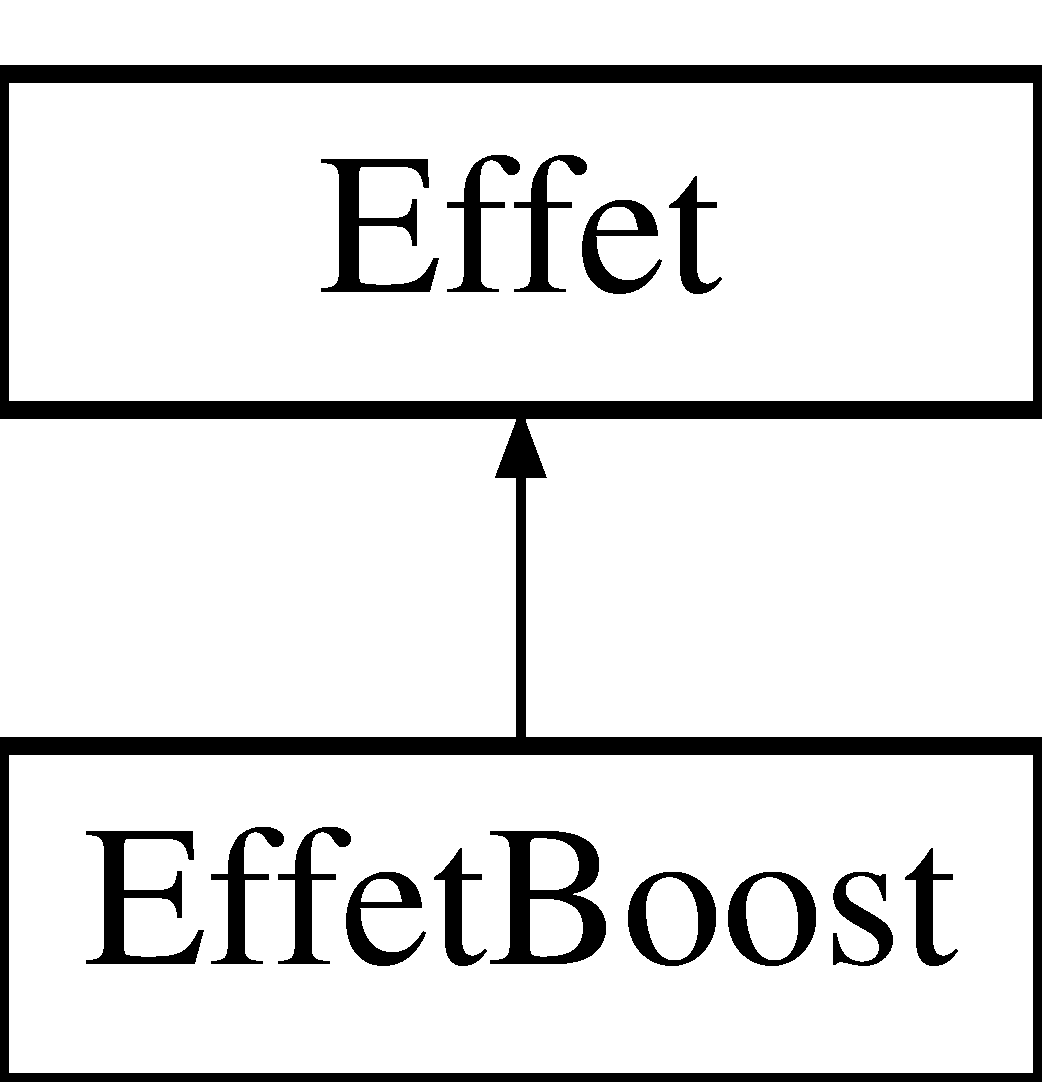
\includegraphics[height=2.000000cm]{class_effet_boost}
\end{center}
\end{figure}
\subsection*{Fonctions membres publiques}
\begin{DoxyCompactItemize}
\item 
\hyperlink{class_effet_boost_a04a8c134416d167152558826efbead82}{Effet\-Boost} ()
\item 
void \hyperlink{class_effet_boost_a8584fa1a61d87ffd7ec51782b78413c4}{action\-Effet} (\hyperlink{class_jeu}{Jeu} $\ast$jeu, int x)
\begin{DoxyCompactList}\small\item\em applique l'effet \end{DoxyCompactList}\item 
void \hyperlink{class_effet_boost_a5cd27853b4b1dd08ff0c7465f5890bf4}{afficher} ()
\begin{DoxyCompactList}\small\item\em affiche le nom de l'effet et ce qu'il fait \end{DoxyCompactList}\item 
std\-::string \hyperlink{class_effet_boost_aba325a637c5e0bb4bea74179ae27ea69}{get\-Nom} ()
\begin{DoxyCompactList}\small\item\em va chercher le nom de l'effet \end{DoxyCompactList}\end{DoxyCompactItemize}


\subsection{Documentation des constructeurs et destructeur}
\hypertarget{class_effet_boost_a04a8c134416d167152558826efbead82}{\index{Effet\-Boost@{Effet\-Boost}!Effet\-Boost@{Effet\-Boost}}
\index{Effet\-Boost@{Effet\-Boost}!EffetBoost@{Effet\-Boost}}
\subsubsection[{Effet\-Boost}]{\setlength{\rightskip}{0pt plus 5cm}Effet\-Boost\-::\-Effet\-Boost (
\begin{DoxyParamCaption}
{}
\end{DoxyParamCaption}
)\hspace{0.3cm}{\ttfamily [inline]}}}\label{class_effet_boost_a04a8c134416d167152558826efbead82}


\subsection{Documentation des fonctions membres}
\hypertarget{class_effet_boost_a8584fa1a61d87ffd7ec51782b78413c4}{\index{Effet\-Boost@{Effet\-Boost}!action\-Effet@{action\-Effet}}
\index{action\-Effet@{action\-Effet}!EffetBoost@{Effet\-Boost}}
\subsubsection[{action\-Effet}]{\setlength{\rightskip}{0pt plus 5cm}void Effet\-Boost\-::action\-Effet (
\begin{DoxyParamCaption}
\item[{{\bf Jeu} $\ast$}]{jeu, }
\item[{int}]{x}
\end{DoxyParamCaption}
)\hspace{0.3cm}{\ttfamily [virtual]}}}\label{class_effet_boost_a8584fa1a61d87ffd7ec51782b78413c4}


applique l'effet 


\begin{DoxyParams}{Paramètres}
{\em \hyperlink{class_jeu}{Jeu}} & $\ast$jeu \-: le jeu \\
\hline
{\em int} & x \-: le joueur qui joue l'effet \\
\hline
\end{DoxyParams}


Réimplémentée à partir de \hyperlink{class_effet_a57adb1db82d03cda90600f93cc8b5197}{Effet}.

\hypertarget{class_effet_boost_a5cd27853b4b1dd08ff0c7465f5890bf4}{\index{Effet\-Boost@{Effet\-Boost}!afficher@{afficher}}
\index{afficher@{afficher}!EffetBoost@{Effet\-Boost}}
\subsubsection[{afficher}]{\setlength{\rightskip}{0pt plus 5cm}void Effet\-Boost\-::afficher (
\begin{DoxyParamCaption}
{}
\end{DoxyParamCaption}
)\hspace{0.3cm}{\ttfamily [virtual]}}}\label{class_effet_boost_a5cd27853b4b1dd08ff0c7465f5890bf4}


affiche le nom de l'effet et ce qu'il fait 



Implémente \hyperlink{class_effet_a1bc485c64cfa136e279d5c9183b3e41d}{Effet}.

\hypertarget{class_effet_boost_aba325a637c5e0bb4bea74179ae27ea69}{\index{Effet\-Boost@{Effet\-Boost}!get\-Nom@{get\-Nom}}
\index{get\-Nom@{get\-Nom}!EffetBoost@{Effet\-Boost}}
\subsubsection[{get\-Nom}]{\setlength{\rightskip}{0pt plus 5cm}std\-::string Effet\-Boost\-::get\-Nom (
\begin{DoxyParamCaption}
{}
\end{DoxyParamCaption}
)\hspace{0.3cm}{\ttfamily [virtual]}}}\label{class_effet_boost_aba325a637c5e0bb4bea74179ae27ea69}


va chercher le nom de l'effet 

\begin{DoxyReturn}{Renvoie}
\-: une string qui corespond au nom de l'effet' 
\end{DoxyReturn}


Implémente \hyperlink{class_effet_a1d3b1a8092df2624399c80d24a21cc88}{Effet}.



La documentation de cette classe a été générée à partir du fichier suivant \-:\begin{DoxyCompactItemize}
\item 
/home/figiel-\/paul/\-Bureau/\-Projet\-Poo/\-Projet\-P\-O\-O-\/\-A\-R\-A\-Y\-A-\/\-F\-I\-G\-I\-E\-L/include/\hyperlink{_effet_boost_8hpp}{Effet\-Boost.\-hpp}\end{DoxyCompactItemize}

\hypertarget{class_effet_endurant}{\section{Référence de la classe Effet\-Endurant}
\label{class_effet_endurant}\index{Effet\-Endurant@{Effet\-Endurant}}
}


{\ttfamily \#include $<$Effet\-Endurant.\-hpp$>$}

Graphe d'héritage de Effet\-Endurant\-:\begin{figure}[H]
\begin{center}
\leavevmode
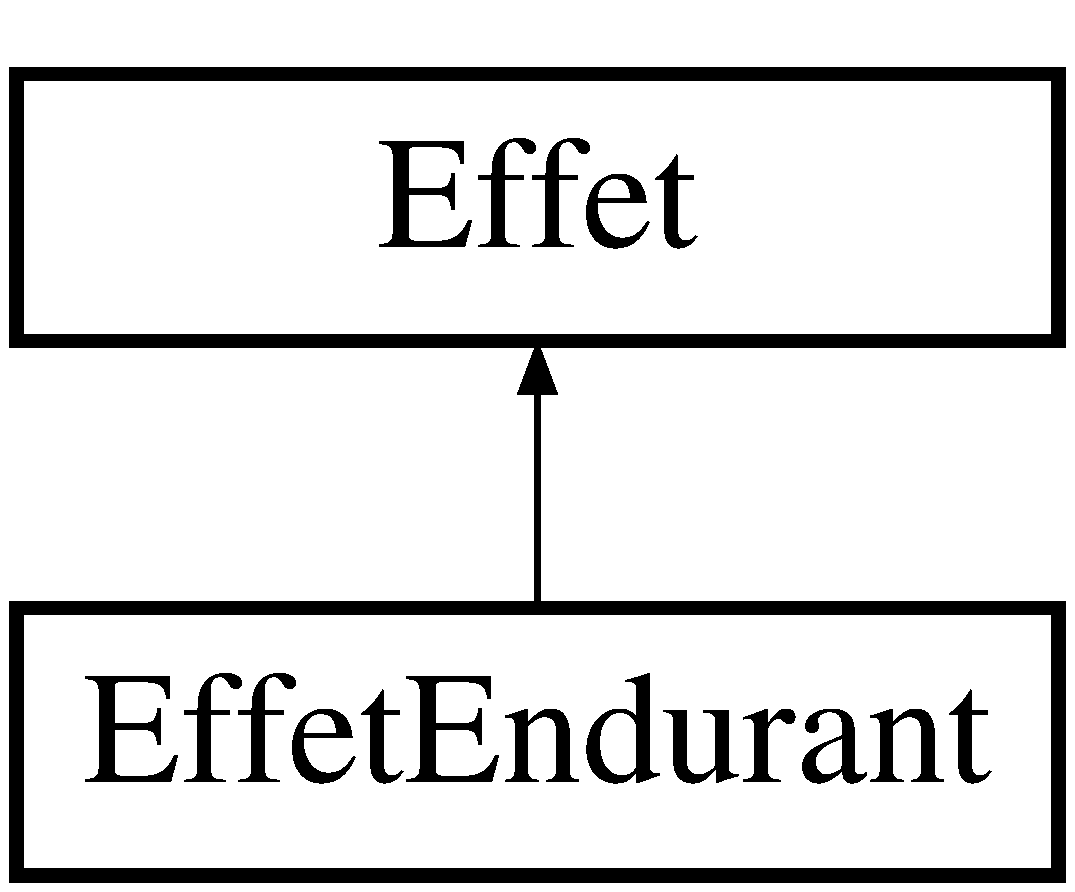
\includegraphics[height=2.000000cm]{class_effet_endurant}
\end{center}
\end{figure}
\subsection*{Fonctions membres publiques}
\begin{DoxyCompactItemize}
\item 
\hyperlink{class_effet_endurant_a76fa08e1045499c3659dce9192f08e14}{Effet\-Endurant} ()
\item 
void \hyperlink{class_effet_endurant_affdc8528f7315776243ae2b08523dda2}{action\-Effet} (\hyperlink{class_jeu}{Jeu} $\ast$jeu, int x)
\begin{DoxyCompactList}\small\item\em applique l'effet \end{DoxyCompactList}\item 
void \hyperlink{class_effet_endurant_a41b08a28984aaa91d07331731ea57a80}{afficher} ()
\begin{DoxyCompactList}\small\item\em affiche le nom de l'effet et ce qu'il fait \end{DoxyCompactList}\item 
std\-::string \hyperlink{class_effet_endurant_adc7d05da5bcdd44cb5623420c5b67bf5}{get\-Nom} ()
\begin{DoxyCompactList}\small\item\em va chercher le nom de l'effet \end{DoxyCompactList}\end{DoxyCompactItemize}


\subsection{Documentation des constructeurs et destructeur}
\hypertarget{class_effet_endurant_a76fa08e1045499c3659dce9192f08e14}{\index{Effet\-Endurant@{Effet\-Endurant}!Effet\-Endurant@{Effet\-Endurant}}
\index{Effet\-Endurant@{Effet\-Endurant}!EffetEndurant@{Effet\-Endurant}}
\subsubsection[{Effet\-Endurant}]{\setlength{\rightskip}{0pt plus 5cm}Effet\-Endurant\-::\-Effet\-Endurant (
\begin{DoxyParamCaption}
{}
\end{DoxyParamCaption}
)\hspace{0.3cm}{\ttfamily [inline]}}}\label{class_effet_endurant_a76fa08e1045499c3659dce9192f08e14}


\subsection{Documentation des fonctions membres}
\hypertarget{class_effet_endurant_affdc8528f7315776243ae2b08523dda2}{\index{Effet\-Endurant@{Effet\-Endurant}!action\-Effet@{action\-Effet}}
\index{action\-Effet@{action\-Effet}!EffetEndurant@{Effet\-Endurant}}
\subsubsection[{action\-Effet}]{\setlength{\rightskip}{0pt plus 5cm}void Effet\-Endurant\-::action\-Effet (
\begin{DoxyParamCaption}
\item[{{\bf Jeu} $\ast$}]{jeu, }
\item[{int}]{x}
\end{DoxyParamCaption}
)\hspace{0.3cm}{\ttfamily [virtual]}}}\label{class_effet_endurant_affdc8528f7315776243ae2b08523dda2}


applique l'effet 


\begin{DoxyParams}{Paramètres}
{\em \hyperlink{class_jeu}{Jeu}} & $\ast$jeu \-: le jeu \\
\hline
{\em int} & x \-: le joueur qui joue l'effet \\
\hline
\end{DoxyParams}


Réimplémentée à partir de \hyperlink{class_effet_a57adb1db82d03cda90600f93cc8b5197}{Effet}.

\hypertarget{class_effet_endurant_a41b08a28984aaa91d07331731ea57a80}{\index{Effet\-Endurant@{Effet\-Endurant}!afficher@{afficher}}
\index{afficher@{afficher}!EffetEndurant@{Effet\-Endurant}}
\subsubsection[{afficher}]{\setlength{\rightskip}{0pt plus 5cm}void Effet\-Endurant\-::afficher (
\begin{DoxyParamCaption}
{}
\end{DoxyParamCaption}
)\hspace{0.3cm}{\ttfamily [virtual]}}}\label{class_effet_endurant_a41b08a28984aaa91d07331731ea57a80}


affiche le nom de l'effet et ce qu'il fait 



Implémente \hyperlink{class_effet_a1bc485c64cfa136e279d5c9183b3e41d}{Effet}.

\hypertarget{class_effet_endurant_adc7d05da5bcdd44cb5623420c5b67bf5}{\index{Effet\-Endurant@{Effet\-Endurant}!get\-Nom@{get\-Nom}}
\index{get\-Nom@{get\-Nom}!EffetEndurant@{Effet\-Endurant}}
\subsubsection[{get\-Nom}]{\setlength{\rightskip}{0pt plus 5cm}std\-::string Effet\-Endurant\-::get\-Nom (
\begin{DoxyParamCaption}
{}
\end{DoxyParamCaption}
)\hspace{0.3cm}{\ttfamily [virtual]}}}\label{class_effet_endurant_adc7d05da5bcdd44cb5623420c5b67bf5}


va chercher le nom de l'effet 

\begin{DoxyReturn}{Renvoie}
\-: une string qui corespond au nom de l'effet' 
\end{DoxyReturn}


Implémente \hyperlink{class_effet_a1d3b1a8092df2624399c80d24a21cc88}{Effet}.



La documentation de cette classe a été générée à partir du fichier suivant \-:\begin{DoxyCompactItemize}
\item 
/home/figiel-\/paul/\-Bureau/\-Projet\-Poo/\-Projet\-P\-O\-O-\/\-A\-R\-A\-Y\-A-\/\-F\-I\-G\-I\-E\-L/include/\hyperlink{_effet_endurant_8hpp}{Effet\-Endurant.\-hpp}\end{DoxyCompactItemize}

\hypertarget{class_effet_finisher}{\section{Référence de la classe Effet\-Finisher}
\label{class_effet_finisher}\index{Effet\-Finisher@{Effet\-Finisher}}
}


{\ttfamily \#include $<$Effet\-Finisher.\-hpp$>$}

Graphe d'héritage de Effet\-Finisher\-:\begin{figure}[H]
\begin{center}
\leavevmode
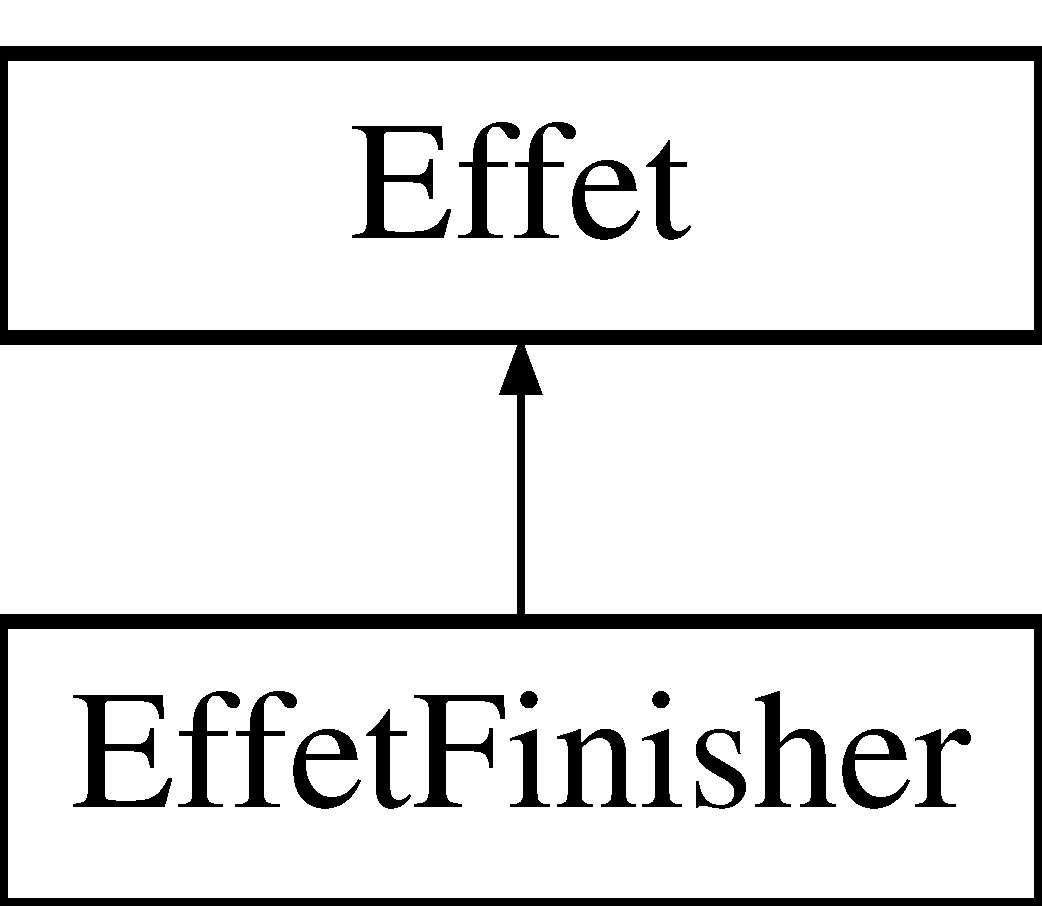
\includegraphics[height=2.000000cm]{class_effet_finisher}
\end{center}
\end{figure}
\subsection*{Fonctions membres publiques}
\begin{DoxyCompactItemize}
\item 
\hyperlink{class_effet_finisher_ac9ffcb6398a1c79c40d7ed43b4740389}{Effet\-Finisher} ()
\item 
void \hyperlink{class_effet_finisher_ab0980df9cf22d096c61c5acc90ddeb43}{action\-Effet} (\hyperlink{class_jeu}{Jeu} $\ast$jeu, int x)
\begin{DoxyCompactList}\small\item\em applique l'effet \end{DoxyCompactList}\item 
void \hyperlink{class_effet_finisher_ae6a5994848a870f415bf2aacc5377109}{afficher} ()
\begin{DoxyCompactList}\small\item\em affiche le nom de l'effet et ce qu'il fait \end{DoxyCompactList}\item 
std\-::string \hyperlink{class_effet_finisher_a86281252a8294c6398602e5dcd956ad9}{get\-Nom} ()
\begin{DoxyCompactList}\small\item\em va chercher le nom de l'effet \end{DoxyCompactList}\end{DoxyCompactItemize}


\subsection{Documentation des constructeurs et destructeur}
\hypertarget{class_effet_finisher_ac9ffcb6398a1c79c40d7ed43b4740389}{\index{Effet\-Finisher@{Effet\-Finisher}!Effet\-Finisher@{Effet\-Finisher}}
\index{Effet\-Finisher@{Effet\-Finisher}!EffetFinisher@{Effet\-Finisher}}
\subsubsection[{Effet\-Finisher}]{\setlength{\rightskip}{0pt plus 5cm}Effet\-Finisher\-::\-Effet\-Finisher (
\begin{DoxyParamCaption}
{}
\end{DoxyParamCaption}
)\hspace{0.3cm}{\ttfamily [inline]}}}\label{class_effet_finisher_ac9ffcb6398a1c79c40d7ed43b4740389}


\subsection{Documentation des fonctions membres}
\hypertarget{class_effet_finisher_ab0980df9cf22d096c61c5acc90ddeb43}{\index{Effet\-Finisher@{Effet\-Finisher}!action\-Effet@{action\-Effet}}
\index{action\-Effet@{action\-Effet}!EffetFinisher@{Effet\-Finisher}}
\subsubsection[{action\-Effet}]{\setlength{\rightskip}{0pt plus 5cm}void Effet\-Finisher\-::action\-Effet (
\begin{DoxyParamCaption}
\item[{{\bf Jeu} $\ast$}]{jeu, }
\item[{int}]{x}
\end{DoxyParamCaption}
)\hspace{0.3cm}{\ttfamily [virtual]}}}\label{class_effet_finisher_ab0980df9cf22d096c61c5acc90ddeb43}


applique l'effet 


\begin{DoxyParams}{Paramètres}
{\em \hyperlink{class_jeu}{Jeu}} & $\ast$jeu \-: le jeu \\
\hline
{\em int} & x \-: le joueur qui joue l'effet \\
\hline
\end{DoxyParams}


Réimplémentée à partir de \hyperlink{class_effet_a57adb1db82d03cda90600f93cc8b5197}{Effet}.

\hypertarget{class_effet_finisher_ae6a5994848a870f415bf2aacc5377109}{\index{Effet\-Finisher@{Effet\-Finisher}!afficher@{afficher}}
\index{afficher@{afficher}!EffetFinisher@{Effet\-Finisher}}
\subsubsection[{afficher}]{\setlength{\rightskip}{0pt plus 5cm}void Effet\-Finisher\-::afficher (
\begin{DoxyParamCaption}
{}
\end{DoxyParamCaption}
)\hspace{0.3cm}{\ttfamily [virtual]}}}\label{class_effet_finisher_ae6a5994848a870f415bf2aacc5377109}


affiche le nom de l'effet et ce qu'il fait 



Implémente \hyperlink{class_effet_a1bc485c64cfa136e279d5c9183b3e41d}{Effet}.

\hypertarget{class_effet_finisher_a86281252a8294c6398602e5dcd956ad9}{\index{Effet\-Finisher@{Effet\-Finisher}!get\-Nom@{get\-Nom}}
\index{get\-Nom@{get\-Nom}!EffetFinisher@{Effet\-Finisher}}
\subsubsection[{get\-Nom}]{\setlength{\rightskip}{0pt plus 5cm}std\-::string Effet\-Finisher\-::get\-Nom (
\begin{DoxyParamCaption}
{}
\end{DoxyParamCaption}
)\hspace{0.3cm}{\ttfamily [virtual]}}}\label{class_effet_finisher_a86281252a8294c6398602e5dcd956ad9}


va chercher le nom de l'effet 

\begin{DoxyReturn}{Renvoie}
\-: une string qui corespond au nom de l'effet' 
\end{DoxyReturn}


Implémente \hyperlink{class_effet_a1d3b1a8092df2624399c80d24a21cc88}{Effet}.



La documentation de cette classe a été générée à partir du fichier suivant \-:\begin{DoxyCompactItemize}
\item 
/home/figiel-\/paul/\-Bureau/\-Projet\-Poo/\-Projet\-P\-O\-O-\/\-A\-R\-A\-Y\-A-\/\-F\-I\-G\-I\-E\-L/include/\hyperlink{_effet_finisher_8hpp}{Effet\-Finisher.\-hpp}\end{DoxyCompactItemize}

\hypertarget{class_effet_link}{\section{Référence de la classe Effet\-Link}
\label{class_effet_link}\index{Effet\-Link@{Effet\-Link}}
}


{\ttfamily \#include $<$Effet\-Link.\-hpp$>$}

Graphe d'héritage de Effet\-Link\-:\begin{figure}[H]
\begin{center}
\leavevmode
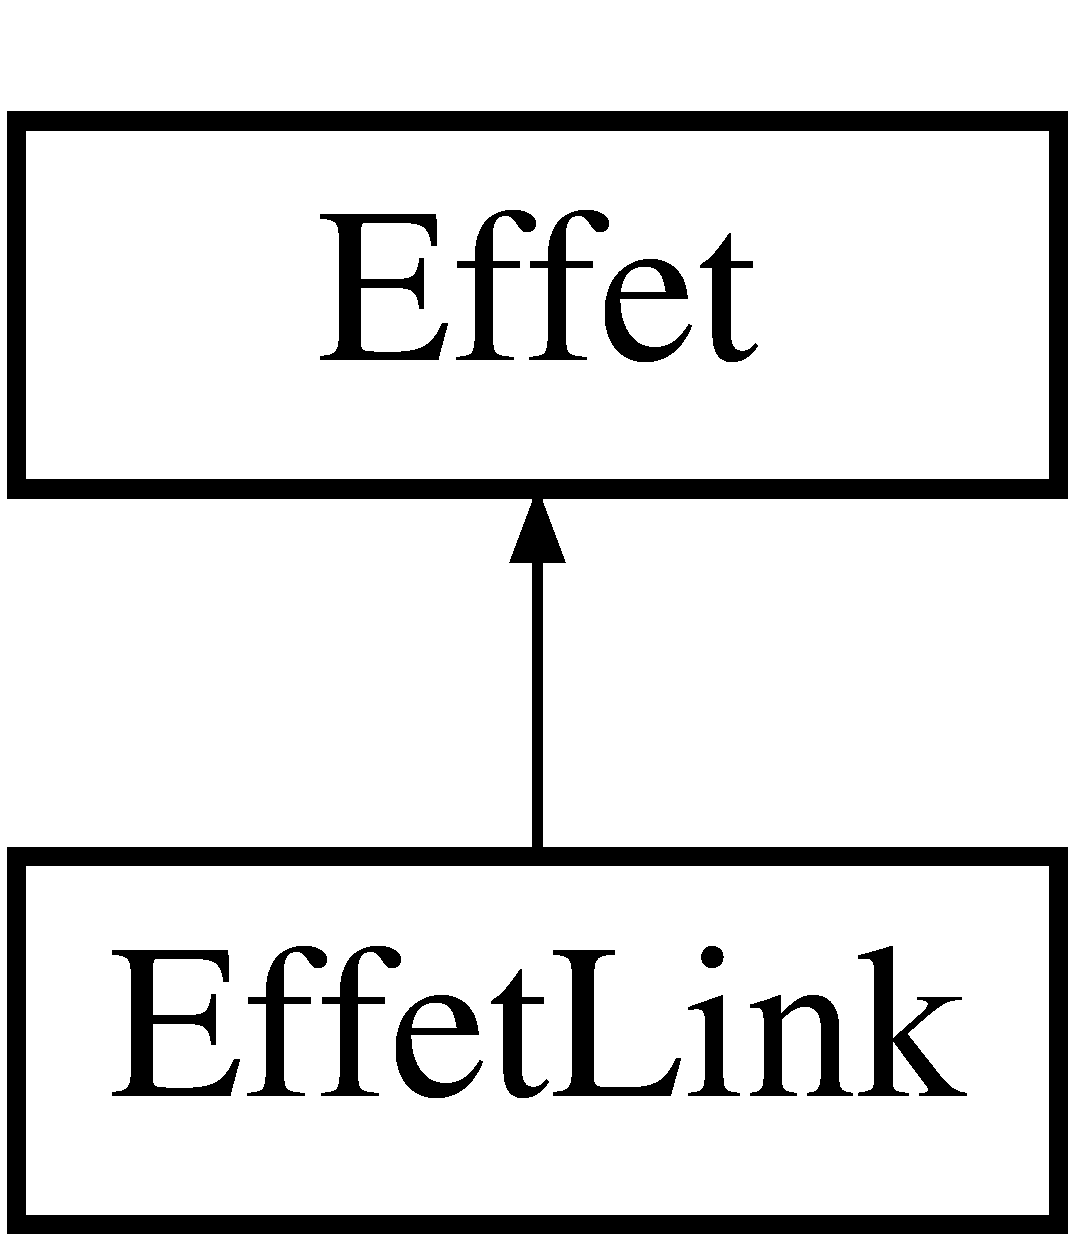
\includegraphics[height=2.000000cm]{class_effet_link}
\end{center}
\end{figure}
\subsection*{Fonctions membres publiques}
\begin{DoxyCompactItemize}
\item 
\hyperlink{class_effet_link_a744d555e2f195421e05a028746ba1a36}{Effet\-Link} ()
\item 
void \hyperlink{class_effet_link_a92936d48d1685122199da60317e6199a}{action\-Effet} (\hyperlink{class_jeu}{Jeu} $\ast$jeu, int x)
\begin{DoxyCompactList}\small\item\em applique l'effet \end{DoxyCompactList}\item 
void \hyperlink{class_effet_link_a3d02ae47a14a579bd9582b744d4307d7}{afficher} ()
\begin{DoxyCompactList}\small\item\em affiche le nom de l'effet et ce qu'il fait \end{DoxyCompactList}\item 
std\-::string \hyperlink{class_effet_link_a3c5e55a3e756a3c012c9c9643f5747a2}{get\-Nom} ()
\begin{DoxyCompactList}\small\item\em va chercher le nom de l'effet \end{DoxyCompactList}\end{DoxyCompactItemize}


\subsection{Documentation des constructeurs et destructeur}
\hypertarget{class_effet_link_a744d555e2f195421e05a028746ba1a36}{\index{Effet\-Link@{Effet\-Link}!Effet\-Link@{Effet\-Link}}
\index{Effet\-Link@{Effet\-Link}!EffetLink@{Effet\-Link}}
\subsubsection[{Effet\-Link}]{\setlength{\rightskip}{0pt plus 5cm}Effet\-Link\-::\-Effet\-Link (
\begin{DoxyParamCaption}
{}
\end{DoxyParamCaption}
)\hspace{0.3cm}{\ttfamily [inline]}}}\label{class_effet_link_a744d555e2f195421e05a028746ba1a36}


\subsection{Documentation des fonctions membres}
\hypertarget{class_effet_link_a92936d48d1685122199da60317e6199a}{\index{Effet\-Link@{Effet\-Link}!action\-Effet@{action\-Effet}}
\index{action\-Effet@{action\-Effet}!EffetLink@{Effet\-Link}}
\subsubsection[{action\-Effet}]{\setlength{\rightskip}{0pt plus 5cm}void Effet\-Link\-::action\-Effet (
\begin{DoxyParamCaption}
\item[{{\bf Jeu} $\ast$}]{jeu, }
\item[{int}]{x}
\end{DoxyParamCaption}
)\hspace{0.3cm}{\ttfamily [virtual]}}}\label{class_effet_link_a92936d48d1685122199da60317e6199a}


applique l'effet 


\begin{DoxyParams}{Paramètres}
{\em \hyperlink{class_jeu}{Jeu}} & $\ast$jeu \-: le jeu \\
\hline
{\em int} & x \-: le joueur qui joue l'effet \\
\hline
\end{DoxyParams}


Réimplémentée à partir de \hyperlink{class_effet_a57adb1db82d03cda90600f93cc8b5197}{Effet}.

\hypertarget{class_effet_link_a3d02ae47a14a579bd9582b744d4307d7}{\index{Effet\-Link@{Effet\-Link}!afficher@{afficher}}
\index{afficher@{afficher}!EffetLink@{Effet\-Link}}
\subsubsection[{afficher}]{\setlength{\rightskip}{0pt plus 5cm}void Effet\-Link\-::afficher (
\begin{DoxyParamCaption}
{}
\end{DoxyParamCaption}
)\hspace{0.3cm}{\ttfamily [virtual]}}}\label{class_effet_link_a3d02ae47a14a579bd9582b744d4307d7}


affiche le nom de l'effet et ce qu'il fait 



Implémente \hyperlink{class_effet_a1bc485c64cfa136e279d5c9183b3e41d}{Effet}.

\hypertarget{class_effet_link_a3c5e55a3e756a3c012c9c9643f5747a2}{\index{Effet\-Link@{Effet\-Link}!get\-Nom@{get\-Nom}}
\index{get\-Nom@{get\-Nom}!EffetLink@{Effet\-Link}}
\subsubsection[{get\-Nom}]{\setlength{\rightskip}{0pt plus 5cm}std\-::string Effet\-Link\-::get\-Nom (
\begin{DoxyParamCaption}
{}
\end{DoxyParamCaption}
)\hspace{0.3cm}{\ttfamily [virtual]}}}\label{class_effet_link_a3c5e55a3e756a3c012c9c9643f5747a2}


va chercher le nom de l'effet 

\begin{DoxyReturn}{Renvoie}
\-: une string qui corespond au nom de l'effet' 
\end{DoxyReturn}


Implémente \hyperlink{class_effet_a1d3b1a8092df2624399c80d24a21cc88}{Effet}.



La documentation de cette classe a été générée à partir du fichier suivant \-:\begin{DoxyCompactItemize}
\item 
/home/figiel-\/paul/\-Bureau/\-Projet\-Poo/\-Projet\-P\-O\-O-\/\-A\-R\-A\-Y\-A-\/\-F\-I\-G\-I\-E\-L/include/\hyperlink{_effet_link_8hpp}{Effet\-Link.\-hpp}\end{DoxyCompactItemize}

\hypertarget{class_effet_return}{\section{Référence de la classe Effet\-Return}
\label{class_effet_return}\index{Effet\-Return@{Effet\-Return}}
}


{\ttfamily \#include $<$Effet\-Return.\-hpp$>$}

Graphe d'héritage de Effet\-Return\-:\begin{figure}[H]
\begin{center}
\leavevmode
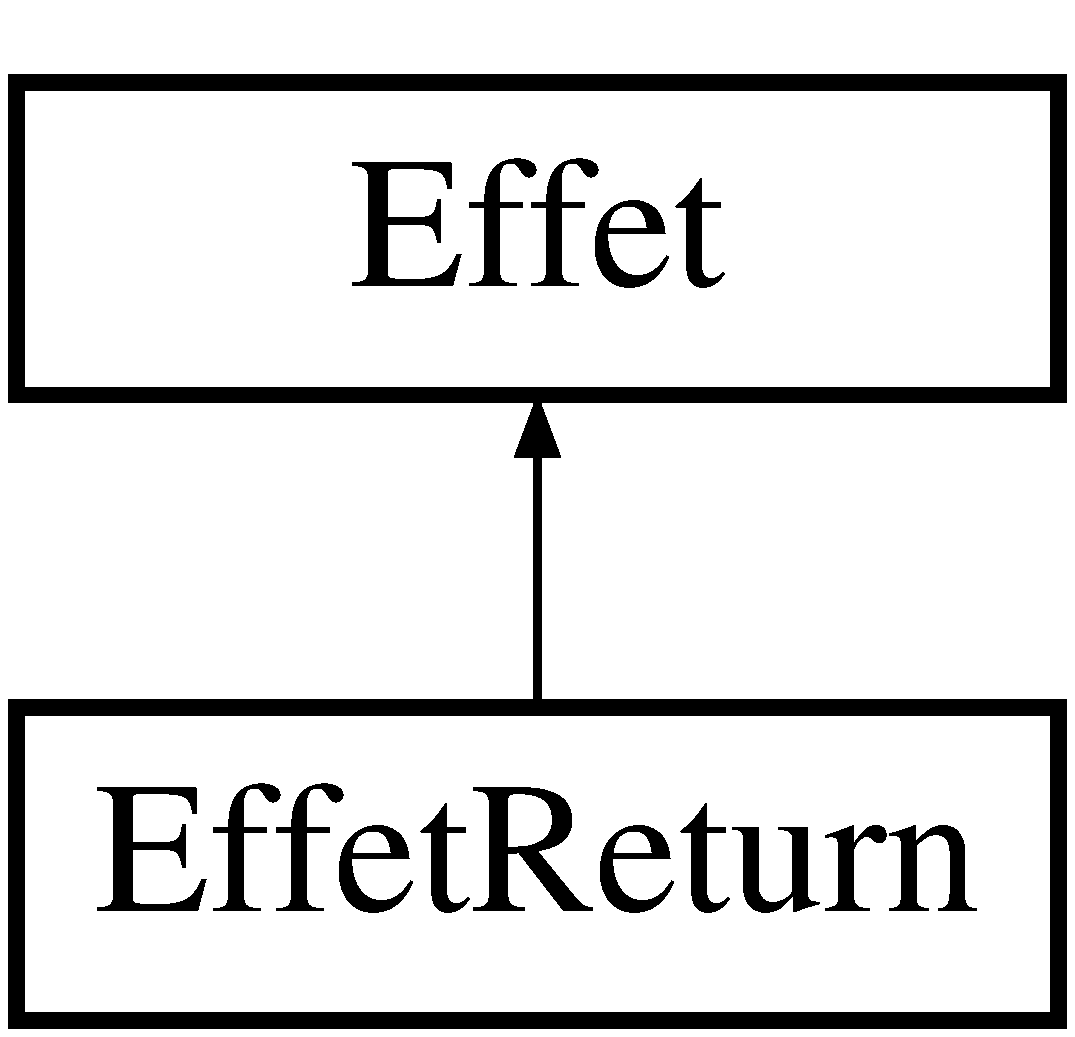
\includegraphics[height=2.000000cm]{class_effet_return}
\end{center}
\end{figure}
\subsection*{Fonctions membres publiques}
\begin{DoxyCompactItemize}
\item 
\hyperlink{class_effet_return_aef927783a08fd85b388a5a614629d2cc}{Effet\-Return} ()
\item 
void \hyperlink{class_effet_return_a9bd08ea82f466e0a0181a83cd1922a52}{action\-Effet} (\hyperlink{class_jeu}{Jeu} $\ast$jeu, int x)
\begin{DoxyCompactList}\small\item\em applique l'effet \end{DoxyCompactList}\item 
void \hyperlink{class_effet_return_aeb7b436619ff6654961fd421c1886be8}{afficher} ()
\begin{DoxyCompactList}\small\item\em affiche le nom de l'effet et ce qu'il fait \end{DoxyCompactList}\item 
std\-::string \hyperlink{class_effet_return_ad8ac1f6ec29d8472a06d0d4d22e5ad8d}{get\-Nom} ()
\begin{DoxyCompactList}\small\item\em va chercher le nom de l'effet \end{DoxyCompactList}\end{DoxyCompactItemize}


\subsection{Documentation des constructeurs et destructeur}
\hypertarget{class_effet_return_aef927783a08fd85b388a5a614629d2cc}{\index{Effet\-Return@{Effet\-Return}!Effet\-Return@{Effet\-Return}}
\index{Effet\-Return@{Effet\-Return}!EffetReturn@{Effet\-Return}}
\subsubsection[{Effet\-Return}]{\setlength{\rightskip}{0pt plus 5cm}Effet\-Return\-::\-Effet\-Return (
\begin{DoxyParamCaption}
{}
\end{DoxyParamCaption}
)\hspace{0.3cm}{\ttfamily [inline]}}}\label{class_effet_return_aef927783a08fd85b388a5a614629d2cc}


\subsection{Documentation des fonctions membres}
\hypertarget{class_effet_return_a9bd08ea82f466e0a0181a83cd1922a52}{\index{Effet\-Return@{Effet\-Return}!action\-Effet@{action\-Effet}}
\index{action\-Effet@{action\-Effet}!EffetReturn@{Effet\-Return}}
\subsubsection[{action\-Effet}]{\setlength{\rightskip}{0pt plus 5cm}void Effet\-Return\-::action\-Effet (
\begin{DoxyParamCaption}
\item[{{\bf Jeu} $\ast$}]{jeu, }
\item[{int}]{x}
\end{DoxyParamCaption}
)\hspace{0.3cm}{\ttfamily [virtual]}}}\label{class_effet_return_a9bd08ea82f466e0a0181a83cd1922a52}


applique l'effet 


\begin{DoxyParams}{Paramètres}
{\em \hyperlink{class_jeu}{Jeu}} & $\ast$jeu \-: le jeu \\
\hline
{\em int} & x \-: le joueur qui joue l'effet \\
\hline
\end{DoxyParams}


Réimplémentée à partir de \hyperlink{class_effet_a57adb1db82d03cda90600f93cc8b5197}{Effet}.

\hypertarget{class_effet_return_aeb7b436619ff6654961fd421c1886be8}{\index{Effet\-Return@{Effet\-Return}!afficher@{afficher}}
\index{afficher@{afficher}!EffetReturn@{Effet\-Return}}
\subsubsection[{afficher}]{\setlength{\rightskip}{0pt plus 5cm}void Effet\-Return\-::afficher (
\begin{DoxyParamCaption}
{}
\end{DoxyParamCaption}
)\hspace{0.3cm}{\ttfamily [virtual]}}}\label{class_effet_return_aeb7b436619ff6654961fd421c1886be8}


affiche le nom de l'effet et ce qu'il fait 



Implémente \hyperlink{class_effet_a1bc485c64cfa136e279d5c9183b3e41d}{Effet}.

\hypertarget{class_effet_return_ad8ac1f6ec29d8472a06d0d4d22e5ad8d}{\index{Effet\-Return@{Effet\-Return}!get\-Nom@{get\-Nom}}
\index{get\-Nom@{get\-Nom}!EffetReturn@{Effet\-Return}}
\subsubsection[{get\-Nom}]{\setlength{\rightskip}{0pt plus 5cm}std\-::string Effet\-Return\-::get\-Nom (
\begin{DoxyParamCaption}
{}
\end{DoxyParamCaption}
)\hspace{0.3cm}{\ttfamily [virtual]}}}\label{class_effet_return_ad8ac1f6ec29d8472a06d0d4d22e5ad8d}


va chercher le nom de l'effet 

\begin{DoxyReturn}{Renvoie}
\-: une string qui corespond au nom de l'effet' 
\end{DoxyReturn}


Implémente \hyperlink{class_effet_a1d3b1a8092df2624399c80d24a21cc88}{Effet}.



La documentation de cette classe a été générée à partir du fichier suivant \-:\begin{DoxyCompactItemize}
\item 
/home/figiel-\/paul/\-Bureau/\-Projet\-Poo/\-Projet\-P\-O\-O-\/\-A\-R\-A\-Y\-A-\/\-F\-I\-G\-I\-E\-L/include/\hyperlink{_effet_return_8hpp}{Effet\-Return.\-hpp}\end{DoxyCompactItemize}

\hypertarget{class_effet_the_answer}{\section{Référence de la classe Effet\-The\-Answer}
\label{class_effet_the_answer}\index{Effet\-The\-Answer@{Effet\-The\-Answer}}
}


{\ttfamily \#include $<$Effet\-The\-Answer.\-hpp$>$}

Graphe d'héritage de Effet\-The\-Answer\-:\begin{figure}[H]
\begin{center}
\leavevmode
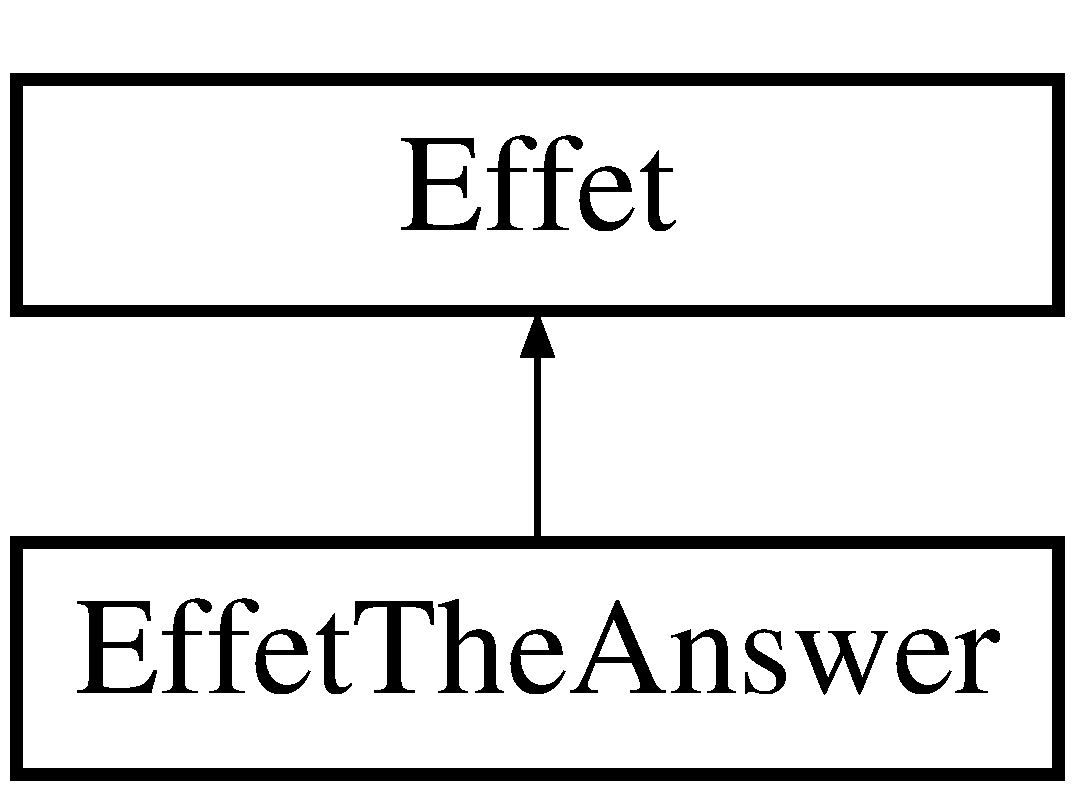
\includegraphics[height=2.000000cm]{class_effet_the_answer}
\end{center}
\end{figure}
\subsection*{Fonctions membres publiques}
\begin{DoxyCompactItemize}
\item 
\hyperlink{class_effet_the_answer_acf8e724a72d1bfc3c5dfe8e2467eff4b}{Effet\-The\-Answer} ()
\item 
void \hyperlink{class_effet_the_answer_a3e8f2cad127fdf393f1421eb04a6ebe8}{action\-Effet} (\hyperlink{class_jeu}{Jeu} $\ast$jeu, int x)
\begin{DoxyCompactList}\small\item\em applique l'effet \end{DoxyCompactList}\item 
void \hyperlink{class_effet_the_answer_a35ba2f942b38ffc60c9c64a763ba77b5}{afficher} ()
\begin{DoxyCompactList}\small\item\em affiche le nom de l'effet et ce qu'il fait \end{DoxyCompactList}\item 
std\-::string \hyperlink{class_effet_the_answer_a4438775df11e19a34226ac8f8b499961}{get\-Nom} ()
\begin{DoxyCompactList}\small\item\em va chercher le nom de l'effet \end{DoxyCompactList}\end{DoxyCompactItemize}


\subsection{Documentation des constructeurs et destructeur}
\hypertarget{class_effet_the_answer_acf8e724a72d1bfc3c5dfe8e2467eff4b}{\index{Effet\-The\-Answer@{Effet\-The\-Answer}!Effet\-The\-Answer@{Effet\-The\-Answer}}
\index{Effet\-The\-Answer@{Effet\-The\-Answer}!EffetTheAnswer@{Effet\-The\-Answer}}
\subsubsection[{Effet\-The\-Answer}]{\setlength{\rightskip}{0pt plus 5cm}Effet\-The\-Answer\-::\-Effet\-The\-Answer (
\begin{DoxyParamCaption}
{}
\end{DoxyParamCaption}
)\hspace{0.3cm}{\ttfamily [inline]}}}\label{class_effet_the_answer_acf8e724a72d1bfc3c5dfe8e2467eff4b}


\subsection{Documentation des fonctions membres}
\hypertarget{class_effet_the_answer_a3e8f2cad127fdf393f1421eb04a6ebe8}{\index{Effet\-The\-Answer@{Effet\-The\-Answer}!action\-Effet@{action\-Effet}}
\index{action\-Effet@{action\-Effet}!EffetTheAnswer@{Effet\-The\-Answer}}
\subsubsection[{action\-Effet}]{\setlength{\rightskip}{0pt plus 5cm}void Effet\-The\-Answer\-::action\-Effet (
\begin{DoxyParamCaption}
\item[{{\bf Jeu} $\ast$}]{jeu, }
\item[{int}]{x}
\end{DoxyParamCaption}
)\hspace{0.3cm}{\ttfamily [virtual]}}}\label{class_effet_the_answer_a3e8f2cad127fdf393f1421eb04a6ebe8}


applique l'effet 


\begin{DoxyParams}{Paramètres}
{\em \hyperlink{class_jeu}{Jeu}} & $\ast$jeu \-: le jeu \\
\hline
{\em int} & x \-: le joueur qui joue l'effet \\
\hline
\end{DoxyParams}


Réimplémentée à partir de \hyperlink{class_effet_a57adb1db82d03cda90600f93cc8b5197}{Effet}.

\hypertarget{class_effet_the_answer_a35ba2f942b38ffc60c9c64a763ba77b5}{\index{Effet\-The\-Answer@{Effet\-The\-Answer}!afficher@{afficher}}
\index{afficher@{afficher}!EffetTheAnswer@{Effet\-The\-Answer}}
\subsubsection[{afficher}]{\setlength{\rightskip}{0pt plus 5cm}void Effet\-The\-Answer\-::afficher (
\begin{DoxyParamCaption}
{}
\end{DoxyParamCaption}
)\hspace{0.3cm}{\ttfamily [virtual]}}}\label{class_effet_the_answer_a35ba2f942b38ffc60c9c64a763ba77b5}


affiche le nom de l'effet et ce qu'il fait 



Implémente \hyperlink{class_effet_a1bc485c64cfa136e279d5c9183b3e41d}{Effet}.

\hypertarget{class_effet_the_answer_a4438775df11e19a34226ac8f8b499961}{\index{Effet\-The\-Answer@{Effet\-The\-Answer}!get\-Nom@{get\-Nom}}
\index{get\-Nom@{get\-Nom}!EffetTheAnswer@{Effet\-The\-Answer}}
\subsubsection[{get\-Nom}]{\setlength{\rightskip}{0pt plus 5cm}std\-::string Effet\-The\-Answer\-::get\-Nom (
\begin{DoxyParamCaption}
{}
\end{DoxyParamCaption}
)\hspace{0.3cm}{\ttfamily [virtual]}}}\label{class_effet_the_answer_a4438775df11e19a34226ac8f8b499961}


va chercher le nom de l'effet 

\begin{DoxyReturn}{Renvoie}
\-: une string qui corespond au nom de l'effet' 
\end{DoxyReturn}


Implémente \hyperlink{class_effet_a1d3b1a8092df2624399c80d24a21cc88}{Effet}.



La documentation de cette classe a été générée à partir du fichier suivant \-:\begin{DoxyCompactItemize}
\item 
/home/figiel-\/paul/\-Bureau/\-Projet\-Poo/\-Projet\-P\-O\-O-\/\-A\-R\-A\-Y\-A-\/\-F\-I\-G\-I\-E\-L/include/\hyperlink{_effet_the_answer_8hpp}{Effet\-The\-Answer.\-hpp}\end{DoxyCompactItemize}

\hypertarget{class_effet_yolo}{\section{Référence de la classe Effet\-Yolo}
\label{class_effet_yolo}\index{Effet\-Yolo@{Effet\-Yolo}}
}


{\ttfamily \#include $<$Effet\-Yolo.\-hpp$>$}

Graphe d'héritage de Effet\-Yolo\-:\begin{figure}[H]
\begin{center}
\leavevmode
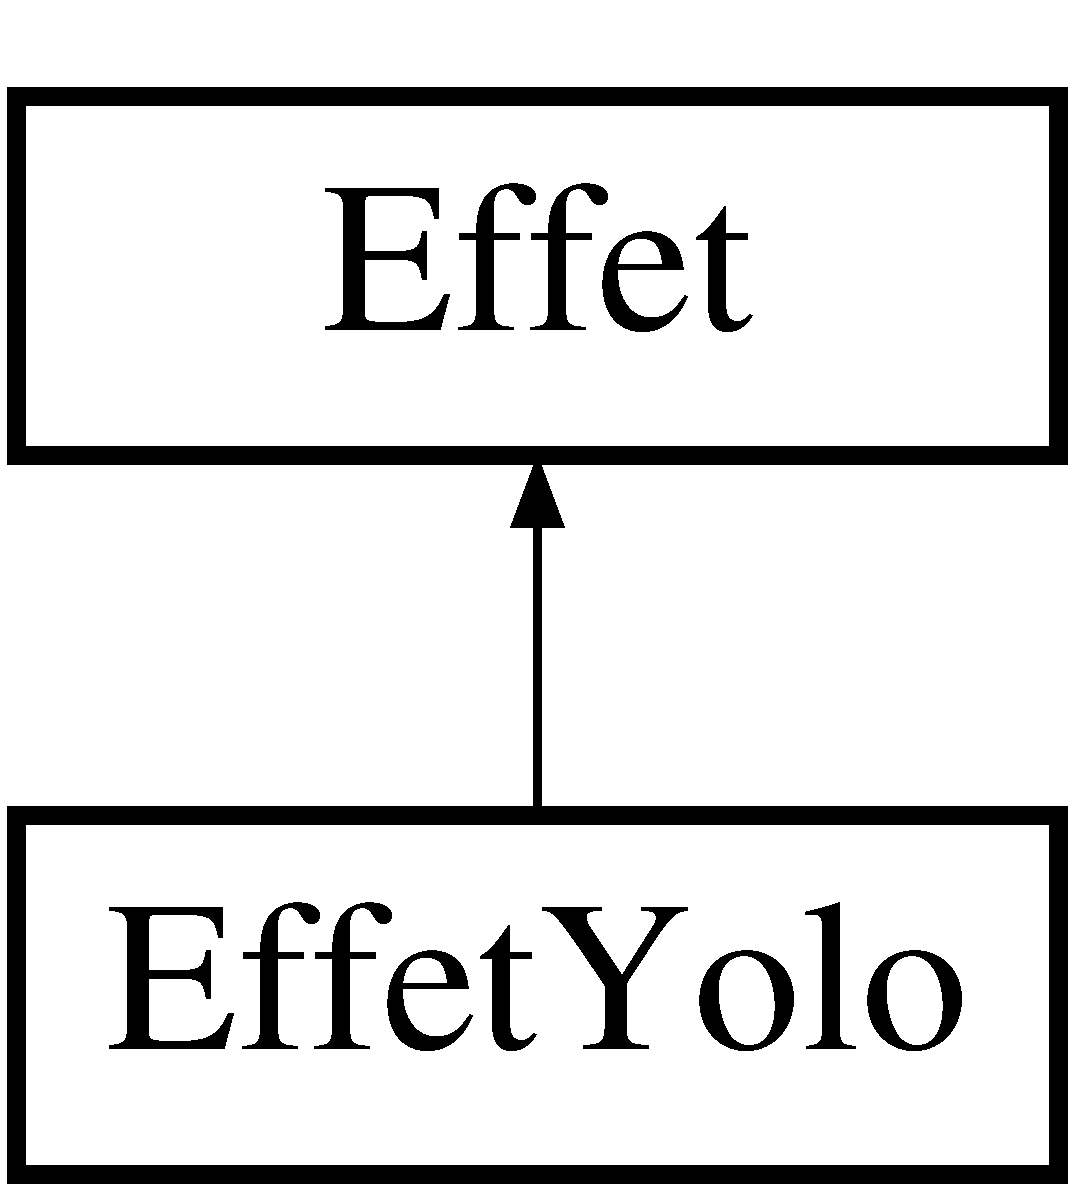
\includegraphics[height=2.000000cm]{class_effet_yolo}
\end{center}
\end{figure}
\subsection*{Fonctions membres publiques}
\begin{DoxyCompactItemize}
\item 
\hyperlink{class_effet_yolo_aaccbf7b9926258bbd683dee0cb930d76}{Effet\-Yolo} ()
\item 
void \hyperlink{class_effet_yolo_abb0ba5ceef4b948c833519557c850cf3}{action\-Effet} (\hyperlink{class_jeu}{Jeu} $\ast$jeu, int x)
\begin{DoxyCompactList}\small\item\em applique l'effet \end{DoxyCompactList}\item 
void \hyperlink{class_effet_yolo_afd45910743596b404709e5da05a507bb}{afficher} ()
\begin{DoxyCompactList}\small\item\em affiche le nom de l'effet et ce qu'il fait \end{DoxyCompactList}\item 
std\-::string \hyperlink{class_effet_yolo_a1118497023e66bc661aca8ba4189f036}{get\-Nom} ()
\begin{DoxyCompactList}\small\item\em va chercher le nom de l'effet \end{DoxyCompactList}\end{DoxyCompactItemize}


\subsection{Documentation des constructeurs et destructeur}
\hypertarget{class_effet_yolo_aaccbf7b9926258bbd683dee0cb930d76}{\index{Effet\-Yolo@{Effet\-Yolo}!Effet\-Yolo@{Effet\-Yolo}}
\index{Effet\-Yolo@{Effet\-Yolo}!EffetYolo@{Effet\-Yolo}}
\subsubsection[{Effet\-Yolo}]{\setlength{\rightskip}{0pt plus 5cm}Effet\-Yolo\-::\-Effet\-Yolo (
\begin{DoxyParamCaption}
{}
\end{DoxyParamCaption}
)\hspace{0.3cm}{\ttfamily [inline]}}}\label{class_effet_yolo_aaccbf7b9926258bbd683dee0cb930d76}


\subsection{Documentation des fonctions membres}
\hypertarget{class_effet_yolo_abb0ba5ceef4b948c833519557c850cf3}{\index{Effet\-Yolo@{Effet\-Yolo}!action\-Effet@{action\-Effet}}
\index{action\-Effet@{action\-Effet}!EffetYolo@{Effet\-Yolo}}
\subsubsection[{action\-Effet}]{\setlength{\rightskip}{0pt plus 5cm}void Effet\-Yolo\-::action\-Effet (
\begin{DoxyParamCaption}
\item[{{\bf Jeu} $\ast$}]{jeu, }
\item[{int}]{x}
\end{DoxyParamCaption}
)\hspace{0.3cm}{\ttfamily [virtual]}}}\label{class_effet_yolo_abb0ba5ceef4b948c833519557c850cf3}


applique l'effet 


\begin{DoxyParams}{Paramètres}
{\em \hyperlink{class_jeu}{Jeu}} & $\ast$jeu \-: le jeu \\
\hline
{\em int} & x \-: le joueur qui joue l'effet \\
\hline
\end{DoxyParams}


Réimplémentée à partir de \hyperlink{class_effet_a57adb1db82d03cda90600f93cc8b5197}{Effet}.

\hypertarget{class_effet_yolo_afd45910743596b404709e5da05a507bb}{\index{Effet\-Yolo@{Effet\-Yolo}!afficher@{afficher}}
\index{afficher@{afficher}!EffetYolo@{Effet\-Yolo}}
\subsubsection[{afficher}]{\setlength{\rightskip}{0pt plus 5cm}void Effet\-Yolo\-::afficher (
\begin{DoxyParamCaption}
{}
\end{DoxyParamCaption}
)\hspace{0.3cm}{\ttfamily [virtual]}}}\label{class_effet_yolo_afd45910743596b404709e5da05a507bb}


affiche le nom de l'effet et ce qu'il fait 



Implémente \hyperlink{class_effet_a1bc485c64cfa136e279d5c9183b3e41d}{Effet}.

\hypertarget{class_effet_yolo_a1118497023e66bc661aca8ba4189f036}{\index{Effet\-Yolo@{Effet\-Yolo}!get\-Nom@{get\-Nom}}
\index{get\-Nom@{get\-Nom}!EffetYolo@{Effet\-Yolo}}
\subsubsection[{get\-Nom}]{\setlength{\rightskip}{0pt plus 5cm}std\-::string Effet\-Yolo\-::get\-Nom (
\begin{DoxyParamCaption}
{}
\end{DoxyParamCaption}
)\hspace{0.3cm}{\ttfamily [virtual]}}}\label{class_effet_yolo_a1118497023e66bc661aca8ba4189f036}


va chercher le nom de l'effet 

\begin{DoxyReturn}{Renvoie}
\-: une string qui corespond au nom de l'effet' 
\end{DoxyReturn}


Implémente \hyperlink{class_effet_a1d3b1a8092df2624399c80d24a21cc88}{Effet}.



La documentation de cette classe a été générée à partir du fichier suivant \-:\begin{DoxyCompactItemize}
\item 
/home/figiel-\/paul/\-Bureau/\-Projet\-Poo/\-Projet\-P\-O\-O-\/\-A\-R\-A\-Y\-A-\/\-F\-I\-G\-I\-E\-L/include/\hyperlink{_effet_yolo_8hpp}{Effet\-Yolo.\-hpp}\end{DoxyCompactItemize}

\hypertarget{class_etat}{\section{Référence de la classe Etat}
\label{class_etat}\index{Etat@{Etat}}
}


{\ttfamily \#include $<$Etat.\-hpp$>$}

Graphe d'héritage de Etat\-:\begin{figure}[H]
\begin{center}
\leavevmode
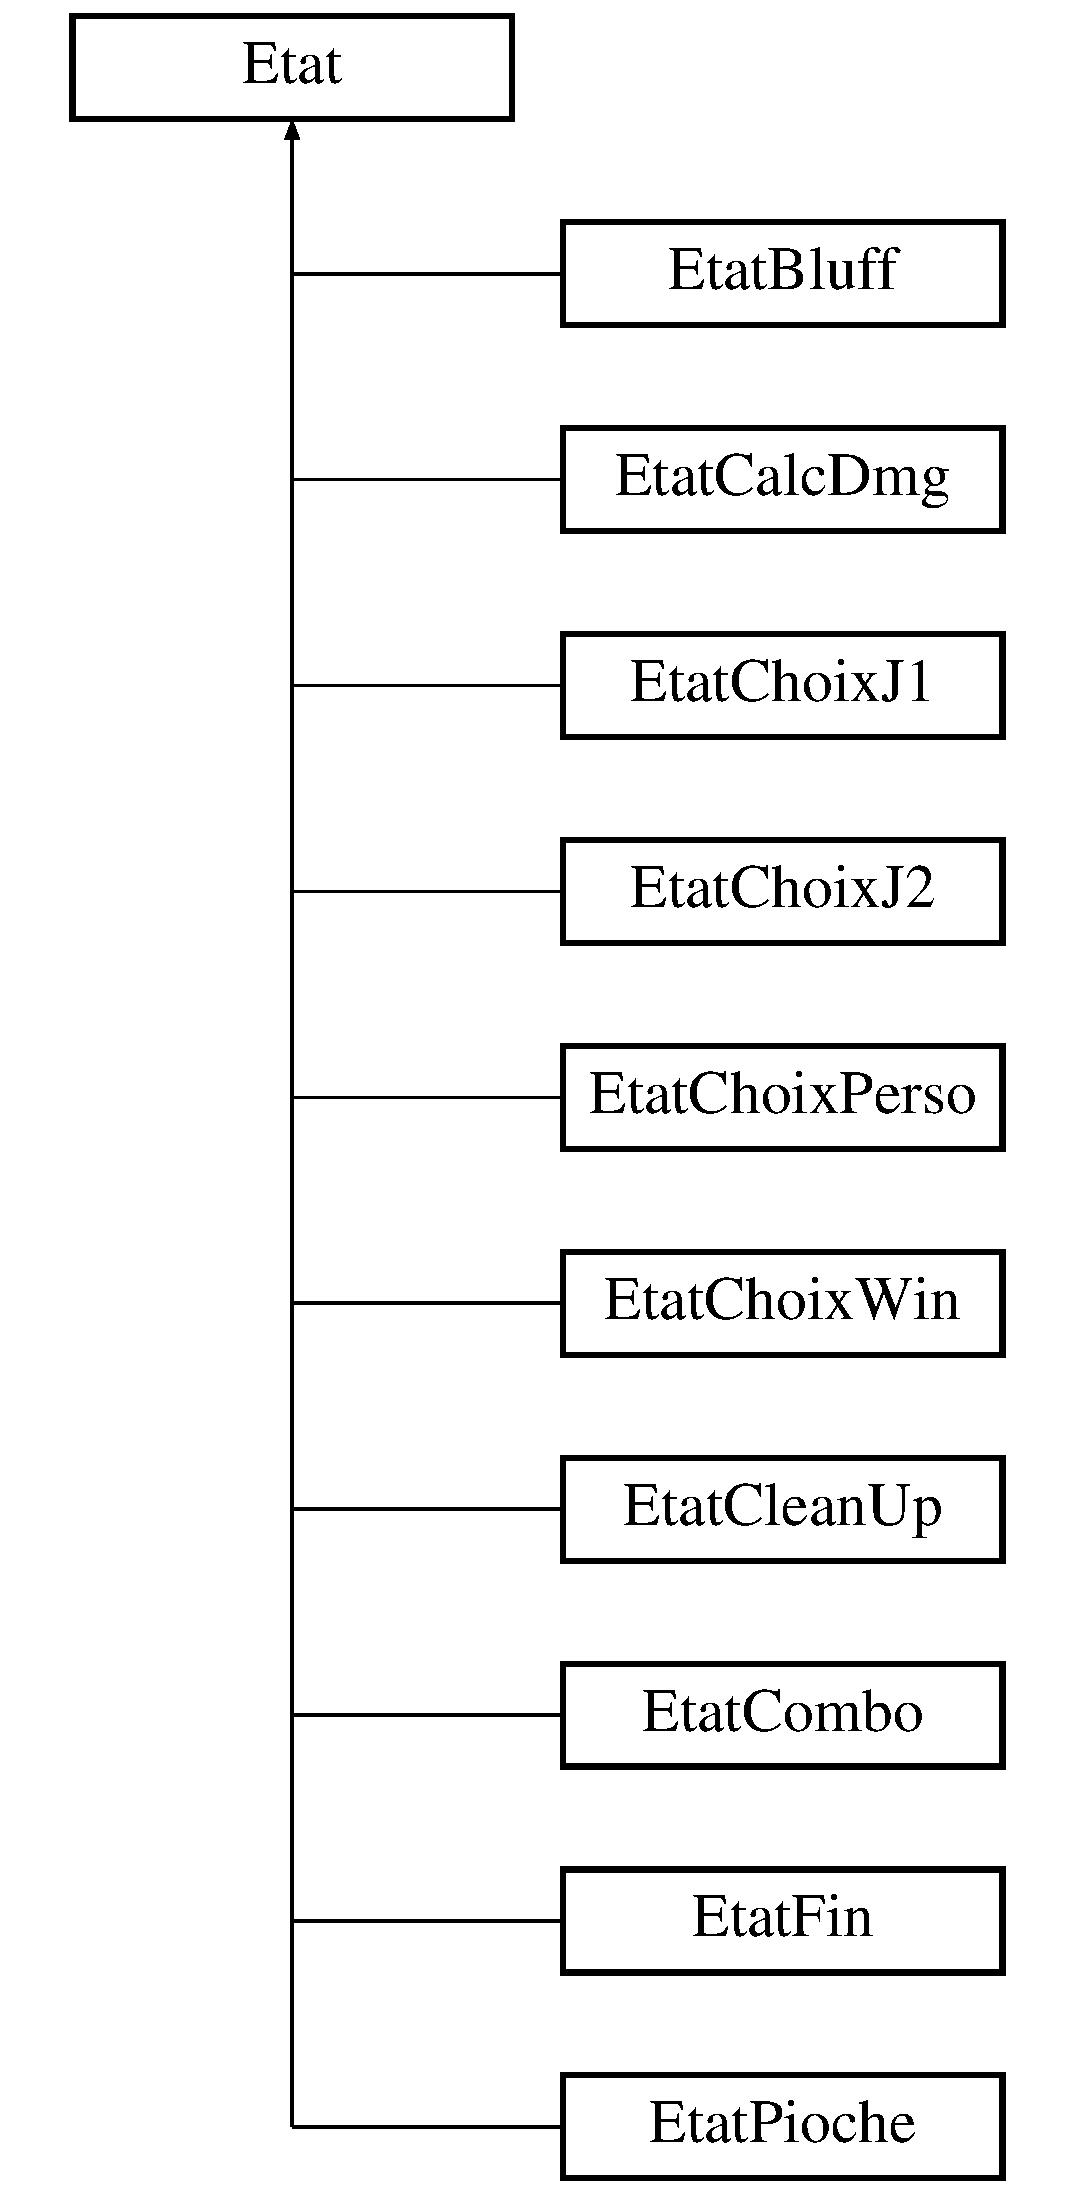
\includegraphics[height=11.000000cm]{class_etat}
\end{center}
\end{figure}
\subsection*{Fonctions membres publiques}
\begin{DoxyCompactItemize}
\item 
virtual void \hyperlink{class_etat_aaf949c7b45217b76ff68414e61ef0d2a}{verification} ()=0
\begin{DoxyCompactList}\small\item\em procéde au diverse vérification (varie selon l'état). \end{DoxyCompactList}\item 
virtual void \hyperlink{class_etat_afd99ba60265bc0a82029d5fa2368acfa}{Info\-Carte} ()=0
\begin{DoxyCompactList}\small\item\em affiche l'info d'une carte (varie selon l'état). \end{DoxyCompactList}\item 
virtual void \hyperlink{class_etat_a3d2fe662ffd20147763a25c4e06b56e9}{retourner\-Carte} ()=0
\begin{DoxyCompactList}\small\item\em retourne la dérnière carte jouer dans la main de son propriétaire (varie selon l'état). \end{DoxyCompactList}\item 
virtual void \hyperlink{class_etat_aaeffe08c27b2b64560726f5df95e6f3a}{jouer\-Carte} ()=0
\begin{DoxyCompactList}\small\item\em joue une carte (varie selon l'état). \end{DoxyCompactList}\item 
virtual void \hyperlink{class_etat_a65c2e505cda8cac2989b3a0c17a70278}{confirmation} ()=0
\begin{DoxyCompactList}\small\item\em confirme l'action (varie selon l'état). \end{DoxyCompactList}\item 
virtual void \hyperlink{class_etat_ac47332db984da58192bbb1c45f1702a8}{annuler\-Action} ()=0
\begin{DoxyCompactList}\small\item\em annule l'action (varie selon l'état). \end{DoxyCompactList}\end{DoxyCompactItemize}


\subsection{Documentation des fonctions membres}
\hypertarget{class_etat_ac47332db984da58192bbb1c45f1702a8}{\index{Etat@{Etat}!annuler\-Action@{annuler\-Action}}
\index{annuler\-Action@{annuler\-Action}!Etat@{Etat}}
\subsubsection[{annuler\-Action}]{\setlength{\rightskip}{0pt plus 5cm}virtual void Etat\-::annuler\-Action (
\begin{DoxyParamCaption}
{}
\end{DoxyParamCaption}
)\hspace{0.3cm}{\ttfamily [pure virtual]}}}\label{class_etat_ac47332db984da58192bbb1c45f1702a8}


annule l'action (varie selon l'état). 



Implémenté dans \hyperlink{class_etat_bluff_ac570a417e0c4d1e766ff29b8f02eac0a}{Etat\-Bluff}, \hyperlink{class_etat_calc_dmg_af9ef4c658d2591d25e03fabaa5d9bca1}{Etat\-Calc\-Dmg}, \hyperlink{class_etat_choix_j2_a076a02ef80e3dded9fb3df17dd23542a}{Etat\-Choix\-J2}, \hyperlink{class_etat_choix_j1_af6a16d04020f3079a6a02e5cae8860ec}{Etat\-Choix\-J1}, \hyperlink{class_etat_clean_up_a7163c116050f238c7bcd43a7e9bae974}{Etat\-Clean\-Up}, \hyperlink{class_etat_pioche_a5c22d5a85ff1d59eb5facecee39e960b}{Etat\-Pioche}, \hyperlink{class_etat_choix_win_ae321052d630a6a679f6347c36f580ea7}{Etat\-Choix\-Win}, \hyperlink{class_etat_combo_a18e6acc9e6e6a9db9a217d9aa044d778}{Etat\-Combo}, \hyperlink{class_etat_fin_aa1ec559bd55dce76286b32b4cb293857}{Etat\-Fin}, et \hyperlink{class_etat_choix_perso_a1a67ae6bf8cf6cd9c79afd84b1961385}{Etat\-Choix\-Perso}.

\hypertarget{class_etat_a65c2e505cda8cac2989b3a0c17a70278}{\index{Etat@{Etat}!confirmation@{confirmation}}
\index{confirmation@{confirmation}!Etat@{Etat}}
\subsubsection[{confirmation}]{\setlength{\rightskip}{0pt plus 5cm}virtual void Etat\-::confirmation (
\begin{DoxyParamCaption}
{}
\end{DoxyParamCaption}
)\hspace{0.3cm}{\ttfamily [pure virtual]}}}\label{class_etat_a65c2e505cda8cac2989b3a0c17a70278}


confirme l'action (varie selon l'état). 



Implémenté dans \hyperlink{class_etat_choix_j2_af09ee4f38957e7fe8232db7dcfccd573}{Etat\-Choix\-J2}, \hyperlink{class_etat_bluff_a7933ee4cc543982cdfe62bfe1a50c765}{Etat\-Bluff}, \hyperlink{class_etat_calc_dmg_a6b33fa83c3897ce65ed53b6b345615c1}{Etat\-Calc\-Dmg}, \hyperlink{class_etat_choix_j1_a7c9397632889bb66bdd5a635ab7ad3cb}{Etat\-Choix\-J1}, \hyperlink{class_etat_clean_up_a4c0dbb8c302a500052eccdc66c6a28b4}{Etat\-Clean\-Up}, \hyperlink{class_etat_pioche_ab3394a63db70d706b48501969edc7880}{Etat\-Pioche}, \hyperlink{class_etat_choix_win_aef8d0abe059050e7a7e3e598c87de992}{Etat\-Choix\-Win}, \hyperlink{class_etat_combo_a26ed3a79035572c4471aab88377470c5}{Etat\-Combo}, \hyperlink{class_etat_fin_a218360ae56a421d500329f53c893822e}{Etat\-Fin}, et \hyperlink{class_etat_choix_perso_a60ea227168029d7741f2919d73b8d2cc}{Etat\-Choix\-Perso}.

\hypertarget{class_etat_afd99ba60265bc0a82029d5fa2368acfa}{\index{Etat@{Etat}!Info\-Carte@{Info\-Carte}}
\index{Info\-Carte@{Info\-Carte}!Etat@{Etat}}
\subsubsection[{Info\-Carte}]{\setlength{\rightskip}{0pt plus 5cm}virtual void Etat\-::\-Info\-Carte (
\begin{DoxyParamCaption}
{}
\end{DoxyParamCaption}
)\hspace{0.3cm}{\ttfamily [pure virtual]}}}\label{class_etat_afd99ba60265bc0a82029d5fa2368acfa}


affiche l'info d'une carte (varie selon l'état). 



Implémenté dans \hyperlink{class_etat_choix_j2_ab0066e2aa95ddfe577d0e9ba4ae5441e}{Etat\-Choix\-J2}, \hyperlink{class_etat_choix_j1_aeb4984f144a61f1a98120dc844364212}{Etat\-Choix\-J1}, \hyperlink{class_etat_bluff_a9a50082e841c2ef7781795d546d77b3e}{Etat\-Bluff}, \hyperlink{class_etat_calc_dmg_a3d68b599faab01efda64cf48a336ec29}{Etat\-Calc\-Dmg}, \hyperlink{class_etat_clean_up_aac0dacd1f4945a971ec72319c979a786}{Etat\-Clean\-Up}, \hyperlink{class_etat_pioche_aa4379e774a3cfa7f3ce7f6668363f04f}{Etat\-Pioche}, \hyperlink{class_etat_choix_win_af5143e3b6e6c80633b48fcbc9fa52be2}{Etat\-Choix\-Win}, \hyperlink{class_etat_combo_a56b4cbe699ca50fc0e6ad4695a744bdf}{Etat\-Combo}, \hyperlink{class_etat_fin_a60377a6cd48de413cb14445f8e9683bb}{Etat\-Fin}, et \hyperlink{class_etat_choix_perso_a10dcb32108b4d457bd58ad45abf6706a}{Etat\-Choix\-Perso}.

\hypertarget{class_etat_aaeffe08c27b2b64560726f5df95e6f3a}{\index{Etat@{Etat}!jouer\-Carte@{jouer\-Carte}}
\index{jouer\-Carte@{jouer\-Carte}!Etat@{Etat}}
\subsubsection[{jouer\-Carte}]{\setlength{\rightskip}{0pt plus 5cm}virtual void Etat\-::jouer\-Carte (
\begin{DoxyParamCaption}
{}
\end{DoxyParamCaption}
)\hspace{0.3cm}{\ttfamily [pure virtual]}}}\label{class_etat_aaeffe08c27b2b64560726f5df95e6f3a}


joue une carte (varie selon l'état). 



Implémenté dans \hyperlink{class_etat_choix_j2_a674ef9e896f33d70cf8937b4591faae9}{Etat\-Choix\-J2}, \hyperlink{class_etat_bluff_a087b8aa9f445736eba04d9811b3ec8e8}{Etat\-Bluff}, \hyperlink{class_etat_calc_dmg_a67193b64493418f62457259688fbe402}{Etat\-Calc\-Dmg}, \hyperlink{class_etat_choix_j1_a5aa86ab5766846edd95a5f82943855a1}{Etat\-Choix\-J1}, \hyperlink{class_etat_clean_up_a3be20ce132ee978e5412ae54f36e4a78}{Etat\-Clean\-Up}, \hyperlink{class_etat_pioche_a951f62c333a41232cb4c09738925e7db}{Etat\-Pioche}, \hyperlink{class_etat_choix_win_a32f02c55bfbf8b580dee3bd95ce1921e}{Etat\-Choix\-Win}, \hyperlink{class_etat_combo_a6d7b6c040664a4c41380aca95f05f42c}{Etat\-Combo}, \hyperlink{class_etat_fin_a8120a04c2f2e3632683a79a6b2fd524a}{Etat\-Fin}, et \hyperlink{class_etat_choix_perso_a31908b4127aeff26b214d470ef22eacb}{Etat\-Choix\-Perso}.

\hypertarget{class_etat_a3d2fe662ffd20147763a25c4e06b56e9}{\index{Etat@{Etat}!retourner\-Carte@{retourner\-Carte}}
\index{retourner\-Carte@{retourner\-Carte}!Etat@{Etat}}
\subsubsection[{retourner\-Carte}]{\setlength{\rightskip}{0pt plus 5cm}virtual void Etat\-::retourner\-Carte (
\begin{DoxyParamCaption}
{}
\end{DoxyParamCaption}
)\hspace{0.3cm}{\ttfamily [pure virtual]}}}\label{class_etat_a3d2fe662ffd20147763a25c4e06b56e9}


retourne la dérnière carte jouer dans la main de son propriétaire (varie selon l'état). 



Implémenté dans \hyperlink{class_etat_choix_j2_a2fe8000154f582684c9a0162bb860b9f}{Etat\-Choix\-J2}, \hyperlink{class_etat_bluff_ad5f658d6e71112d9489927104cc4da4c}{Etat\-Bluff}, \hyperlink{class_etat_choix_j1_a923857828b87f0bde7661e4f7a17efee}{Etat\-Choix\-J1}, \hyperlink{class_etat_calc_dmg_a5b089ca3e4773afc4503106effe36866}{Etat\-Calc\-Dmg}, \hyperlink{class_etat_clean_up_a955f6fb5a4cffdbdca4348b90d59ad78}{Etat\-Clean\-Up}, \hyperlink{class_etat_pioche_ab139c9695f98b2e45df5fdc8f494ea80}{Etat\-Pioche}, \hyperlink{class_etat_choix_win_a583e3a7b7d7e922a74a4609d31c277ee}{Etat\-Choix\-Win}, \hyperlink{class_etat_combo_a79944dfd6e471b633ad99cd2f3b70b02}{Etat\-Combo}, \hyperlink{class_etat_fin_a7772020d9101b4ebac666c498f023215}{Etat\-Fin}, et \hyperlink{class_etat_choix_perso_a5a9e8efb87e8ebb31c0f4db269e938a9}{Etat\-Choix\-Perso}.

\hypertarget{class_etat_aaf949c7b45217b76ff68414e61ef0d2a}{\index{Etat@{Etat}!verification@{verification}}
\index{verification@{verification}!Etat@{Etat}}
\subsubsection[{verification}]{\setlength{\rightskip}{0pt plus 5cm}virtual void Etat\-::verification (
\begin{DoxyParamCaption}
{}
\end{DoxyParamCaption}
)\hspace{0.3cm}{\ttfamily [pure virtual]}}}\label{class_etat_aaf949c7b45217b76ff68414e61ef0d2a}


procéde au diverse vérification (varie selon l'état). 



Implémenté dans \hyperlink{class_etat_choix_j2_a93667fd195d816e8d3e8e26d16a86848}{Etat\-Choix\-J2}, \hyperlink{class_etat_choix_j1_afb7b74d31ac30f1993cd6ae35ff72733}{Etat\-Choix\-J1}, \hyperlink{class_etat_bluff_a87a7f546cb71b52ac869ac41439d49bf}{Etat\-Bluff}, \hyperlink{class_etat_pioche_af429306bdc936b19982b604a686a230d}{Etat\-Pioche}, \hyperlink{class_etat_calc_dmg_abddaaca7a79022a6521e893003240de1}{Etat\-Calc\-Dmg}, \hyperlink{class_etat_clean_up_a58245fa6e240c4c4f20d1a1fca868571}{Etat\-Clean\-Up}, \hyperlink{class_etat_fin_af5b612f37d0d38878b7380c7c44c8373}{Etat\-Fin}, \hyperlink{class_etat_choix_win_ae4b933e5eb219ad05263447db0d970e2}{Etat\-Choix\-Win}, \hyperlink{class_etat_combo_a0a299d7c93ef09787eb0a402708475f0}{Etat\-Combo}, et \hyperlink{class_etat_choix_perso_a18678f06f60115999dd92b8b88dbe7dd}{Etat\-Choix\-Perso}.



La documentation de cette classe a été générée à partir du fichier suivant \-:\begin{DoxyCompactItemize}
\item 
/home/figiel-\/paul/\-Bureau/\-Projet\-Poo/\-Projet\-P\-O\-O-\/\-A\-R\-A\-Y\-A-\/\-F\-I\-G\-I\-E\-L/include/\hyperlink{_etat_8hpp}{Etat.\-hpp}\end{DoxyCompactItemize}

\hypertarget{class_etat_bluff}{\section{Référence de la classe Etat\-Bluff}
\label{class_etat_bluff}\index{Etat\-Bluff@{Etat\-Bluff}}
}


{\ttfamily \#include $<$Etat\-Bluff.\-hpp$>$}

Graphe d'héritage de Etat\-Bluff\-:\begin{figure}[H]
\begin{center}
\leavevmode
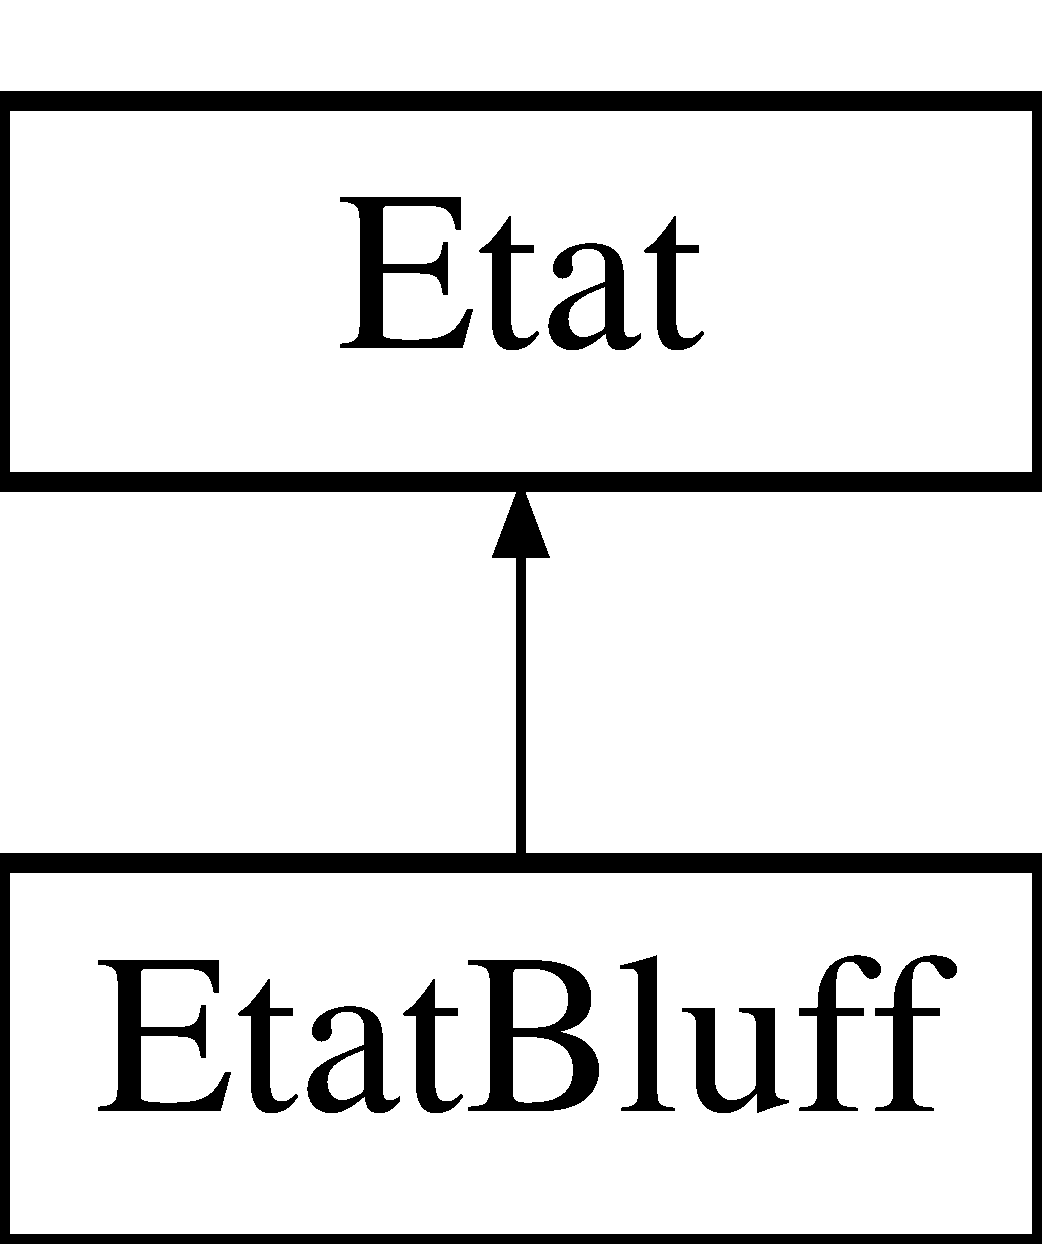
\includegraphics[height=2.000000cm]{class_etat_bluff}
\end{center}
\end{figure}
\subsection*{Fonctions membres publiques}
\begin{DoxyCompactItemize}
\item 
\hyperlink{class_etat_bluff_adf5d424eb972450d3a78cc8974a6be44}{Etat\-Bluff} (\hyperlink{class_jeu}{Jeu} $\ast$jeu)
\begin{DoxyCompactList}\small\item\em Constructeur. \end{DoxyCompactList}\item 
void \hyperlink{class_etat_bluff_a87a7f546cb71b52ac869ac41439d49bf}{verification} ()
\begin{DoxyCompactList}\small\item\em \hyperlink{class_etat_bluff}{Etat\-Bluff} \-: vérifie l'effet de la carte jouer en bluff et si c'est un joker. \end{DoxyCompactList}\item 
void \hyperlink{class_etat_bluff_a9a50082e841c2ef7781795d546d77b3e}{Info\-Carte} ()
\begin{DoxyCompactList}\small\item\em \hyperlink{class_etat_bluff}{Etat\-Bluff} \-: demande un numéro et affiche les infos de la carte corespondante dans la main du joueur qui bluff. \end{DoxyCompactList}\item 
void \hyperlink{class_etat_bluff_ad5f658d6e71112d9489927104cc4da4c}{retourner\-Carte} ()
\begin{DoxyCompactList}\small\item\em \hyperlink{class_etat_bluff}{Etat\-Bluff} \-: demande un numéro et retourne la carte corespondante de la main du joueur qui bluff. \end{DoxyCompactList}\item 
void \hyperlink{class_etat_bluff_a087b8aa9f445736eba04d9811b3ec8e8}{jouer\-Carte} ()
\begin{DoxyCompactList}\small\item\em \hyperlink{class_etat_bluff}{Etat\-Bluff} \-: demande un numéro et joue la carte corespondante de la main du joueur qui bluff (demande confirmation). \end{DoxyCompactList}\item 
void \hyperlink{class_etat_bluff_a7933ee4cc543982cdfe62bfe1a50c765}{confirmation} ()
\begin{DoxyCompactList}\small\item\em \hyperlink{class_etat_bluff}{Etat\-Bluff} \-: si le joueur décide de confirmer qu'il veut jouer la carte qu'il vient de posé apelle vérification et passe au prochain état. \end{DoxyCompactList}\item 
void \hyperlink{class_etat_bluff_ac570a417e0c4d1e766ff29b8f02eac0a}{annuler\-Action} ()
\begin{DoxyCompactList}\small\item\em \hyperlink{class_etat_bluff}{Etat\-Bluff} \-: si le joueur décide qu'il ne veut pas jouer la carte qu'il vient de posé la renvoie dans sa main. \end{DoxyCompactList}\end{DoxyCompactItemize}


\subsection{Documentation des constructeurs et destructeur}
\hypertarget{class_etat_bluff_adf5d424eb972450d3a78cc8974a6be44}{\index{Etat\-Bluff@{Etat\-Bluff}!Etat\-Bluff@{Etat\-Bluff}}
\index{Etat\-Bluff@{Etat\-Bluff}!EtatBluff@{Etat\-Bluff}}
\subsubsection[{Etat\-Bluff}]{\setlength{\rightskip}{0pt plus 5cm}Etat\-Bluff\-::\-Etat\-Bluff (
\begin{DoxyParamCaption}
\item[{{\bf Jeu} $\ast$}]{jeu}
\end{DoxyParamCaption}
)\hspace{0.3cm}{\ttfamily [inline]}}}\label{class_etat_bluff_adf5d424eb972450d3a78cc8974a6be44}


Constructeur. 

Constructeur de la classe \hyperlink{class_etat_bluff}{Etat\-Bluff}


\begin{DoxyParams}{Paramètres}
{\em jeu} & \-: pointeur vers le jeu \\
\hline
\end{DoxyParams}


\subsection{Documentation des fonctions membres}
\hypertarget{class_etat_bluff_ac570a417e0c4d1e766ff29b8f02eac0a}{\index{Etat\-Bluff@{Etat\-Bluff}!annuler\-Action@{annuler\-Action}}
\index{annuler\-Action@{annuler\-Action}!EtatBluff@{Etat\-Bluff}}
\subsubsection[{annuler\-Action}]{\setlength{\rightskip}{0pt plus 5cm}void Etat\-Bluff\-::annuler\-Action (
\begin{DoxyParamCaption}
{}
\end{DoxyParamCaption}
)\hspace{0.3cm}{\ttfamily [virtual]}}}\label{class_etat_bluff_ac570a417e0c4d1e766ff29b8f02eac0a}


\hyperlink{class_etat_bluff}{Etat\-Bluff} \-: si le joueur décide qu'il ne veut pas jouer la carte qu'il vient de posé la renvoie dans sa main. 



Implémente \hyperlink{class_etat_ac47332db984da58192bbb1c45f1702a8}{Etat}.

\hypertarget{class_etat_bluff_a7933ee4cc543982cdfe62bfe1a50c765}{\index{Etat\-Bluff@{Etat\-Bluff}!confirmation@{confirmation}}
\index{confirmation@{confirmation}!EtatBluff@{Etat\-Bluff}}
\subsubsection[{confirmation}]{\setlength{\rightskip}{0pt plus 5cm}void Etat\-Bluff\-::confirmation (
\begin{DoxyParamCaption}
{}
\end{DoxyParamCaption}
)\hspace{0.3cm}{\ttfamily [virtual]}}}\label{class_etat_bluff_a7933ee4cc543982cdfe62bfe1a50c765}


\hyperlink{class_etat_bluff}{Etat\-Bluff} \-: si le joueur décide de confirmer qu'il veut jouer la carte qu'il vient de posé apelle vérification et passe au prochain état. 



Implémente \hyperlink{class_etat_a65c2e505cda8cac2989b3a0c17a70278}{Etat}.

\hypertarget{class_etat_bluff_a9a50082e841c2ef7781795d546d77b3e}{\index{Etat\-Bluff@{Etat\-Bluff}!Info\-Carte@{Info\-Carte}}
\index{Info\-Carte@{Info\-Carte}!EtatBluff@{Etat\-Bluff}}
\subsubsection[{Info\-Carte}]{\setlength{\rightskip}{0pt plus 5cm}void Etat\-Bluff\-::\-Info\-Carte (
\begin{DoxyParamCaption}
{}
\end{DoxyParamCaption}
)\hspace{0.3cm}{\ttfamily [virtual]}}}\label{class_etat_bluff_a9a50082e841c2ef7781795d546d77b3e}


\hyperlink{class_etat_bluff}{Etat\-Bluff} \-: demande un numéro et affiche les infos de la carte corespondante dans la main du joueur qui bluff. 



Implémente \hyperlink{class_etat_afd99ba60265bc0a82029d5fa2368acfa}{Etat}.

\hypertarget{class_etat_bluff_a087b8aa9f445736eba04d9811b3ec8e8}{\index{Etat\-Bluff@{Etat\-Bluff}!jouer\-Carte@{jouer\-Carte}}
\index{jouer\-Carte@{jouer\-Carte}!EtatBluff@{Etat\-Bluff}}
\subsubsection[{jouer\-Carte}]{\setlength{\rightskip}{0pt plus 5cm}void Etat\-Bluff\-::jouer\-Carte (
\begin{DoxyParamCaption}
{}
\end{DoxyParamCaption}
)\hspace{0.3cm}{\ttfamily [virtual]}}}\label{class_etat_bluff_a087b8aa9f445736eba04d9811b3ec8e8}


\hyperlink{class_etat_bluff}{Etat\-Bluff} \-: demande un numéro et joue la carte corespondante de la main du joueur qui bluff (demande confirmation). 



Implémente \hyperlink{class_etat_aaeffe08c27b2b64560726f5df95e6f3a}{Etat}.

\hypertarget{class_etat_bluff_ad5f658d6e71112d9489927104cc4da4c}{\index{Etat\-Bluff@{Etat\-Bluff}!retourner\-Carte@{retourner\-Carte}}
\index{retourner\-Carte@{retourner\-Carte}!EtatBluff@{Etat\-Bluff}}
\subsubsection[{retourner\-Carte}]{\setlength{\rightskip}{0pt plus 5cm}void Etat\-Bluff\-::retourner\-Carte (
\begin{DoxyParamCaption}
{}
\end{DoxyParamCaption}
)\hspace{0.3cm}{\ttfamily [virtual]}}}\label{class_etat_bluff_ad5f658d6e71112d9489927104cc4da4c}


\hyperlink{class_etat_bluff}{Etat\-Bluff} \-: demande un numéro et retourne la carte corespondante de la main du joueur qui bluff. 



Implémente \hyperlink{class_etat_a3d2fe662ffd20147763a25c4e06b56e9}{Etat}.

\hypertarget{class_etat_bluff_a87a7f546cb71b52ac869ac41439d49bf}{\index{Etat\-Bluff@{Etat\-Bluff}!verification@{verification}}
\index{verification@{verification}!EtatBluff@{Etat\-Bluff}}
\subsubsection[{verification}]{\setlength{\rightskip}{0pt plus 5cm}void Etat\-Bluff\-::verification (
\begin{DoxyParamCaption}
{}
\end{DoxyParamCaption}
)\hspace{0.3cm}{\ttfamily [virtual]}}}\label{class_etat_bluff_a87a7f546cb71b52ac869ac41439d49bf}


\hyperlink{class_etat_bluff}{Etat\-Bluff} \-: vérifie l'effet de la carte jouer en bluff et si c'est un joker. 



Implémente \hyperlink{class_etat_aaf949c7b45217b76ff68414e61ef0d2a}{Etat}.



La documentation de cette classe a été générée à partir du fichier suivant \-:\begin{DoxyCompactItemize}
\item 
/home/figiel-\/paul/\-Bureau/\-Projet\-Poo/\-Projet\-P\-O\-O-\/\-A\-R\-A\-Y\-A-\/\-F\-I\-G\-I\-E\-L/include/\hyperlink{_etat_bluff_8hpp}{Etat\-Bluff.\-hpp}\end{DoxyCompactItemize}

\hypertarget{class_etat_calc_dmg}{\section{Référence de la classe Etat\-Calc\-Dmg}
\label{class_etat_calc_dmg}\index{Etat\-Calc\-Dmg@{Etat\-Calc\-Dmg}}
}


{\ttfamily \#include $<$Etat\-Calc\-Dmg.\-hpp$>$}

Graphe d'héritage de Etat\-Calc\-Dmg\-:\begin{figure}[H]
\begin{center}
\leavevmode
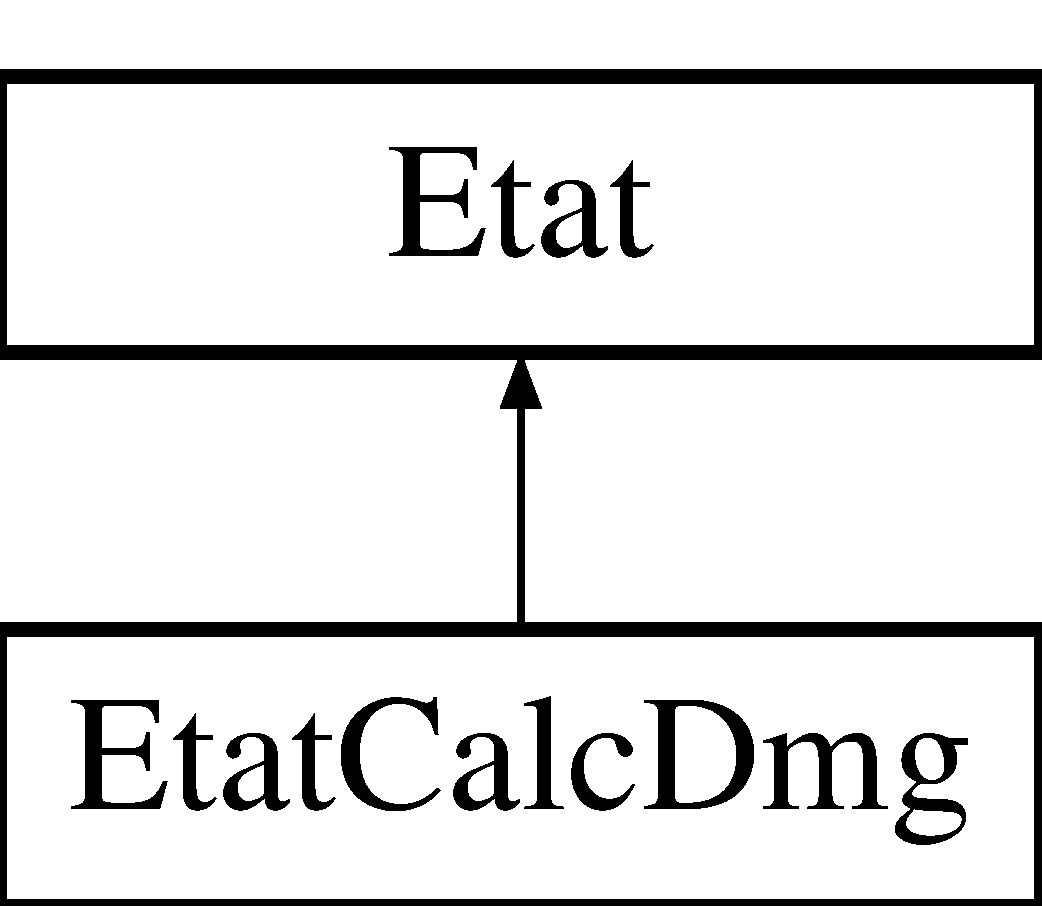
\includegraphics[height=2.000000cm]{class_etat_calc_dmg}
\end{center}
\end{figure}
\subsection*{Fonctions membres publiques}
\begin{DoxyCompactItemize}
\item 
\hyperlink{class_etat_calc_dmg_ab5d3054fd32a3a29c6c234b577cbf8d4}{Etat\-Calc\-Dmg} (\hyperlink{class_jeu}{Jeu} $\ast$jeu)
\begin{DoxyCompactList}\small\item\em Constructeur. \end{DoxyCompactList}\item 
void \hyperlink{class_etat_calc_dmg_abddaaca7a79022a6521e893003240de1}{verification} ()
\begin{DoxyCompactList}\small\item\em \hyperlink{class_etat_calc_dmg}{Etat\-Calc\-Dmg} \-: procédè à toutes les vérification nécessaire et inflige les dégât qu'il faut au deux joueur et passe à l'état clean up. \end{DoxyCompactList}\item 
void \hyperlink{class_etat_calc_dmg_a3d68b599faab01efda64cf48a336ec29}{Info\-Carte} ()
\begin{DoxyCompactList}\small\item\em \hyperlink{class_etat_calc_dmg}{Etat\-Calc\-Dmg} \-: aucun effet. \end{DoxyCompactList}\item 
void \hyperlink{class_etat_calc_dmg_a5b089ca3e4773afc4503106effe36866}{retourner\-Carte} ()
\begin{DoxyCompactList}\small\item\em \hyperlink{class_etat_calc_dmg}{Etat\-Calc\-Dmg} \-: aucun effet. \end{DoxyCompactList}\item 
void \hyperlink{class_etat_calc_dmg_a67193b64493418f62457259688fbe402}{jouer\-Carte} ()
\begin{DoxyCompactList}\small\item\em \hyperlink{class_etat_calc_dmg}{Etat\-Calc\-Dmg} \-: aucun effet. \end{DoxyCompactList}\item 
void \hyperlink{class_etat_calc_dmg_a6b33fa83c3897ce65ed53b6b345615c1}{confirmation} ()
\begin{DoxyCompactList}\small\item\em \hyperlink{class_etat_calc_dmg}{Etat\-Calc\-Dmg} \-: aucun effet. \end{DoxyCompactList}\item 
void \hyperlink{class_etat_calc_dmg_af9ef4c658d2591d25e03fabaa5d9bca1}{annuler\-Action} ()
\begin{DoxyCompactList}\small\item\em \hyperlink{class_etat_calc_dmg}{Etat\-Calc\-Dmg} \-: aucun effet. \end{DoxyCompactList}\end{DoxyCompactItemize}


\subsection{Documentation des constructeurs et destructeur}
\hypertarget{class_etat_calc_dmg_ab5d3054fd32a3a29c6c234b577cbf8d4}{\index{Etat\-Calc\-Dmg@{Etat\-Calc\-Dmg}!Etat\-Calc\-Dmg@{Etat\-Calc\-Dmg}}
\index{Etat\-Calc\-Dmg@{Etat\-Calc\-Dmg}!EtatCalcDmg@{Etat\-Calc\-Dmg}}
\subsubsection[{Etat\-Calc\-Dmg}]{\setlength{\rightskip}{0pt plus 5cm}Etat\-Calc\-Dmg\-::\-Etat\-Calc\-Dmg (
\begin{DoxyParamCaption}
\item[{{\bf Jeu} $\ast$}]{jeu}
\end{DoxyParamCaption}
)\hspace{0.3cm}{\ttfamily [inline]}}}\label{class_etat_calc_dmg_ab5d3054fd32a3a29c6c234b577cbf8d4}


Constructeur. 

Constructeur de la classe \hyperlink{class_etat_calc_dmg}{Etat\-Calc\-Dmg}


\begin{DoxyParams}{Paramètres}
{\em jeu} & \-: pointeur vers le jeu \\
\hline
\end{DoxyParams}


\subsection{Documentation des fonctions membres}
\hypertarget{class_etat_calc_dmg_af9ef4c658d2591d25e03fabaa5d9bca1}{\index{Etat\-Calc\-Dmg@{Etat\-Calc\-Dmg}!annuler\-Action@{annuler\-Action}}
\index{annuler\-Action@{annuler\-Action}!EtatCalcDmg@{Etat\-Calc\-Dmg}}
\subsubsection[{annuler\-Action}]{\setlength{\rightskip}{0pt plus 5cm}void Etat\-Calc\-Dmg\-::annuler\-Action (
\begin{DoxyParamCaption}
{}
\end{DoxyParamCaption}
)\hspace{0.3cm}{\ttfamily [virtual]}}}\label{class_etat_calc_dmg_af9ef4c658d2591d25e03fabaa5d9bca1}


\hyperlink{class_etat_calc_dmg}{Etat\-Calc\-Dmg} \-: aucun effet. 



Implémente \hyperlink{class_etat_ac47332db984da58192bbb1c45f1702a8}{Etat}.

\hypertarget{class_etat_calc_dmg_a6b33fa83c3897ce65ed53b6b345615c1}{\index{Etat\-Calc\-Dmg@{Etat\-Calc\-Dmg}!confirmation@{confirmation}}
\index{confirmation@{confirmation}!EtatCalcDmg@{Etat\-Calc\-Dmg}}
\subsubsection[{confirmation}]{\setlength{\rightskip}{0pt plus 5cm}void Etat\-Calc\-Dmg\-::confirmation (
\begin{DoxyParamCaption}
{}
\end{DoxyParamCaption}
)\hspace{0.3cm}{\ttfamily [virtual]}}}\label{class_etat_calc_dmg_a6b33fa83c3897ce65ed53b6b345615c1}


\hyperlink{class_etat_calc_dmg}{Etat\-Calc\-Dmg} \-: aucun effet. 



Implémente \hyperlink{class_etat_a65c2e505cda8cac2989b3a0c17a70278}{Etat}.

\hypertarget{class_etat_calc_dmg_a3d68b599faab01efda64cf48a336ec29}{\index{Etat\-Calc\-Dmg@{Etat\-Calc\-Dmg}!Info\-Carte@{Info\-Carte}}
\index{Info\-Carte@{Info\-Carte}!EtatCalcDmg@{Etat\-Calc\-Dmg}}
\subsubsection[{Info\-Carte}]{\setlength{\rightskip}{0pt plus 5cm}void Etat\-Calc\-Dmg\-::\-Info\-Carte (
\begin{DoxyParamCaption}
{}
\end{DoxyParamCaption}
)\hspace{0.3cm}{\ttfamily [virtual]}}}\label{class_etat_calc_dmg_a3d68b599faab01efda64cf48a336ec29}


\hyperlink{class_etat_calc_dmg}{Etat\-Calc\-Dmg} \-: aucun effet. 



Implémente \hyperlink{class_etat_afd99ba60265bc0a82029d5fa2368acfa}{Etat}.

\hypertarget{class_etat_calc_dmg_a67193b64493418f62457259688fbe402}{\index{Etat\-Calc\-Dmg@{Etat\-Calc\-Dmg}!jouer\-Carte@{jouer\-Carte}}
\index{jouer\-Carte@{jouer\-Carte}!EtatCalcDmg@{Etat\-Calc\-Dmg}}
\subsubsection[{jouer\-Carte}]{\setlength{\rightskip}{0pt plus 5cm}void Etat\-Calc\-Dmg\-::jouer\-Carte (
\begin{DoxyParamCaption}
{}
\end{DoxyParamCaption}
)\hspace{0.3cm}{\ttfamily [virtual]}}}\label{class_etat_calc_dmg_a67193b64493418f62457259688fbe402}


\hyperlink{class_etat_calc_dmg}{Etat\-Calc\-Dmg} \-: aucun effet. 



Implémente \hyperlink{class_etat_aaeffe08c27b2b64560726f5df95e6f3a}{Etat}.

\hypertarget{class_etat_calc_dmg_a5b089ca3e4773afc4503106effe36866}{\index{Etat\-Calc\-Dmg@{Etat\-Calc\-Dmg}!retourner\-Carte@{retourner\-Carte}}
\index{retourner\-Carte@{retourner\-Carte}!EtatCalcDmg@{Etat\-Calc\-Dmg}}
\subsubsection[{retourner\-Carte}]{\setlength{\rightskip}{0pt plus 5cm}void Etat\-Calc\-Dmg\-::retourner\-Carte (
\begin{DoxyParamCaption}
{}
\end{DoxyParamCaption}
)\hspace{0.3cm}{\ttfamily [virtual]}}}\label{class_etat_calc_dmg_a5b089ca3e4773afc4503106effe36866}


\hyperlink{class_etat_calc_dmg}{Etat\-Calc\-Dmg} \-: aucun effet. 



Implémente \hyperlink{class_etat_a3d2fe662ffd20147763a25c4e06b56e9}{Etat}.

\hypertarget{class_etat_calc_dmg_abddaaca7a79022a6521e893003240de1}{\index{Etat\-Calc\-Dmg@{Etat\-Calc\-Dmg}!verification@{verification}}
\index{verification@{verification}!EtatCalcDmg@{Etat\-Calc\-Dmg}}
\subsubsection[{verification}]{\setlength{\rightskip}{0pt plus 5cm}void Etat\-Calc\-Dmg\-::verification (
\begin{DoxyParamCaption}
{}
\end{DoxyParamCaption}
)\hspace{0.3cm}{\ttfamily [virtual]}}}\label{class_etat_calc_dmg_abddaaca7a79022a6521e893003240de1}


\hyperlink{class_etat_calc_dmg}{Etat\-Calc\-Dmg} \-: procédè à toutes les vérification nécessaire et inflige les dégât qu'il faut au deux joueur et passe à l'état clean up. 



Implémente \hyperlink{class_etat_aaf949c7b45217b76ff68414e61ef0d2a}{Etat}.



La documentation de cette classe a été générée à partir du fichier suivant \-:\begin{DoxyCompactItemize}
\item 
/home/figiel-\/paul/\-Bureau/\-Projet\-Poo/\-Projet\-P\-O\-O-\/\-A\-R\-A\-Y\-A-\/\-F\-I\-G\-I\-E\-L/include/\hyperlink{_etat_calc_dmg_8hpp}{Etat\-Calc\-Dmg.\-hpp}\end{DoxyCompactItemize}

\hypertarget{class_etat_choix_j1}{\section{Référence de la classe Etat\-Choix\-J1}
\label{class_etat_choix_j1}\index{Etat\-Choix\-J1@{Etat\-Choix\-J1}}
}


{\ttfamily \#include $<$Etat\-Choix\-J1.\-hpp$>$}

Graphe d'héritage de Etat\-Choix\-J1\-:\begin{figure}[H]
\begin{center}
\leavevmode
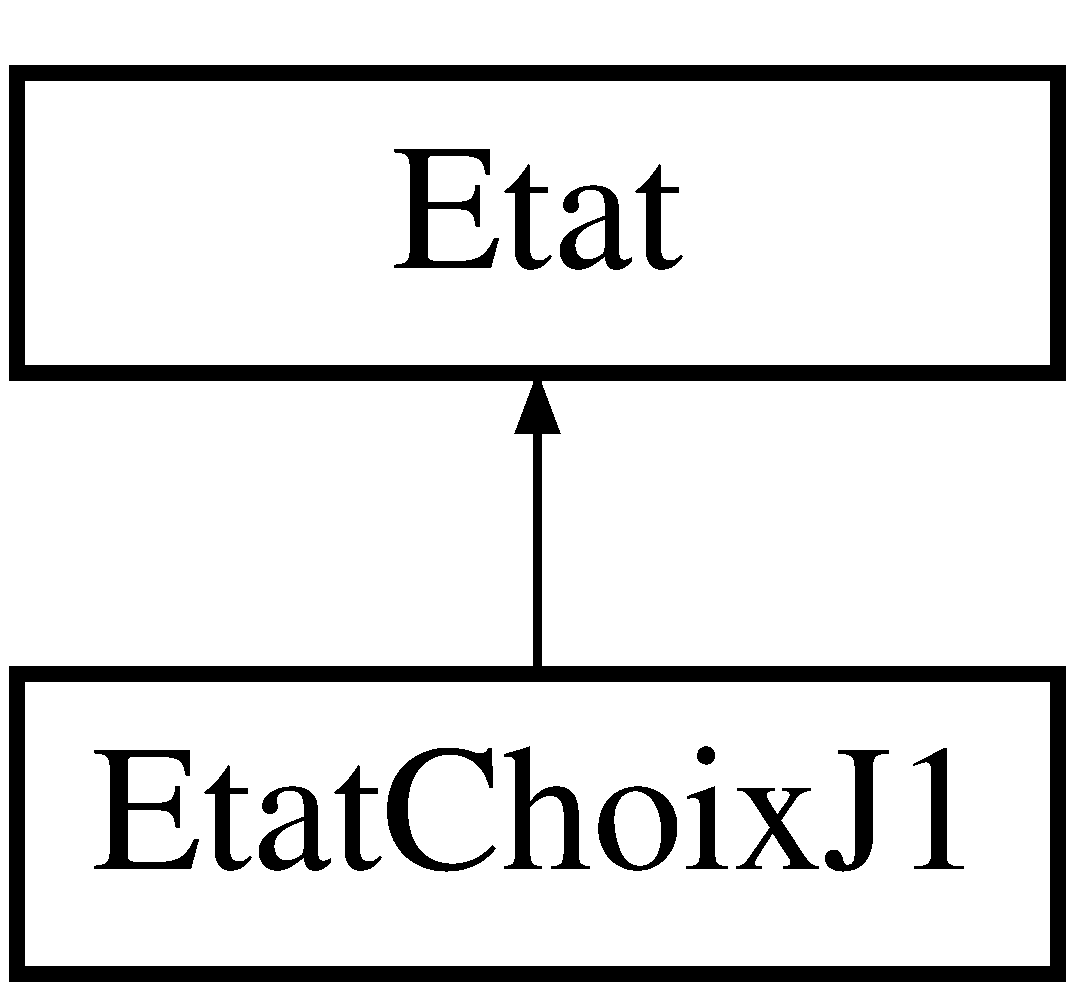
\includegraphics[height=2.000000cm]{class_etat_choix_j1}
\end{center}
\end{figure}
\subsection*{Fonctions membres publiques}
\begin{DoxyCompactItemize}
\item 
\hyperlink{class_etat_choix_j1_ad88037fd8ee0d8e2008d4af43104c7f2}{Etat\-Choix\-J1} (\hyperlink{class_jeu}{Jeu} $\ast$jeu)
\begin{DoxyCompactList}\small\item\em Constructeur. \end{DoxyCompactList}\item 
void \hyperlink{class_etat_choix_j1_afb7b74d31ac30f1993cd6ae35ff72733}{verification} ()
\begin{DoxyCompactList}\small\item\em \hyperlink{class_etat_choix_j1}{Etat\-Choix\-J1} \-: aplique les effet de la carte jouer par J1. \end{DoxyCompactList}\item 
void \hyperlink{class_etat_choix_j1_aeb4984f144a61f1a98120dc844364212}{Info\-Carte} ()
\begin{DoxyCompactList}\small\item\em \hyperlink{class_etat_choix_j1}{Etat\-Choix\-J1} \-: demande un numéro et affiche les infos de la carte corespondante dans la main du joueur 1. \end{DoxyCompactList}\item 
void \hyperlink{class_etat_choix_j1_a923857828b87f0bde7661e4f7a17efee}{retourner\-Carte} ()
\begin{DoxyCompactList}\small\item\em \hyperlink{class_etat_choix_j1}{Etat\-Choix\-J1} \-: demande un numéro et retourne la carte corespondante de la main du joueur 1. \end{DoxyCompactList}\item 
void \hyperlink{class_etat_choix_j1_a5aa86ab5766846edd95a5f82943855a1}{jouer\-Carte} ()
\begin{DoxyCompactList}\small\item\em \hyperlink{class_etat_choix_j1}{Etat\-Choix\-J1} \-: demande un numéro et joue la carte corespondante de la main du joueur 1 ( demande confirmation) \end{DoxyCompactList}\item 
void \hyperlink{class_etat_choix_j1_a7c9397632889bb66bdd5a635ab7ad3cb}{confirmation} ()
\begin{DoxyCompactList}\small\item\em \hyperlink{class_etat_choix_j1}{Etat\-Choix\-J1} \-: si le joueur 1 confirme appelle vérification et passe à l'état choix J2. \end{DoxyCompactList}\item 
void \hyperlink{class_etat_choix_j1_af6a16d04020f3079a6a02e5cae8860ec}{annuler\-Action} ()
\begin{DoxyCompactList}\small\item\em \hyperlink{class_etat_choix_j1}{Etat\-Choix\-J1} \-: si le joueur 1 ne annule son action retourne la carte qu'il vient de joueur dans sa main. \end{DoxyCompactList}\end{DoxyCompactItemize}


\subsection{Documentation des constructeurs et destructeur}
\hypertarget{class_etat_choix_j1_ad88037fd8ee0d8e2008d4af43104c7f2}{\index{Etat\-Choix\-J1@{Etat\-Choix\-J1}!Etat\-Choix\-J1@{Etat\-Choix\-J1}}
\index{Etat\-Choix\-J1@{Etat\-Choix\-J1}!EtatChoixJ1@{Etat\-Choix\-J1}}
\subsubsection[{Etat\-Choix\-J1}]{\setlength{\rightskip}{0pt plus 5cm}Etat\-Choix\-J1\-::\-Etat\-Choix\-J1 (
\begin{DoxyParamCaption}
\item[{{\bf Jeu} $\ast$}]{jeu}
\end{DoxyParamCaption}
)\hspace{0.3cm}{\ttfamily [inline]}}}\label{class_etat_choix_j1_ad88037fd8ee0d8e2008d4af43104c7f2}


Constructeur. 

Constructeur de la classe \hyperlink{class_etat_choix_j1}{Etat\-Choix\-J1}


\begin{DoxyParams}{Paramètres}
{\em jeu} & \-: pointeur vers le jeu \\
\hline
\end{DoxyParams}


\subsection{Documentation des fonctions membres}
\hypertarget{class_etat_choix_j1_af6a16d04020f3079a6a02e5cae8860ec}{\index{Etat\-Choix\-J1@{Etat\-Choix\-J1}!annuler\-Action@{annuler\-Action}}
\index{annuler\-Action@{annuler\-Action}!EtatChoixJ1@{Etat\-Choix\-J1}}
\subsubsection[{annuler\-Action}]{\setlength{\rightskip}{0pt plus 5cm}void Etat\-Choix\-J1\-::annuler\-Action (
\begin{DoxyParamCaption}
{}
\end{DoxyParamCaption}
)\hspace{0.3cm}{\ttfamily [virtual]}}}\label{class_etat_choix_j1_af6a16d04020f3079a6a02e5cae8860ec}


\hyperlink{class_etat_choix_j1}{Etat\-Choix\-J1} \-: si le joueur 1 ne annule son action retourne la carte qu'il vient de joueur dans sa main. 



Implémente \hyperlink{class_etat_ac47332db984da58192bbb1c45f1702a8}{Etat}.

\hypertarget{class_etat_choix_j1_a7c9397632889bb66bdd5a635ab7ad3cb}{\index{Etat\-Choix\-J1@{Etat\-Choix\-J1}!confirmation@{confirmation}}
\index{confirmation@{confirmation}!EtatChoixJ1@{Etat\-Choix\-J1}}
\subsubsection[{confirmation}]{\setlength{\rightskip}{0pt plus 5cm}void Etat\-Choix\-J1\-::confirmation (
\begin{DoxyParamCaption}
{}
\end{DoxyParamCaption}
)\hspace{0.3cm}{\ttfamily [virtual]}}}\label{class_etat_choix_j1_a7c9397632889bb66bdd5a635ab7ad3cb}


\hyperlink{class_etat_choix_j1}{Etat\-Choix\-J1} \-: si le joueur 1 confirme appelle vérification et passe à l'état choix J2. 



Implémente \hyperlink{class_etat_a65c2e505cda8cac2989b3a0c17a70278}{Etat}.

\hypertarget{class_etat_choix_j1_aeb4984f144a61f1a98120dc844364212}{\index{Etat\-Choix\-J1@{Etat\-Choix\-J1}!Info\-Carte@{Info\-Carte}}
\index{Info\-Carte@{Info\-Carte}!EtatChoixJ1@{Etat\-Choix\-J1}}
\subsubsection[{Info\-Carte}]{\setlength{\rightskip}{0pt plus 5cm}void Etat\-Choix\-J1\-::\-Info\-Carte (
\begin{DoxyParamCaption}
{}
\end{DoxyParamCaption}
)\hspace{0.3cm}{\ttfamily [virtual]}}}\label{class_etat_choix_j1_aeb4984f144a61f1a98120dc844364212}


\hyperlink{class_etat_choix_j1}{Etat\-Choix\-J1} \-: demande un numéro et affiche les infos de la carte corespondante dans la main du joueur 1. 



Implémente \hyperlink{class_etat_afd99ba60265bc0a82029d5fa2368acfa}{Etat}.

\hypertarget{class_etat_choix_j1_a5aa86ab5766846edd95a5f82943855a1}{\index{Etat\-Choix\-J1@{Etat\-Choix\-J1}!jouer\-Carte@{jouer\-Carte}}
\index{jouer\-Carte@{jouer\-Carte}!EtatChoixJ1@{Etat\-Choix\-J1}}
\subsubsection[{jouer\-Carte}]{\setlength{\rightskip}{0pt plus 5cm}void Etat\-Choix\-J1\-::jouer\-Carte (
\begin{DoxyParamCaption}
{}
\end{DoxyParamCaption}
)\hspace{0.3cm}{\ttfamily [virtual]}}}\label{class_etat_choix_j1_a5aa86ab5766846edd95a5f82943855a1}


\hyperlink{class_etat_choix_j1}{Etat\-Choix\-J1} \-: demande un numéro et joue la carte corespondante de la main du joueur 1 ( demande confirmation) 



Implémente \hyperlink{class_etat_aaeffe08c27b2b64560726f5df95e6f3a}{Etat}.

\hypertarget{class_etat_choix_j1_a923857828b87f0bde7661e4f7a17efee}{\index{Etat\-Choix\-J1@{Etat\-Choix\-J1}!retourner\-Carte@{retourner\-Carte}}
\index{retourner\-Carte@{retourner\-Carte}!EtatChoixJ1@{Etat\-Choix\-J1}}
\subsubsection[{retourner\-Carte}]{\setlength{\rightskip}{0pt plus 5cm}void Etat\-Choix\-J1\-::retourner\-Carte (
\begin{DoxyParamCaption}
{}
\end{DoxyParamCaption}
)\hspace{0.3cm}{\ttfamily [virtual]}}}\label{class_etat_choix_j1_a923857828b87f0bde7661e4f7a17efee}


\hyperlink{class_etat_choix_j1}{Etat\-Choix\-J1} \-: demande un numéro et retourne la carte corespondante de la main du joueur 1. 



Implémente \hyperlink{class_etat_a3d2fe662ffd20147763a25c4e06b56e9}{Etat}.

\hypertarget{class_etat_choix_j1_afb7b74d31ac30f1993cd6ae35ff72733}{\index{Etat\-Choix\-J1@{Etat\-Choix\-J1}!verification@{verification}}
\index{verification@{verification}!EtatChoixJ1@{Etat\-Choix\-J1}}
\subsubsection[{verification}]{\setlength{\rightskip}{0pt plus 5cm}void Etat\-Choix\-J1\-::verification (
\begin{DoxyParamCaption}
{}
\end{DoxyParamCaption}
)\hspace{0.3cm}{\ttfamily [virtual]}}}\label{class_etat_choix_j1_afb7b74d31ac30f1993cd6ae35ff72733}


\hyperlink{class_etat_choix_j1}{Etat\-Choix\-J1} \-: aplique les effet de la carte jouer par J1. 



Implémente \hyperlink{class_etat_aaf949c7b45217b76ff68414e61ef0d2a}{Etat}.



La documentation de cette classe a été générée à partir du fichier suivant \-:\begin{DoxyCompactItemize}
\item 
/home/figiel-\/paul/\-Bureau/\-Projet\-Poo/\-Projet\-P\-O\-O-\/\-A\-R\-A\-Y\-A-\/\-F\-I\-G\-I\-E\-L/include/\hyperlink{_etat_choix_j1_8hpp}{Etat\-Choix\-J1.\-hpp}\end{DoxyCompactItemize}

\hypertarget{class_etat_choix_j2}{\section{Référence de la classe Etat\-Choix\-J2}
\label{class_etat_choix_j2}\index{Etat\-Choix\-J2@{Etat\-Choix\-J2}}
}


{\ttfamily \#include $<$Etat\-Choix\-J2.\-hpp$>$}

Graphe d'héritage de Etat\-Choix\-J2\-:\begin{figure}[H]
\begin{center}
\leavevmode
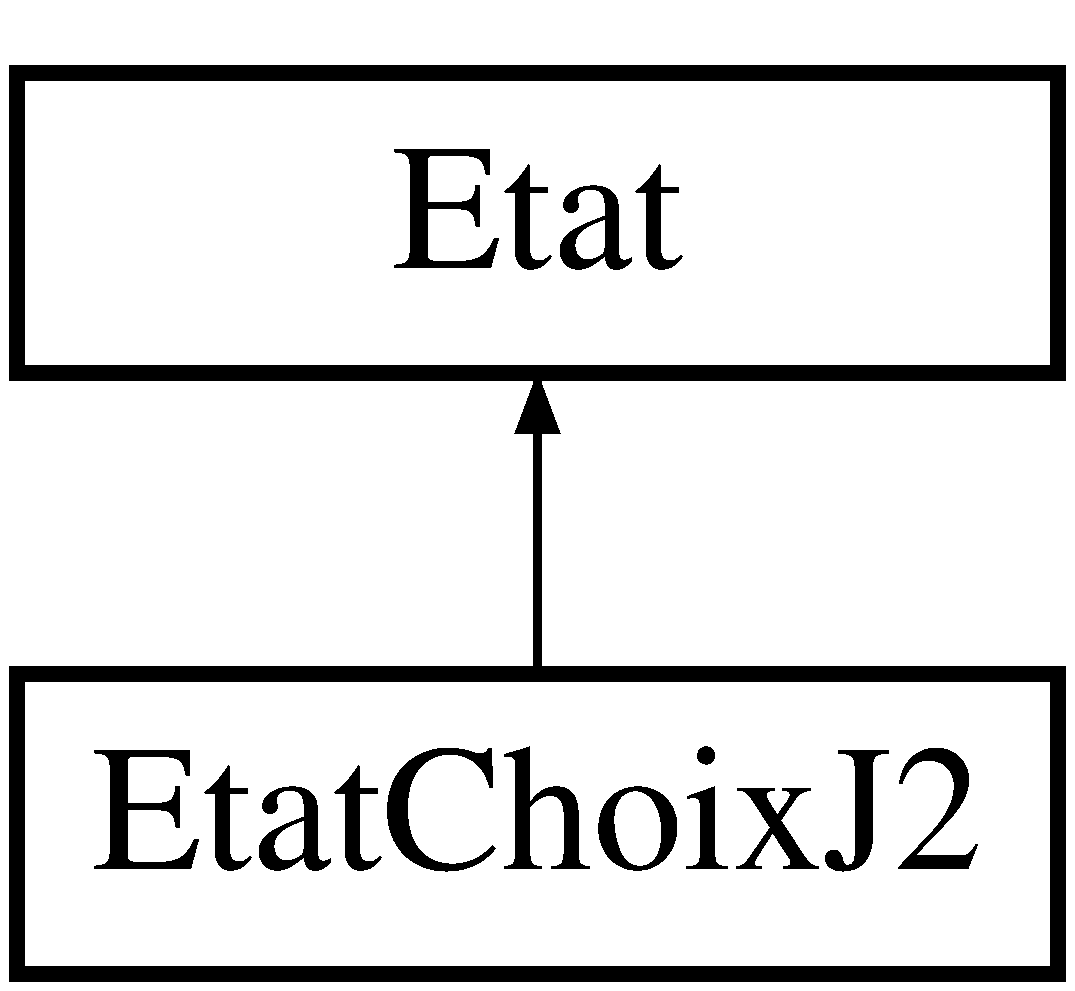
\includegraphics[height=2.000000cm]{class_etat_choix_j2}
\end{center}
\end{figure}
\subsection*{Fonctions membres publiques}
\begin{DoxyCompactItemize}
\item 
\hyperlink{class_etat_choix_j2_a03b6c1b78ae155873b16335eaba68ea7}{Etat\-Choix\-J2} (\hyperlink{class_jeu}{Jeu} $\ast$jeu)
\begin{DoxyCompactList}\small\item\em Constructeur. \end{DoxyCompactList}\item 
void \hyperlink{class_etat_choix_j2_a93667fd195d816e8d3e8e26d16a86848}{verification} ()
\begin{DoxyCompactList}\small\item\em \hyperlink{class_etat_choix_j2}{Etat\-Choix\-J2} \-: aplique les effet de la carte jouer par J2. \end{DoxyCompactList}\item 
void \hyperlink{class_etat_choix_j2_ab0066e2aa95ddfe577d0e9ba4ae5441e}{Info\-Carte} ()
\begin{DoxyCompactList}\small\item\em \hyperlink{class_etat_choix_j2}{Etat\-Choix\-J2} \-: demande un numéro et affiche les infos de la carte corespondante dans la main du joueur 2. \end{DoxyCompactList}\item 
void \hyperlink{class_etat_choix_j2_a2fe8000154f582684c9a0162bb860b9f}{retourner\-Carte} ()
\begin{DoxyCompactList}\small\item\em \hyperlink{class_etat_choix_j2}{Etat\-Choix\-J2} \-: demande un numéro et retourne la carte corespondante de la main du joueur 2. \end{DoxyCompactList}\item 
void \hyperlink{class_etat_choix_j2_a674ef9e896f33d70cf8937b4591faae9}{jouer\-Carte} ()
\begin{DoxyCompactList}\small\item\em \hyperlink{class_etat_choix_j2}{Etat\-Choix\-J2} \-: demande un numéro et joue la carte corespondante de la main du joueur 2 ( demande confirmation) \end{DoxyCompactList}\item 
void \hyperlink{class_etat_choix_j2_af09ee4f38957e7fe8232db7dcfccd573}{confirmation} ()
\begin{DoxyCompactList}\small\item\em \hyperlink{class_etat_choix_j2}{Etat\-Choix\-J2} \-: si le joueur 2 confirme appelle vérification et passe à \hyperlink{class_etat_choix_win}{Etat\-Choix\-Win}. \end{DoxyCompactList}\item 
void \hyperlink{class_etat_choix_j2_a076a02ef80e3dded9fb3df17dd23542a}{annuler\-Action} ()
\begin{DoxyCompactList}\small\item\em \hyperlink{class_etat_choix_j2}{Etat\-Choix\-J2} \-: si le joueur 2 ne annule son action retourne la carte qu'il vient de joueur dans sa main. \end{DoxyCompactList}\end{DoxyCompactItemize}


\subsection{Documentation des constructeurs et destructeur}
\hypertarget{class_etat_choix_j2_a03b6c1b78ae155873b16335eaba68ea7}{\index{Etat\-Choix\-J2@{Etat\-Choix\-J2}!Etat\-Choix\-J2@{Etat\-Choix\-J2}}
\index{Etat\-Choix\-J2@{Etat\-Choix\-J2}!EtatChoixJ2@{Etat\-Choix\-J2}}
\subsubsection[{Etat\-Choix\-J2}]{\setlength{\rightskip}{0pt plus 5cm}Etat\-Choix\-J2\-::\-Etat\-Choix\-J2 (
\begin{DoxyParamCaption}
\item[{{\bf Jeu} $\ast$}]{jeu}
\end{DoxyParamCaption}
)\hspace{0.3cm}{\ttfamily [inline]}}}\label{class_etat_choix_j2_a03b6c1b78ae155873b16335eaba68ea7}


Constructeur. 

Constructeur de la classe \hyperlink{class_etat_choix_j2}{Etat\-Choix\-J2}


\begin{DoxyParams}{Paramètres}
{\em jeu} & \-: pointeur vers le jeu \\
\hline
\end{DoxyParams}


\subsection{Documentation des fonctions membres}
\hypertarget{class_etat_choix_j2_a076a02ef80e3dded9fb3df17dd23542a}{\index{Etat\-Choix\-J2@{Etat\-Choix\-J2}!annuler\-Action@{annuler\-Action}}
\index{annuler\-Action@{annuler\-Action}!EtatChoixJ2@{Etat\-Choix\-J2}}
\subsubsection[{annuler\-Action}]{\setlength{\rightskip}{0pt plus 5cm}void Etat\-Choix\-J2\-::annuler\-Action (
\begin{DoxyParamCaption}
{}
\end{DoxyParamCaption}
)\hspace{0.3cm}{\ttfamily [virtual]}}}\label{class_etat_choix_j2_a076a02ef80e3dded9fb3df17dd23542a}


\hyperlink{class_etat_choix_j2}{Etat\-Choix\-J2} \-: si le joueur 2 ne annule son action retourne la carte qu'il vient de joueur dans sa main. 



Implémente \hyperlink{class_etat_ac47332db984da58192bbb1c45f1702a8}{Etat}.

\hypertarget{class_etat_choix_j2_af09ee4f38957e7fe8232db7dcfccd573}{\index{Etat\-Choix\-J2@{Etat\-Choix\-J2}!confirmation@{confirmation}}
\index{confirmation@{confirmation}!EtatChoixJ2@{Etat\-Choix\-J2}}
\subsubsection[{confirmation}]{\setlength{\rightskip}{0pt plus 5cm}void Etat\-Choix\-J2\-::confirmation (
\begin{DoxyParamCaption}
{}
\end{DoxyParamCaption}
)\hspace{0.3cm}{\ttfamily [virtual]}}}\label{class_etat_choix_j2_af09ee4f38957e7fe8232db7dcfccd573}


\hyperlink{class_etat_choix_j2}{Etat\-Choix\-J2} \-: si le joueur 2 confirme appelle vérification et passe à \hyperlink{class_etat_choix_win}{Etat\-Choix\-Win}. 



Implémente \hyperlink{class_etat_a65c2e505cda8cac2989b3a0c17a70278}{Etat}.

\hypertarget{class_etat_choix_j2_ab0066e2aa95ddfe577d0e9ba4ae5441e}{\index{Etat\-Choix\-J2@{Etat\-Choix\-J2}!Info\-Carte@{Info\-Carte}}
\index{Info\-Carte@{Info\-Carte}!EtatChoixJ2@{Etat\-Choix\-J2}}
\subsubsection[{Info\-Carte}]{\setlength{\rightskip}{0pt plus 5cm}void Etat\-Choix\-J2\-::\-Info\-Carte (
\begin{DoxyParamCaption}
{}
\end{DoxyParamCaption}
)\hspace{0.3cm}{\ttfamily [virtual]}}}\label{class_etat_choix_j2_ab0066e2aa95ddfe577d0e9ba4ae5441e}


\hyperlink{class_etat_choix_j2}{Etat\-Choix\-J2} \-: demande un numéro et affiche les infos de la carte corespondante dans la main du joueur 2. 



Implémente \hyperlink{class_etat_afd99ba60265bc0a82029d5fa2368acfa}{Etat}.

\hypertarget{class_etat_choix_j2_a674ef9e896f33d70cf8937b4591faae9}{\index{Etat\-Choix\-J2@{Etat\-Choix\-J2}!jouer\-Carte@{jouer\-Carte}}
\index{jouer\-Carte@{jouer\-Carte}!EtatChoixJ2@{Etat\-Choix\-J2}}
\subsubsection[{jouer\-Carte}]{\setlength{\rightskip}{0pt plus 5cm}void Etat\-Choix\-J2\-::jouer\-Carte (
\begin{DoxyParamCaption}
{}
\end{DoxyParamCaption}
)\hspace{0.3cm}{\ttfamily [virtual]}}}\label{class_etat_choix_j2_a674ef9e896f33d70cf8937b4591faae9}


\hyperlink{class_etat_choix_j2}{Etat\-Choix\-J2} \-: demande un numéro et joue la carte corespondante de la main du joueur 2 ( demande confirmation) 



Implémente \hyperlink{class_etat_aaeffe08c27b2b64560726f5df95e6f3a}{Etat}.

\hypertarget{class_etat_choix_j2_a2fe8000154f582684c9a0162bb860b9f}{\index{Etat\-Choix\-J2@{Etat\-Choix\-J2}!retourner\-Carte@{retourner\-Carte}}
\index{retourner\-Carte@{retourner\-Carte}!EtatChoixJ2@{Etat\-Choix\-J2}}
\subsubsection[{retourner\-Carte}]{\setlength{\rightskip}{0pt plus 5cm}void Etat\-Choix\-J2\-::retourner\-Carte (
\begin{DoxyParamCaption}
{}
\end{DoxyParamCaption}
)\hspace{0.3cm}{\ttfamily [virtual]}}}\label{class_etat_choix_j2_a2fe8000154f582684c9a0162bb860b9f}


\hyperlink{class_etat_choix_j2}{Etat\-Choix\-J2} \-: demande un numéro et retourne la carte corespondante de la main du joueur 2. 



Implémente \hyperlink{class_etat_a3d2fe662ffd20147763a25c4e06b56e9}{Etat}.

\hypertarget{class_etat_choix_j2_a93667fd195d816e8d3e8e26d16a86848}{\index{Etat\-Choix\-J2@{Etat\-Choix\-J2}!verification@{verification}}
\index{verification@{verification}!EtatChoixJ2@{Etat\-Choix\-J2}}
\subsubsection[{verification}]{\setlength{\rightskip}{0pt plus 5cm}void Etat\-Choix\-J2\-::verification (
\begin{DoxyParamCaption}
{}
\end{DoxyParamCaption}
)\hspace{0.3cm}{\ttfamily [virtual]}}}\label{class_etat_choix_j2_a93667fd195d816e8d3e8e26d16a86848}


\hyperlink{class_etat_choix_j2}{Etat\-Choix\-J2} \-: aplique les effet de la carte jouer par J2. 



Implémente \hyperlink{class_etat_aaf949c7b45217b76ff68414e61ef0d2a}{Etat}.



La documentation de cette classe a été générée à partir du fichier suivant \-:\begin{DoxyCompactItemize}
\item 
/home/figiel-\/paul/\-Bureau/\-Projet\-Poo/\-Projet\-P\-O\-O-\/\-A\-R\-A\-Y\-A-\/\-F\-I\-G\-I\-E\-L/include/\hyperlink{_etat_choix_j2_8hpp}{Etat\-Choix\-J2.\-hpp}\end{DoxyCompactItemize}

\hypertarget{class_etat_choix_perso}{\section{Référence de la classe Etat\-Choix\-Perso}
\label{class_etat_choix_perso}\index{Etat\-Choix\-Perso@{Etat\-Choix\-Perso}}
}


{\ttfamily \#include $<$Etat\-Choix\-Perso.\-hpp$>$}

Graphe d'héritage de Etat\-Choix\-Perso\-:\begin{figure}[H]
\begin{center}
\leavevmode
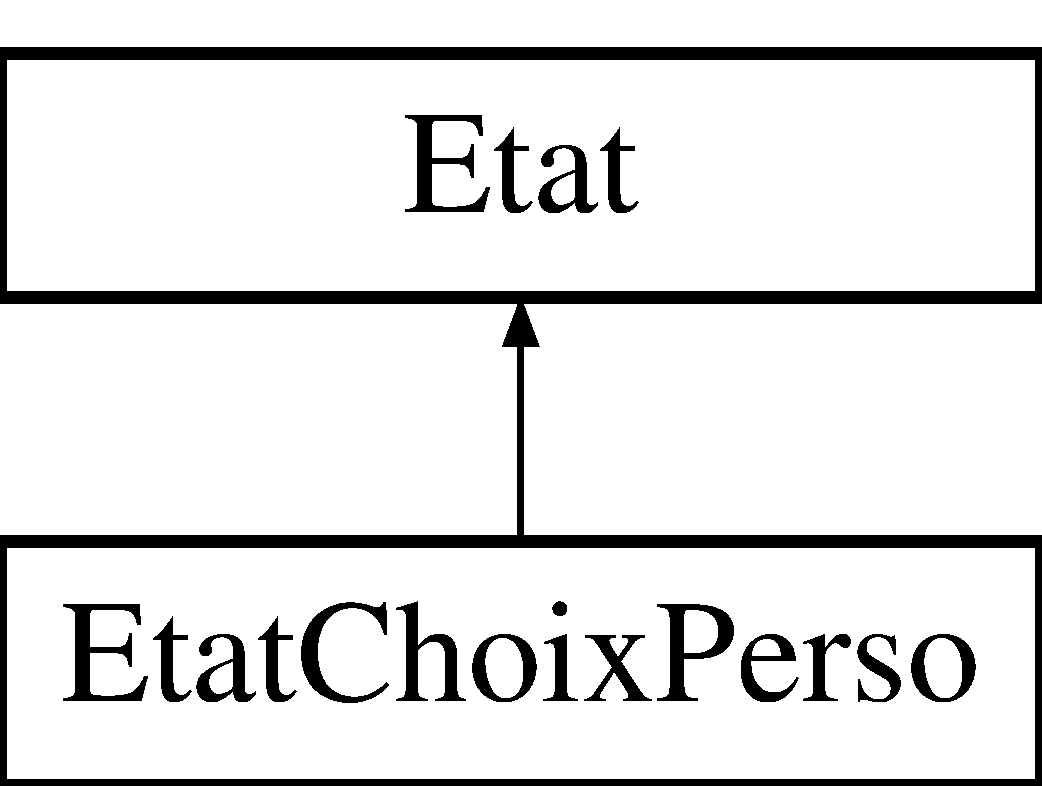
\includegraphics[height=2.000000cm]{class_etat_choix_perso}
\end{center}
\end{figure}
\subsection*{Fonctions membres publiques}
\begin{DoxyCompactItemize}
\item 
\hyperlink{class_etat_choix_perso_a95d459d52f71990384b6284739c0700e}{Etat\-Choix\-Perso} (\hyperlink{class_jeu}{Jeu} $\ast$jeu)
\item 
void \hyperlink{class_etat_choix_perso_a18678f06f60115999dd92b8b88dbe7dd}{verification} ()
\begin{DoxyCompactList}\small\item\em procéde au diverse vérification (varie selon l'état). \end{DoxyCompactList}\item 
void \hyperlink{class_etat_choix_perso_a10dcb32108b4d457bd58ad45abf6706a}{Info\-Carte} ()
\begin{DoxyCompactList}\small\item\em affiche l'info d'une carte (varie selon l'état). \end{DoxyCompactList}\item 
void \hyperlink{class_etat_choix_perso_a5a9e8efb87e8ebb31c0f4db269e938a9}{retourner\-Carte} ()
\begin{DoxyCompactList}\small\item\em retourne la dérnière carte jouer dans la main de son propriétaire (varie selon l'état). \end{DoxyCompactList}\item 
void \hyperlink{class_etat_choix_perso_a31908b4127aeff26b214d470ef22eacb}{jouer\-Carte} ()
\begin{DoxyCompactList}\small\item\em joue une carte (varie selon l'état). \end{DoxyCompactList}\item 
void \hyperlink{class_etat_choix_perso_a60ea227168029d7741f2919d73b8d2cc}{confirmation} ()
\begin{DoxyCompactList}\small\item\em confirme l'action (varie selon l'état). \end{DoxyCompactList}\item 
void \hyperlink{class_etat_choix_perso_a1a67ae6bf8cf6cd9c79afd84b1961385}{annuler\-Action} ()
\begin{DoxyCompactList}\small\item\em annule l'action (varie selon l'état). \end{DoxyCompactList}\end{DoxyCompactItemize}


\subsection{Documentation des constructeurs et destructeur}
\hypertarget{class_etat_choix_perso_a95d459d52f71990384b6284739c0700e}{\index{Etat\-Choix\-Perso@{Etat\-Choix\-Perso}!Etat\-Choix\-Perso@{Etat\-Choix\-Perso}}
\index{Etat\-Choix\-Perso@{Etat\-Choix\-Perso}!EtatChoixPerso@{Etat\-Choix\-Perso}}
\subsubsection[{Etat\-Choix\-Perso}]{\setlength{\rightskip}{0pt plus 5cm}Etat\-Choix\-Perso\-::\-Etat\-Choix\-Perso (
\begin{DoxyParamCaption}
\item[{{\bf Jeu} $\ast$}]{jeu}
\end{DoxyParamCaption}
)\hspace{0.3cm}{\ttfamily [inline]}}}\label{class_etat_choix_perso_a95d459d52f71990384b6284739c0700e}


\subsection{Documentation des fonctions membres}
\hypertarget{class_etat_choix_perso_a1a67ae6bf8cf6cd9c79afd84b1961385}{\index{Etat\-Choix\-Perso@{Etat\-Choix\-Perso}!annuler\-Action@{annuler\-Action}}
\index{annuler\-Action@{annuler\-Action}!EtatChoixPerso@{Etat\-Choix\-Perso}}
\subsubsection[{annuler\-Action}]{\setlength{\rightskip}{0pt plus 5cm}void Etat\-Choix\-Perso\-::annuler\-Action (
\begin{DoxyParamCaption}
{}
\end{DoxyParamCaption}
)\hspace{0.3cm}{\ttfamily [virtual]}}}\label{class_etat_choix_perso_a1a67ae6bf8cf6cd9c79afd84b1961385}


annule l'action (varie selon l'état). 



Implémente \hyperlink{class_etat_ac47332db984da58192bbb1c45f1702a8}{Etat}.

\hypertarget{class_etat_choix_perso_a60ea227168029d7741f2919d73b8d2cc}{\index{Etat\-Choix\-Perso@{Etat\-Choix\-Perso}!confirmation@{confirmation}}
\index{confirmation@{confirmation}!EtatChoixPerso@{Etat\-Choix\-Perso}}
\subsubsection[{confirmation}]{\setlength{\rightskip}{0pt plus 5cm}void Etat\-Choix\-Perso\-::confirmation (
\begin{DoxyParamCaption}
{}
\end{DoxyParamCaption}
)\hspace{0.3cm}{\ttfamily [virtual]}}}\label{class_etat_choix_perso_a60ea227168029d7741f2919d73b8d2cc}


confirme l'action (varie selon l'état). 



Implémente \hyperlink{class_etat_a65c2e505cda8cac2989b3a0c17a70278}{Etat}.

\hypertarget{class_etat_choix_perso_a10dcb32108b4d457bd58ad45abf6706a}{\index{Etat\-Choix\-Perso@{Etat\-Choix\-Perso}!Info\-Carte@{Info\-Carte}}
\index{Info\-Carte@{Info\-Carte}!EtatChoixPerso@{Etat\-Choix\-Perso}}
\subsubsection[{Info\-Carte}]{\setlength{\rightskip}{0pt plus 5cm}void Etat\-Choix\-Perso\-::\-Info\-Carte (
\begin{DoxyParamCaption}
{}
\end{DoxyParamCaption}
)\hspace{0.3cm}{\ttfamily [virtual]}}}\label{class_etat_choix_perso_a10dcb32108b4d457bd58ad45abf6706a}


affiche l'info d'une carte (varie selon l'état). 



Implémente \hyperlink{class_etat_afd99ba60265bc0a82029d5fa2368acfa}{Etat}.

\hypertarget{class_etat_choix_perso_a31908b4127aeff26b214d470ef22eacb}{\index{Etat\-Choix\-Perso@{Etat\-Choix\-Perso}!jouer\-Carte@{jouer\-Carte}}
\index{jouer\-Carte@{jouer\-Carte}!EtatChoixPerso@{Etat\-Choix\-Perso}}
\subsubsection[{jouer\-Carte}]{\setlength{\rightskip}{0pt plus 5cm}void Etat\-Choix\-Perso\-::jouer\-Carte (
\begin{DoxyParamCaption}
{}
\end{DoxyParamCaption}
)\hspace{0.3cm}{\ttfamily [virtual]}}}\label{class_etat_choix_perso_a31908b4127aeff26b214d470ef22eacb}


joue une carte (varie selon l'état). 



Implémente \hyperlink{class_etat_aaeffe08c27b2b64560726f5df95e6f3a}{Etat}.

\hypertarget{class_etat_choix_perso_a5a9e8efb87e8ebb31c0f4db269e938a9}{\index{Etat\-Choix\-Perso@{Etat\-Choix\-Perso}!retourner\-Carte@{retourner\-Carte}}
\index{retourner\-Carte@{retourner\-Carte}!EtatChoixPerso@{Etat\-Choix\-Perso}}
\subsubsection[{retourner\-Carte}]{\setlength{\rightskip}{0pt plus 5cm}void Etat\-Choix\-Perso\-::retourner\-Carte (
\begin{DoxyParamCaption}
{}
\end{DoxyParamCaption}
)\hspace{0.3cm}{\ttfamily [virtual]}}}\label{class_etat_choix_perso_a5a9e8efb87e8ebb31c0f4db269e938a9}


retourne la dérnière carte jouer dans la main de son propriétaire (varie selon l'état). 



Implémente \hyperlink{class_etat_a3d2fe662ffd20147763a25c4e06b56e9}{Etat}.

\hypertarget{class_etat_choix_perso_a18678f06f60115999dd92b8b88dbe7dd}{\index{Etat\-Choix\-Perso@{Etat\-Choix\-Perso}!verification@{verification}}
\index{verification@{verification}!EtatChoixPerso@{Etat\-Choix\-Perso}}
\subsubsection[{verification}]{\setlength{\rightskip}{0pt plus 5cm}void Etat\-Choix\-Perso\-::verification (
\begin{DoxyParamCaption}
{}
\end{DoxyParamCaption}
)\hspace{0.3cm}{\ttfamily [virtual]}}}\label{class_etat_choix_perso_a18678f06f60115999dd92b8b88dbe7dd}


procéde au diverse vérification (varie selon l'état). 



Implémente \hyperlink{class_etat_aaf949c7b45217b76ff68414e61ef0d2a}{Etat}.



La documentation de cette classe a été générée à partir du fichier suivant \-:\begin{DoxyCompactItemize}
\item 
/home/figiel-\/paul/\-Bureau/\-Projet\-Poo/\-Projet\-P\-O\-O-\/\-A\-R\-A\-Y\-A-\/\-F\-I\-G\-I\-E\-L/include/\hyperlink{_etat_choix_perso_8hpp}{Etat\-Choix\-Perso.\-hpp}\end{DoxyCompactItemize}

\hypertarget{class_etat_choix_win}{\section{Référence de la classe Etat\-Choix\-Win}
\label{class_etat_choix_win}\index{Etat\-Choix\-Win@{Etat\-Choix\-Win}}
}


{\ttfamily \#include $<$Etat\-Choix\-Win.\-hpp$>$}

Graphe d'héritage de Etat\-Choix\-Win\-:\begin{figure}[H]
\begin{center}
\leavevmode
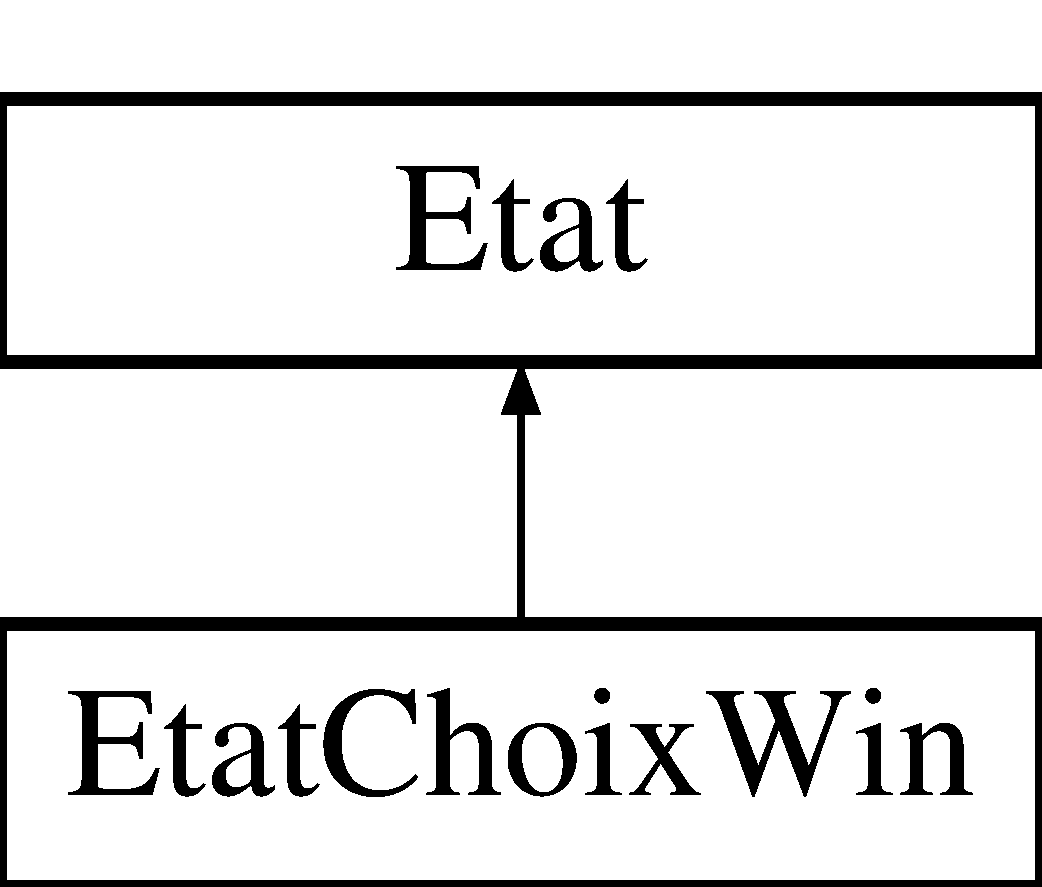
\includegraphics[height=2.000000cm]{class_etat_choix_win}
\end{center}
\end{figure}
\subsection*{Fonctions membres publiques}
\begin{DoxyCompactItemize}
\item 
\hyperlink{class_etat_choix_win_a3b9cb41872f4cc11aa52cd22b62de7c3}{Etat\-Choix\-Win} (\hyperlink{class_jeu}{Jeu} $\ast$jeu)
\begin{DoxyCompactList}\small\item\em Constructeur. \end{DoxyCompactList}\item 
void \hyperlink{class_etat_choix_win_ae4b933e5eb219ad05263447db0d970e2}{verification} ()
\begin{DoxyCompactList}\small\item\em \hyperlink{class_etat_choix_win}{Etat\-Choix\-Win} \-: procédè à toutes les vérification nécessaire et décide du gagnant du combat. Envoie vers \hyperlink{class_etat_bluff}{Etat\-Bluff}, \hyperlink{class_etat_calc_dmg}{Etat\-Calc\-Dmg}, \hyperlink{class_etat_clean_up}{Etat\-Clean\-Up} selpn les cas. \end{DoxyCompactList}\item 
void \hyperlink{class_etat_choix_win_af5143e3b6e6c80633b48fcbc9fa52be2}{Info\-Carte} ()
\begin{DoxyCompactList}\small\item\em \hyperlink{class_etat_choix_win}{Etat\-Choix\-Win}\-:pas d'effet. \end{DoxyCompactList}\item 
void \hyperlink{class_etat_choix_win_a583e3a7b7d7e922a74a4609d31c277ee}{retourner\-Carte} ()
\begin{DoxyCompactList}\small\item\em \hyperlink{class_etat_choix_win}{Etat\-Choix\-Win}\-:pas d'effet. \end{DoxyCompactList}\item 
void \hyperlink{class_etat_choix_win_a32f02c55bfbf8b580dee3bd95ce1921e}{jouer\-Carte} ()
\begin{DoxyCompactList}\small\item\em \hyperlink{class_etat_choix_win}{Etat\-Choix\-Win}\-:pas d'effet. \end{DoxyCompactList}\item 
void \hyperlink{class_etat_choix_win_aef8d0abe059050e7a7e3e598c87de992}{confirmation} ()
\begin{DoxyCompactList}\small\item\em \hyperlink{class_etat_choix_win}{Etat\-Choix\-Win}\-:pas d'effet. \end{DoxyCompactList}\item 
void \hyperlink{class_etat_choix_win_ae321052d630a6a679f6347c36f580ea7}{annuler\-Action} ()
\begin{DoxyCompactList}\small\item\em \hyperlink{class_etat_choix_win}{Etat\-Choix\-Win}\-:pas d'effet. \end{DoxyCompactList}\end{DoxyCompactItemize}


\subsection{Documentation des constructeurs et destructeur}
\hypertarget{class_etat_choix_win_a3b9cb41872f4cc11aa52cd22b62de7c3}{\index{Etat\-Choix\-Win@{Etat\-Choix\-Win}!Etat\-Choix\-Win@{Etat\-Choix\-Win}}
\index{Etat\-Choix\-Win@{Etat\-Choix\-Win}!EtatChoixWin@{Etat\-Choix\-Win}}
\subsubsection[{Etat\-Choix\-Win}]{\setlength{\rightskip}{0pt plus 5cm}Etat\-Choix\-Win\-::\-Etat\-Choix\-Win (
\begin{DoxyParamCaption}
\item[{{\bf Jeu} $\ast$}]{jeu}
\end{DoxyParamCaption}
)\hspace{0.3cm}{\ttfamily [inline]}}}\label{class_etat_choix_win_a3b9cb41872f4cc11aa52cd22b62de7c3}


Constructeur. 

Constructeur de la classe \hyperlink{class_etat_choix_win}{Etat\-Choix\-Win}


\begin{DoxyParams}{Paramètres}
{\em jeu} & \-: pointeur vers le jeu \\
\hline
\end{DoxyParams}


\subsection{Documentation des fonctions membres}
\hypertarget{class_etat_choix_win_ae321052d630a6a679f6347c36f580ea7}{\index{Etat\-Choix\-Win@{Etat\-Choix\-Win}!annuler\-Action@{annuler\-Action}}
\index{annuler\-Action@{annuler\-Action}!EtatChoixWin@{Etat\-Choix\-Win}}
\subsubsection[{annuler\-Action}]{\setlength{\rightskip}{0pt plus 5cm}void Etat\-Choix\-Win\-::annuler\-Action (
\begin{DoxyParamCaption}
{}
\end{DoxyParamCaption}
)\hspace{0.3cm}{\ttfamily [virtual]}}}\label{class_etat_choix_win_ae321052d630a6a679f6347c36f580ea7}


\hyperlink{class_etat_choix_win}{Etat\-Choix\-Win}\-:pas d'effet. 



Implémente \hyperlink{class_etat_ac47332db984da58192bbb1c45f1702a8}{Etat}.

\hypertarget{class_etat_choix_win_aef8d0abe059050e7a7e3e598c87de992}{\index{Etat\-Choix\-Win@{Etat\-Choix\-Win}!confirmation@{confirmation}}
\index{confirmation@{confirmation}!EtatChoixWin@{Etat\-Choix\-Win}}
\subsubsection[{confirmation}]{\setlength{\rightskip}{0pt plus 5cm}void Etat\-Choix\-Win\-::confirmation (
\begin{DoxyParamCaption}
{}
\end{DoxyParamCaption}
)\hspace{0.3cm}{\ttfamily [virtual]}}}\label{class_etat_choix_win_aef8d0abe059050e7a7e3e598c87de992}


\hyperlink{class_etat_choix_win}{Etat\-Choix\-Win}\-:pas d'effet. 



Implémente \hyperlink{class_etat_a65c2e505cda8cac2989b3a0c17a70278}{Etat}.

\hypertarget{class_etat_choix_win_af5143e3b6e6c80633b48fcbc9fa52be2}{\index{Etat\-Choix\-Win@{Etat\-Choix\-Win}!Info\-Carte@{Info\-Carte}}
\index{Info\-Carte@{Info\-Carte}!EtatChoixWin@{Etat\-Choix\-Win}}
\subsubsection[{Info\-Carte}]{\setlength{\rightskip}{0pt plus 5cm}void Etat\-Choix\-Win\-::\-Info\-Carte (
\begin{DoxyParamCaption}
{}
\end{DoxyParamCaption}
)\hspace{0.3cm}{\ttfamily [virtual]}}}\label{class_etat_choix_win_af5143e3b6e6c80633b48fcbc9fa52be2}


\hyperlink{class_etat_choix_win}{Etat\-Choix\-Win}\-:pas d'effet. 



Implémente \hyperlink{class_etat_afd99ba60265bc0a82029d5fa2368acfa}{Etat}.

\hypertarget{class_etat_choix_win_a32f02c55bfbf8b580dee3bd95ce1921e}{\index{Etat\-Choix\-Win@{Etat\-Choix\-Win}!jouer\-Carte@{jouer\-Carte}}
\index{jouer\-Carte@{jouer\-Carte}!EtatChoixWin@{Etat\-Choix\-Win}}
\subsubsection[{jouer\-Carte}]{\setlength{\rightskip}{0pt plus 5cm}void Etat\-Choix\-Win\-::jouer\-Carte (
\begin{DoxyParamCaption}
{}
\end{DoxyParamCaption}
)\hspace{0.3cm}{\ttfamily [virtual]}}}\label{class_etat_choix_win_a32f02c55bfbf8b580dee3bd95ce1921e}


\hyperlink{class_etat_choix_win}{Etat\-Choix\-Win}\-:pas d'effet. 



Implémente \hyperlink{class_etat_aaeffe08c27b2b64560726f5df95e6f3a}{Etat}.

\hypertarget{class_etat_choix_win_a583e3a7b7d7e922a74a4609d31c277ee}{\index{Etat\-Choix\-Win@{Etat\-Choix\-Win}!retourner\-Carte@{retourner\-Carte}}
\index{retourner\-Carte@{retourner\-Carte}!EtatChoixWin@{Etat\-Choix\-Win}}
\subsubsection[{retourner\-Carte}]{\setlength{\rightskip}{0pt plus 5cm}void Etat\-Choix\-Win\-::retourner\-Carte (
\begin{DoxyParamCaption}
{}
\end{DoxyParamCaption}
)\hspace{0.3cm}{\ttfamily [virtual]}}}\label{class_etat_choix_win_a583e3a7b7d7e922a74a4609d31c277ee}


\hyperlink{class_etat_choix_win}{Etat\-Choix\-Win}\-:pas d'effet. 



Implémente \hyperlink{class_etat_a3d2fe662ffd20147763a25c4e06b56e9}{Etat}.

\hypertarget{class_etat_choix_win_ae4b933e5eb219ad05263447db0d970e2}{\index{Etat\-Choix\-Win@{Etat\-Choix\-Win}!verification@{verification}}
\index{verification@{verification}!EtatChoixWin@{Etat\-Choix\-Win}}
\subsubsection[{verification}]{\setlength{\rightskip}{0pt plus 5cm}void Etat\-Choix\-Win\-::verification (
\begin{DoxyParamCaption}
{}
\end{DoxyParamCaption}
)\hspace{0.3cm}{\ttfamily [virtual]}}}\label{class_etat_choix_win_ae4b933e5eb219ad05263447db0d970e2}


\hyperlink{class_etat_choix_win}{Etat\-Choix\-Win} \-: procédè à toutes les vérification nécessaire et décide du gagnant du combat. Envoie vers \hyperlink{class_etat_bluff}{Etat\-Bluff}, \hyperlink{class_etat_calc_dmg}{Etat\-Calc\-Dmg}, \hyperlink{class_etat_clean_up}{Etat\-Clean\-Up} selpn les cas. 



Implémente \hyperlink{class_etat_aaf949c7b45217b76ff68414e61ef0d2a}{Etat}.



La documentation de cette classe a été générée à partir du fichier suivant \-:\begin{DoxyCompactItemize}
\item 
/home/figiel-\/paul/\-Bureau/\-Projet\-Poo/\-Projet\-P\-O\-O-\/\-A\-R\-A\-Y\-A-\/\-F\-I\-G\-I\-E\-L/include/\hyperlink{_etat_choix_win_8hpp}{Etat\-Choix\-Win.\-hpp}\end{DoxyCompactItemize}

\hypertarget{class_etat_clean_up}{\section{Référence de la classe Etat\-Clean\-Up}
\label{class_etat_clean_up}\index{Etat\-Clean\-Up@{Etat\-Clean\-Up}}
}


{\ttfamily \#include $<$Etat\-Clean\-Up.\-hpp$>$}

Graphe d'héritage de Etat\-Clean\-Up\-:\begin{figure}[H]
\begin{center}
\leavevmode
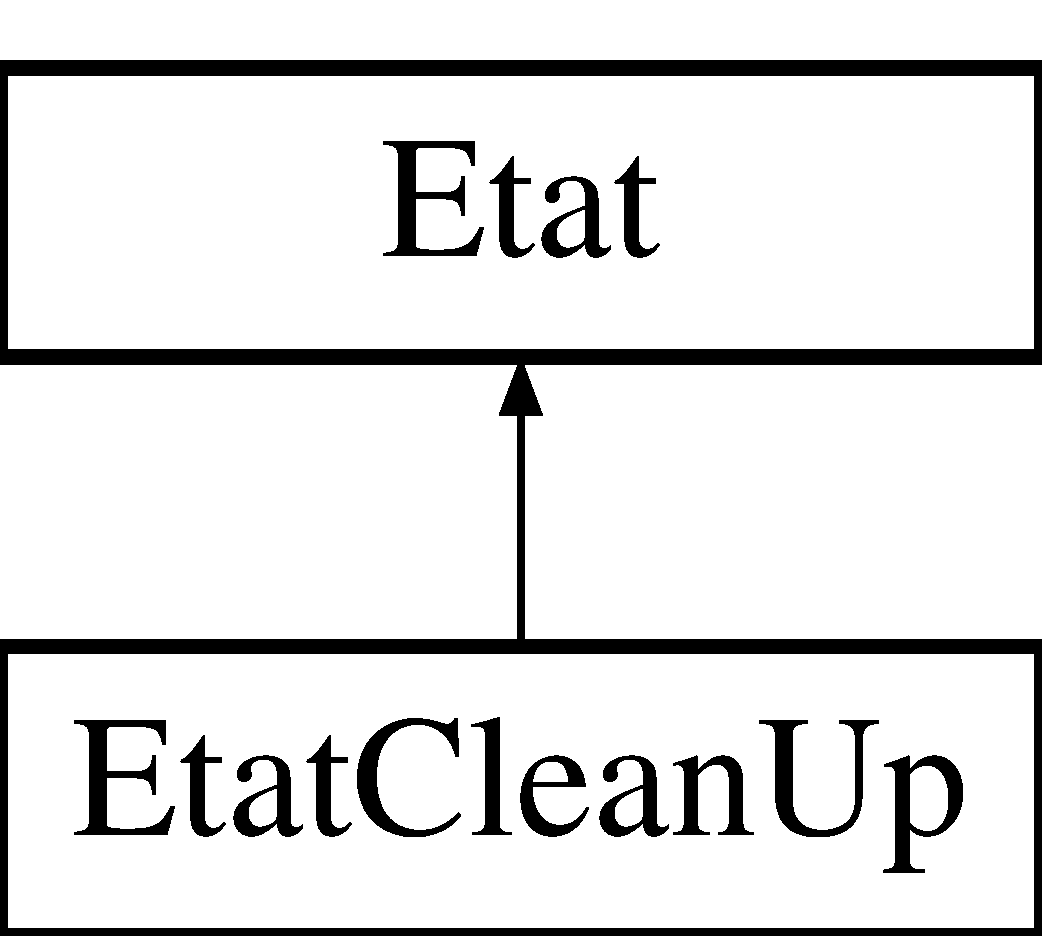
\includegraphics[height=2.000000cm]{class_etat_clean_up}
\end{center}
\end{figure}
\subsection*{Fonctions membres publiques}
\begin{DoxyCompactItemize}
\item 
\hyperlink{class_etat_clean_up_a04f3ac957a6a240981991bf170ef3d1a}{Etat\-Clean\-Up} (\hyperlink{class_jeu}{Jeu} $\ast$jeu)
\begin{DoxyCompactList}\small\item\em Constructeur. \end{DoxyCompactList}\item 
void \hyperlink{class_etat_clean_up_a58245fa6e240c4c4f20d1a1fca868571}{verification} ()
\begin{DoxyCompactList}\small\item\em \hyperlink{class_etat_clean_up}{Etat\-Clean\-Up} \-: procédè à toutes les vérification nécessaire et soit envoie vers \hyperlink{class_etat_fin}{Etat\-Fin}, soit prépare le jeu pour un nouveau tour et envoie vers \hyperlink{class_etat_pioche}{Etat\-Pioche}. \end{DoxyCompactList}\item 
void \hyperlink{class_etat_clean_up_aac0dacd1f4945a971ec72319c979a786}{Info\-Carte} ()
\begin{DoxyCompactList}\small\item\em \hyperlink{class_etat_clean_up}{Etat\-Clean\-Up} \-:aucun effet. \end{DoxyCompactList}\item 
void \hyperlink{class_etat_clean_up_a955f6fb5a4cffdbdca4348b90d59ad78}{retourner\-Carte} ()
\begin{DoxyCompactList}\small\item\em \hyperlink{class_etat_clean_up}{Etat\-Clean\-Up} \-:aucun effet. \end{DoxyCompactList}\item 
void \hyperlink{class_etat_clean_up_a3be20ce132ee978e5412ae54f36e4a78}{jouer\-Carte} ()
\begin{DoxyCompactList}\small\item\em \hyperlink{class_etat_clean_up}{Etat\-Clean\-Up} \-:aucun effet. \end{DoxyCompactList}\item 
void \hyperlink{class_etat_clean_up_a4c0dbb8c302a500052eccdc66c6a28b4}{confirmation} ()
\begin{DoxyCompactList}\small\item\em \hyperlink{class_etat_clean_up}{Etat\-Clean\-Up} \-:aucun effet. \end{DoxyCompactList}\item 
void \hyperlink{class_etat_clean_up_a7163c116050f238c7bcd43a7e9bae974}{annuler\-Action} ()
\begin{DoxyCompactList}\small\item\em \hyperlink{class_etat_clean_up}{Etat\-Clean\-Up} \-:aucun effet. \end{DoxyCompactList}\end{DoxyCompactItemize}


\subsection{Documentation des constructeurs et destructeur}
\hypertarget{class_etat_clean_up_a04f3ac957a6a240981991bf170ef3d1a}{\index{Etat\-Clean\-Up@{Etat\-Clean\-Up}!Etat\-Clean\-Up@{Etat\-Clean\-Up}}
\index{Etat\-Clean\-Up@{Etat\-Clean\-Up}!EtatCleanUp@{Etat\-Clean\-Up}}
\subsubsection[{Etat\-Clean\-Up}]{\setlength{\rightskip}{0pt plus 5cm}Etat\-Clean\-Up\-::\-Etat\-Clean\-Up (
\begin{DoxyParamCaption}
\item[{{\bf Jeu} $\ast$}]{jeu}
\end{DoxyParamCaption}
)\hspace{0.3cm}{\ttfamily [inline]}}}\label{class_etat_clean_up_a04f3ac957a6a240981991bf170ef3d1a}


Constructeur. 

Constructeur de la classe \hyperlink{class_etat_clean_up}{Etat\-Clean\-Up}


\begin{DoxyParams}{Paramètres}
{\em jeu} & \-: pointeur vers le jeu \\
\hline
\end{DoxyParams}


\subsection{Documentation des fonctions membres}
\hypertarget{class_etat_clean_up_a7163c116050f238c7bcd43a7e9bae974}{\index{Etat\-Clean\-Up@{Etat\-Clean\-Up}!annuler\-Action@{annuler\-Action}}
\index{annuler\-Action@{annuler\-Action}!EtatCleanUp@{Etat\-Clean\-Up}}
\subsubsection[{annuler\-Action}]{\setlength{\rightskip}{0pt plus 5cm}void Etat\-Clean\-Up\-::annuler\-Action (
\begin{DoxyParamCaption}
{}
\end{DoxyParamCaption}
)\hspace{0.3cm}{\ttfamily [virtual]}}}\label{class_etat_clean_up_a7163c116050f238c7bcd43a7e9bae974}


\hyperlink{class_etat_clean_up}{Etat\-Clean\-Up} \-:aucun effet. 



Implémente \hyperlink{class_etat_ac47332db984da58192bbb1c45f1702a8}{Etat}.

\hypertarget{class_etat_clean_up_a4c0dbb8c302a500052eccdc66c6a28b4}{\index{Etat\-Clean\-Up@{Etat\-Clean\-Up}!confirmation@{confirmation}}
\index{confirmation@{confirmation}!EtatCleanUp@{Etat\-Clean\-Up}}
\subsubsection[{confirmation}]{\setlength{\rightskip}{0pt plus 5cm}void Etat\-Clean\-Up\-::confirmation (
\begin{DoxyParamCaption}
{}
\end{DoxyParamCaption}
)\hspace{0.3cm}{\ttfamily [virtual]}}}\label{class_etat_clean_up_a4c0dbb8c302a500052eccdc66c6a28b4}


\hyperlink{class_etat_clean_up}{Etat\-Clean\-Up} \-:aucun effet. 



Implémente \hyperlink{class_etat_a65c2e505cda8cac2989b3a0c17a70278}{Etat}.

\hypertarget{class_etat_clean_up_aac0dacd1f4945a971ec72319c979a786}{\index{Etat\-Clean\-Up@{Etat\-Clean\-Up}!Info\-Carte@{Info\-Carte}}
\index{Info\-Carte@{Info\-Carte}!EtatCleanUp@{Etat\-Clean\-Up}}
\subsubsection[{Info\-Carte}]{\setlength{\rightskip}{0pt plus 5cm}void Etat\-Clean\-Up\-::\-Info\-Carte (
\begin{DoxyParamCaption}
{}
\end{DoxyParamCaption}
)\hspace{0.3cm}{\ttfamily [virtual]}}}\label{class_etat_clean_up_aac0dacd1f4945a971ec72319c979a786}


\hyperlink{class_etat_clean_up}{Etat\-Clean\-Up} \-:aucun effet. 



Implémente \hyperlink{class_etat_afd99ba60265bc0a82029d5fa2368acfa}{Etat}.

\hypertarget{class_etat_clean_up_a3be20ce132ee978e5412ae54f36e4a78}{\index{Etat\-Clean\-Up@{Etat\-Clean\-Up}!jouer\-Carte@{jouer\-Carte}}
\index{jouer\-Carte@{jouer\-Carte}!EtatCleanUp@{Etat\-Clean\-Up}}
\subsubsection[{jouer\-Carte}]{\setlength{\rightskip}{0pt plus 5cm}void Etat\-Clean\-Up\-::jouer\-Carte (
\begin{DoxyParamCaption}
{}
\end{DoxyParamCaption}
)\hspace{0.3cm}{\ttfamily [virtual]}}}\label{class_etat_clean_up_a3be20ce132ee978e5412ae54f36e4a78}


\hyperlink{class_etat_clean_up}{Etat\-Clean\-Up} \-:aucun effet. 



Implémente \hyperlink{class_etat_aaeffe08c27b2b64560726f5df95e6f3a}{Etat}.

\hypertarget{class_etat_clean_up_a955f6fb5a4cffdbdca4348b90d59ad78}{\index{Etat\-Clean\-Up@{Etat\-Clean\-Up}!retourner\-Carte@{retourner\-Carte}}
\index{retourner\-Carte@{retourner\-Carte}!EtatCleanUp@{Etat\-Clean\-Up}}
\subsubsection[{retourner\-Carte}]{\setlength{\rightskip}{0pt plus 5cm}void Etat\-Clean\-Up\-::retourner\-Carte (
\begin{DoxyParamCaption}
{}
\end{DoxyParamCaption}
)\hspace{0.3cm}{\ttfamily [virtual]}}}\label{class_etat_clean_up_a955f6fb5a4cffdbdca4348b90d59ad78}


\hyperlink{class_etat_clean_up}{Etat\-Clean\-Up} \-:aucun effet. 



Implémente \hyperlink{class_etat_a3d2fe662ffd20147763a25c4e06b56e9}{Etat}.

\hypertarget{class_etat_clean_up_a58245fa6e240c4c4f20d1a1fca868571}{\index{Etat\-Clean\-Up@{Etat\-Clean\-Up}!verification@{verification}}
\index{verification@{verification}!EtatCleanUp@{Etat\-Clean\-Up}}
\subsubsection[{verification}]{\setlength{\rightskip}{0pt plus 5cm}void Etat\-Clean\-Up\-::verification (
\begin{DoxyParamCaption}
{}
\end{DoxyParamCaption}
)\hspace{0.3cm}{\ttfamily [virtual]}}}\label{class_etat_clean_up_a58245fa6e240c4c4f20d1a1fca868571}


\hyperlink{class_etat_clean_up}{Etat\-Clean\-Up} \-: procédè à toutes les vérification nécessaire et soit envoie vers \hyperlink{class_etat_fin}{Etat\-Fin}, soit prépare le jeu pour un nouveau tour et envoie vers \hyperlink{class_etat_pioche}{Etat\-Pioche}. 



Implémente \hyperlink{class_etat_aaf949c7b45217b76ff68414e61ef0d2a}{Etat}.



La documentation de cette classe a été générée à partir du fichier suivant \-:\begin{DoxyCompactItemize}
\item 
/home/figiel-\/paul/\-Bureau/\-Projet\-Poo/\-Projet\-P\-O\-O-\/\-A\-R\-A\-Y\-A-\/\-F\-I\-G\-I\-E\-L/include/\hyperlink{_etat_clean_up_8hpp}{Etat\-Clean\-Up.\-hpp}\end{DoxyCompactItemize}

\hypertarget{class_etat_combo}{\section{Référence de la classe Etat\-Combo}
\label{class_etat_combo}\index{Etat\-Combo@{Etat\-Combo}}
}


{\ttfamily \#include $<$Etat\-Combo.\-hpp$>$}

Graphe d'héritage de Etat\-Combo\-:\begin{figure}[H]
\begin{center}
\leavevmode
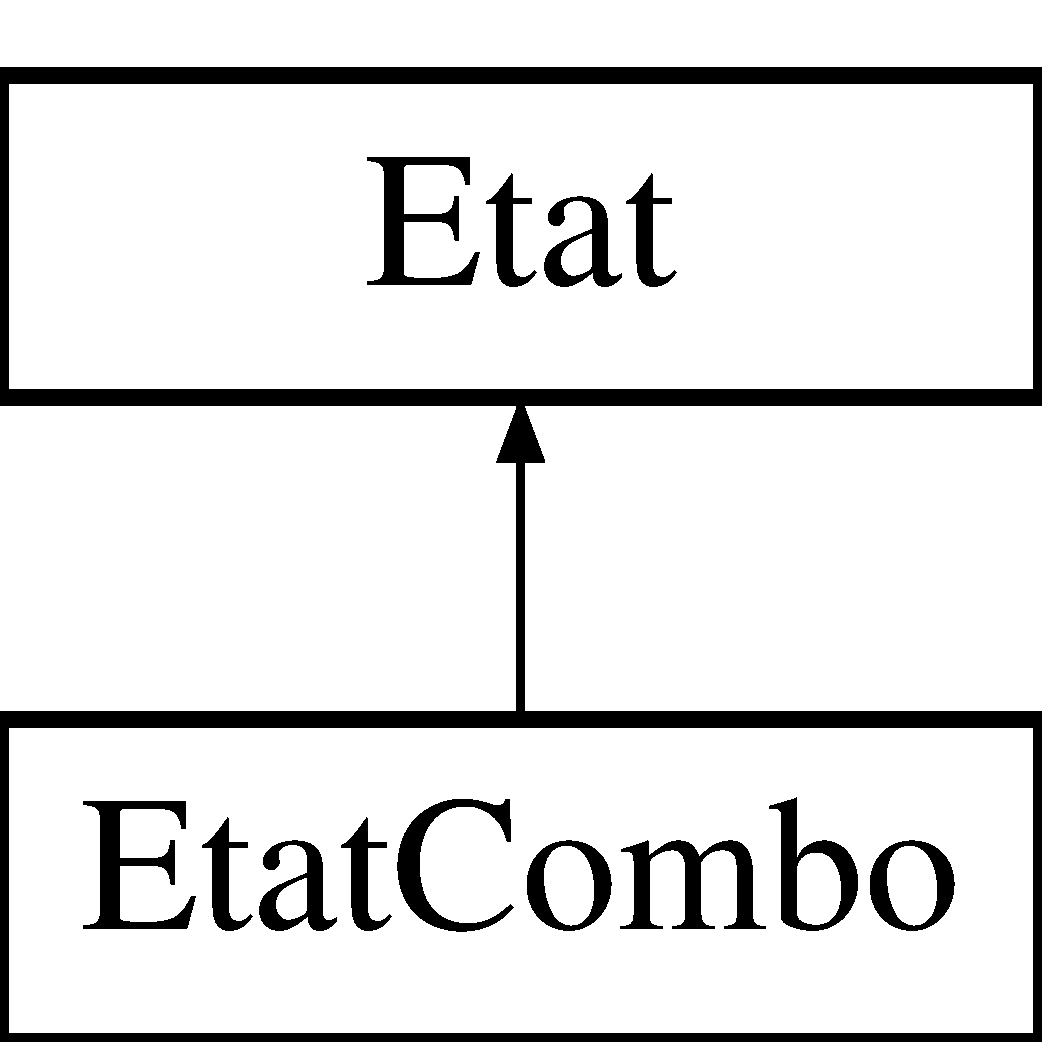
\includegraphics[height=2.000000cm]{class_etat_combo}
\end{center}
\end{figure}
\subsection*{Fonctions membres publiques}
\begin{DoxyCompactItemize}
\item 
\hyperlink{class_etat_combo_a182fe8d470e0851c869e4407c04f0e01}{Etat\-Combo} (\hyperlink{class_jeu}{Jeu} $\ast$jeu)
\begin{DoxyCompactList}\small\item\em Constructeur. \end{DoxyCompactList}\item 
void \hyperlink{class_etat_combo_a0a299d7c93ef09787eb0a402708475f0}{verification} ()
\begin{DoxyCompactList}\small\item\em \hyperlink{class_etat_combo}{Etat\-Combo} \-: aplique les effets de la carte jouer. \end{DoxyCompactList}\item 
void \hyperlink{class_etat_combo_a56b4cbe699ca50fc0e6ad4695a744bdf}{Info\-Carte} ()
\begin{DoxyCompactList}\small\item\em \hyperlink{class_etat_combo}{Etat\-Combo} \-: demande un numéro et affiche les infos de la carte corespondante de la main du joueur qui combo. \end{DoxyCompactList}\item 
void \hyperlink{class_etat_combo_a79944dfd6e471b633ad99cd2f3b70b02}{retourner\-Carte} ()
\begin{DoxyCompactList}\small\item\em \hyperlink{class_etat_combo}{Etat\-Combo} \-: demande un numéro et retourne la carte corespondante de la main du joueur qui combo. \end{DoxyCompactList}\item 
void \hyperlink{class_etat_combo_a6d7b6c040664a4c41380aca95f05f42c}{jouer\-Carte} ()
\begin{DoxyCompactList}\small\item\em \hyperlink{class_etat_combo}{Etat\-Combo} \-: demande un numéro et joue la carte corespondante de la main du joueur qui combo.( demande confirmation) \end{DoxyCompactList}\item 
void \hyperlink{class_etat_combo_a26ed3a79035572c4471aab88377470c5}{confirmation} ()
\begin{DoxyCompactList}\small\item\em \hyperlink{class_etat_combo}{Etat\-Combo} \-: si le joueur décide de confirmer qu'il veut jouer la carte qu'il vient de posé appelle vérification et passe à \hyperlink{class_etat_calc_dmg}{Etat\-Calc\-Dmg} ou reste dans \hyperlink{class_etat_combo}{Etat\-Combo} selon les cas. \end{DoxyCompactList}\item 
void \hyperlink{class_etat_combo_a18e6acc9e6e6a9db9a217d9aa044d778}{annuler\-Action} ()
\begin{DoxyCompactList}\small\item\em \hyperlink{class_etat_combo}{Etat\-Combo} \-: si le joueur décide de confirmer qu'il ne veut pas jouer la carte qu'il vient de posé la renvoie dans sa main. \end{DoxyCompactList}\end{DoxyCompactItemize}


\subsection{Documentation des constructeurs et destructeur}
\hypertarget{class_etat_combo_a182fe8d470e0851c869e4407c04f0e01}{\index{Etat\-Combo@{Etat\-Combo}!Etat\-Combo@{Etat\-Combo}}
\index{Etat\-Combo@{Etat\-Combo}!EtatCombo@{Etat\-Combo}}
\subsubsection[{Etat\-Combo}]{\setlength{\rightskip}{0pt plus 5cm}Etat\-Combo\-::\-Etat\-Combo (
\begin{DoxyParamCaption}
\item[{{\bf Jeu} $\ast$}]{jeu}
\end{DoxyParamCaption}
)\hspace{0.3cm}{\ttfamily [inline]}}}\label{class_etat_combo_a182fe8d470e0851c869e4407c04f0e01}


Constructeur. 

Constructeur de la classe \hyperlink{class_etat_combo}{Etat\-Combo}


\begin{DoxyParams}{Paramètres}
{\em jeu} & \-: pointeur vers le jeu \\
\hline
\end{DoxyParams}


\subsection{Documentation des fonctions membres}
\hypertarget{class_etat_combo_a18e6acc9e6e6a9db9a217d9aa044d778}{\index{Etat\-Combo@{Etat\-Combo}!annuler\-Action@{annuler\-Action}}
\index{annuler\-Action@{annuler\-Action}!EtatCombo@{Etat\-Combo}}
\subsubsection[{annuler\-Action}]{\setlength{\rightskip}{0pt plus 5cm}void Etat\-Combo\-::annuler\-Action (
\begin{DoxyParamCaption}
{}
\end{DoxyParamCaption}
)\hspace{0.3cm}{\ttfamily [virtual]}}}\label{class_etat_combo_a18e6acc9e6e6a9db9a217d9aa044d778}


\hyperlink{class_etat_combo}{Etat\-Combo} \-: si le joueur décide de confirmer qu'il ne veut pas jouer la carte qu'il vient de posé la renvoie dans sa main. 



Implémente \hyperlink{class_etat_ac47332db984da58192bbb1c45f1702a8}{Etat}.

\hypertarget{class_etat_combo_a26ed3a79035572c4471aab88377470c5}{\index{Etat\-Combo@{Etat\-Combo}!confirmation@{confirmation}}
\index{confirmation@{confirmation}!EtatCombo@{Etat\-Combo}}
\subsubsection[{confirmation}]{\setlength{\rightskip}{0pt plus 5cm}void Etat\-Combo\-::confirmation (
\begin{DoxyParamCaption}
{}
\end{DoxyParamCaption}
)\hspace{0.3cm}{\ttfamily [virtual]}}}\label{class_etat_combo_a26ed3a79035572c4471aab88377470c5}


\hyperlink{class_etat_combo}{Etat\-Combo} \-: si le joueur décide de confirmer qu'il veut jouer la carte qu'il vient de posé appelle vérification et passe à \hyperlink{class_etat_calc_dmg}{Etat\-Calc\-Dmg} ou reste dans \hyperlink{class_etat_combo}{Etat\-Combo} selon les cas. 



Implémente \hyperlink{class_etat_a65c2e505cda8cac2989b3a0c17a70278}{Etat}.

\hypertarget{class_etat_combo_a56b4cbe699ca50fc0e6ad4695a744bdf}{\index{Etat\-Combo@{Etat\-Combo}!Info\-Carte@{Info\-Carte}}
\index{Info\-Carte@{Info\-Carte}!EtatCombo@{Etat\-Combo}}
\subsubsection[{Info\-Carte}]{\setlength{\rightskip}{0pt plus 5cm}void Etat\-Combo\-::\-Info\-Carte (
\begin{DoxyParamCaption}
{}
\end{DoxyParamCaption}
)\hspace{0.3cm}{\ttfamily [virtual]}}}\label{class_etat_combo_a56b4cbe699ca50fc0e6ad4695a744bdf}


\hyperlink{class_etat_combo}{Etat\-Combo} \-: demande un numéro et affiche les infos de la carte corespondante de la main du joueur qui combo. 



Implémente \hyperlink{class_etat_afd99ba60265bc0a82029d5fa2368acfa}{Etat}.

\hypertarget{class_etat_combo_a6d7b6c040664a4c41380aca95f05f42c}{\index{Etat\-Combo@{Etat\-Combo}!jouer\-Carte@{jouer\-Carte}}
\index{jouer\-Carte@{jouer\-Carte}!EtatCombo@{Etat\-Combo}}
\subsubsection[{jouer\-Carte}]{\setlength{\rightskip}{0pt plus 5cm}void Etat\-Combo\-::jouer\-Carte (
\begin{DoxyParamCaption}
{}
\end{DoxyParamCaption}
)\hspace{0.3cm}{\ttfamily [virtual]}}}\label{class_etat_combo_a6d7b6c040664a4c41380aca95f05f42c}


\hyperlink{class_etat_combo}{Etat\-Combo} \-: demande un numéro et joue la carte corespondante de la main du joueur qui combo.( demande confirmation) 



Implémente \hyperlink{class_etat_aaeffe08c27b2b64560726f5df95e6f3a}{Etat}.

\hypertarget{class_etat_combo_a79944dfd6e471b633ad99cd2f3b70b02}{\index{Etat\-Combo@{Etat\-Combo}!retourner\-Carte@{retourner\-Carte}}
\index{retourner\-Carte@{retourner\-Carte}!EtatCombo@{Etat\-Combo}}
\subsubsection[{retourner\-Carte}]{\setlength{\rightskip}{0pt plus 5cm}void Etat\-Combo\-::retourner\-Carte (
\begin{DoxyParamCaption}
{}
\end{DoxyParamCaption}
)\hspace{0.3cm}{\ttfamily [virtual]}}}\label{class_etat_combo_a79944dfd6e471b633ad99cd2f3b70b02}


\hyperlink{class_etat_combo}{Etat\-Combo} \-: demande un numéro et retourne la carte corespondante de la main du joueur qui combo. 



Implémente \hyperlink{class_etat_a3d2fe662ffd20147763a25c4e06b56e9}{Etat}.

\hypertarget{class_etat_combo_a0a299d7c93ef09787eb0a402708475f0}{\index{Etat\-Combo@{Etat\-Combo}!verification@{verification}}
\index{verification@{verification}!EtatCombo@{Etat\-Combo}}
\subsubsection[{verification}]{\setlength{\rightskip}{0pt plus 5cm}void Etat\-Combo\-::verification (
\begin{DoxyParamCaption}
{}
\end{DoxyParamCaption}
)\hspace{0.3cm}{\ttfamily [virtual]}}}\label{class_etat_combo_a0a299d7c93ef09787eb0a402708475f0}


\hyperlink{class_etat_combo}{Etat\-Combo} \-: aplique les effets de la carte jouer. 



Implémente \hyperlink{class_etat_aaf949c7b45217b76ff68414e61ef0d2a}{Etat}.



La documentation de cette classe a été générée à partir du fichier suivant \-:\begin{DoxyCompactItemize}
\item 
/home/figiel-\/paul/\-Bureau/\-Projet\-Poo/\-Projet\-P\-O\-O-\/\-A\-R\-A\-Y\-A-\/\-F\-I\-G\-I\-E\-L/include/\hyperlink{_etat_combo_8hpp}{Etat\-Combo.\-hpp}\end{DoxyCompactItemize}

\hypertarget{class_etat_fin}{\section{Référence de la classe Etat\-Fin}
\label{class_etat_fin}\index{Etat\-Fin@{Etat\-Fin}}
}


{\ttfamily \#include $<$Etat\-Fin.\-hpp$>$}

Graphe d'héritage de Etat\-Fin\-:\begin{figure}[H]
\begin{center}
\leavevmode
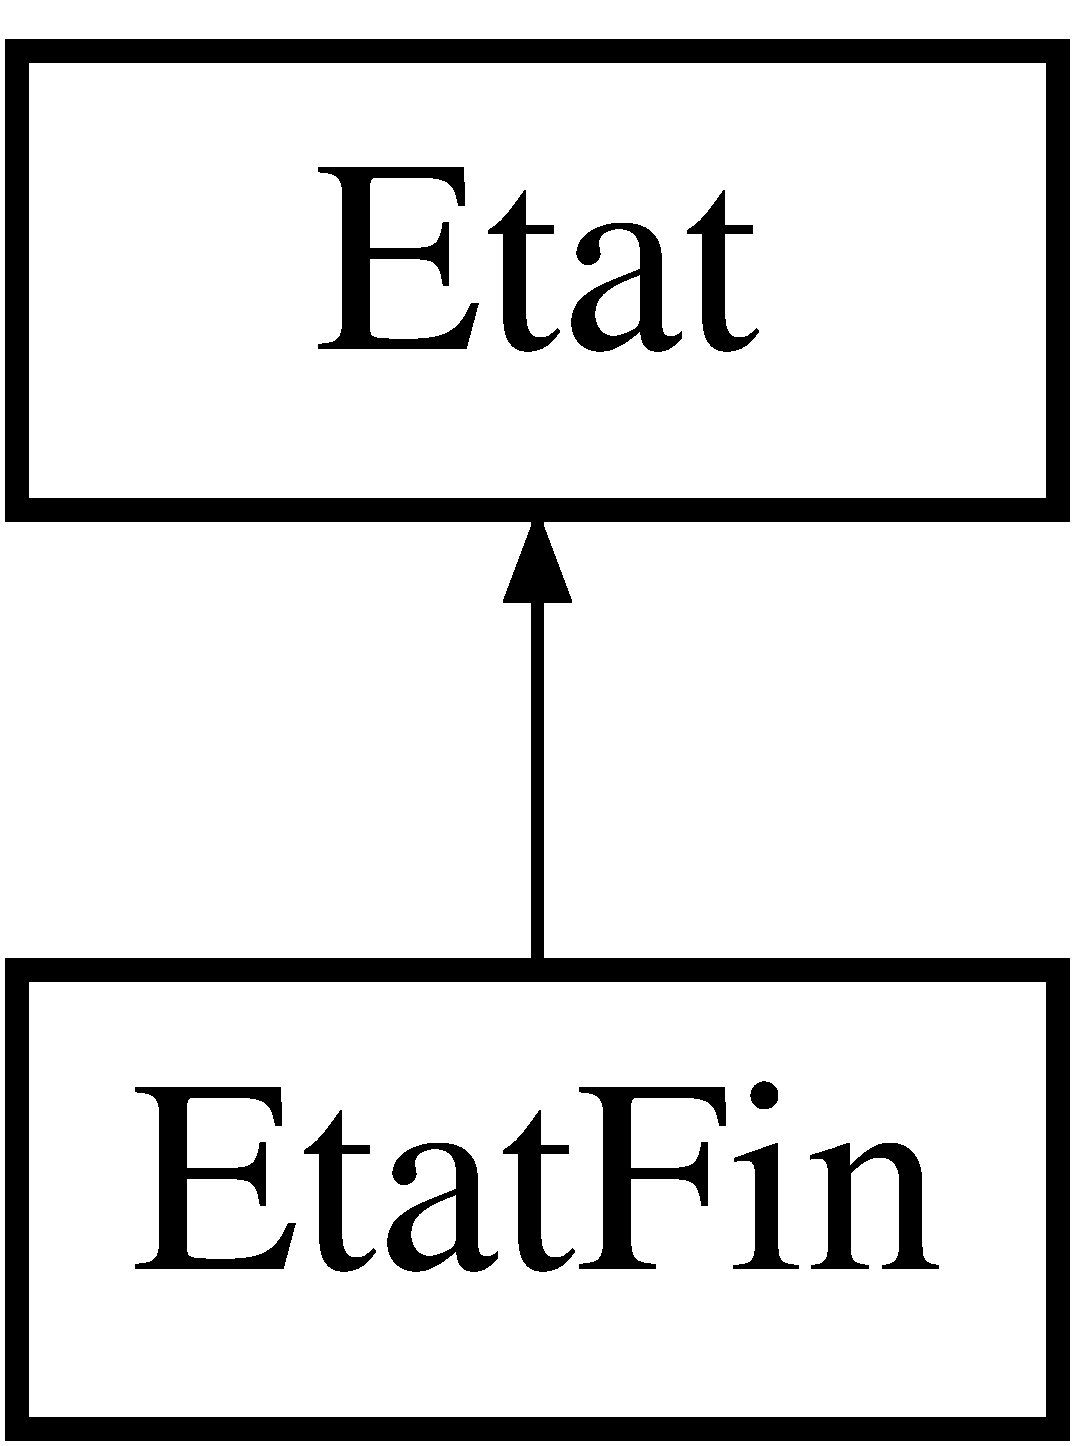
\includegraphics[height=2.000000cm]{class_etat_fin}
\end{center}
\end{figure}
\subsection*{Fonctions membres publiques}
\begin{DoxyCompactItemize}
\item 
\hyperlink{class_etat_fin_af6be08aa8a5e548075be8227d3b88523}{Etat\-Fin} (\hyperlink{class_jeu}{Jeu} $\ast$jeu)
\begin{DoxyCompactList}\small\item\em Constructeur. \end{DoxyCompactList}\item 
void \hyperlink{class_etat_fin_af5b612f37d0d38878b7380c7c44c8373}{verification} ()
\begin{DoxyCompactList}\small\item\em \hyperlink{class_etat_fin}{Etat\-Fin} \-: affiche le gagnant da la partie et fait que fini\-\_\- de classe jeu = true ( met fin à la partie) \end{DoxyCompactList}\item 
void \hyperlink{class_etat_fin_a60377a6cd48de413cb14445f8e9683bb}{Info\-Carte} ()
\begin{DoxyCompactList}\small\item\em \hyperlink{class_etat_fin}{Etat\-Fin} \-: aucun effet. \end{DoxyCompactList}\item 
void \hyperlink{class_etat_fin_a7772020d9101b4ebac666c498f023215}{retourner\-Carte} ()
\begin{DoxyCompactList}\small\item\em \hyperlink{class_etat_fin}{Etat\-Fin} \-: aucun effet. \end{DoxyCompactList}\item 
void \hyperlink{class_etat_fin_a8120a04c2f2e3632683a79a6b2fd524a}{jouer\-Carte} ()
\begin{DoxyCompactList}\small\item\em \hyperlink{class_etat_fin}{Etat\-Fin} \-: aucun effet. \end{DoxyCompactList}\item 
void \hyperlink{class_etat_fin_a218360ae56a421d500329f53c893822e}{confirmation} ()
\begin{DoxyCompactList}\small\item\em \hyperlink{class_etat_fin}{Etat\-Fin} \-: aucun effet. \end{DoxyCompactList}\item 
void \hyperlink{class_etat_fin_aa1ec559bd55dce76286b32b4cb293857}{annuler\-Action} ()
\begin{DoxyCompactList}\small\item\em \hyperlink{class_etat_fin}{Etat\-Fin} \-: aucun effet. \end{DoxyCompactList}\end{DoxyCompactItemize}


\subsection{Documentation des constructeurs et destructeur}
\hypertarget{class_etat_fin_af6be08aa8a5e548075be8227d3b88523}{\index{Etat\-Fin@{Etat\-Fin}!Etat\-Fin@{Etat\-Fin}}
\index{Etat\-Fin@{Etat\-Fin}!EtatFin@{Etat\-Fin}}
\subsubsection[{Etat\-Fin}]{\setlength{\rightskip}{0pt plus 5cm}Etat\-Fin\-::\-Etat\-Fin (
\begin{DoxyParamCaption}
\item[{{\bf Jeu} $\ast$}]{jeu}
\end{DoxyParamCaption}
)\hspace{0.3cm}{\ttfamily [inline]}}}\label{class_etat_fin_af6be08aa8a5e548075be8227d3b88523}


Constructeur. 

Constructeur de la classe \hyperlink{class_etat_fin}{Etat\-Fin}


\begin{DoxyParams}{Paramètres}
{\em jeu} & \-: pointeur vers le jeu \\
\hline
\end{DoxyParams}


\subsection{Documentation des fonctions membres}
\hypertarget{class_etat_fin_aa1ec559bd55dce76286b32b4cb293857}{\index{Etat\-Fin@{Etat\-Fin}!annuler\-Action@{annuler\-Action}}
\index{annuler\-Action@{annuler\-Action}!EtatFin@{Etat\-Fin}}
\subsubsection[{annuler\-Action}]{\setlength{\rightskip}{0pt plus 5cm}void Etat\-Fin\-::annuler\-Action (
\begin{DoxyParamCaption}
{}
\end{DoxyParamCaption}
)\hspace{0.3cm}{\ttfamily [virtual]}}}\label{class_etat_fin_aa1ec559bd55dce76286b32b4cb293857}


\hyperlink{class_etat_fin}{Etat\-Fin} \-: aucun effet. 



Implémente \hyperlink{class_etat_ac47332db984da58192bbb1c45f1702a8}{Etat}.

\hypertarget{class_etat_fin_a218360ae56a421d500329f53c893822e}{\index{Etat\-Fin@{Etat\-Fin}!confirmation@{confirmation}}
\index{confirmation@{confirmation}!EtatFin@{Etat\-Fin}}
\subsubsection[{confirmation}]{\setlength{\rightskip}{0pt plus 5cm}void Etat\-Fin\-::confirmation (
\begin{DoxyParamCaption}
{}
\end{DoxyParamCaption}
)\hspace{0.3cm}{\ttfamily [virtual]}}}\label{class_etat_fin_a218360ae56a421d500329f53c893822e}


\hyperlink{class_etat_fin}{Etat\-Fin} \-: aucun effet. 



Implémente \hyperlink{class_etat_a65c2e505cda8cac2989b3a0c17a70278}{Etat}.

\hypertarget{class_etat_fin_a60377a6cd48de413cb14445f8e9683bb}{\index{Etat\-Fin@{Etat\-Fin}!Info\-Carte@{Info\-Carte}}
\index{Info\-Carte@{Info\-Carte}!EtatFin@{Etat\-Fin}}
\subsubsection[{Info\-Carte}]{\setlength{\rightskip}{0pt plus 5cm}void Etat\-Fin\-::\-Info\-Carte (
\begin{DoxyParamCaption}
{}
\end{DoxyParamCaption}
)\hspace{0.3cm}{\ttfamily [virtual]}}}\label{class_etat_fin_a60377a6cd48de413cb14445f8e9683bb}


\hyperlink{class_etat_fin}{Etat\-Fin} \-: aucun effet. 



Implémente \hyperlink{class_etat_afd99ba60265bc0a82029d5fa2368acfa}{Etat}.

\hypertarget{class_etat_fin_a8120a04c2f2e3632683a79a6b2fd524a}{\index{Etat\-Fin@{Etat\-Fin}!jouer\-Carte@{jouer\-Carte}}
\index{jouer\-Carte@{jouer\-Carte}!EtatFin@{Etat\-Fin}}
\subsubsection[{jouer\-Carte}]{\setlength{\rightskip}{0pt plus 5cm}void Etat\-Fin\-::jouer\-Carte (
\begin{DoxyParamCaption}
{}
\end{DoxyParamCaption}
)\hspace{0.3cm}{\ttfamily [virtual]}}}\label{class_etat_fin_a8120a04c2f2e3632683a79a6b2fd524a}


\hyperlink{class_etat_fin}{Etat\-Fin} \-: aucun effet. 



Implémente \hyperlink{class_etat_aaeffe08c27b2b64560726f5df95e6f3a}{Etat}.

\hypertarget{class_etat_fin_a7772020d9101b4ebac666c498f023215}{\index{Etat\-Fin@{Etat\-Fin}!retourner\-Carte@{retourner\-Carte}}
\index{retourner\-Carte@{retourner\-Carte}!EtatFin@{Etat\-Fin}}
\subsubsection[{retourner\-Carte}]{\setlength{\rightskip}{0pt plus 5cm}void Etat\-Fin\-::retourner\-Carte (
\begin{DoxyParamCaption}
{}
\end{DoxyParamCaption}
)\hspace{0.3cm}{\ttfamily [virtual]}}}\label{class_etat_fin_a7772020d9101b4ebac666c498f023215}


\hyperlink{class_etat_fin}{Etat\-Fin} \-: aucun effet. 



Implémente \hyperlink{class_etat_a3d2fe662ffd20147763a25c4e06b56e9}{Etat}.

\hypertarget{class_etat_fin_af5b612f37d0d38878b7380c7c44c8373}{\index{Etat\-Fin@{Etat\-Fin}!verification@{verification}}
\index{verification@{verification}!EtatFin@{Etat\-Fin}}
\subsubsection[{verification}]{\setlength{\rightskip}{0pt plus 5cm}void Etat\-Fin\-::verification (
\begin{DoxyParamCaption}
{}
\end{DoxyParamCaption}
)\hspace{0.3cm}{\ttfamily [virtual]}}}\label{class_etat_fin_af5b612f37d0d38878b7380c7c44c8373}


\hyperlink{class_etat_fin}{Etat\-Fin} \-: affiche le gagnant da la partie et fait que fini\-\_\- de classe jeu = true ( met fin à la partie) 



Implémente \hyperlink{class_etat_aaf949c7b45217b76ff68414e61ef0d2a}{Etat}.



La documentation de cette classe a été générée à partir du fichier suivant \-:\begin{DoxyCompactItemize}
\item 
/home/figiel-\/paul/\-Bureau/\-Projet\-Poo/\-Projet\-P\-O\-O-\/\-A\-R\-A\-Y\-A-\/\-F\-I\-G\-I\-E\-L/include/\hyperlink{_etat_fin_8hpp}{Etat\-Fin.\-hpp}\end{DoxyCompactItemize}

\hypertarget{class_etat_pioche}{\section{Référence de la classe Etat\-Pioche}
\label{class_etat_pioche}\index{Etat\-Pioche@{Etat\-Pioche}}
}


{\ttfamily \#include $<$Etat\-Pioche.\-hpp$>$}

Graphe d'héritage de Etat\-Pioche\-:\begin{figure}[H]
\begin{center}
\leavevmode
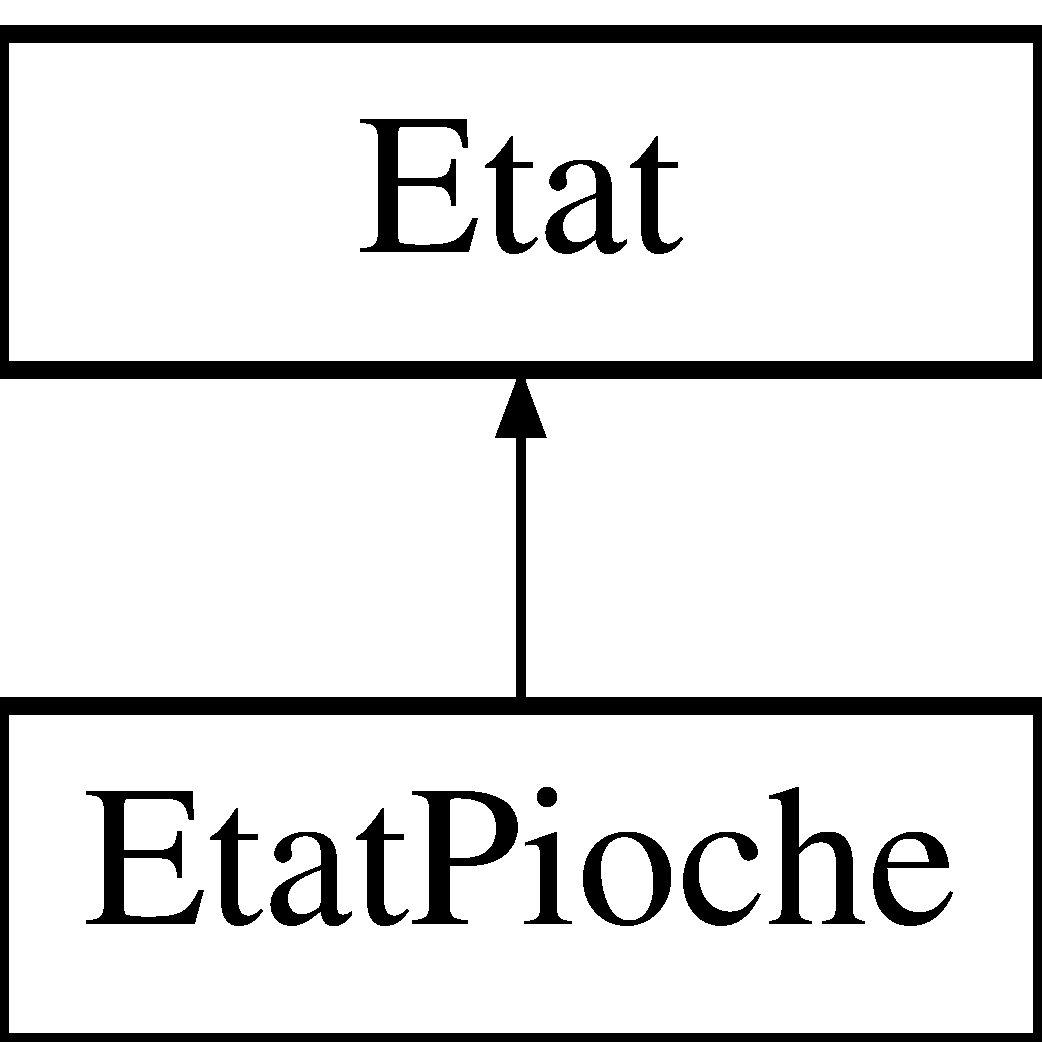
\includegraphics[height=2.000000cm]{class_etat_pioche}
\end{center}
\end{figure}
\subsection*{Fonctions membres publiques}
\begin{DoxyCompactItemize}
\item 
\hyperlink{class_etat_pioche_a7128040b6e05886001252c439eb65c20}{Etat\-Pioche} (\hyperlink{class_jeu}{Jeu} $\ast$jeu)
\begin{DoxyCompactList}\small\item\em Constructeur. \end{DoxyCompactList}\item 
void \hyperlink{class_etat_pioche_af429306bdc936b19982b604a686a230d}{verification} ()
\begin{DoxyCompactList}\small\item\em \hyperlink{class_etat_pioche}{Etat\-Pioche} \-: Fait piocher les 2 joueurs et aplique les effets des deux champion. \end{DoxyCompactList}\item 
void \hyperlink{class_etat_pioche_aa4379e774a3cfa7f3ce7f6668363f04f}{Info\-Carte} ()
\begin{DoxyCompactList}\small\item\em \hyperlink{class_etat_pioche}{Etat\-Pioche} \-: aucun effet. \end{DoxyCompactList}\item 
void \hyperlink{class_etat_pioche_ab139c9695f98b2e45df5fdc8f494ea80}{retourner\-Carte} ()
\begin{DoxyCompactList}\small\item\em \hyperlink{class_etat_pioche}{Etat\-Pioche} \-: aucun effet. \end{DoxyCompactList}\item 
void \hyperlink{class_etat_pioche_a951f62c333a41232cb4c09738925e7db}{jouer\-Carte} ()
\begin{DoxyCompactList}\small\item\em \hyperlink{class_etat_pioche}{Etat\-Pioche} \-: aucun effet. \end{DoxyCompactList}\item 
void \hyperlink{class_etat_pioche_ab3394a63db70d706b48501969edc7880}{confirmation} ()
\begin{DoxyCompactList}\small\item\em \hyperlink{class_etat_pioche}{Etat\-Pioche} \-: aucun effet. \end{DoxyCompactList}\item 
void \hyperlink{class_etat_pioche_a5c22d5a85ff1d59eb5facecee39e960b}{annuler\-Action} ()
\begin{DoxyCompactList}\small\item\em \hyperlink{class_etat_pioche}{Etat\-Pioche} \-: aucun effet. \end{DoxyCompactList}\end{DoxyCompactItemize}


\subsection{Documentation des constructeurs et destructeur}
\hypertarget{class_etat_pioche_a7128040b6e05886001252c439eb65c20}{\index{Etat\-Pioche@{Etat\-Pioche}!Etat\-Pioche@{Etat\-Pioche}}
\index{Etat\-Pioche@{Etat\-Pioche}!EtatPioche@{Etat\-Pioche}}
\subsubsection[{Etat\-Pioche}]{\setlength{\rightskip}{0pt plus 5cm}Etat\-Pioche\-::\-Etat\-Pioche (
\begin{DoxyParamCaption}
\item[{{\bf Jeu} $\ast$}]{jeu}
\end{DoxyParamCaption}
)\hspace{0.3cm}{\ttfamily [inline]}}}\label{class_etat_pioche_a7128040b6e05886001252c439eb65c20}


Constructeur. 

Constructeur de la classe \hyperlink{class_etat_pioche}{Etat\-Pioche}


\begin{DoxyParams}{Paramètres}
{\em jeu} & \-: pointeur vers le jeu \\
\hline
\end{DoxyParams}


\subsection{Documentation des fonctions membres}
\hypertarget{class_etat_pioche_a5c22d5a85ff1d59eb5facecee39e960b}{\index{Etat\-Pioche@{Etat\-Pioche}!annuler\-Action@{annuler\-Action}}
\index{annuler\-Action@{annuler\-Action}!EtatPioche@{Etat\-Pioche}}
\subsubsection[{annuler\-Action}]{\setlength{\rightskip}{0pt plus 5cm}void Etat\-Pioche\-::annuler\-Action (
\begin{DoxyParamCaption}
{}
\end{DoxyParamCaption}
)\hspace{0.3cm}{\ttfamily [virtual]}}}\label{class_etat_pioche_a5c22d5a85ff1d59eb5facecee39e960b}


\hyperlink{class_etat_pioche}{Etat\-Pioche} \-: aucun effet. 



Implémente \hyperlink{class_etat_ac47332db984da58192bbb1c45f1702a8}{Etat}.

\hypertarget{class_etat_pioche_ab3394a63db70d706b48501969edc7880}{\index{Etat\-Pioche@{Etat\-Pioche}!confirmation@{confirmation}}
\index{confirmation@{confirmation}!EtatPioche@{Etat\-Pioche}}
\subsubsection[{confirmation}]{\setlength{\rightskip}{0pt plus 5cm}void Etat\-Pioche\-::confirmation (
\begin{DoxyParamCaption}
{}
\end{DoxyParamCaption}
)\hspace{0.3cm}{\ttfamily [virtual]}}}\label{class_etat_pioche_ab3394a63db70d706b48501969edc7880}


\hyperlink{class_etat_pioche}{Etat\-Pioche} \-: aucun effet. 



Implémente \hyperlink{class_etat_a65c2e505cda8cac2989b3a0c17a70278}{Etat}.

\hypertarget{class_etat_pioche_aa4379e774a3cfa7f3ce7f6668363f04f}{\index{Etat\-Pioche@{Etat\-Pioche}!Info\-Carte@{Info\-Carte}}
\index{Info\-Carte@{Info\-Carte}!EtatPioche@{Etat\-Pioche}}
\subsubsection[{Info\-Carte}]{\setlength{\rightskip}{0pt plus 5cm}void Etat\-Pioche\-::\-Info\-Carte (
\begin{DoxyParamCaption}
{}
\end{DoxyParamCaption}
)\hspace{0.3cm}{\ttfamily [virtual]}}}\label{class_etat_pioche_aa4379e774a3cfa7f3ce7f6668363f04f}


\hyperlink{class_etat_pioche}{Etat\-Pioche} \-: aucun effet. 



Implémente \hyperlink{class_etat_afd99ba60265bc0a82029d5fa2368acfa}{Etat}.

\hypertarget{class_etat_pioche_a951f62c333a41232cb4c09738925e7db}{\index{Etat\-Pioche@{Etat\-Pioche}!jouer\-Carte@{jouer\-Carte}}
\index{jouer\-Carte@{jouer\-Carte}!EtatPioche@{Etat\-Pioche}}
\subsubsection[{jouer\-Carte}]{\setlength{\rightskip}{0pt plus 5cm}void Etat\-Pioche\-::jouer\-Carte (
\begin{DoxyParamCaption}
{}
\end{DoxyParamCaption}
)\hspace{0.3cm}{\ttfamily [virtual]}}}\label{class_etat_pioche_a951f62c333a41232cb4c09738925e7db}


\hyperlink{class_etat_pioche}{Etat\-Pioche} \-: aucun effet. 



Implémente \hyperlink{class_etat_aaeffe08c27b2b64560726f5df95e6f3a}{Etat}.

\hypertarget{class_etat_pioche_ab139c9695f98b2e45df5fdc8f494ea80}{\index{Etat\-Pioche@{Etat\-Pioche}!retourner\-Carte@{retourner\-Carte}}
\index{retourner\-Carte@{retourner\-Carte}!EtatPioche@{Etat\-Pioche}}
\subsubsection[{retourner\-Carte}]{\setlength{\rightskip}{0pt plus 5cm}void Etat\-Pioche\-::retourner\-Carte (
\begin{DoxyParamCaption}
{}
\end{DoxyParamCaption}
)\hspace{0.3cm}{\ttfamily [virtual]}}}\label{class_etat_pioche_ab139c9695f98b2e45df5fdc8f494ea80}


\hyperlink{class_etat_pioche}{Etat\-Pioche} \-: aucun effet. 



Implémente \hyperlink{class_etat_a3d2fe662ffd20147763a25c4e06b56e9}{Etat}.

\hypertarget{class_etat_pioche_af429306bdc936b19982b604a686a230d}{\index{Etat\-Pioche@{Etat\-Pioche}!verification@{verification}}
\index{verification@{verification}!EtatPioche@{Etat\-Pioche}}
\subsubsection[{verification}]{\setlength{\rightskip}{0pt plus 5cm}void Etat\-Pioche\-::verification (
\begin{DoxyParamCaption}
{}
\end{DoxyParamCaption}
)\hspace{0.3cm}{\ttfamily [virtual]}}}\label{class_etat_pioche_af429306bdc936b19982b604a686a230d}


\hyperlink{class_etat_pioche}{Etat\-Pioche} \-: Fait piocher les 2 joueurs et aplique les effets des deux champion. 



Implémente \hyperlink{class_etat_aaf949c7b45217b76ff68414e61ef0d2a}{Etat}.



La documentation de cette classe a été générée à partir du fichier suivant \-:\begin{DoxyCompactItemize}
\item 
/home/figiel-\/paul/\-Bureau/\-Projet\-Poo/\-Projet\-P\-O\-O-\/\-A\-R\-A\-Y\-A-\/\-F\-I\-G\-I\-E\-L/include/\hyperlink{_etat_pioche_8hpp}{Etat\-Pioche.\-hpp}\end{DoxyCompactItemize}

\hypertarget{class_jeu}{\section{Référence de la classe Jeu}
\label{class_jeu}\index{Jeu@{Jeu}}
}


{\ttfamily \#include $<$Jeu.\-hpp$>$}

Graphe d'héritage de Jeu\-:\begin{figure}[H]
\begin{center}
\leavevmode
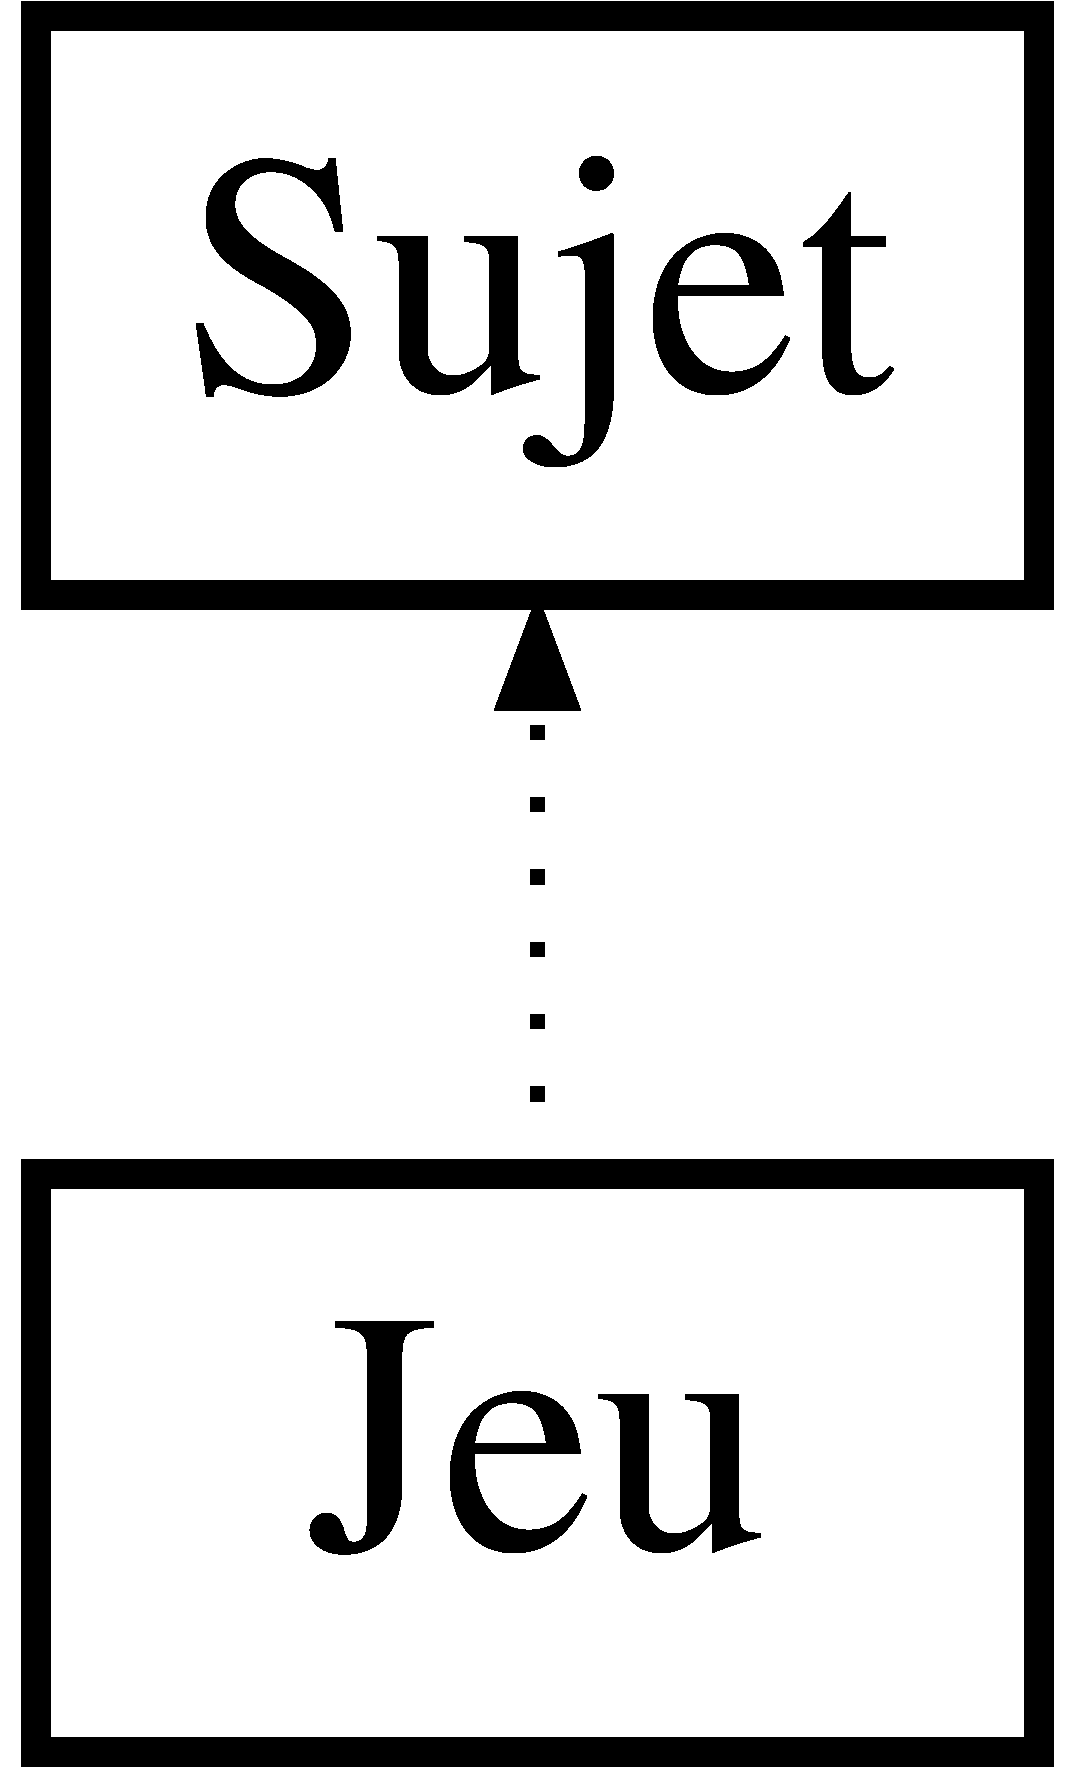
\includegraphics[height=2.000000cm]{class_jeu}
\end{center}
\end{figure}
\subsection*{Fonctions membres publiques}
\begin{DoxyCompactItemize}
\item 
\hyperlink{class_jeu_acc5795ee00edf75516d3dfe65be3e6d6}{Jeu} ()
\begin{DoxyCompactList}\small\item\em Constructeur. \end{DoxyCompactList}\item 
\hyperlink{class_joueur}{Joueur} $\ast$ \hyperlink{class_jeu_a56ed2a2cef42566e3c157cc11588e2ae}{get\-J1} ()
\item 
void \hyperlink{class_jeu_a74110004db819646a40323b1daa2c249}{set\-J1} (\hyperlink{class_joueur}{Joueur} $\ast$j)
\item 
\hyperlink{class_joueur}{Joueur} $\ast$ \hyperlink{class_jeu_afd1e01e7843d24cee637b41ffdfec9ad}{get\-J2} ()
\item 
void \hyperlink{class_jeu_a37c63b56c95a83753c6f9521e1d355b4}{set\-J2} (\hyperlink{class_joueur}{Joueur} $\ast$j)
\item 
std\-::vector$<$ \hyperlink{class_carte}{Carte} $\ast$ $>$ \hyperlink{class_jeu_ab6e4e2510694715b5a97fdeb73387cc6}{get\-Carte\-J1} ()
\item 
std\-::vector$<$ \hyperlink{class_carte}{Carte} $\ast$ $>$ \hyperlink{class_jeu_a86c6895722d29422a5bfe449ec2887f9}{get\-Carte\-J2} ()
\item 
std\-::vector$<$ \hyperlink{class_carte}{Carte} $\ast$ $>$ \hyperlink{class_jeu_ac4c93bb98ab4e39bfb6f433a68892c56}{get\-Rcarte\-J1} ()
\item 
std\-::vector$<$ \hyperlink{class_carte}{Carte} $\ast$ $>$ \hyperlink{class_jeu_ad1639e6ab51ce0704f20b4b389888e4a}{get\-Rcarte\-J2} ()
\item 
int \hyperlink{class_jeu_afded871bc0c3104ce1f0196ab4449663}{get\-Joue} ()
\item 
void \hyperlink{class_jeu_a3c7a41b6e9acc74ab8286adc0f6c99fc}{set\-Joue} (int x)
\item 
int \hyperlink{class_jeu_aedcf65c5f258409cd5539c7f3132b7b8}{get\-Gagnant\-Combat} ()
\item 
void \hyperlink{class_jeu_a02280609f3dc7843923f8de198d42654}{set\-Gagnant\-Combat} (int x)
\item 
int \hyperlink{class_jeu_a1bc939a24ccb8035cab265d022e909e3}{get\-Combo} ()
\item 
void \hyperlink{class_jeu_a306805dc1c5101f60da1f47fbb6208a9}{set\-Combo} (int x)
\item 
int \hyperlink{class_jeu_a872cd7c640a9f400f9328d270df62949}{get\-Combo\-Type\-J1} ()
\item 
void \hyperlink{class_jeu_aaf27565623c1570e13daa67a65a999e9}{set\-Combo\-Type\-J1} (int x)
\item 
int \hyperlink{class_jeu_adb7a2e6e6bfe15ed1d720e884faca987}{get\-Combo\-Type\-J2} ()
\item 
void \hyperlink{class_jeu_a0d437ab069b7e94694fd3d567dd20e07}{set\-Combo\-Type\-J2} (int x)
\item 
\hyperlink{class_etat}{Etat} $\ast$ \hyperlink{class_jeu_a2f0816cea4f78387b7ec71aa5e1f1b14}{get\-Etat\-Courant} ()
\item 
void \hyperlink{class_jeu_afc4543470bc3a4f4dc84b0aad4295d2d}{set\-Etat\-Courant} (\hyperlink{class_etat}{Etat} $\ast$et)
\item 
\hyperlink{class_etat}{Etat} $\ast$ \hyperlink{class_jeu_ab70c1e2ede9fb55f99b433d650f05813}{get\-Etat\-Pioche} ()
\item 
\hyperlink{class_etat}{Etat} $\ast$ \hyperlink{class_jeu_aeaa2da8046a84766358d2c4422d093d1}{get\-Etat\-Choix\-J1} ()
\item 
\hyperlink{class_etat}{Etat} $\ast$ \hyperlink{class_jeu_a0e916d9f16d3e0eb073027e4d9d56ef0}{get\-Etat\-Choix\-J2} ()
\item 
\hyperlink{class_etat}{Etat} $\ast$ \hyperlink{class_jeu_afc4788d06bf24260783e70bce3455ca3}{get\-Etat\-Choix\-Win} ()
\item 
\hyperlink{class_etat}{Etat} $\ast$ \hyperlink{class_jeu_ae804c0bd49285e41a28299f41d5eaaba}{get\-Etat\-Calc\-Dmg} ()
\item 
\hyperlink{class_etat}{Etat} $\ast$ \hyperlink{class_jeu_a8f4efbf2847eafdd86cd178b8b17ba24}{get\-Etat\-Bluff} ()
\item 
\hyperlink{class_etat}{Etat} $\ast$ \hyperlink{class_jeu_a2d0de8666c9f02c0af9186ec7e51643e}{get\-Etat\-Combo} ()
\item 
\hyperlink{class_etat}{Etat} $\ast$ \hyperlink{class_jeu_aa9469a1ced32c683eae7bec567c170d3}{get\-Etat\-Clean\-Up} ()
\item 
\hyperlink{class_etat}{Etat} $\ast$ \hyperlink{class_jeu_a372dba23eee1d33eb24e8f2dc3c3b6f4}{get\-Etat\-Fin} ()
\item 
bool \hyperlink{class_jeu_a724b71e7405bf1f28142973e20902691}{get\-Fini} ()
\item 
void \hyperlink{class_jeu_a9f48a5d4b43894bc584972eadc7ec1a1}{set\-Fini} (bool f)
\item 
bool \hyperlink{class_jeu_af8a568254fd6935e8814f31580300f0e}{get\-Bluff} ()
\item 
void \hyperlink{class_jeu_ac3e1701f943f16436a15e423bd2c6e62}{set\-Bluff} (bool b)
\item 
void \hyperlink{class_jeu_aacd7585f3235e9e0da4bcbfc6eef5ba9}{add\-Carte\-J1} (\hyperlink{class_carte}{Carte} $\ast$c)
\begin{DoxyCompactList}\small\item\em ajoute une carte à la liste des carte de J1 \end{DoxyCompactList}\item 
void \hyperlink{class_jeu_ab723c1aa7efb0961d83a53862ebd5122}{add\-Carte\-J2} (\hyperlink{class_carte}{Carte} $\ast$c)
\begin{DoxyCompactList}\small\item\em ajoute une carte à la liste des carte de J2 \end{DoxyCompactList}\item 
void \hyperlink{class_jeu_a6e61d83c15d2bd2bb0068dc58c4248f0}{add\-Rcarte\-J1} (\hyperlink{class_carte}{Carte} $\ast$c)
\begin{DoxyCompactList}\small\item\em ajoute une carte à la liste des carte à retourner de J1 \end{DoxyCompactList}\item 
void \hyperlink{class_jeu_adae51a9577a485942e3d349fa43be0f4}{add\-Rcarte\-J2} (\hyperlink{class_carte}{Carte} $\ast$c)
\begin{DoxyCompactList}\small\item\em ajoute une carte à la liste des carte à retourner de J2 \end{DoxyCompactList}\item 
void \hyperlink{class_jeu_aa5e5d255f55ff79dc50a149840240219}{vidage} ()
\item 
void \hyperlink{class_jeu_abd1b3f4f3866299296c37d5def7bd509}{retourner\-To\-Main} (int i)
\begin{DoxyCompactList}\small\item\em Retourne la dérnière carte jouer par le joueur i. \end{DoxyCompactList}\item 
void \hyperlink{class_jeu_af710d22785038c25866e270821a0d164}{clear\-Carte\-J1} ()
\begin{DoxyCompactList}\small\item\em vide le vector$<$\-Carte$\ast$$>$ carte\-J1\-\_\- \end{DoxyCompactList}\item 
void \hyperlink{class_jeu_ae62fc97f873d2c033b0b647db617f8f4}{clear\-Carte\-J2} ()
\begin{DoxyCompactList}\small\item\em vide le vector$<$\-Carte$\ast$$>$ carte\-J2\-\_\- \end{DoxyCompactList}\item 
void \hyperlink{class_jeu_a890ea4e42ea493a8179fdfb94b6c2fac}{clear\-R\-Carte\-J1} ()
\begin{DoxyCompactList}\small\item\em vide le vector$<$\-Carte$\ast$$>$ Rcarte\-J1\-\_\- \end{DoxyCompactList}\item 
void \hyperlink{class_jeu_ad41dfbbdde90ba9579173af18ea2a670}{clear\-R\-Carte\-J2} ()
\begin{DoxyCompactList}\small\item\em vide le vector$<$\-Carte$\ast$$>$ Rcarte\-J2\-\_\- \end{DoxyCompactList}\item 
void \hyperlink{class_jeu_a5a74a90faa114fd22a09ed25b9fc8381}{plus\-Combo} ()
\begin{DoxyCompactList}\small\item\em augmente de un le compteur de combo ( combo\-\_\-) \end{DoxyCompactList}\item 
void \hyperlink{class_jeu_af3b060e950164595e1e75901c7c701ad}{action\-Effet} (int i)
\begin{DoxyCompactList}\small\item\em applique l'effet de la derière carte jouer par le joueur i \end{DoxyCompactList}\item 
\hyperlink{class_carte}{Carte} $\ast$ \hyperlink{class_jeu_a71d1539ad625597004b324e15fc9bf7f}{get\-Last\-Carte} (int j)
\begin{DoxyCompactList}\small\item\em retourne la dérnière carte jouer par le joueur i \end{DoxyCompactList}\item 
int \hyperlink{class_jeu_a2b0a504e0fc5a6e5a74f362ab26d9633}{get\-Good\-Combo\-Type} (int x)
\begin{DoxyCompactList}\small\item\em retourne le type de combo du joueur i \end{DoxyCompactList}\item 
void \hyperlink{class_jeu_aee83ada0589e3352ec854b12e1c6e265}{ajouter\-Obs} (\hyperlink{class_observeur}{Observeur} $\ast$o)
\begin{DoxyCompactList}\small\item\em ajoute un observeur à jeu \end{DoxyCompactList}\item 
void \hyperlink{class_jeu_adbb1ba10c900ec336d744dbfd5de7f8e}{supprimer\-Obs} (int i)
\begin{DoxyCompactList}\small\item\em suprime un observeur du jeu \end{DoxyCompactList}\item 
void \hyperlink{class_jeu_ad955ffee4ed18add167fa957386a9821}{notifier\-Obs} ()
\begin{DoxyCompactList}\small\item\em notifie les observeur de jeu \end{DoxyCompactList}\item 
void \hyperlink{class_jeu_a56770ec2fa7af1cd5dfe1f06ee8d291a}{notifier\-Obs} (\hyperlink{class_observeur}{Observeur} $\ast$o)
\begin{DoxyCompactList}\small\item\em ajoute un observeur de jeu \end{DoxyCompactList}\end{DoxyCompactItemize}


\subsection{Documentation des constructeurs et destructeur}
\hypertarget{class_jeu_acc5795ee00edf75516d3dfe65be3e6d6}{\index{Jeu@{Jeu}!Jeu@{Jeu}}
\index{Jeu@{Jeu}!Jeu@{Jeu}}
\subsubsection[{Jeu}]{\setlength{\rightskip}{0pt plus 5cm}Jeu\-::\-Jeu (
\begin{DoxyParamCaption}
{}
\end{DoxyParamCaption}
)}}\label{class_jeu_acc5795ee00edf75516d3dfe65be3e6d6}


Constructeur. 

les des observeurs

Constructeur de la classe \hyperlink{class_jeu}{Jeu} 

\subsection{Documentation des fonctions membres}
\hypertarget{class_jeu_af3b060e950164595e1e75901c7c701ad}{\index{Jeu@{Jeu}!action\-Effet@{action\-Effet}}
\index{action\-Effet@{action\-Effet}!Jeu@{Jeu}}
\subsubsection[{action\-Effet}]{\setlength{\rightskip}{0pt plus 5cm}void Jeu\-::action\-Effet (
\begin{DoxyParamCaption}
\item[{int}]{i}
\end{DoxyParamCaption}
)}}\label{class_jeu_af3b060e950164595e1e75901c7c701ad}


applique l'effet de la derière carte jouer par le joueur i 


\begin{DoxyParams}{Paramètres}
{\em int} & i \-: le joueur concerner \\
\hline
\end{DoxyParams}
\hypertarget{class_jeu_aacd7585f3235e9e0da4bcbfc6eef5ba9}{\index{Jeu@{Jeu}!add\-Carte\-J1@{add\-Carte\-J1}}
\index{add\-Carte\-J1@{add\-Carte\-J1}!Jeu@{Jeu}}
\subsubsection[{add\-Carte\-J1}]{\setlength{\rightskip}{0pt plus 5cm}void Jeu\-::add\-Carte\-J1 (
\begin{DoxyParamCaption}
\item[{{\bf Carte} $\ast$}]{c}
\end{DoxyParamCaption}
)}}\label{class_jeu_aacd7585f3235e9e0da4bcbfc6eef5ba9}


ajoute une carte à la liste des carte de J1 


\begin{DoxyParams}{Paramètres}
{\em Carte$\ast$} & c \-: carte à rajouter \\
\hline
\end{DoxyParams}
\hypertarget{class_jeu_ab723c1aa7efb0961d83a53862ebd5122}{\index{Jeu@{Jeu}!add\-Carte\-J2@{add\-Carte\-J2}}
\index{add\-Carte\-J2@{add\-Carte\-J2}!Jeu@{Jeu}}
\subsubsection[{add\-Carte\-J2}]{\setlength{\rightskip}{0pt plus 5cm}void Jeu\-::add\-Carte\-J2 (
\begin{DoxyParamCaption}
\item[{{\bf Carte} $\ast$}]{c}
\end{DoxyParamCaption}
)}}\label{class_jeu_ab723c1aa7efb0961d83a53862ebd5122}


ajoute une carte à la liste des carte de J2 


\begin{DoxyParams}{Paramètres}
{\em Carte$\ast$} & c \-: carte à rajouter \\
\hline
\end{DoxyParams}
\hypertarget{class_jeu_a6e61d83c15d2bd2bb0068dc58c4248f0}{\index{Jeu@{Jeu}!add\-Rcarte\-J1@{add\-Rcarte\-J1}}
\index{add\-Rcarte\-J1@{add\-Rcarte\-J1}!Jeu@{Jeu}}
\subsubsection[{add\-Rcarte\-J1}]{\setlength{\rightskip}{0pt plus 5cm}void Jeu\-::add\-Rcarte\-J1 (
\begin{DoxyParamCaption}
\item[{{\bf Carte} $\ast$}]{c}
\end{DoxyParamCaption}
)}}\label{class_jeu_a6e61d83c15d2bd2bb0068dc58c4248f0}


ajoute une carte à la liste des carte à retourner de J1 


\begin{DoxyParams}{Paramètres}
{\em Carte$\ast$} & c \-: carte à rajouter \\
\hline
\end{DoxyParams}
\hypertarget{class_jeu_adae51a9577a485942e3d349fa43be0f4}{\index{Jeu@{Jeu}!add\-Rcarte\-J2@{add\-Rcarte\-J2}}
\index{add\-Rcarte\-J2@{add\-Rcarte\-J2}!Jeu@{Jeu}}
\subsubsection[{add\-Rcarte\-J2}]{\setlength{\rightskip}{0pt plus 5cm}void Jeu\-::add\-Rcarte\-J2 (
\begin{DoxyParamCaption}
\item[{{\bf Carte} $\ast$}]{c}
\end{DoxyParamCaption}
)}}\label{class_jeu_adae51a9577a485942e3d349fa43be0f4}


ajoute une carte à la liste des carte à retourner de J2 


\begin{DoxyParams}{Paramètres}
{\em Carte$\ast$} & c \-: carte à rajouter \\
\hline
\end{DoxyParams}
\hypertarget{class_jeu_aee83ada0589e3352ec854b12e1c6e265}{\index{Jeu@{Jeu}!ajouter\-Obs@{ajouter\-Obs}}
\index{ajouter\-Obs@{ajouter\-Obs}!Jeu@{Jeu}}
\subsubsection[{ajouter\-Obs}]{\setlength{\rightskip}{0pt plus 5cm}void Jeu\-::ajouter\-Obs (
\begin{DoxyParamCaption}
\item[{{\bf Observeur} $\ast$}]{o}
\end{DoxyParamCaption}
)\hspace{0.3cm}{\ttfamily [virtual]}}}\label{class_jeu_aee83ada0589e3352ec854b12e1c6e265}


ajoute un observeur à jeu 


\begin{DoxyParams}{Paramètres}
{\em Oberserveur} & $\ast$o \-: l'observeur à rajouté \\
\hline
\end{DoxyParams}


Implémente \hyperlink{class_sujet_a77c41db2a06015ca931da1636e4dbc6d}{Sujet}.

\hypertarget{class_jeu_af710d22785038c25866e270821a0d164}{\index{Jeu@{Jeu}!clear\-Carte\-J1@{clear\-Carte\-J1}}
\index{clear\-Carte\-J1@{clear\-Carte\-J1}!Jeu@{Jeu}}
\subsubsection[{clear\-Carte\-J1}]{\setlength{\rightskip}{0pt plus 5cm}void Jeu\-::clear\-Carte\-J1 (
\begin{DoxyParamCaption}
{}
\end{DoxyParamCaption}
)}}\label{class_jeu_af710d22785038c25866e270821a0d164}


vide le vector$<$\-Carte$\ast$$>$ carte\-J1\-\_\- 

\hypertarget{class_jeu_ae62fc97f873d2c033b0b647db617f8f4}{\index{Jeu@{Jeu}!clear\-Carte\-J2@{clear\-Carte\-J2}}
\index{clear\-Carte\-J2@{clear\-Carte\-J2}!Jeu@{Jeu}}
\subsubsection[{clear\-Carte\-J2}]{\setlength{\rightskip}{0pt plus 5cm}void Jeu\-::clear\-Carte\-J2 (
\begin{DoxyParamCaption}
{}
\end{DoxyParamCaption}
)}}\label{class_jeu_ae62fc97f873d2c033b0b647db617f8f4}


vide le vector$<$\-Carte$\ast$$>$ carte\-J2\-\_\- 

\hypertarget{class_jeu_a890ea4e42ea493a8179fdfb94b6c2fac}{\index{Jeu@{Jeu}!clear\-R\-Carte\-J1@{clear\-R\-Carte\-J1}}
\index{clear\-R\-Carte\-J1@{clear\-R\-Carte\-J1}!Jeu@{Jeu}}
\subsubsection[{clear\-R\-Carte\-J1}]{\setlength{\rightskip}{0pt plus 5cm}void Jeu\-::clear\-R\-Carte\-J1 (
\begin{DoxyParamCaption}
{}
\end{DoxyParamCaption}
)}}\label{class_jeu_a890ea4e42ea493a8179fdfb94b6c2fac}


vide le vector$<$\-Carte$\ast$$>$ Rcarte\-J1\-\_\- 

\hypertarget{class_jeu_ad41dfbbdde90ba9579173af18ea2a670}{\index{Jeu@{Jeu}!clear\-R\-Carte\-J2@{clear\-R\-Carte\-J2}}
\index{clear\-R\-Carte\-J2@{clear\-R\-Carte\-J2}!Jeu@{Jeu}}
\subsubsection[{clear\-R\-Carte\-J2}]{\setlength{\rightskip}{0pt plus 5cm}void Jeu\-::clear\-R\-Carte\-J2 (
\begin{DoxyParamCaption}
{}
\end{DoxyParamCaption}
)}}\label{class_jeu_ad41dfbbdde90ba9579173af18ea2a670}


vide le vector$<$\-Carte$\ast$$>$ Rcarte\-J2\-\_\- 

\hypertarget{class_jeu_af8a568254fd6935e8814f31580300f0e}{\index{Jeu@{Jeu}!get\-Bluff@{get\-Bluff}}
\index{get\-Bluff@{get\-Bluff}!Jeu@{Jeu}}
\subsubsection[{get\-Bluff}]{\setlength{\rightskip}{0pt plus 5cm}bool Jeu\-::get\-Bluff (
\begin{DoxyParamCaption}
{}
\end{DoxyParamCaption}
)\hspace{0.3cm}{\ttfamily [inline]}}}\label{class_jeu_af8a568254fd6935e8814f31580300f0e}
\hypertarget{class_jeu_ab6e4e2510694715b5a97fdeb73387cc6}{\index{Jeu@{Jeu}!get\-Carte\-J1@{get\-Carte\-J1}}
\index{get\-Carte\-J1@{get\-Carte\-J1}!Jeu@{Jeu}}
\subsubsection[{get\-Carte\-J1}]{\setlength{\rightskip}{0pt plus 5cm}std\-::vector$<${\bf Carte}$\ast$$>$ Jeu\-::get\-Carte\-J1 (
\begin{DoxyParamCaption}
{}
\end{DoxyParamCaption}
)\hspace{0.3cm}{\ttfamily [inline]}}}\label{class_jeu_ab6e4e2510694715b5a97fdeb73387cc6}
\hypertarget{class_jeu_a86c6895722d29422a5bfe449ec2887f9}{\index{Jeu@{Jeu}!get\-Carte\-J2@{get\-Carte\-J2}}
\index{get\-Carte\-J2@{get\-Carte\-J2}!Jeu@{Jeu}}
\subsubsection[{get\-Carte\-J2}]{\setlength{\rightskip}{0pt plus 5cm}std\-::vector$<${\bf Carte}$\ast$$>$ Jeu\-::get\-Carte\-J2 (
\begin{DoxyParamCaption}
{}
\end{DoxyParamCaption}
)\hspace{0.3cm}{\ttfamily [inline]}}}\label{class_jeu_a86c6895722d29422a5bfe449ec2887f9}
\hypertarget{class_jeu_a1bc939a24ccb8035cab265d022e909e3}{\index{Jeu@{Jeu}!get\-Combo@{get\-Combo}}
\index{get\-Combo@{get\-Combo}!Jeu@{Jeu}}
\subsubsection[{get\-Combo}]{\setlength{\rightskip}{0pt plus 5cm}int Jeu\-::get\-Combo (
\begin{DoxyParamCaption}
{}
\end{DoxyParamCaption}
)\hspace{0.3cm}{\ttfamily [inline]}}}\label{class_jeu_a1bc939a24ccb8035cab265d022e909e3}
\hypertarget{class_jeu_a872cd7c640a9f400f9328d270df62949}{\index{Jeu@{Jeu}!get\-Combo\-Type\-J1@{get\-Combo\-Type\-J1}}
\index{get\-Combo\-Type\-J1@{get\-Combo\-Type\-J1}!Jeu@{Jeu}}
\subsubsection[{get\-Combo\-Type\-J1}]{\setlength{\rightskip}{0pt plus 5cm}int Jeu\-::get\-Combo\-Type\-J1 (
\begin{DoxyParamCaption}
{}
\end{DoxyParamCaption}
)\hspace{0.3cm}{\ttfamily [inline]}}}\label{class_jeu_a872cd7c640a9f400f9328d270df62949}
\hypertarget{class_jeu_adb7a2e6e6bfe15ed1d720e884faca987}{\index{Jeu@{Jeu}!get\-Combo\-Type\-J2@{get\-Combo\-Type\-J2}}
\index{get\-Combo\-Type\-J2@{get\-Combo\-Type\-J2}!Jeu@{Jeu}}
\subsubsection[{get\-Combo\-Type\-J2}]{\setlength{\rightskip}{0pt plus 5cm}int Jeu\-::get\-Combo\-Type\-J2 (
\begin{DoxyParamCaption}
{}
\end{DoxyParamCaption}
)\hspace{0.3cm}{\ttfamily [inline]}}}\label{class_jeu_adb7a2e6e6bfe15ed1d720e884faca987}
\hypertarget{class_jeu_a8f4efbf2847eafdd86cd178b8b17ba24}{\index{Jeu@{Jeu}!get\-Etat\-Bluff@{get\-Etat\-Bluff}}
\index{get\-Etat\-Bluff@{get\-Etat\-Bluff}!Jeu@{Jeu}}
\subsubsection[{get\-Etat\-Bluff}]{\setlength{\rightskip}{0pt plus 5cm}{\bf Etat}$\ast$ Jeu\-::get\-Etat\-Bluff (
\begin{DoxyParamCaption}
{}
\end{DoxyParamCaption}
)\hspace{0.3cm}{\ttfamily [inline]}}}\label{class_jeu_a8f4efbf2847eafdd86cd178b8b17ba24}
\hypertarget{class_jeu_ae804c0bd49285e41a28299f41d5eaaba}{\index{Jeu@{Jeu}!get\-Etat\-Calc\-Dmg@{get\-Etat\-Calc\-Dmg}}
\index{get\-Etat\-Calc\-Dmg@{get\-Etat\-Calc\-Dmg}!Jeu@{Jeu}}
\subsubsection[{get\-Etat\-Calc\-Dmg}]{\setlength{\rightskip}{0pt plus 5cm}{\bf Etat}$\ast$ Jeu\-::get\-Etat\-Calc\-Dmg (
\begin{DoxyParamCaption}
{}
\end{DoxyParamCaption}
)\hspace{0.3cm}{\ttfamily [inline]}}}\label{class_jeu_ae804c0bd49285e41a28299f41d5eaaba}
\hypertarget{class_jeu_aeaa2da8046a84766358d2c4422d093d1}{\index{Jeu@{Jeu}!get\-Etat\-Choix\-J1@{get\-Etat\-Choix\-J1}}
\index{get\-Etat\-Choix\-J1@{get\-Etat\-Choix\-J1}!Jeu@{Jeu}}
\subsubsection[{get\-Etat\-Choix\-J1}]{\setlength{\rightskip}{0pt plus 5cm}{\bf Etat}$\ast$ Jeu\-::get\-Etat\-Choix\-J1 (
\begin{DoxyParamCaption}
{}
\end{DoxyParamCaption}
)\hspace{0.3cm}{\ttfamily [inline]}}}\label{class_jeu_aeaa2da8046a84766358d2c4422d093d1}
\hypertarget{class_jeu_a0e916d9f16d3e0eb073027e4d9d56ef0}{\index{Jeu@{Jeu}!get\-Etat\-Choix\-J2@{get\-Etat\-Choix\-J2}}
\index{get\-Etat\-Choix\-J2@{get\-Etat\-Choix\-J2}!Jeu@{Jeu}}
\subsubsection[{get\-Etat\-Choix\-J2}]{\setlength{\rightskip}{0pt plus 5cm}{\bf Etat}$\ast$ Jeu\-::get\-Etat\-Choix\-J2 (
\begin{DoxyParamCaption}
{}
\end{DoxyParamCaption}
)\hspace{0.3cm}{\ttfamily [inline]}}}\label{class_jeu_a0e916d9f16d3e0eb073027e4d9d56ef0}
\hypertarget{class_jeu_afc4788d06bf24260783e70bce3455ca3}{\index{Jeu@{Jeu}!get\-Etat\-Choix\-Win@{get\-Etat\-Choix\-Win}}
\index{get\-Etat\-Choix\-Win@{get\-Etat\-Choix\-Win}!Jeu@{Jeu}}
\subsubsection[{get\-Etat\-Choix\-Win}]{\setlength{\rightskip}{0pt plus 5cm}{\bf Etat}$\ast$ Jeu\-::get\-Etat\-Choix\-Win (
\begin{DoxyParamCaption}
{}
\end{DoxyParamCaption}
)\hspace{0.3cm}{\ttfamily [inline]}}}\label{class_jeu_afc4788d06bf24260783e70bce3455ca3}
\hypertarget{class_jeu_aa9469a1ced32c683eae7bec567c170d3}{\index{Jeu@{Jeu}!get\-Etat\-Clean\-Up@{get\-Etat\-Clean\-Up}}
\index{get\-Etat\-Clean\-Up@{get\-Etat\-Clean\-Up}!Jeu@{Jeu}}
\subsubsection[{get\-Etat\-Clean\-Up}]{\setlength{\rightskip}{0pt plus 5cm}{\bf Etat}$\ast$ Jeu\-::get\-Etat\-Clean\-Up (
\begin{DoxyParamCaption}
{}
\end{DoxyParamCaption}
)\hspace{0.3cm}{\ttfamily [inline]}}}\label{class_jeu_aa9469a1ced32c683eae7bec567c170d3}
\hypertarget{class_jeu_a2d0de8666c9f02c0af9186ec7e51643e}{\index{Jeu@{Jeu}!get\-Etat\-Combo@{get\-Etat\-Combo}}
\index{get\-Etat\-Combo@{get\-Etat\-Combo}!Jeu@{Jeu}}
\subsubsection[{get\-Etat\-Combo}]{\setlength{\rightskip}{0pt plus 5cm}{\bf Etat}$\ast$ Jeu\-::get\-Etat\-Combo (
\begin{DoxyParamCaption}
{}
\end{DoxyParamCaption}
)\hspace{0.3cm}{\ttfamily [inline]}}}\label{class_jeu_a2d0de8666c9f02c0af9186ec7e51643e}
\hypertarget{class_jeu_a2f0816cea4f78387b7ec71aa5e1f1b14}{\index{Jeu@{Jeu}!get\-Etat\-Courant@{get\-Etat\-Courant}}
\index{get\-Etat\-Courant@{get\-Etat\-Courant}!Jeu@{Jeu}}
\subsubsection[{get\-Etat\-Courant}]{\setlength{\rightskip}{0pt plus 5cm}{\bf Etat}$\ast$ Jeu\-::get\-Etat\-Courant (
\begin{DoxyParamCaption}
{}
\end{DoxyParamCaption}
)\hspace{0.3cm}{\ttfamily [inline]}}}\label{class_jeu_a2f0816cea4f78387b7ec71aa5e1f1b14}
\hypertarget{class_jeu_a372dba23eee1d33eb24e8f2dc3c3b6f4}{\index{Jeu@{Jeu}!get\-Etat\-Fin@{get\-Etat\-Fin}}
\index{get\-Etat\-Fin@{get\-Etat\-Fin}!Jeu@{Jeu}}
\subsubsection[{get\-Etat\-Fin}]{\setlength{\rightskip}{0pt plus 5cm}{\bf Etat}$\ast$ Jeu\-::get\-Etat\-Fin (
\begin{DoxyParamCaption}
{}
\end{DoxyParamCaption}
)\hspace{0.3cm}{\ttfamily [inline]}}}\label{class_jeu_a372dba23eee1d33eb24e8f2dc3c3b6f4}
\hypertarget{class_jeu_ab70c1e2ede9fb55f99b433d650f05813}{\index{Jeu@{Jeu}!get\-Etat\-Pioche@{get\-Etat\-Pioche}}
\index{get\-Etat\-Pioche@{get\-Etat\-Pioche}!Jeu@{Jeu}}
\subsubsection[{get\-Etat\-Pioche}]{\setlength{\rightskip}{0pt plus 5cm}{\bf Etat}$\ast$ Jeu\-::get\-Etat\-Pioche (
\begin{DoxyParamCaption}
{}
\end{DoxyParamCaption}
)\hspace{0.3cm}{\ttfamily [inline]}}}\label{class_jeu_ab70c1e2ede9fb55f99b433d650f05813}
\hypertarget{class_jeu_a724b71e7405bf1f28142973e20902691}{\index{Jeu@{Jeu}!get\-Fini@{get\-Fini}}
\index{get\-Fini@{get\-Fini}!Jeu@{Jeu}}
\subsubsection[{get\-Fini}]{\setlength{\rightskip}{0pt plus 5cm}bool Jeu\-::get\-Fini (
\begin{DoxyParamCaption}
{}
\end{DoxyParamCaption}
)\hspace{0.3cm}{\ttfamily [inline]}}}\label{class_jeu_a724b71e7405bf1f28142973e20902691}
\hypertarget{class_jeu_aedcf65c5f258409cd5539c7f3132b7b8}{\index{Jeu@{Jeu}!get\-Gagnant\-Combat@{get\-Gagnant\-Combat}}
\index{get\-Gagnant\-Combat@{get\-Gagnant\-Combat}!Jeu@{Jeu}}
\subsubsection[{get\-Gagnant\-Combat}]{\setlength{\rightskip}{0pt plus 5cm}int Jeu\-::get\-Gagnant\-Combat (
\begin{DoxyParamCaption}
{}
\end{DoxyParamCaption}
)\hspace{0.3cm}{\ttfamily [inline]}}}\label{class_jeu_aedcf65c5f258409cd5539c7f3132b7b8}
\hypertarget{class_jeu_a2b0a504e0fc5a6e5a74f362ab26d9633}{\index{Jeu@{Jeu}!get\-Good\-Combo\-Type@{get\-Good\-Combo\-Type}}
\index{get\-Good\-Combo\-Type@{get\-Good\-Combo\-Type}!Jeu@{Jeu}}
\subsubsection[{get\-Good\-Combo\-Type}]{\setlength{\rightskip}{0pt plus 5cm}int Jeu\-::get\-Good\-Combo\-Type (
\begin{DoxyParamCaption}
\item[{int}]{x}
\end{DoxyParamCaption}
)}}\label{class_jeu_a2b0a504e0fc5a6e5a74f362ab26d9633}


retourne le type de combo du joueur i 


\begin{DoxyParams}{Paramètres}
{\em int} & i \-: le joueur concerner \\
\hline
\end{DoxyParams}
\begin{DoxyReturn}{Renvoie}
int \-: le type de combo du joueur i 
\end{DoxyReturn}
\hypertarget{class_jeu_a56ed2a2cef42566e3c157cc11588e2ae}{\index{Jeu@{Jeu}!get\-J1@{get\-J1}}
\index{get\-J1@{get\-J1}!Jeu@{Jeu}}
\subsubsection[{get\-J1}]{\setlength{\rightskip}{0pt plus 5cm}{\bf Joueur}$\ast$ Jeu\-::get\-J1 (
\begin{DoxyParamCaption}
{}
\end{DoxyParamCaption}
)\hspace{0.3cm}{\ttfamily [inline]}}}\label{class_jeu_a56ed2a2cef42566e3c157cc11588e2ae}
\hypertarget{class_jeu_afd1e01e7843d24cee637b41ffdfec9ad}{\index{Jeu@{Jeu}!get\-J2@{get\-J2}}
\index{get\-J2@{get\-J2}!Jeu@{Jeu}}
\subsubsection[{get\-J2}]{\setlength{\rightskip}{0pt plus 5cm}{\bf Joueur}$\ast$ Jeu\-::get\-J2 (
\begin{DoxyParamCaption}
{}
\end{DoxyParamCaption}
)\hspace{0.3cm}{\ttfamily [inline]}}}\label{class_jeu_afd1e01e7843d24cee637b41ffdfec9ad}
\hypertarget{class_jeu_afded871bc0c3104ce1f0196ab4449663}{\index{Jeu@{Jeu}!get\-Joue@{get\-Joue}}
\index{get\-Joue@{get\-Joue}!Jeu@{Jeu}}
\subsubsection[{get\-Joue}]{\setlength{\rightskip}{0pt plus 5cm}int Jeu\-::get\-Joue (
\begin{DoxyParamCaption}
{}
\end{DoxyParamCaption}
)\hspace{0.3cm}{\ttfamily [inline]}}}\label{class_jeu_afded871bc0c3104ce1f0196ab4449663}
\hypertarget{class_jeu_a71d1539ad625597004b324e15fc9bf7f}{\index{Jeu@{Jeu}!get\-Last\-Carte@{get\-Last\-Carte}}
\index{get\-Last\-Carte@{get\-Last\-Carte}!Jeu@{Jeu}}
\subsubsection[{get\-Last\-Carte}]{\setlength{\rightskip}{0pt plus 5cm}{\bf Carte}$\ast$ Jeu\-::get\-Last\-Carte (
\begin{DoxyParamCaption}
\item[{int}]{j}
\end{DoxyParamCaption}
)}}\label{class_jeu_a71d1539ad625597004b324e15fc9bf7f}


retourne la dérnière carte jouer par le joueur i 


\begin{DoxyParams}{Paramètres}
{\em int} & i \-: le joueur concerner \\
\hline
\end{DoxyParams}
\begin{DoxyReturn}{Renvoie}
Carte$\ast$ \-: pointeur vers la carte 
\end{DoxyReturn}
\hypertarget{class_jeu_ac4c93bb98ab4e39bfb6f433a68892c56}{\index{Jeu@{Jeu}!get\-Rcarte\-J1@{get\-Rcarte\-J1}}
\index{get\-Rcarte\-J1@{get\-Rcarte\-J1}!Jeu@{Jeu}}
\subsubsection[{get\-Rcarte\-J1}]{\setlength{\rightskip}{0pt plus 5cm}std\-::vector$<${\bf Carte}$\ast$$>$ Jeu\-::get\-Rcarte\-J1 (
\begin{DoxyParamCaption}
{}
\end{DoxyParamCaption}
)\hspace{0.3cm}{\ttfamily [inline]}}}\label{class_jeu_ac4c93bb98ab4e39bfb6f433a68892c56}
\hypertarget{class_jeu_ad1639e6ab51ce0704f20b4b389888e4a}{\index{Jeu@{Jeu}!get\-Rcarte\-J2@{get\-Rcarte\-J2}}
\index{get\-Rcarte\-J2@{get\-Rcarte\-J2}!Jeu@{Jeu}}
\subsubsection[{get\-Rcarte\-J2}]{\setlength{\rightskip}{0pt plus 5cm}std\-::vector$<${\bf Carte}$\ast$$>$ Jeu\-::get\-Rcarte\-J2 (
\begin{DoxyParamCaption}
{}
\end{DoxyParamCaption}
)\hspace{0.3cm}{\ttfamily [inline]}}}\label{class_jeu_ad1639e6ab51ce0704f20b4b389888e4a}
\hypertarget{class_jeu_ad955ffee4ed18add167fa957386a9821}{\index{Jeu@{Jeu}!notifier\-Obs@{notifier\-Obs}}
\index{notifier\-Obs@{notifier\-Obs}!Jeu@{Jeu}}
\subsubsection[{notifier\-Obs}]{\setlength{\rightskip}{0pt plus 5cm}void Jeu\-::notifier\-Obs (
\begin{DoxyParamCaption}
{}
\end{DoxyParamCaption}
)\hspace{0.3cm}{\ttfamily [virtual]}}}\label{class_jeu_ad955ffee4ed18add167fa957386a9821}


notifie les observeur de jeu 



Implémente \hyperlink{class_sujet_a28b5d0a1f6a476bfab9e12825a417179}{Sujet}.

\hypertarget{class_jeu_a56770ec2fa7af1cd5dfe1f06ee8d291a}{\index{Jeu@{Jeu}!notifier\-Obs@{notifier\-Obs}}
\index{notifier\-Obs@{notifier\-Obs}!Jeu@{Jeu}}
\subsubsection[{notifier\-Obs}]{\setlength{\rightskip}{0pt plus 5cm}void Jeu\-::notifier\-Obs (
\begin{DoxyParamCaption}
\item[{{\bf Observeur} $\ast$}]{o}
\end{DoxyParamCaption}
)\hspace{0.3cm}{\ttfamily [virtual]}}}\label{class_jeu_a56770ec2fa7af1cd5dfe1f06ee8d291a}


ajoute un observeur de jeu 


\begin{DoxyParams}{Paramètres}
{\em Oberserveur} & $\ast$o \-: l'observeur concerner \\
\hline
\end{DoxyParams}


Implémente \hyperlink{class_sujet_a895ceaa449463bd41526ee642569fbaa}{Sujet}.

\hypertarget{class_jeu_a5a74a90faa114fd22a09ed25b9fc8381}{\index{Jeu@{Jeu}!plus\-Combo@{plus\-Combo}}
\index{plus\-Combo@{plus\-Combo}!Jeu@{Jeu}}
\subsubsection[{plus\-Combo}]{\setlength{\rightskip}{0pt plus 5cm}void Jeu\-::plus\-Combo (
\begin{DoxyParamCaption}
{}
\end{DoxyParamCaption}
)}}\label{class_jeu_a5a74a90faa114fd22a09ed25b9fc8381}


augmente de un le compteur de combo ( combo\-\_\-) 

\hypertarget{class_jeu_abd1b3f4f3866299296c37d5def7bd509}{\index{Jeu@{Jeu}!retourner\-To\-Main@{retourner\-To\-Main}}
\index{retourner\-To\-Main@{retourner\-To\-Main}!Jeu@{Jeu}}
\subsubsection[{retourner\-To\-Main}]{\setlength{\rightskip}{0pt plus 5cm}void Jeu\-::retourner\-To\-Main (
\begin{DoxyParamCaption}
\item[{int}]{i}
\end{DoxyParamCaption}
)}}\label{class_jeu_abd1b3f4f3866299296c37d5def7bd509}


Retourne la dérnière carte jouer par le joueur i. 


\begin{DoxyParams}{Paramètres}
{\em int} & i \-: le joueur concerner \\
\hline
\end{DoxyParams}
\hypertarget{class_jeu_ac3e1701f943f16436a15e423bd2c6e62}{\index{Jeu@{Jeu}!set\-Bluff@{set\-Bluff}}
\index{set\-Bluff@{set\-Bluff}!Jeu@{Jeu}}
\subsubsection[{set\-Bluff}]{\setlength{\rightskip}{0pt plus 5cm}void Jeu\-::set\-Bluff (
\begin{DoxyParamCaption}
\item[{bool}]{b}
\end{DoxyParamCaption}
)\hspace{0.3cm}{\ttfamily [inline]}}}\label{class_jeu_ac3e1701f943f16436a15e423bd2c6e62}
\hypertarget{class_jeu_a306805dc1c5101f60da1f47fbb6208a9}{\index{Jeu@{Jeu}!set\-Combo@{set\-Combo}}
\index{set\-Combo@{set\-Combo}!Jeu@{Jeu}}
\subsubsection[{set\-Combo}]{\setlength{\rightskip}{0pt plus 5cm}void Jeu\-::set\-Combo (
\begin{DoxyParamCaption}
\item[{int}]{x}
\end{DoxyParamCaption}
)\hspace{0.3cm}{\ttfamily [inline]}}}\label{class_jeu_a306805dc1c5101f60da1f47fbb6208a9}
\hypertarget{class_jeu_aaf27565623c1570e13daa67a65a999e9}{\index{Jeu@{Jeu}!set\-Combo\-Type\-J1@{set\-Combo\-Type\-J1}}
\index{set\-Combo\-Type\-J1@{set\-Combo\-Type\-J1}!Jeu@{Jeu}}
\subsubsection[{set\-Combo\-Type\-J1}]{\setlength{\rightskip}{0pt plus 5cm}void Jeu\-::set\-Combo\-Type\-J1 (
\begin{DoxyParamCaption}
\item[{int}]{x}
\end{DoxyParamCaption}
)\hspace{0.3cm}{\ttfamily [inline]}}}\label{class_jeu_aaf27565623c1570e13daa67a65a999e9}
\hypertarget{class_jeu_a0d437ab069b7e94694fd3d567dd20e07}{\index{Jeu@{Jeu}!set\-Combo\-Type\-J2@{set\-Combo\-Type\-J2}}
\index{set\-Combo\-Type\-J2@{set\-Combo\-Type\-J2}!Jeu@{Jeu}}
\subsubsection[{set\-Combo\-Type\-J2}]{\setlength{\rightskip}{0pt plus 5cm}void Jeu\-::set\-Combo\-Type\-J2 (
\begin{DoxyParamCaption}
\item[{int}]{x}
\end{DoxyParamCaption}
)\hspace{0.3cm}{\ttfamily [inline]}}}\label{class_jeu_a0d437ab069b7e94694fd3d567dd20e07}
\hypertarget{class_jeu_afc4543470bc3a4f4dc84b0aad4295d2d}{\index{Jeu@{Jeu}!set\-Etat\-Courant@{set\-Etat\-Courant}}
\index{set\-Etat\-Courant@{set\-Etat\-Courant}!Jeu@{Jeu}}
\subsubsection[{set\-Etat\-Courant}]{\setlength{\rightskip}{0pt plus 5cm}void Jeu\-::set\-Etat\-Courant (
\begin{DoxyParamCaption}
\item[{{\bf Etat} $\ast$}]{et}
\end{DoxyParamCaption}
)\hspace{0.3cm}{\ttfamily [inline]}}}\label{class_jeu_afc4543470bc3a4f4dc84b0aad4295d2d}
\hypertarget{class_jeu_a9f48a5d4b43894bc584972eadc7ec1a1}{\index{Jeu@{Jeu}!set\-Fini@{set\-Fini}}
\index{set\-Fini@{set\-Fini}!Jeu@{Jeu}}
\subsubsection[{set\-Fini}]{\setlength{\rightskip}{0pt plus 5cm}void Jeu\-::set\-Fini (
\begin{DoxyParamCaption}
\item[{bool}]{f}
\end{DoxyParamCaption}
)\hspace{0.3cm}{\ttfamily [inline]}}}\label{class_jeu_a9f48a5d4b43894bc584972eadc7ec1a1}
\hypertarget{class_jeu_a02280609f3dc7843923f8de198d42654}{\index{Jeu@{Jeu}!set\-Gagnant\-Combat@{set\-Gagnant\-Combat}}
\index{set\-Gagnant\-Combat@{set\-Gagnant\-Combat}!Jeu@{Jeu}}
\subsubsection[{set\-Gagnant\-Combat}]{\setlength{\rightskip}{0pt plus 5cm}void Jeu\-::set\-Gagnant\-Combat (
\begin{DoxyParamCaption}
\item[{int}]{x}
\end{DoxyParamCaption}
)\hspace{0.3cm}{\ttfamily [inline]}}}\label{class_jeu_a02280609f3dc7843923f8de198d42654}
\hypertarget{class_jeu_a74110004db819646a40323b1daa2c249}{\index{Jeu@{Jeu}!set\-J1@{set\-J1}}
\index{set\-J1@{set\-J1}!Jeu@{Jeu}}
\subsubsection[{set\-J1}]{\setlength{\rightskip}{0pt plus 5cm}void Jeu\-::set\-J1 (
\begin{DoxyParamCaption}
\item[{{\bf Joueur} $\ast$}]{j}
\end{DoxyParamCaption}
)\hspace{0.3cm}{\ttfamily [inline]}}}\label{class_jeu_a74110004db819646a40323b1daa2c249}
\hypertarget{class_jeu_a37c63b56c95a83753c6f9521e1d355b4}{\index{Jeu@{Jeu}!set\-J2@{set\-J2}}
\index{set\-J2@{set\-J2}!Jeu@{Jeu}}
\subsubsection[{set\-J2}]{\setlength{\rightskip}{0pt plus 5cm}void Jeu\-::set\-J2 (
\begin{DoxyParamCaption}
\item[{{\bf Joueur} $\ast$}]{j}
\end{DoxyParamCaption}
)\hspace{0.3cm}{\ttfamily [inline]}}}\label{class_jeu_a37c63b56c95a83753c6f9521e1d355b4}
\hypertarget{class_jeu_a3c7a41b6e9acc74ab8286adc0f6c99fc}{\index{Jeu@{Jeu}!set\-Joue@{set\-Joue}}
\index{set\-Joue@{set\-Joue}!Jeu@{Jeu}}
\subsubsection[{set\-Joue}]{\setlength{\rightskip}{0pt plus 5cm}void Jeu\-::set\-Joue (
\begin{DoxyParamCaption}
\item[{int}]{x}
\end{DoxyParamCaption}
)\hspace{0.3cm}{\ttfamily [inline]}}}\label{class_jeu_a3c7a41b6e9acc74ab8286adc0f6c99fc}
\hypertarget{class_jeu_adbb1ba10c900ec336d744dbfd5de7f8e}{\index{Jeu@{Jeu}!supprimer\-Obs@{supprimer\-Obs}}
\index{supprimer\-Obs@{supprimer\-Obs}!Jeu@{Jeu}}
\subsubsection[{supprimer\-Obs}]{\setlength{\rightskip}{0pt plus 5cm}void Jeu\-::supprimer\-Obs (
\begin{DoxyParamCaption}
\item[{int}]{i}
\end{DoxyParamCaption}
)\hspace{0.3cm}{\ttfamily [virtual]}}}\label{class_jeu_adbb1ba10c900ec336d744dbfd5de7f8e}


suprime un observeur du jeu 


\begin{DoxyParams}{Paramètres}
{\em i} & \-: l'indice de l'observeur' \\
\hline
\end{DoxyParams}


Implémente \hyperlink{class_sujet_a84f5d1246b19042199924f90a69ec68b}{Sujet}.

\hypertarget{class_jeu_aa5e5d255f55ff79dc50a149840240219}{\index{Jeu@{Jeu}!vidage@{vidage}}
\index{vidage@{vidage}!Jeu@{Jeu}}
\subsubsection[{vidage}]{\setlength{\rightskip}{0pt plus 5cm}void Jeu\-::vidage (
\begin{DoxyParamCaption}
{}
\end{DoxyParamCaption}
)}}\label{class_jeu_aa5e5d255f55ff79dc50a149840240219}


La documentation de cette classe a été générée à partir du fichier suivant \-:\begin{DoxyCompactItemize}
\item 
/home/figiel-\/paul/\-Bureau/\-Projet\-Poo/\-Projet\-P\-O\-O-\/\-A\-R\-A\-Y\-A-\/\-F\-I\-G\-I\-E\-L/include/\hyperlink{_jeu_8hpp}{Jeu.\-hpp}\end{DoxyCompactItemize}

\hypertarget{class_joueur}{\section{Référence de la classe Joueur}
\label{class_joueur}\index{Joueur@{Joueur}}
}


{\ttfamily \#include $<$Joueur.\-hpp$>$}

\subsection*{Fonctions membres publiques}
\begin{DoxyCompactItemize}
\item 
\hyperlink{class_joueur_a5d2999c278f52be863c3ae8c356dc5dd}{Joueur} (\hyperlink{class_deck}{Deck} $\ast$deck, std\-::string nom)
\begin{DoxyCompactList}\small\item\em Constructeur. \end{DoxyCompactList}\item 
\hyperlink{class_champion}{Champion} $\ast$ \hyperlink{class_joueur_ae4cf4def8bd931f40609d8ee2970e223}{get\-Champ} ()
\item 
void \hyperlink{class_joueur_a4583fb6f3edb2858c06c9b8879e59ffc}{set\-Champ} (\hyperlink{class_champion}{Champion} $\ast$champ)
\item 
\hyperlink{class_deck}{Deck} $\ast$ \hyperlink{class_joueur_a42e4b9f8297af3646805587a9bda7fad}{get\-Deck} ()
\item 
void \hyperlink{class_joueur_a76d1becbccc8e3d7e9767cdd224d1fa6}{set\-Deck} (\hyperlink{class_deck}{Deck} $\ast$d)
\item 
\hyperlink{class_deck}{Deck} $\ast$ \hyperlink{class_joueur_ab87d2c2ad00d77a768b4f71769a46814}{get\-Cim} ()
\item 
void \hyperlink{class_joueur_ae5ad6f405cd958b9568114674d2a0dd5}{set\-Cim} (\hyperlink{class_deck}{Deck} $\ast$cim)
\item 
double \hyperlink{class_joueur_a0841dd21d5fa3b474ae78fb675c648ee}{get\-Mult\-Dmg} ()
\item 
void \hyperlink{class_joueur_aac098c0542b6b90948ef0eba4a8d52f6}{set\-Mult\-Dmg} (double md)
\item 
std\-::vector$<$ \hyperlink{class_carte}{Carte} $\ast$ $>$ $\ast$ \hyperlink{class_joueur_a6c66977dd88ec9b6927ce8035abc2fb7}{get\-Main} ()
\item 
void \hyperlink{class_joueur_a440de4d37f0d29fcaa8bf315fcd2b8be}{set\-Main} (std\-::vector$<$ \hyperlink{class_carte}{Carte} $\ast$ $>$ $\ast$main)
\item 
void \hyperlink{class_joueur_af32faed0cf3db6f3dd613d9d5b5aff9a}{set\-Nom} (std\-::string nom)
\item 
std\-::string \hyperlink{class_joueur_a5ba8036208a35efd6bf37a86b36063b0}{get\-Nom} ()
\item 
void \hyperlink{class_joueur_a1ed6a04dae56ba4db8550a1c4d9a8e5a}{mult\-Dmg} (int x)
\begin{DoxyCompactList}\small\item\em multiplie les dommages du joueur ---$>$ mult\-Dmg\-\_\-=mult\-Dmg\-\_\-$\ast$x sachant qu'on ne veut pas mult\-Dmg\-\_\-$>$3 ( régle anti one shoot ) \end{DoxyCompactList}\item 
void \hyperlink{class_joueur_a881fbda6f6be97214aaed647cda9522b}{piocher} ()
\begin{DoxyCompactList}\small\item\em pioche une carte du deck et la rajoute à la main du joueur \end{DoxyCompactList}\item 
void \hyperlink{class_joueur_a74a07a6ac4976f0ad898cb607f7e8ae1}{action\-Effet} (\hyperlink{class_jeu}{Jeu} $\ast$jeu, int j)
\begin{DoxyCompactList}\small\item\em applique l'effet du champion du joueur \end{DoxyCompactList}\item 
void \hyperlink{class_joueur_a8e5d808b7d59f05e9be7f335564f73f6}{add\-Carte\-Main} (\hyperlink{class_carte}{Carte} $\ast$c)
\begin{DoxyCompactList}\small\item\em ajoute une carte à la main du joueur \end{DoxyCompactList}\item 
void \hyperlink{class_joueur_a9da8663575f4d42504b6d09a6f7611a5}{add\-Carte\-Cim} (\hyperlink{class_carte}{Carte} $\ast$c)
\begin{DoxyCompactList}\small\item\em ajoute une carte au cimetière du joueur \end{DoxyCompactList}\item 
void \hyperlink{class_joueur_a0fff3f0ae27db0703a28616b79b7d50c}{add\-Carte\-Deck} (\hyperlink{class_carte}{Carte} $\ast$c)
\begin{DoxyCompactList}\small\item\em ajoute une au deck du joueur \end{DoxyCompactList}\item 
\hyperlink{class_carte}{Carte} $\ast$ \hyperlink{class_joueur_a1bbc084069be942f09c86eebfd4490b8}{jouer\-Carte} (int x)
\begin{DoxyCompactList}\small\item\em renvoie la carte d'indice x de la main du joueur et la suprime de sa main \end{DoxyCompactList}\end{DoxyCompactItemize}


\subsection{Documentation des constructeurs et destructeur}
\hypertarget{class_joueur_a5d2999c278f52be863c3ae8c356dc5dd}{\index{Joueur@{Joueur}!Joueur@{Joueur}}
\index{Joueur@{Joueur}!Joueur@{Joueur}}
\subsubsection[{Joueur}]{\setlength{\rightskip}{0pt plus 5cm}Joueur\-::\-Joueur (
\begin{DoxyParamCaption}
\item[{{\bf Deck} $\ast$}]{deck, }
\item[{std\-::string}]{nom}
\end{DoxyParamCaption}
)}}\label{class_joueur_a5d2999c278f52be863c3ae8c356dc5dd}


Constructeur. 

Constructeur de la classe \hyperlink{class_joueur}{Joueur}


\begin{DoxyParams}{Paramètres}
{\em $\ast$edeck} & \-: deck du joueur \\
\hline
{\em nom} & \-: nom du joueur \\
\hline
\end{DoxyParams}


\subsection{Documentation des fonctions membres}
\hypertarget{class_joueur_a74a07a6ac4976f0ad898cb607f7e8ae1}{\index{Joueur@{Joueur}!action\-Effet@{action\-Effet}}
\index{action\-Effet@{action\-Effet}!Joueur@{Joueur}}
\subsubsection[{action\-Effet}]{\setlength{\rightskip}{0pt plus 5cm}void Joueur\-::action\-Effet (
\begin{DoxyParamCaption}
\item[{{\bf Jeu} $\ast$}]{jeu, }
\item[{int}]{j}
\end{DoxyParamCaption}
)}}\label{class_joueur_a74a07a6ac4976f0ad898cb607f7e8ae1}


applique l'effet du champion du joueur 


\begin{DoxyParams}{Paramètres}
{\em \hyperlink{class_jeu}{Jeu}} & $\ast$jeu \-: Le jeu \\
\hline
{\em int} & j \-: un entier indiquant qu'elle est le joueur \\
\hline
\end{DoxyParams}
\hypertarget{class_joueur_a9da8663575f4d42504b6d09a6f7611a5}{\index{Joueur@{Joueur}!add\-Carte\-Cim@{add\-Carte\-Cim}}
\index{add\-Carte\-Cim@{add\-Carte\-Cim}!Joueur@{Joueur}}
\subsubsection[{add\-Carte\-Cim}]{\setlength{\rightskip}{0pt plus 5cm}void Joueur\-::add\-Carte\-Cim (
\begin{DoxyParamCaption}
\item[{{\bf Carte} $\ast$}]{c}
\end{DoxyParamCaption}
)}}\label{class_joueur_a9da8663575f4d42504b6d09a6f7611a5}


ajoute une carte au cimetière du joueur 


\begin{DoxyParams}{Paramètres}
{\em \hyperlink{class_carte}{Carte}} & $\ast$c \-: carte à rajouter \\
\hline
\end{DoxyParams}
\hypertarget{class_joueur_a0fff3f0ae27db0703a28616b79b7d50c}{\index{Joueur@{Joueur}!add\-Carte\-Deck@{add\-Carte\-Deck}}
\index{add\-Carte\-Deck@{add\-Carte\-Deck}!Joueur@{Joueur}}
\subsubsection[{add\-Carte\-Deck}]{\setlength{\rightskip}{0pt plus 5cm}void Joueur\-::add\-Carte\-Deck (
\begin{DoxyParamCaption}
\item[{{\bf Carte} $\ast$}]{c}
\end{DoxyParamCaption}
)}}\label{class_joueur_a0fff3f0ae27db0703a28616b79b7d50c}


ajoute une au deck du joueur 


\begin{DoxyParams}{Paramètres}
{\em \hyperlink{class_carte}{Carte}} & $\ast$c \-: carte à rajouter \\
\hline
\end{DoxyParams}
\hypertarget{class_joueur_a8e5d808b7d59f05e9be7f335564f73f6}{\index{Joueur@{Joueur}!add\-Carte\-Main@{add\-Carte\-Main}}
\index{add\-Carte\-Main@{add\-Carte\-Main}!Joueur@{Joueur}}
\subsubsection[{add\-Carte\-Main}]{\setlength{\rightskip}{0pt plus 5cm}void Joueur\-::add\-Carte\-Main (
\begin{DoxyParamCaption}
\item[{{\bf Carte} $\ast$}]{c}
\end{DoxyParamCaption}
)}}\label{class_joueur_a8e5d808b7d59f05e9be7f335564f73f6}


ajoute une carte à la main du joueur 


\begin{DoxyParams}{Paramètres}
{\em \hyperlink{class_carte}{Carte}} & $\ast$c \-: carte à rajouter \\
\hline
\end{DoxyParams}
\hypertarget{class_joueur_ae4cf4def8bd931f40609d8ee2970e223}{\index{Joueur@{Joueur}!get\-Champ@{get\-Champ}}
\index{get\-Champ@{get\-Champ}!Joueur@{Joueur}}
\subsubsection[{get\-Champ}]{\setlength{\rightskip}{0pt plus 5cm}{\bf Champion}$\ast$ Joueur\-::get\-Champ (
\begin{DoxyParamCaption}
{}
\end{DoxyParamCaption}
)\hspace{0.3cm}{\ttfamily [inline]}}}\label{class_joueur_ae4cf4def8bd931f40609d8ee2970e223}
\hypertarget{class_joueur_ab87d2c2ad00d77a768b4f71769a46814}{\index{Joueur@{Joueur}!get\-Cim@{get\-Cim}}
\index{get\-Cim@{get\-Cim}!Joueur@{Joueur}}
\subsubsection[{get\-Cim}]{\setlength{\rightskip}{0pt plus 5cm}{\bf Deck}$\ast$ Joueur\-::get\-Cim (
\begin{DoxyParamCaption}
{}
\end{DoxyParamCaption}
)\hspace{0.3cm}{\ttfamily [inline]}}}\label{class_joueur_ab87d2c2ad00d77a768b4f71769a46814}
\hypertarget{class_joueur_a42e4b9f8297af3646805587a9bda7fad}{\index{Joueur@{Joueur}!get\-Deck@{get\-Deck}}
\index{get\-Deck@{get\-Deck}!Joueur@{Joueur}}
\subsubsection[{get\-Deck}]{\setlength{\rightskip}{0pt plus 5cm}{\bf Deck}$\ast$ Joueur\-::get\-Deck (
\begin{DoxyParamCaption}
{}
\end{DoxyParamCaption}
)\hspace{0.3cm}{\ttfamily [inline]}}}\label{class_joueur_a42e4b9f8297af3646805587a9bda7fad}
\hypertarget{class_joueur_a6c66977dd88ec9b6927ce8035abc2fb7}{\index{Joueur@{Joueur}!get\-Main@{get\-Main}}
\index{get\-Main@{get\-Main}!Joueur@{Joueur}}
\subsubsection[{get\-Main}]{\setlength{\rightskip}{0pt plus 5cm}std\-::vector$<${\bf Carte}$\ast$$>$$\ast$ Joueur\-::get\-Main (
\begin{DoxyParamCaption}
{}
\end{DoxyParamCaption}
)\hspace{0.3cm}{\ttfamily [inline]}}}\label{class_joueur_a6c66977dd88ec9b6927ce8035abc2fb7}
\hypertarget{class_joueur_a0841dd21d5fa3b474ae78fb675c648ee}{\index{Joueur@{Joueur}!get\-Mult\-Dmg@{get\-Mult\-Dmg}}
\index{get\-Mult\-Dmg@{get\-Mult\-Dmg}!Joueur@{Joueur}}
\subsubsection[{get\-Mult\-Dmg}]{\setlength{\rightskip}{0pt plus 5cm}double Joueur\-::get\-Mult\-Dmg (
\begin{DoxyParamCaption}
{}
\end{DoxyParamCaption}
)\hspace{0.3cm}{\ttfamily [inline]}}}\label{class_joueur_a0841dd21d5fa3b474ae78fb675c648ee}
\hypertarget{class_joueur_a5ba8036208a35efd6bf37a86b36063b0}{\index{Joueur@{Joueur}!get\-Nom@{get\-Nom}}
\index{get\-Nom@{get\-Nom}!Joueur@{Joueur}}
\subsubsection[{get\-Nom}]{\setlength{\rightskip}{0pt plus 5cm}std\-::string Joueur\-::get\-Nom (
\begin{DoxyParamCaption}
{}
\end{DoxyParamCaption}
)\hspace{0.3cm}{\ttfamily [inline]}}}\label{class_joueur_a5ba8036208a35efd6bf37a86b36063b0}
\hypertarget{class_joueur_a1bbc084069be942f09c86eebfd4490b8}{\index{Joueur@{Joueur}!jouer\-Carte@{jouer\-Carte}}
\index{jouer\-Carte@{jouer\-Carte}!Joueur@{Joueur}}
\subsubsection[{jouer\-Carte}]{\setlength{\rightskip}{0pt plus 5cm}{\bf Carte}$\ast$ Joueur\-::jouer\-Carte (
\begin{DoxyParamCaption}
\item[{int}]{x}
\end{DoxyParamCaption}
)}}\label{class_joueur_a1bbc084069be942f09c86eebfd4490b8}


renvoie la carte d'indice x de la main du joueur et la suprime de sa main 


\begin{DoxyParams}{Paramètres}
{\em int} & x \-: l'indice de la carte \\
\hline
\end{DoxyParams}
\hypertarget{class_joueur_a1ed6a04dae56ba4db8550a1c4d9a8e5a}{\index{Joueur@{Joueur}!mult\-Dmg@{mult\-Dmg}}
\index{mult\-Dmg@{mult\-Dmg}!Joueur@{Joueur}}
\subsubsection[{mult\-Dmg}]{\setlength{\rightskip}{0pt plus 5cm}void Joueur\-::mult\-Dmg (
\begin{DoxyParamCaption}
\item[{int}]{x}
\end{DoxyParamCaption}
)}}\label{class_joueur_a1ed6a04dae56ba4db8550a1c4d9a8e5a}


multiplie les dommages du joueur ---$>$ mult\-Dmg\-\_\-=mult\-Dmg\-\_\-$\ast$x sachant qu'on ne veut pas mult\-Dmg\-\_\-$>$3 ( régle anti one shoot ) 


\begin{DoxyParams}{Paramètres}
{\em int} & x \-: de combien on veut multiplié \\
\hline
\end{DoxyParams}
\hypertarget{class_joueur_a881fbda6f6be97214aaed647cda9522b}{\index{Joueur@{Joueur}!piocher@{piocher}}
\index{piocher@{piocher}!Joueur@{Joueur}}
\subsubsection[{piocher}]{\setlength{\rightskip}{0pt plus 5cm}void Joueur\-::piocher (
\begin{DoxyParamCaption}
{}
\end{DoxyParamCaption}
)}}\label{class_joueur_a881fbda6f6be97214aaed647cda9522b}


pioche une carte du deck et la rajoute à la main du joueur 

\hypertarget{class_joueur_a4583fb6f3edb2858c06c9b8879e59ffc}{\index{Joueur@{Joueur}!set\-Champ@{set\-Champ}}
\index{set\-Champ@{set\-Champ}!Joueur@{Joueur}}
\subsubsection[{set\-Champ}]{\setlength{\rightskip}{0pt plus 5cm}void Joueur\-::set\-Champ (
\begin{DoxyParamCaption}
\item[{{\bf Champion} $\ast$}]{champ}
\end{DoxyParamCaption}
)\hspace{0.3cm}{\ttfamily [inline]}}}\label{class_joueur_a4583fb6f3edb2858c06c9b8879e59ffc}
\hypertarget{class_joueur_ae5ad6f405cd958b9568114674d2a0dd5}{\index{Joueur@{Joueur}!set\-Cim@{set\-Cim}}
\index{set\-Cim@{set\-Cim}!Joueur@{Joueur}}
\subsubsection[{set\-Cim}]{\setlength{\rightskip}{0pt plus 5cm}void Joueur\-::set\-Cim (
\begin{DoxyParamCaption}
\item[{{\bf Deck} $\ast$}]{cim}
\end{DoxyParamCaption}
)\hspace{0.3cm}{\ttfamily [inline]}}}\label{class_joueur_ae5ad6f405cd958b9568114674d2a0dd5}
\hypertarget{class_joueur_a76d1becbccc8e3d7e9767cdd224d1fa6}{\index{Joueur@{Joueur}!set\-Deck@{set\-Deck}}
\index{set\-Deck@{set\-Deck}!Joueur@{Joueur}}
\subsubsection[{set\-Deck}]{\setlength{\rightskip}{0pt plus 5cm}void Joueur\-::set\-Deck (
\begin{DoxyParamCaption}
\item[{{\bf Deck} $\ast$}]{d}
\end{DoxyParamCaption}
)\hspace{0.3cm}{\ttfamily [inline]}}}\label{class_joueur_a76d1becbccc8e3d7e9767cdd224d1fa6}
\hypertarget{class_joueur_a440de4d37f0d29fcaa8bf315fcd2b8be}{\index{Joueur@{Joueur}!set\-Main@{set\-Main}}
\index{set\-Main@{set\-Main}!Joueur@{Joueur}}
\subsubsection[{set\-Main}]{\setlength{\rightskip}{0pt plus 5cm}void Joueur\-::set\-Main (
\begin{DoxyParamCaption}
\item[{std\-::vector$<$ {\bf Carte} $\ast$ $>$ $\ast$}]{main}
\end{DoxyParamCaption}
)\hspace{0.3cm}{\ttfamily [inline]}}}\label{class_joueur_a440de4d37f0d29fcaa8bf315fcd2b8be}
\hypertarget{class_joueur_aac098c0542b6b90948ef0eba4a8d52f6}{\index{Joueur@{Joueur}!set\-Mult\-Dmg@{set\-Mult\-Dmg}}
\index{set\-Mult\-Dmg@{set\-Mult\-Dmg}!Joueur@{Joueur}}
\subsubsection[{set\-Mult\-Dmg}]{\setlength{\rightskip}{0pt plus 5cm}void Joueur\-::set\-Mult\-Dmg (
\begin{DoxyParamCaption}
\item[{double}]{md}
\end{DoxyParamCaption}
)\hspace{0.3cm}{\ttfamily [inline]}}}\label{class_joueur_aac098c0542b6b90948ef0eba4a8d52f6}
\hypertarget{class_joueur_af32faed0cf3db6f3dd613d9d5b5aff9a}{\index{Joueur@{Joueur}!set\-Nom@{set\-Nom}}
\index{set\-Nom@{set\-Nom}!Joueur@{Joueur}}
\subsubsection[{set\-Nom}]{\setlength{\rightskip}{0pt plus 5cm}void Joueur\-::set\-Nom (
\begin{DoxyParamCaption}
\item[{std\-::string}]{nom}
\end{DoxyParamCaption}
)\hspace{0.3cm}{\ttfamily [inline]}}}\label{class_joueur_af32faed0cf3db6f3dd613d9d5b5aff9a}


La documentation de cette classe a été générée à partir du fichier suivant \-:\begin{DoxyCompactItemize}
\item 
/home/figiel-\/paul/\-Bureau/\-Projet\-Poo/\-Projet\-P\-O\-O-\/\-A\-R\-A\-Y\-A-\/\-F\-I\-G\-I\-E\-L/include/\hyperlink{_joueur_8hpp}{Joueur.\-hpp}\end{DoxyCompactItemize}

\hypertarget{class_observeur}{\section{Référence de la classe Observeur}
\label{class_observeur}\index{Observeur@{Observeur}}
}


Classe \hyperlink{class_observeur}{Observeur} qui sert de base pour implementer des classes qui observent un sujet.  




{\ttfamily \#include $<$Observeur.\-hpp$>$}

Graphe d'héritage de Observeur\-:\begin{figure}[H]
\begin{center}
\leavevmode
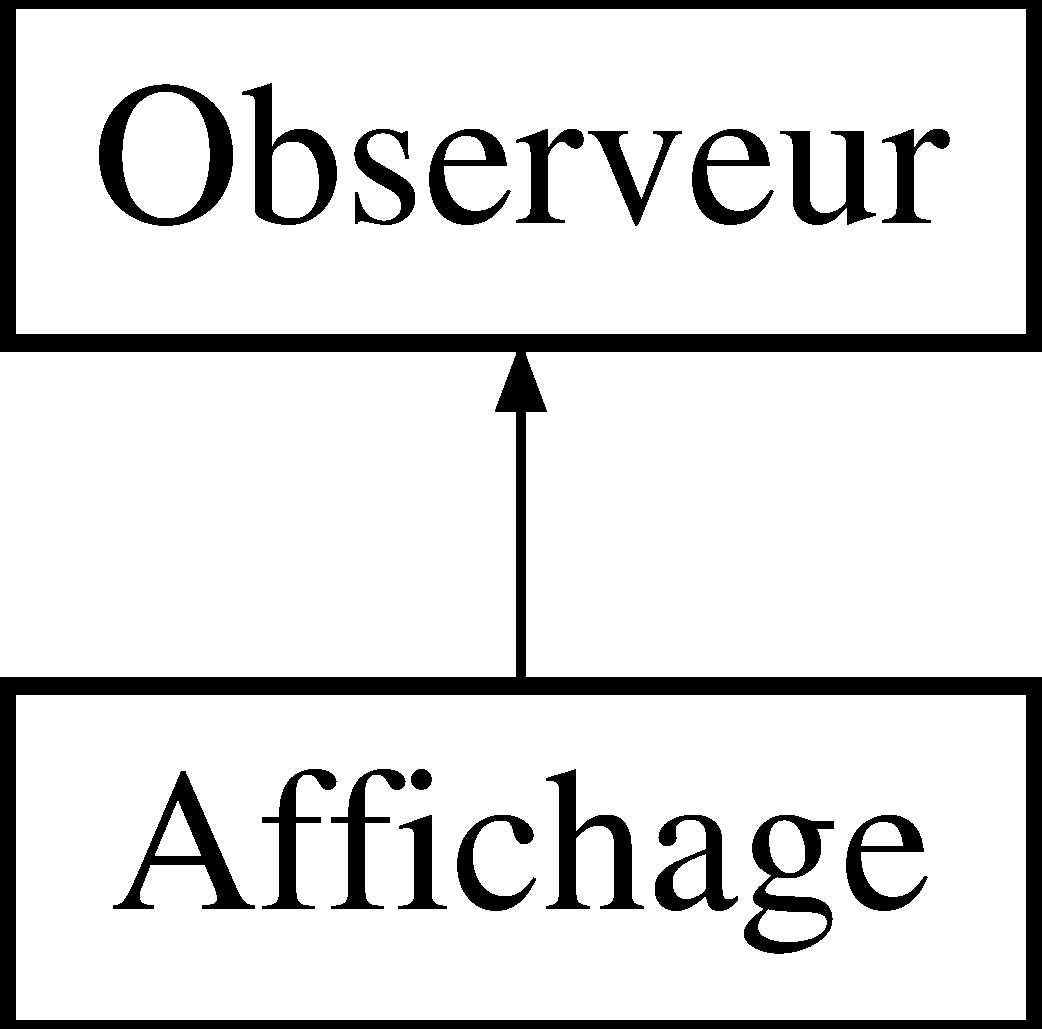
\includegraphics[height=2.000000cm]{class_observeur}
\end{center}
\end{figure}
\subsection*{Fonctions membres publiques}
\begin{DoxyCompactItemize}
\item 
virtual void \hyperlink{class_observeur_ad3f81ed71b0b056e7c20b731211c5958}{actualiser} ()=0
\begin{DoxyCompactList}\small\item\em Permet d'actualiser l'oserveur en fonction de son sujet. \end{DoxyCompactList}\end{DoxyCompactItemize}


\subsection{Description détaillée}
Classe \hyperlink{class_observeur}{Observeur} qui sert de base pour implementer des classes qui observent un sujet. 

\begin{DoxyDate}{Date}
15/11/2015 
\end{DoxyDate}
\begin{DoxyAuthor}{Auteur}
paul\-\_\-figiel 
\end{DoxyAuthor}


\subsection{Documentation des fonctions membres}
\hypertarget{class_observeur_ad3f81ed71b0b056e7c20b731211c5958}{\index{Observeur@{Observeur}!actualiser@{actualiser}}
\index{actualiser@{actualiser}!Observeur@{Observeur}}
\subsubsection[{actualiser}]{\setlength{\rightskip}{0pt plus 5cm}virtual void Observeur\-::actualiser (
\begin{DoxyParamCaption}
{}
\end{DoxyParamCaption}
)\hspace{0.3cm}{\ttfamily [pure virtual]}}}\label{class_observeur_ad3f81ed71b0b056e7c20b731211c5958}


Permet d'actualiser l'oserveur en fonction de son sujet. 



Implémenté dans \hyperlink{class_affichage_a76b52d63ae50d54a10bdc27370809a06}{Affichage}.



La documentation de cette classe a été générée à partir du fichier suivant \-:\begin{DoxyCompactItemize}
\item 
/home/figiel-\/paul/\-Bureau/\-Projet\-Poo/\-Projet\-P\-O\-O-\/\-A\-R\-A\-Y\-A-\/\-F\-I\-G\-I\-E\-L/include/\hyperlink{_observeur_8hpp}{Observeur.\-hpp}\end{DoxyCompactItemize}

\hypertarget{class_sujet}{\section{Référence de la classe Sujet}
\label{class_sujet}\index{Sujet@{Sujet}}
}


Classe \hyperlink{class_sujet}{Sujet} qui sert de base pour implementer des classes observées.  




{\ttfamily \#include $<$Sujet.\-hpp$>$}

Graphe d'héritage de Sujet\-:\begin{figure}[H]
\begin{center}
\leavevmode
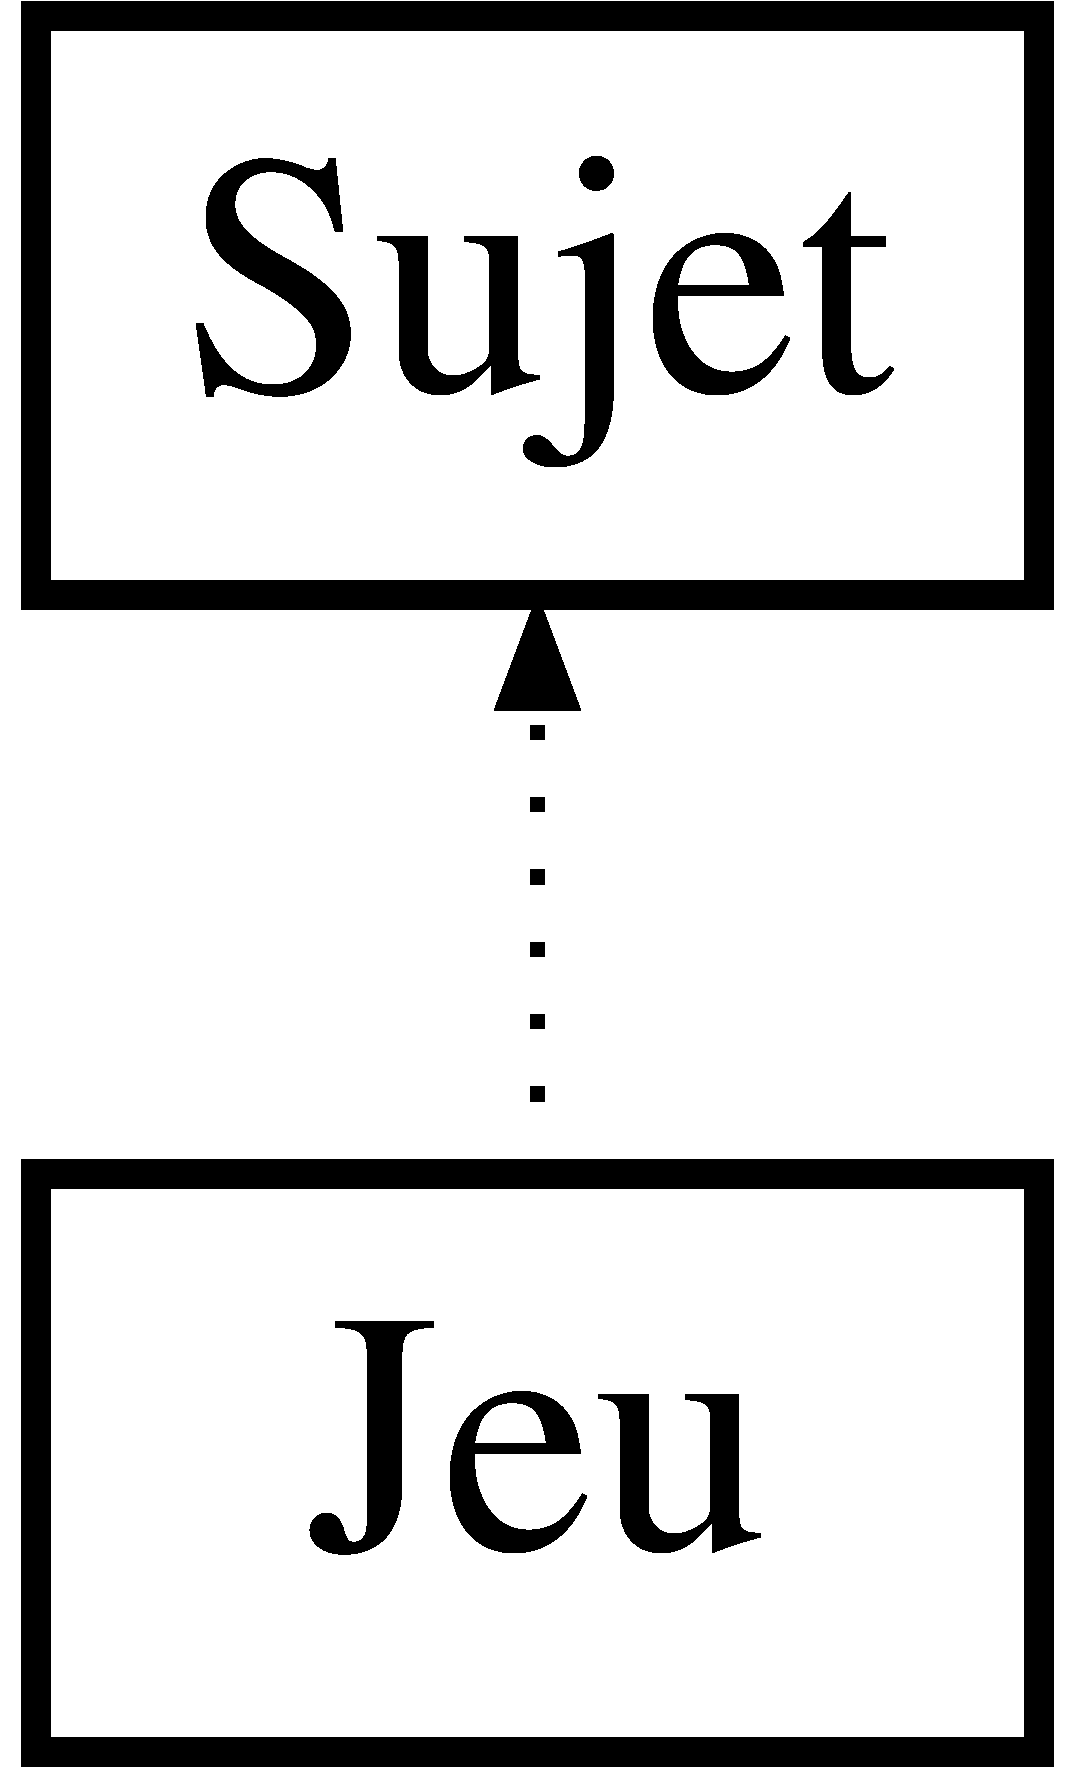
\includegraphics[height=2.000000cm]{class_sujet}
\end{center}
\end{figure}
\subsection*{Fonctions membres publiques}
\begin{DoxyCompactItemize}
\item 
virtual void \hyperlink{class_sujet_a77c41db2a06015ca931da1636e4dbc6d}{ajouter\-Obs} (\hyperlink{class_observeur}{Observeur} $\ast$o)=0
\begin{DoxyCompactList}\small\item\em Permet d'ajouter un observeur au sujet. \end{DoxyCompactList}\item 
virtual void \hyperlink{class_sujet_a84f5d1246b19042199924f90a69ec68b}{supprimer\-Obs} (int i)=0
\begin{DoxyCompactList}\small\item\em Permet de supprimer un observeur au sujet. \end{DoxyCompactList}\item 
virtual void \hyperlink{class_sujet_a28b5d0a1f6a476bfab9e12825a417179}{notifier\-Obs} ()=0
\begin{DoxyCompactList}\small\item\em Permet de notifier tous les observateurs du changement du sujet. \end{DoxyCompactList}\item 
virtual void \hyperlink{class_sujet_a895ceaa449463bd41526ee642569fbaa}{notifier\-Obs} (\hyperlink{class_observeur}{Observeur} $\ast$o)=0
\begin{DoxyCompactList}\small\item\em Permet de notifier un observeur. \end{DoxyCompactList}\end{DoxyCompactItemize}


\subsection{Description détaillée}
Classe \hyperlink{class_sujet}{Sujet} qui sert de base pour implementer des classes observées. 

\begin{DoxyDate}{Date}
15/11/2015 
\end{DoxyDate}
\begin{DoxyAuthor}{Auteur}
paul\-\_\-figiel 
\end{DoxyAuthor}


\subsection{Documentation des fonctions membres}
\hypertarget{class_sujet_a77c41db2a06015ca931da1636e4dbc6d}{\index{Sujet@{Sujet}!ajouter\-Obs@{ajouter\-Obs}}
\index{ajouter\-Obs@{ajouter\-Obs}!Sujet@{Sujet}}
\subsubsection[{ajouter\-Obs}]{\setlength{\rightskip}{0pt plus 5cm}virtual void Sujet\-::ajouter\-Obs (
\begin{DoxyParamCaption}
\item[{{\bf Observeur} $\ast$}]{o}
\end{DoxyParamCaption}
)\hspace{0.3cm}{\ttfamily [pure virtual]}}}\label{class_sujet_a77c41db2a06015ca931da1636e4dbc6d}


Permet d'ajouter un observeur au sujet. 


\begin{DoxyParams}{Paramètres}
{\em o} & \-: observeur à ajouter \\
\hline
\end{DoxyParams}


Implémenté dans \hyperlink{class_jeu_aee83ada0589e3352ec854b12e1c6e265}{Jeu}.

\hypertarget{class_sujet_a28b5d0a1f6a476bfab9e12825a417179}{\index{Sujet@{Sujet}!notifier\-Obs@{notifier\-Obs}}
\index{notifier\-Obs@{notifier\-Obs}!Sujet@{Sujet}}
\subsubsection[{notifier\-Obs}]{\setlength{\rightskip}{0pt plus 5cm}virtual void Sujet\-::notifier\-Obs (
\begin{DoxyParamCaption}
{}
\end{DoxyParamCaption}
)\hspace{0.3cm}{\ttfamily [pure virtual]}}}\label{class_sujet_a28b5d0a1f6a476bfab9e12825a417179}


Permet de notifier tous les observateurs du changement du sujet. 



Implémenté dans \hyperlink{class_jeu_ad955ffee4ed18add167fa957386a9821}{Jeu}.

\hypertarget{class_sujet_a895ceaa449463bd41526ee642569fbaa}{\index{Sujet@{Sujet}!notifier\-Obs@{notifier\-Obs}}
\index{notifier\-Obs@{notifier\-Obs}!Sujet@{Sujet}}
\subsubsection[{notifier\-Obs}]{\setlength{\rightskip}{0pt plus 5cm}virtual void Sujet\-::notifier\-Obs (
\begin{DoxyParamCaption}
\item[{{\bf Observeur} $\ast$}]{o}
\end{DoxyParamCaption}
)\hspace{0.3cm}{\ttfamily [pure virtual]}}}\label{class_sujet_a895ceaa449463bd41526ee642569fbaa}


Permet de notifier un observeur. 


\begin{DoxyParams}{Paramètres}
{\em o} & \-: observeur à notifier \\
\hline
\end{DoxyParams}


Implémenté dans \hyperlink{class_jeu_a56770ec2fa7af1cd5dfe1f06ee8d291a}{Jeu}.

\hypertarget{class_sujet_a84f5d1246b19042199924f90a69ec68b}{\index{Sujet@{Sujet}!supprimer\-Obs@{supprimer\-Obs}}
\index{supprimer\-Obs@{supprimer\-Obs}!Sujet@{Sujet}}
\subsubsection[{supprimer\-Obs}]{\setlength{\rightskip}{0pt plus 5cm}virtual void Sujet\-::supprimer\-Obs (
\begin{DoxyParamCaption}
\item[{int}]{i}
\end{DoxyParamCaption}
)\hspace{0.3cm}{\ttfamily [pure virtual]}}}\label{class_sujet_a84f5d1246b19042199924f90a69ec68b}


Permet de supprimer un observeur au sujet. 


\begin{DoxyParams}{Paramètres}
{\em o} & \-: indice de l'observateur à supprimer \\
\hline
\end{DoxyParams}


Implémenté dans \hyperlink{class_jeu_adbb1ba10c900ec336d744dbfd5de7f8e}{Jeu}.



La documentation de cette classe a été générée à partir du fichier suivant \-:\begin{DoxyCompactItemize}
\item 
/home/figiel-\/paul/\-Bureau/\-Projet\-Poo/\-Projet\-P\-O\-O-\/\-A\-R\-A\-Y\-A-\/\-F\-I\-G\-I\-E\-L/include/\hyperlink{_sujet_8hpp}{Sujet.\-hpp}\end{DoxyCompactItemize}

\chapter{Documentation des fichiers}
\hypertarget{_affichage_8hpp}{\section{Référence du fichier /home/figiel-\/paul/\-Bureau/\-Projet\-Poo/\-Projet\-P\-O\-O-\/\-A\-R\-A\-Y\-A-\/\-F\-I\-G\-I\-E\-L/include/\-Affichage.hpp}
\label{_affichage_8hpp}\index{/home/figiel-\/paul/\-Bureau/\-Projet\-Poo/\-Projet\-P\-O\-O-\/\-A\-R\-A\-Y\-A-\/\-F\-I\-G\-I\-E\-L/include/\-Affichage.\-hpp@{/home/figiel-\/paul/\-Bureau/\-Projet\-Poo/\-Projet\-P\-O\-O-\/\-A\-R\-A\-Y\-A-\/\-F\-I\-G\-I\-E\-L/include/\-Affichage.\-hpp}}
}


\hyperlink{class_affichage}{Affichage} graphique du jeu.  


{\ttfamily \#include $<$S\-F\-M\-L/\-Graphics.\-hpp$>$}\\*
{\ttfamily \#include $<$iostream$>$}\\*
{\ttfamily \#include \char`\"{}Observeur.\-hpp\char`\"{}}\\*
\subsection*{Classes}
\begin{DoxyCompactItemize}
\item 
class \hyperlink{class_affichage}{Affichage}
\begin{DoxyCompactList}\small\item\em Classe \hyperlink{class_affichage}{Affichage} qui sert à interpreter graphiquement l'état d'un objet \hyperlink{class_jeu}{Jeu}. \end{DoxyCompactList}\end{DoxyCompactItemize}
\subsection*{Macros}
\begin{DoxyCompactItemize}
\item 
\#define \hyperlink{_affichage_8hpp_a9b911fa287e90b56b503e284db0f390f}{A\-F\-F\-I\-C\-H\-A\-G\-E\-\_\-\-H\-P\-P}
\end{DoxyCompactItemize}
\subsection*{Variables}
\begin{DoxyCompactItemize}
\item 
int \hyperlink{_affichage_8hpp_a24c80669099d62cf0538af82c1cff466}{R\-E\-S\-X}
\item 
int \hyperlink{_affichage_8hpp_ac610e52e0fd370b03b49194aab3eae62}{R\-E\-S\-Y}
\item 
std\-::string \hyperlink{_affichage_8hpp_ac16a313eb3c00731761d1eb0854dca63}{N\-O\-M\-\_\-\-J\-E\-U}
\end{DoxyCompactItemize}


\subsection{Description détaillée}
\hyperlink{class_affichage}{Affichage} graphique du jeu. \begin{DoxyAuthor}{Auteur}
paul\-\_\-figiel 
\end{DoxyAuthor}
\begin{DoxyVersion}{Version}
1.\-0 
\end{DoxyVersion}


\subsection{Documentation des macros}
\hypertarget{_affichage_8hpp_a9b911fa287e90b56b503e284db0f390f}{\index{Affichage.\-hpp@{Affichage.\-hpp}!A\-F\-F\-I\-C\-H\-A\-G\-E\-\_\-\-H\-P\-P@{A\-F\-F\-I\-C\-H\-A\-G\-E\-\_\-\-H\-P\-P}}
\index{A\-F\-F\-I\-C\-H\-A\-G\-E\-\_\-\-H\-P\-P@{A\-F\-F\-I\-C\-H\-A\-G\-E\-\_\-\-H\-P\-P}!Affichage.hpp@{Affichage.\-hpp}}
\subsubsection[{A\-F\-F\-I\-C\-H\-A\-G\-E\-\_\-\-H\-P\-P}]{\setlength{\rightskip}{0pt plus 5cm}\#define A\-F\-F\-I\-C\-H\-A\-G\-E\-\_\-\-H\-P\-P}}\label{_affichage_8hpp_a9b911fa287e90b56b503e284db0f390f}


\subsection{Documentation des variables}
\hypertarget{_affichage_8hpp_ac16a313eb3c00731761d1eb0854dca63}{\index{Affichage.\-hpp@{Affichage.\-hpp}!N\-O\-M\-\_\-\-J\-E\-U@{N\-O\-M\-\_\-\-J\-E\-U}}
\index{N\-O\-M\-\_\-\-J\-E\-U@{N\-O\-M\-\_\-\-J\-E\-U}!Affichage.hpp@{Affichage.\-hpp}}
\subsubsection[{N\-O\-M\-\_\-\-J\-E\-U}]{\setlength{\rightskip}{0pt plus 5cm}std\-::string N\-O\-M\-\_\-\-J\-E\-U}}\label{_affichage_8hpp_ac16a313eb3c00731761d1eb0854dca63}
\hypertarget{_affichage_8hpp_a24c80669099d62cf0538af82c1cff466}{\index{Affichage.\-hpp@{Affichage.\-hpp}!R\-E\-S\-X@{R\-E\-S\-X}}
\index{R\-E\-S\-X@{R\-E\-S\-X}!Affichage.hpp@{Affichage.\-hpp}}
\subsubsection[{R\-E\-S\-X}]{\setlength{\rightskip}{0pt plus 5cm}int R\-E\-S\-X}}\label{_affichage_8hpp_a24c80669099d62cf0538af82c1cff466}
\hypertarget{_affichage_8hpp_ac610e52e0fd370b03b49194aab3eae62}{\index{Affichage.\-hpp@{Affichage.\-hpp}!R\-E\-S\-Y@{R\-E\-S\-Y}}
\index{R\-E\-S\-Y@{R\-E\-S\-Y}!Affichage.hpp@{Affichage.\-hpp}}
\subsubsection[{R\-E\-S\-Y}]{\setlength{\rightskip}{0pt plus 5cm}int R\-E\-S\-Y}}\label{_affichage_8hpp_ac610e52e0fd370b03b49194aab3eae62}

\hypertarget{_builder_deck_8hpp}{\section{Référence du fichier /home/figiel-\/paul/\-Bureau/\-Projet\-Poo/\-Projet\-P\-O\-O-\/\-A\-R\-A\-Y\-A-\/\-F\-I\-G\-I\-E\-L/include/\-Builder\-Deck.hpp}
\label{_builder_deck_8hpp}\index{/home/figiel-\/paul/\-Bureau/\-Projet\-Poo/\-Projet\-P\-O\-O-\/\-A\-R\-A\-Y\-A-\/\-F\-I\-G\-I\-E\-L/include/\-Builder\-Deck.\-hpp@{/home/figiel-\/paul/\-Bureau/\-Projet\-Poo/\-Projet\-P\-O\-O-\/\-A\-R\-A\-Y\-A-\/\-F\-I\-G\-I\-E\-L/include/\-Builder\-Deck.\-hpp}}
}


Implementation de la classe \hyperlink{class_builder_deck}{Builder\-Deck}.  


{\ttfamily \#include $<$iostream$>$}\\*
{\ttfamily \#include $<$fstream$>$}\\*
\subsection*{Classes}
\begin{DoxyCompactItemize}
\item 
class \hyperlink{class_builder_deck}{Builder\-Deck}
\begin{DoxyCompactList}\small\item\em Classe \hyperlink{class_builder_deck}{Builder\-Deck} qui permet de charger en memoire un deck composé de carte à partir de fichiers txt. \end{DoxyCompactList}\end{DoxyCompactItemize}


\subsection{Description détaillée}
Implementation de la classe \hyperlink{class_builder_deck}{Builder\-Deck}. \begin{DoxyAuthor}{Auteur}
paul\-\_\-figiel 
\end{DoxyAuthor}
\begin{DoxyVersion}{Version}
1.\-0 
\end{DoxyVersion}

\hypertarget{_builder_deck_txt_8hpp}{\section{Référence du fichier /home/figiel-\/paul/\-Bureau/\-Projet\-Poo/\-Projet\-P\-O\-O-\/\-A\-R\-A\-Y\-A-\/\-F\-I\-G\-I\-E\-L/include/\-Builder\-Deck\-Txt.hpp}
\label{_builder_deck_txt_8hpp}\index{/home/figiel-\/paul/\-Bureau/\-Projet\-Poo/\-Projet\-P\-O\-O-\/\-A\-R\-A\-Y\-A-\/\-F\-I\-G\-I\-E\-L/include/\-Builder\-Deck\-Txt.\-hpp@{/home/figiel-\/paul/\-Bureau/\-Projet\-Poo/\-Projet\-P\-O\-O-\/\-A\-R\-A\-Y\-A-\/\-F\-I\-G\-I\-E\-L/include/\-Builder\-Deck\-Txt.\-hpp}}
}


Implementation de la classe \hyperlink{class_builder_deck_txt}{Builder\-Deck\-Txt}.  


{\ttfamily \#include $<$iostream$>$}\\*
{\ttfamily \#include $<$fstream$>$}\\*
{\ttfamily \#include \char`\"{}Builder\-Deck.\-hpp\char`\"{}}\\*
\subsection*{Classes}
\begin{DoxyCompactItemize}
\item 
class \hyperlink{class_builder_deck_txt}{Builder\-Deck\-Txt}
\begin{DoxyCompactList}\small\item\em Classe \hyperlink{class_builder_deck_txt}{Builder\-Deck\-Txt} qui permet de charger en memoire un deck composé de carte à partir de fichiers txt. \end{DoxyCompactList}\end{DoxyCompactItemize}
\subsection*{Macros}
\begin{DoxyCompactItemize}
\item 
\#define \hyperlink{_builder_deck_txt_8hpp_a48927a2ec4e49e8a87a53bc006d2a3c2}{B\-U\-I\-L\-D\-E\-R\-D\-E\-C\-K\-T\-X\-T\-\_\-\-H\-P\-P}
\end{DoxyCompactItemize}


\subsection{Description détaillée}
Implementation de la classe \hyperlink{class_builder_deck_txt}{Builder\-Deck\-Txt}. \begin{DoxyAuthor}{Auteur}
paul\-\_\-figiel 
\end{DoxyAuthor}
\begin{DoxyVersion}{Version}
1.\-0 
\end{DoxyVersion}


\subsection{Documentation des macros}
\hypertarget{_builder_deck_txt_8hpp_a48927a2ec4e49e8a87a53bc006d2a3c2}{\index{Builder\-Deck\-Txt.\-hpp@{Builder\-Deck\-Txt.\-hpp}!B\-U\-I\-L\-D\-E\-R\-D\-E\-C\-K\-T\-X\-T\-\_\-\-H\-P\-P@{B\-U\-I\-L\-D\-E\-R\-D\-E\-C\-K\-T\-X\-T\-\_\-\-H\-P\-P}}
\index{B\-U\-I\-L\-D\-E\-R\-D\-E\-C\-K\-T\-X\-T\-\_\-\-H\-P\-P@{B\-U\-I\-L\-D\-E\-R\-D\-E\-C\-K\-T\-X\-T\-\_\-\-H\-P\-P}!BuilderDeckTxt.hpp@{Builder\-Deck\-Txt.\-hpp}}
\subsubsection[{B\-U\-I\-L\-D\-E\-R\-D\-E\-C\-K\-T\-X\-T\-\_\-\-H\-P\-P}]{\setlength{\rightskip}{0pt plus 5cm}\#define B\-U\-I\-L\-D\-E\-R\-D\-E\-C\-K\-T\-X\-T\-\_\-\-H\-P\-P}}\label{_builder_deck_txt_8hpp_a48927a2ec4e49e8a87a53bc006d2a3c2}

\hypertarget{_carte_8hpp}{\section{Référence du fichier /home/figiel-\/paul/\-Bureau/\-Projet\-Poo/\-Projet\-P\-O\-O-\/\-A\-R\-A\-Y\-A-\/\-F\-I\-G\-I\-E\-L/include/\-Carte.hpp}
\label{_carte_8hpp}\index{/home/figiel-\/paul/\-Bureau/\-Projet\-Poo/\-Projet\-P\-O\-O-\/\-A\-R\-A\-Y\-A-\/\-F\-I\-G\-I\-E\-L/include/\-Carte.\-hpp@{/home/figiel-\/paul/\-Bureau/\-Projet\-Poo/\-Projet\-P\-O\-O-\/\-A\-R\-A\-Y\-A-\/\-F\-I\-G\-I\-E\-L/include/\-Carte.\-hpp}}
}
{\ttfamily \#include $<$iostream$>$}\\*
{\ttfamily \#include $<$vector$>$}\\*
{\ttfamily \#include $<$Jeu.\-hpp$>$}\\*
\subsection*{Classes}
\begin{DoxyCompactItemize}
\item 
class \hyperlink{class_carte}{Carte}
\end{DoxyCompactItemize}

\hypertarget{_champion_8hpp}{\section{Référence du fichier /home/figiel-\/paul/\-Bureau/\-Projet\-Poo/\-Projet\-P\-O\-O-\/\-A\-R\-A\-Y\-A-\/\-F\-I\-G\-I\-E\-L/include/\-Champion.hpp}
\label{_champion_8hpp}\index{/home/figiel-\/paul/\-Bureau/\-Projet\-Poo/\-Projet\-P\-O\-O-\/\-A\-R\-A\-Y\-A-\/\-F\-I\-G\-I\-E\-L/include/\-Champion.\-hpp@{/home/figiel-\/paul/\-Bureau/\-Projet\-Poo/\-Projet\-P\-O\-O-\/\-A\-R\-A\-Y\-A-\/\-F\-I\-G\-I\-E\-L/include/\-Champion.\-hpp}}
}
{\ttfamily \#include $<$iostream$>$}\\*
{\ttfamily \#include $<$math.\-h$>$}\\*
\subsection*{Classes}
\begin{DoxyCompactItemize}
\item 
class \hyperlink{class_champion}{Champion}
\end{DoxyCompactItemize}

\hypertarget{_deck_8hpp}{\section{Référence du fichier /home/figiel-\/paul/\-Bureau/\-Projet\-Poo/\-Projet\-P\-O\-O-\/\-A\-R\-A\-Y\-A-\/\-F\-I\-G\-I\-E\-L/include/\-Deck.hpp}
\label{_deck_8hpp}\index{/home/figiel-\/paul/\-Bureau/\-Projet\-Poo/\-Projet\-P\-O\-O-\/\-A\-R\-A\-Y\-A-\/\-F\-I\-G\-I\-E\-L/include/\-Deck.\-hpp@{/home/figiel-\/paul/\-Bureau/\-Projet\-Poo/\-Projet\-P\-O\-O-\/\-A\-R\-A\-Y\-A-\/\-F\-I\-G\-I\-E\-L/include/\-Deck.\-hpp}}
}
{\ttfamily \#include $<$vector$>$}\\*
\subsection*{Classes}
\begin{DoxyCompactItemize}
\item 
class \hyperlink{class_deck}{Deck}
\end{DoxyCompactItemize}

\hypertarget{_director_8hpp}{\section{Référence du fichier /home/figiel-\/paul/\-Bureau/\-Projet\-Poo/\-Projet\-P\-O\-O-\/\-A\-R\-A\-Y\-A-\/\-F\-I\-G\-I\-E\-L/include/\-Director.hpp}
\label{_director_8hpp}\index{/home/figiel-\/paul/\-Bureau/\-Projet\-Poo/\-Projet\-P\-O\-O-\/\-A\-R\-A\-Y\-A-\/\-F\-I\-G\-I\-E\-L/include/\-Director.\-hpp@{/home/figiel-\/paul/\-Bureau/\-Projet\-Poo/\-Projet\-P\-O\-O-\/\-A\-R\-A\-Y\-A-\/\-F\-I\-G\-I\-E\-L/include/\-Director.\-hpp}}
}


Gere les builder de carte.  


\subsection*{Classes}
\begin{DoxyCompactItemize}
\item 
class \hyperlink{class_director}{Director}
\begin{DoxyCompactList}\small\item\em Classe \hyperlink{class_director}{Director} qui sert à gerer les builder de carte. \end{DoxyCompactList}\end{DoxyCompactItemize}


\subsection{Description détaillée}
Gere les builder de carte. \begin{DoxyAuthor}{Auteur}
paul\-\_\-figiel 
\end{DoxyAuthor}
\begin{DoxyVersion}{Version}
1.\-0 
\end{DoxyVersion}

\hypertarget{_director_concret_8hpp}{\section{Référence du fichier /home/figiel-\/paul/\-Bureau/\-Projet\-Poo/\-Projet\-P\-O\-O-\/\-A\-R\-A\-Y\-A-\/\-F\-I\-G\-I\-E\-L/include/\-Director\-Concret.hpp}
\label{_director_concret_8hpp}\index{/home/figiel-\/paul/\-Bureau/\-Projet\-Poo/\-Projet\-P\-O\-O-\/\-A\-R\-A\-Y\-A-\/\-F\-I\-G\-I\-E\-L/include/\-Director\-Concret.\-hpp@{/home/figiel-\/paul/\-Bureau/\-Projet\-Poo/\-Projet\-P\-O\-O-\/\-A\-R\-A\-Y\-A-\/\-F\-I\-G\-I\-E\-L/include/\-Director\-Concret.\-hpp}}
}


Gere les builder de carte.  


{\ttfamily \#include \char`\"{}Director.\-hpp\char`\"{}}\\*
\subsection*{Classes}
\begin{DoxyCompactItemize}
\item 
class \hyperlink{class_director_concret}{Director\-Concret}
\begin{DoxyCompactList}\small\item\em Classe \hyperlink{class_director_concret}{Director\-Concret} qui sert à gerer les builder de carte, implemente \hyperlink{class_director}{Director}. \end{DoxyCompactList}\end{DoxyCompactItemize}
\subsection*{Macros}
\begin{DoxyCompactItemize}
\item 
\#define \hyperlink{_director_concret_8hpp_ac03667b6a296c9f33f4f3e7a97ea5061}{D\-I\-R\-E\-C\-T\-O\-R\-C\-O\-N\-C\-R\-E\-T\-\_\-\-H\-P\-P}
\end{DoxyCompactItemize}


\subsection{Description détaillée}
Gere les builder de carte. \begin{DoxyAuthor}{Auteur}
paul\-\_\-figiel 
\end{DoxyAuthor}
\begin{DoxyVersion}{Version}
1.\-0 
\end{DoxyVersion}


\subsection{Documentation des macros}
\hypertarget{_director_concret_8hpp_ac03667b6a296c9f33f4f3e7a97ea5061}{\index{Director\-Concret.\-hpp@{Director\-Concret.\-hpp}!D\-I\-R\-E\-C\-T\-O\-R\-C\-O\-N\-C\-R\-E\-T\-\_\-\-H\-P\-P@{D\-I\-R\-E\-C\-T\-O\-R\-C\-O\-N\-C\-R\-E\-T\-\_\-\-H\-P\-P}}
\index{D\-I\-R\-E\-C\-T\-O\-R\-C\-O\-N\-C\-R\-E\-T\-\_\-\-H\-P\-P@{D\-I\-R\-E\-C\-T\-O\-R\-C\-O\-N\-C\-R\-E\-T\-\_\-\-H\-P\-P}!DirectorConcret.hpp@{Director\-Concret.\-hpp}}
\subsubsection[{D\-I\-R\-E\-C\-T\-O\-R\-C\-O\-N\-C\-R\-E\-T\-\_\-\-H\-P\-P}]{\setlength{\rightskip}{0pt plus 5cm}\#define D\-I\-R\-E\-C\-T\-O\-R\-C\-O\-N\-C\-R\-E\-T\-\_\-\-H\-P\-P}}\label{_director_concret_8hpp_ac03667b6a296c9f33f4f3e7a97ea5061}

\hypertarget{_effet_8hpp}{\section{Référence du fichier /home/figiel-\/paul/\-Bureau/\-Projet\-Poo/\-Projet\-P\-O\-O-\/\-A\-R\-A\-Y\-A-\/\-F\-I\-G\-I\-E\-L/include/\-Effet.hpp}
\label{_effet_8hpp}\index{/home/figiel-\/paul/\-Bureau/\-Projet\-Poo/\-Projet\-P\-O\-O-\/\-A\-R\-A\-Y\-A-\/\-F\-I\-G\-I\-E\-L/include/\-Effet.\-hpp@{/home/figiel-\/paul/\-Bureau/\-Projet\-Poo/\-Projet\-P\-O\-O-\/\-A\-R\-A\-Y\-A-\/\-F\-I\-G\-I\-E\-L/include/\-Effet.\-hpp}}
}
{\ttfamily \#include $<$iostream$>$}\\*
{\ttfamily \#include $<$cstdlib$>$}\\*
{\ttfamily \#include $<$ctime$>$}\\*
\subsection*{Classes}
\begin{DoxyCompactItemize}
\item 
class \hyperlink{class_effet}{Effet}
\end{DoxyCompactItemize}

\hypertarget{_effet_boost_8hpp}{\section{Référence du fichier /home/figiel-\/paul/\-Bureau/\-Projet\-Poo/\-Projet\-P\-O\-O-\/\-A\-R\-A\-Y\-A-\/\-F\-I\-G\-I\-E\-L/include/\-Effet\-Boost.hpp}
\label{_effet_boost_8hpp}\index{/home/figiel-\/paul/\-Bureau/\-Projet\-Poo/\-Projet\-P\-O\-O-\/\-A\-R\-A\-Y\-A-\/\-F\-I\-G\-I\-E\-L/include/\-Effet\-Boost.\-hpp@{/home/figiel-\/paul/\-Bureau/\-Projet\-Poo/\-Projet\-P\-O\-O-\/\-A\-R\-A\-Y\-A-\/\-F\-I\-G\-I\-E\-L/include/\-Effet\-Boost.\-hpp}}
}
{\ttfamily \#include $<$iostream$>$}\\*
{\ttfamily \#include \char`\"{}Effet.\-hpp\char`\"{}}\\*
\subsection*{Classes}
\begin{DoxyCompactItemize}
\item 
class \hyperlink{class_effet_boost}{Effet\-Boost}
\end{DoxyCompactItemize}
\subsection*{Macros}
\begin{DoxyCompactItemize}
\item 
\#define \hyperlink{_effet_boost_8hpp_a0ea64f4c9da5e50126829699566e6f27}{E\-F\-F\-E\-T\-B\-O\-O\-S\-T\-\_\-\-H\-P\-P}
\end{DoxyCompactItemize}


\subsection{Documentation des macros}
\hypertarget{_effet_boost_8hpp_a0ea64f4c9da5e50126829699566e6f27}{\index{Effet\-Boost.\-hpp@{Effet\-Boost.\-hpp}!E\-F\-F\-E\-T\-B\-O\-O\-S\-T\-\_\-\-H\-P\-P@{E\-F\-F\-E\-T\-B\-O\-O\-S\-T\-\_\-\-H\-P\-P}}
\index{E\-F\-F\-E\-T\-B\-O\-O\-S\-T\-\_\-\-H\-P\-P@{E\-F\-F\-E\-T\-B\-O\-O\-S\-T\-\_\-\-H\-P\-P}!EffetBoost.hpp@{Effet\-Boost.\-hpp}}
\subsubsection[{E\-F\-F\-E\-T\-B\-O\-O\-S\-T\-\_\-\-H\-P\-P}]{\setlength{\rightskip}{0pt plus 5cm}\#define E\-F\-F\-E\-T\-B\-O\-O\-S\-T\-\_\-\-H\-P\-P}}\label{_effet_boost_8hpp_a0ea64f4c9da5e50126829699566e6f27}

\hypertarget{_effet_endurant_8hpp}{\section{Référence du fichier /home/figiel-\/paul/\-Bureau/\-Projet\-Poo/\-Projet\-P\-O\-O-\/\-A\-R\-A\-Y\-A-\/\-F\-I\-G\-I\-E\-L/include/\-Effet\-Endurant.hpp}
\label{_effet_endurant_8hpp}\index{/home/figiel-\/paul/\-Bureau/\-Projet\-Poo/\-Projet\-P\-O\-O-\/\-A\-R\-A\-Y\-A-\/\-F\-I\-G\-I\-E\-L/include/\-Effet\-Endurant.\-hpp@{/home/figiel-\/paul/\-Bureau/\-Projet\-Poo/\-Projet\-P\-O\-O-\/\-A\-R\-A\-Y\-A-\/\-F\-I\-G\-I\-E\-L/include/\-Effet\-Endurant.\-hpp}}
}
{\ttfamily \#include $<$iostream$>$}\\*
{\ttfamily \#include \char`\"{}Effet.\-hpp\char`\"{}}\\*
\subsection*{Classes}
\begin{DoxyCompactItemize}
\item 
class \hyperlink{class_effet_endurant}{Effet\-Endurant}
\end{DoxyCompactItemize}

\hypertarget{_effet_finisher_8hpp}{\section{Référence du fichier /home/figiel-\/paul/\-Bureau/\-Projet\-Poo/\-Projet\-P\-O\-O-\/\-A\-R\-A\-Y\-A-\/\-F\-I\-G\-I\-E\-L/include/\-Effet\-Finisher.hpp}
\label{_effet_finisher_8hpp}\index{/home/figiel-\/paul/\-Bureau/\-Projet\-Poo/\-Projet\-P\-O\-O-\/\-A\-R\-A\-Y\-A-\/\-F\-I\-G\-I\-E\-L/include/\-Effet\-Finisher.\-hpp@{/home/figiel-\/paul/\-Bureau/\-Projet\-Poo/\-Projet\-P\-O\-O-\/\-A\-R\-A\-Y\-A-\/\-F\-I\-G\-I\-E\-L/include/\-Effet\-Finisher.\-hpp}}
}
{\ttfamily \#include $<$iostream$>$}\\*
{\ttfamily \#include \char`\"{}Effet.\-hpp\char`\"{}}\\*
\subsection*{Classes}
\begin{DoxyCompactItemize}
\item 
class \hyperlink{class_effet_finisher}{Effet\-Finisher}
\end{DoxyCompactItemize}

\hypertarget{_effet_link_8hpp}{\section{Référence du fichier /home/figiel-\/paul/\-Bureau/\-Projet\-Poo/\-Projet\-P\-O\-O-\/\-A\-R\-A\-Y\-A-\/\-F\-I\-G\-I\-E\-L/include/\-Effet\-Link.hpp}
\label{_effet_link_8hpp}\index{/home/figiel-\/paul/\-Bureau/\-Projet\-Poo/\-Projet\-P\-O\-O-\/\-A\-R\-A\-Y\-A-\/\-F\-I\-G\-I\-E\-L/include/\-Effet\-Link.\-hpp@{/home/figiel-\/paul/\-Bureau/\-Projet\-Poo/\-Projet\-P\-O\-O-\/\-A\-R\-A\-Y\-A-\/\-F\-I\-G\-I\-E\-L/include/\-Effet\-Link.\-hpp}}
}
{\ttfamily \#include $<$iostream$>$}\\*
{\ttfamily \#include \char`\"{}Effet.\-hpp\char`\"{}}\\*
\subsection*{Classes}
\begin{DoxyCompactItemize}
\item 
class \hyperlink{class_effet_link}{Effet\-Link}
\end{DoxyCompactItemize}

\hypertarget{_effet_return_8hpp}{\section{Référence du fichier /home/figiel-\/paul/\-Bureau/\-Projet\-Poo/\-Projet\-P\-O\-O-\/\-A\-R\-A\-Y\-A-\/\-F\-I\-G\-I\-E\-L/include/\-Effet\-Return.hpp}
\label{_effet_return_8hpp}\index{/home/figiel-\/paul/\-Bureau/\-Projet\-Poo/\-Projet\-P\-O\-O-\/\-A\-R\-A\-Y\-A-\/\-F\-I\-G\-I\-E\-L/include/\-Effet\-Return.\-hpp@{/home/figiel-\/paul/\-Bureau/\-Projet\-Poo/\-Projet\-P\-O\-O-\/\-A\-R\-A\-Y\-A-\/\-F\-I\-G\-I\-E\-L/include/\-Effet\-Return.\-hpp}}
}
{\ttfamily \#include $<$iostream$>$}\\*
{\ttfamily \#include \char`\"{}Effet.\-hpp\char`\"{}}\\*
\subsection*{Classes}
\begin{DoxyCompactItemize}
\item 
class \hyperlink{class_effet_return}{Effet\-Return}
\end{DoxyCompactItemize}

\hypertarget{_effet_the_answer_8hpp}{\section{Référence du fichier /home/figiel-\/paul/\-Bureau/\-Projet\-Poo/\-Projet\-P\-O\-O-\/\-A\-R\-A\-Y\-A-\/\-F\-I\-G\-I\-E\-L/include/\-Effet\-The\-Answer.hpp}
\label{_effet_the_answer_8hpp}\index{/home/figiel-\/paul/\-Bureau/\-Projet\-Poo/\-Projet\-P\-O\-O-\/\-A\-R\-A\-Y\-A-\/\-F\-I\-G\-I\-E\-L/include/\-Effet\-The\-Answer.\-hpp@{/home/figiel-\/paul/\-Bureau/\-Projet\-Poo/\-Projet\-P\-O\-O-\/\-A\-R\-A\-Y\-A-\/\-F\-I\-G\-I\-E\-L/include/\-Effet\-The\-Answer.\-hpp}}
}
{\ttfamily \#include $<$iostream$>$}\\*
{\ttfamily \#include \char`\"{}Effet.\-hpp\char`\"{}}\\*
\subsection*{Classes}
\begin{DoxyCompactItemize}
\item 
class \hyperlink{class_effet_the_answer}{Effet\-The\-Answer}
\end{DoxyCompactItemize}

\hypertarget{_effet_yolo_8hpp}{\section{Référence du fichier /home/figiel-\/paul/\-Bureau/\-Projet\-Poo/\-Projet\-P\-O\-O-\/\-A\-R\-A\-Y\-A-\/\-F\-I\-G\-I\-E\-L/include/\-Effet\-Yolo.hpp}
\label{_effet_yolo_8hpp}\index{/home/figiel-\/paul/\-Bureau/\-Projet\-Poo/\-Projet\-P\-O\-O-\/\-A\-R\-A\-Y\-A-\/\-F\-I\-G\-I\-E\-L/include/\-Effet\-Yolo.\-hpp@{/home/figiel-\/paul/\-Bureau/\-Projet\-Poo/\-Projet\-P\-O\-O-\/\-A\-R\-A\-Y\-A-\/\-F\-I\-G\-I\-E\-L/include/\-Effet\-Yolo.\-hpp}}
}
{\ttfamily \#include $<$iostream$>$}\\*
{\ttfamily \#include \char`\"{}Effet.\-hpp\char`\"{}}\\*
\subsection*{Classes}
\begin{DoxyCompactItemize}
\item 
class \hyperlink{class_effet_yolo}{Effet\-Yolo}
\end{DoxyCompactItemize}

\hypertarget{_etat_8hpp}{\section{Référence du fichier /home/figiel-\/paul/\-Bureau/\-Projet\-Poo/\-Projet\-P\-O\-O-\/\-A\-R\-A\-Y\-A-\/\-F\-I\-G\-I\-E\-L/include/\-Etat.hpp}
\label{_etat_8hpp}\index{/home/figiel-\/paul/\-Bureau/\-Projet\-Poo/\-Projet\-P\-O\-O-\/\-A\-R\-A\-Y\-A-\/\-F\-I\-G\-I\-E\-L/include/\-Etat.\-hpp@{/home/figiel-\/paul/\-Bureau/\-Projet\-Poo/\-Projet\-P\-O\-O-\/\-A\-R\-A\-Y\-A-\/\-F\-I\-G\-I\-E\-L/include/\-Etat.\-hpp}}
}
{\ttfamily \#include $<$iostream$>$}\\*
{\ttfamily \#include $<$vector$>$}\\*
\subsection*{Classes}
\begin{DoxyCompactItemize}
\item 
class \hyperlink{class_etat}{Etat}
\end{DoxyCompactItemize}

\hypertarget{_etat_bluff_8hpp}{\section{Référence du fichier /home/figiel-\/paul/\-Bureau/\-Projet\-Poo/\-Projet\-P\-O\-O-\/\-A\-R\-A\-Y\-A-\/\-F\-I\-G\-I\-E\-L/include/\-Etat\-Bluff.hpp}
\label{_etat_bluff_8hpp}\index{/home/figiel-\/paul/\-Bureau/\-Projet\-Poo/\-Projet\-P\-O\-O-\/\-A\-R\-A\-Y\-A-\/\-F\-I\-G\-I\-E\-L/include/\-Etat\-Bluff.\-hpp@{/home/figiel-\/paul/\-Bureau/\-Projet\-Poo/\-Projet\-P\-O\-O-\/\-A\-R\-A\-Y\-A-\/\-F\-I\-G\-I\-E\-L/include/\-Etat\-Bluff.\-hpp}}
}
{\ttfamily \#include $<$iostream$>$}\\*
{\ttfamily \#include \char`\"{}Etat.\-hpp\char`\"{}}\\*
\subsection*{Classes}
\begin{DoxyCompactItemize}
\item 
class \hyperlink{class_etat_bluff}{Etat\-Bluff}
\end{DoxyCompactItemize}
\subsection*{Macros}
\begin{DoxyCompactItemize}
\item 
\#define \hyperlink{_etat_bluff_8hpp_ae92ac26d9240f7dfb651f513badf1797}{E\-T\-A\-T\-B\-L\-U\-F\-F\-\_\-\-H\-P\-P}
\end{DoxyCompactItemize}


\subsection{Documentation des macros}
\hypertarget{_etat_bluff_8hpp_ae92ac26d9240f7dfb651f513badf1797}{\index{Etat\-Bluff.\-hpp@{Etat\-Bluff.\-hpp}!E\-T\-A\-T\-B\-L\-U\-F\-F\-\_\-\-H\-P\-P@{E\-T\-A\-T\-B\-L\-U\-F\-F\-\_\-\-H\-P\-P}}
\index{E\-T\-A\-T\-B\-L\-U\-F\-F\-\_\-\-H\-P\-P@{E\-T\-A\-T\-B\-L\-U\-F\-F\-\_\-\-H\-P\-P}!EtatBluff.hpp@{Etat\-Bluff.\-hpp}}
\subsubsection[{E\-T\-A\-T\-B\-L\-U\-F\-F\-\_\-\-H\-P\-P}]{\setlength{\rightskip}{0pt plus 5cm}\#define E\-T\-A\-T\-B\-L\-U\-F\-F\-\_\-\-H\-P\-P}}\label{_etat_bluff_8hpp_ae92ac26d9240f7dfb651f513badf1797}

\hypertarget{_etat_calc_dmg_8hpp}{\section{Référence du fichier /home/figiel-\/paul/\-Bureau/\-Projet\-Poo/\-Projet\-P\-O\-O-\/\-A\-R\-A\-Y\-A-\/\-F\-I\-G\-I\-E\-L/include/\-Etat\-Calc\-Dmg.hpp}
\label{_etat_calc_dmg_8hpp}\index{/home/figiel-\/paul/\-Bureau/\-Projet\-Poo/\-Projet\-P\-O\-O-\/\-A\-R\-A\-Y\-A-\/\-F\-I\-G\-I\-E\-L/include/\-Etat\-Calc\-Dmg.\-hpp@{/home/figiel-\/paul/\-Bureau/\-Projet\-Poo/\-Projet\-P\-O\-O-\/\-A\-R\-A\-Y\-A-\/\-F\-I\-G\-I\-E\-L/include/\-Etat\-Calc\-Dmg.\-hpp}}
}
{\ttfamily \#include $<$iostream$>$}\\*
{\ttfamily \#include \char`\"{}Etat.\-hpp\char`\"{}}\\*
\subsection*{Classes}
\begin{DoxyCompactItemize}
\item 
class \hyperlink{class_etat_calc_dmg}{Etat\-Calc\-Dmg}
\end{DoxyCompactItemize}

\hypertarget{_etat_choix_j1_8hpp}{\section{Référence du fichier /home/figiel-\/paul/\-Bureau/\-Projet\-Poo/\-Projet\-P\-O\-O-\/\-A\-R\-A\-Y\-A-\/\-F\-I\-G\-I\-E\-L/include/\-Etat\-Choix\-J1.hpp}
\label{_etat_choix_j1_8hpp}\index{/home/figiel-\/paul/\-Bureau/\-Projet\-Poo/\-Projet\-P\-O\-O-\/\-A\-R\-A\-Y\-A-\/\-F\-I\-G\-I\-E\-L/include/\-Etat\-Choix\-J1.\-hpp@{/home/figiel-\/paul/\-Bureau/\-Projet\-Poo/\-Projet\-P\-O\-O-\/\-A\-R\-A\-Y\-A-\/\-F\-I\-G\-I\-E\-L/include/\-Etat\-Choix\-J1.\-hpp}}
}
{\ttfamily \#include $<$iostream$>$}\\*
{\ttfamily \#include \char`\"{}Etat.\-hpp\char`\"{}}\\*
\subsection*{Classes}
\begin{DoxyCompactItemize}
\item 
class \hyperlink{class_etat_choix_j1}{Etat\-Choix\-J1}
\end{DoxyCompactItemize}

\hypertarget{_etat_choix_j2_8hpp}{\section{Référence du fichier /home/figiel-\/paul/\-Bureau/\-Projet\-Poo/\-Projet\-P\-O\-O-\/\-A\-R\-A\-Y\-A-\/\-F\-I\-G\-I\-E\-L/include/\-Etat\-Choix\-J2.hpp}
\label{_etat_choix_j2_8hpp}\index{/home/figiel-\/paul/\-Bureau/\-Projet\-Poo/\-Projet\-P\-O\-O-\/\-A\-R\-A\-Y\-A-\/\-F\-I\-G\-I\-E\-L/include/\-Etat\-Choix\-J2.\-hpp@{/home/figiel-\/paul/\-Bureau/\-Projet\-Poo/\-Projet\-P\-O\-O-\/\-A\-R\-A\-Y\-A-\/\-F\-I\-G\-I\-E\-L/include/\-Etat\-Choix\-J2.\-hpp}}
}
{\ttfamily \#include $<$iostream$>$}\\*
{\ttfamily \#include \char`\"{}Etat.\-hpp\char`\"{}}\\*
\subsection*{Classes}
\begin{DoxyCompactItemize}
\item 
class \hyperlink{class_etat_choix_j2}{Etat\-Choix\-J2}
\end{DoxyCompactItemize}

\hypertarget{_etat_choix_perso_8hpp}{\section{Référence du fichier /home/figiel-\/paul/\-Bureau/\-Projet\-Poo/\-Projet\-P\-O\-O-\/\-A\-R\-A\-Y\-A-\/\-F\-I\-G\-I\-E\-L/include/\-Etat\-Choix\-Perso.hpp}
\label{_etat_choix_perso_8hpp}\index{/home/figiel-\/paul/\-Bureau/\-Projet\-Poo/\-Projet\-P\-O\-O-\/\-A\-R\-A\-Y\-A-\/\-F\-I\-G\-I\-E\-L/include/\-Etat\-Choix\-Perso.\-hpp@{/home/figiel-\/paul/\-Bureau/\-Projet\-Poo/\-Projet\-P\-O\-O-\/\-A\-R\-A\-Y\-A-\/\-F\-I\-G\-I\-E\-L/include/\-Etat\-Choix\-Perso.\-hpp}}
}
{\ttfamily \#include $<$iostream$>$}\\*
{\ttfamily \#include \char`\"{}Etat.\-hpp\char`\"{}}\\*
\subsection*{Classes}
\begin{DoxyCompactItemize}
\item 
class \hyperlink{class_etat_choix_perso}{Etat\-Choix\-Perso}
\end{DoxyCompactItemize}

\hypertarget{_etat_choix_win_8hpp}{\section{Référence du fichier /home/figiel-\/paul/\-Bureau/\-Projet\-Poo/\-Projet\-P\-O\-O-\/\-A\-R\-A\-Y\-A-\/\-F\-I\-G\-I\-E\-L/include/\-Etat\-Choix\-Win.hpp}
\label{_etat_choix_win_8hpp}\index{/home/figiel-\/paul/\-Bureau/\-Projet\-Poo/\-Projet\-P\-O\-O-\/\-A\-R\-A\-Y\-A-\/\-F\-I\-G\-I\-E\-L/include/\-Etat\-Choix\-Win.\-hpp@{/home/figiel-\/paul/\-Bureau/\-Projet\-Poo/\-Projet\-P\-O\-O-\/\-A\-R\-A\-Y\-A-\/\-F\-I\-G\-I\-E\-L/include/\-Etat\-Choix\-Win.\-hpp}}
}
{\ttfamily \#include $<$iostream$>$}\\*
{\ttfamily \#include \char`\"{}Etat.\-hpp\char`\"{}}\\*
\subsection*{Classes}
\begin{DoxyCompactItemize}
\item 
class \hyperlink{class_etat_choix_win}{Etat\-Choix\-Win}
\end{DoxyCompactItemize}

\hypertarget{_etat_clean_up_8hpp}{\section{Référence du fichier /home/figiel-\/paul/\-Bureau/\-Projet\-Poo/\-Projet\-P\-O\-O-\/\-A\-R\-A\-Y\-A-\/\-F\-I\-G\-I\-E\-L/include/\-Etat\-Clean\-Up.hpp}
\label{_etat_clean_up_8hpp}\index{/home/figiel-\/paul/\-Bureau/\-Projet\-Poo/\-Projet\-P\-O\-O-\/\-A\-R\-A\-Y\-A-\/\-F\-I\-G\-I\-E\-L/include/\-Etat\-Clean\-Up.\-hpp@{/home/figiel-\/paul/\-Bureau/\-Projet\-Poo/\-Projet\-P\-O\-O-\/\-A\-R\-A\-Y\-A-\/\-F\-I\-G\-I\-E\-L/include/\-Etat\-Clean\-Up.\-hpp}}
}
{\ttfamily \#include $<$iostream$>$}\\*
{\ttfamily \#include \char`\"{}Etat.\-hpp\char`\"{}}\\*
\subsection*{Classes}
\begin{DoxyCompactItemize}
\item 
class \hyperlink{class_etat_clean_up}{Etat\-Clean\-Up}
\end{DoxyCompactItemize}

\hypertarget{_etat_combo_8hpp}{\section{Référence du fichier /home/figiel-\/paul/\-Bureau/\-Projet\-Poo/\-Projet\-P\-O\-O-\/\-A\-R\-A\-Y\-A-\/\-F\-I\-G\-I\-E\-L/include/\-Etat\-Combo.hpp}
\label{_etat_combo_8hpp}\index{/home/figiel-\/paul/\-Bureau/\-Projet\-Poo/\-Projet\-P\-O\-O-\/\-A\-R\-A\-Y\-A-\/\-F\-I\-G\-I\-E\-L/include/\-Etat\-Combo.\-hpp@{/home/figiel-\/paul/\-Bureau/\-Projet\-Poo/\-Projet\-P\-O\-O-\/\-A\-R\-A\-Y\-A-\/\-F\-I\-G\-I\-E\-L/include/\-Etat\-Combo.\-hpp}}
}
{\ttfamily \#include $<$iostream$>$}\\*
{\ttfamily \#include \char`\"{}Etat.\-hpp\char`\"{}}\\*
\subsection*{Classes}
\begin{DoxyCompactItemize}
\item 
class \hyperlink{class_etat_combo}{Etat\-Combo}
\end{DoxyCompactItemize}

\hypertarget{_etat_fin_8hpp}{\section{Référence du fichier /home/figiel-\/paul/\-Bureau/\-Projet\-Poo/\-Projet\-P\-O\-O-\/\-A\-R\-A\-Y\-A-\/\-F\-I\-G\-I\-E\-L/include/\-Etat\-Fin.hpp}
\label{_etat_fin_8hpp}\index{/home/figiel-\/paul/\-Bureau/\-Projet\-Poo/\-Projet\-P\-O\-O-\/\-A\-R\-A\-Y\-A-\/\-F\-I\-G\-I\-E\-L/include/\-Etat\-Fin.\-hpp@{/home/figiel-\/paul/\-Bureau/\-Projet\-Poo/\-Projet\-P\-O\-O-\/\-A\-R\-A\-Y\-A-\/\-F\-I\-G\-I\-E\-L/include/\-Etat\-Fin.\-hpp}}
}
{\ttfamily \#include $<$iostream$>$}\\*
{\ttfamily \#include \char`\"{}Etat.\-hpp\char`\"{}}\\*
\subsection*{Classes}
\begin{DoxyCompactItemize}
\item 
class \hyperlink{class_etat_fin}{Etat\-Fin}
\end{DoxyCompactItemize}

\hypertarget{_etat_pioche_8hpp}{\section{Référence du fichier /home/figiel-\/paul/\-Bureau/\-Projet\-Poo/\-Projet\-P\-O\-O-\/\-A\-R\-A\-Y\-A-\/\-F\-I\-G\-I\-E\-L/include/\-Etat\-Pioche.hpp}
\label{_etat_pioche_8hpp}\index{/home/figiel-\/paul/\-Bureau/\-Projet\-Poo/\-Projet\-P\-O\-O-\/\-A\-R\-A\-Y\-A-\/\-F\-I\-G\-I\-E\-L/include/\-Etat\-Pioche.\-hpp@{/home/figiel-\/paul/\-Bureau/\-Projet\-Poo/\-Projet\-P\-O\-O-\/\-A\-R\-A\-Y\-A-\/\-F\-I\-G\-I\-E\-L/include/\-Etat\-Pioche.\-hpp}}
}
{\ttfamily \#include $<$iostream$>$}\\*
{\ttfamily \#include \char`\"{}Etat.\-hpp\char`\"{}}\\*
\subsection*{Classes}
\begin{DoxyCompactItemize}
\item 
class \hyperlink{class_etat_pioche}{Etat\-Pioche}
\end{DoxyCompactItemize}

\hypertarget{_jeu_8hpp}{\section{Référence du fichier /home/figiel-\/paul/\-Bureau/\-Projet\-Poo/\-Projet\-P\-O\-O-\/\-A\-R\-A\-Y\-A-\/\-F\-I\-G\-I\-E\-L/include/\-Jeu.hpp}
\label{_jeu_8hpp}\index{/home/figiel-\/paul/\-Bureau/\-Projet\-Poo/\-Projet\-P\-O\-O-\/\-A\-R\-A\-Y\-A-\/\-F\-I\-G\-I\-E\-L/include/\-Jeu.\-hpp@{/home/figiel-\/paul/\-Bureau/\-Projet\-Poo/\-Projet\-P\-O\-O-\/\-A\-R\-A\-Y\-A-\/\-F\-I\-G\-I\-E\-L/include/\-Jeu.\-hpp}}
}
{\ttfamily \#include $<$iostream$>$}\\*
{\ttfamily \#include $<$vector$>$}\\*
{\ttfamily \#include \char`\"{}Sujet.\-hpp\char`\"{}}\\*
\subsection*{Classes}
\begin{DoxyCompactItemize}
\item 
class \hyperlink{class_jeu}{Jeu}
\end{DoxyCompactItemize}
\subsection*{Macros}
\begin{DoxyCompactItemize}
\item 
\#define \hyperlink{_jeu_8hpp_a6569f0b1a6abcdee888e24b4c0734c8e}{J\-E\-U\-\_\-\-H\-P\-P}
\end{DoxyCompactItemize}


\subsection{Documentation des macros}
\hypertarget{_jeu_8hpp_a6569f0b1a6abcdee888e24b4c0734c8e}{\index{Jeu.\-hpp@{Jeu.\-hpp}!J\-E\-U\-\_\-\-H\-P\-P@{J\-E\-U\-\_\-\-H\-P\-P}}
\index{J\-E\-U\-\_\-\-H\-P\-P@{J\-E\-U\-\_\-\-H\-P\-P}!Jeu.hpp@{Jeu.\-hpp}}
\subsubsection[{J\-E\-U\-\_\-\-H\-P\-P}]{\setlength{\rightskip}{0pt plus 5cm}\#define J\-E\-U\-\_\-\-H\-P\-P}}\label{_jeu_8hpp_a6569f0b1a6abcdee888e24b4c0734c8e}

\hypertarget{_joueur_8hpp}{\section{Référence du fichier /home/figiel-\/paul/\-Bureau/\-Projet\-Poo/\-Projet\-P\-O\-O-\/\-A\-R\-A\-Y\-A-\/\-F\-I\-G\-I\-E\-L/include/\-Joueur.hpp}
\label{_joueur_8hpp}\index{/home/figiel-\/paul/\-Bureau/\-Projet\-Poo/\-Projet\-P\-O\-O-\/\-A\-R\-A\-Y\-A-\/\-F\-I\-G\-I\-E\-L/include/\-Joueur.\-hpp@{/home/figiel-\/paul/\-Bureau/\-Projet\-Poo/\-Projet\-P\-O\-O-\/\-A\-R\-A\-Y\-A-\/\-F\-I\-G\-I\-E\-L/include/\-Joueur.\-hpp}}
}
{\ttfamily \#include $<$iostream$>$}\\*
{\ttfamily \#include $<$vector$>$}\\*
\subsection*{Classes}
\begin{DoxyCompactItemize}
\item 
class \hyperlink{class_joueur}{Joueur}
\end{DoxyCompactItemize}

\hypertarget{_observeur_8hpp}{\section{Référence du fichier /home/figiel-\/paul/\-Bureau/\-Projet\-Poo/\-Projet\-P\-O\-O-\/\-A\-R\-A\-Y\-A-\/\-F\-I\-G\-I\-E\-L/include/\-Observeur.hpp}
\label{_observeur_8hpp}\index{/home/figiel-\/paul/\-Bureau/\-Projet\-Poo/\-Projet\-P\-O\-O-\/\-A\-R\-A\-Y\-A-\/\-F\-I\-G\-I\-E\-L/include/\-Observeur.\-hpp@{/home/figiel-\/paul/\-Bureau/\-Projet\-Poo/\-Projet\-P\-O\-O-\/\-A\-R\-A\-Y\-A-\/\-F\-I\-G\-I\-E\-L/include/\-Observeur.\-hpp}}
}


Interface pour un observeur.  


\subsection*{Classes}
\begin{DoxyCompactItemize}
\item 
class \hyperlink{class_observeur}{Observeur}
\begin{DoxyCompactList}\small\item\em Classe \hyperlink{class_observeur}{Observeur} qui sert de base pour implementer des classes qui observent un sujet. \end{DoxyCompactList}\end{DoxyCompactItemize}


\subsection{Description détaillée}
Interface pour un observeur. \begin{DoxyAuthor}{Auteur}
paul\-\_\-figiel 
\end{DoxyAuthor}
\begin{DoxyVersion}{Version}
1.\-0 
\end{DoxyVersion}

\hypertarget{_sujet_8hpp}{\section{Référence du fichier /home/figiel-\/paul/\-Bureau/\-Projet\-Poo/\-Projet\-P\-O\-O-\/\-A\-R\-A\-Y\-A-\/\-F\-I\-G\-I\-E\-L/include/\-Sujet.hpp}
\label{_sujet_8hpp}\index{/home/figiel-\/paul/\-Bureau/\-Projet\-Poo/\-Projet\-P\-O\-O-\/\-A\-R\-A\-Y\-A-\/\-F\-I\-G\-I\-E\-L/include/\-Sujet.\-hpp@{/home/figiel-\/paul/\-Bureau/\-Projet\-Poo/\-Projet\-P\-O\-O-\/\-A\-R\-A\-Y\-A-\/\-F\-I\-G\-I\-E\-L/include/\-Sujet.\-hpp}}
}


Interface pour un sujet.  


\subsection*{Classes}
\begin{DoxyCompactItemize}
\item 
class \hyperlink{class_sujet}{Sujet}
\begin{DoxyCompactList}\small\item\em Classe \hyperlink{class_sujet}{Sujet} qui sert de base pour implementer des classes observées. \end{DoxyCompactList}\end{DoxyCompactItemize}


\subsection{Description détaillée}
Interface pour un sujet. \begin{DoxyAuthor}{Auteur}
paul\-\_\-figiel 
\end{DoxyAuthor}
\begin{DoxyVersion}{Version}
1.\-0 
\end{DoxyVersion}

%--- End generated contents ---

% Index
\newpage
\phantomsection
\addcontentsline{toc}{chapter}{Index}
\printindex

\end{document}
